\documentclass[a4paper,10pt,oneside,brazilian,
draft=false]{report}%openany,version=last

\setlength{\columnsep}{15pt}
\usepackage{float} 
\usepackage{rotating}
\usepackage{graphicx}
\usepackage{mybook}
\usepackage{fancyhdr} 
\usepackage{pdflscape}
\usepackage{pdfpages} 
\usepackage[toc,page]{appendix}
\usepackage{titlesec}
\usepackage{xcolor}
%\usepackage[table]{xcolor}
\usepackage{framed}
\usepackage{titletoc}
\usepackage{longtable}
\usepackage[brazilian]{babel} 
\usepackage{hyperref}
\hypersetup{breaklinks=true}
\urlstyle{same}
\usepackage{cite}
\usepackage[position=b]{subcaption}
\usepackage{natbib}        % required for bibliography
\usepackage{boxhandler}
\usepackage{longtable}
%\usepackage[hyphens]{url}


\newcommand*{\fancychapterstyle}{%
  \titleformat{\chapter} % command
	[block] % shape
	{\bfseries\Large\itshape} % format
	{	\textsc{\LARGE Relatório Final do Projeto EMMA} 
		\newline \newline  
		\textsc{\Large Capítulo \ \thechapter}
	} % label
	{0.5ex} % sep
	{
    	\rule{\textwidth}{2pt}
    	\vspace{1ex}
    	\centering
    	\huge \textnormal
	} % before-code
	[
		\vspace{-1ex}%
		\rule{\textwidth}{2pt}
		\vfill 
\includegraphics{logo/EMMA-logo}
	] % after-code
}

\newcommand*{\fancyappendixstyle}{%
  \titleformat{\chapter} % command
	[block] % shape
	{\bfseries\Large\itshape} % format
	{	\textsc{\LARGE Relatório Final do Projeto EMMA} 
		\newline \newline  
		\textsc{\Large Apêndice \ \thechapter}
	} % label
	{0.5ex} % sep
	{
    	\rule{\textwidth}{2pt}
    	\vspace{1ex}
    	\centering
    	\huge \textnormal
	} % before-code
	[
		\vspace{-1ex}%
		\rule{\textwidth}{2pt}
		\vfill 
\includegraphics{logo/EMMA-logo}
	] % after-code
}

\newcommand*{\standardchapterstyle}{%
  \titleformat{\chapter}[display]
  {\normalfont\huge\bfseries}{\chaptertitlename\ \thechapter}{20pt}{\Huge}
  \titlespacing*{\chapter}{0pt}{50pt}{40pt}
}

\titleformat{\section}[block]
  {\fontsize{12}{15}\bfseries\sffamily}
  {\thesection}
  {1em}
  {}
\titleformat{\subsection}[block]
  {\fontsize{12}{15}\bfseries\sffamily}
  {\thesubsection}
  {1em}
  {}
\titleformat{\subsubsection}[block]
  {\fontsize{12}{15}\bfseries\sffamily}
  {\thesubsubsection}
  {1em}
  {}   

\makeatletter
\renewcommand{\paragraph}{\@startsection{paragraph}{4}{0ex}%
   {-3.25ex plus -1ex minus -0.2ex}%
   {1.5ex plus 0.2ex}%
   {\normalfont\normalsize\bfseries}}
\makeatother 
 
\pdfcompresslevel = 9
\oddsidemargin = 31pt
\topmargin = 20pt
\headheight = 12pt
\headsep = 25pt
\textheight = 592pt
\textwidth = 390pt
\marginparsep = 10pt
\marginparwidth = 35pt
\footskip = 30pt
\pagenumbering{gobble}
%\setcounter{secnumdepth}{3} 

\begin{document} 

\pagenumbering{arabic}  
%%******************************************************************************
%%
%% frontpage.tex
%%
%%******************************************************************************
%%
%% Title......: ROSA - Stoplog Inspection
%%
%% Author.....: GSCAR-DFKI
%%
%% Started....: Nov 2013
%%
%% Emails.....: renan028@gmail.com
%%
%% Address....: Universidade Federal do Rio de Janeiro
%%              Caixa Postal 68.504, CEP: 21.945-970
%%              Rio de Janeiro, RJ - Brasil.
%%
%%******************************************************************************


%%******************************************************************************
%% FRONT PAGE
%%******************************************************************************




%%==============================================================================
%% FRONT PAGE CONTENTS
%%==============================================================================
\thispagestyle{empty}

%% Restart page counter.
\setpagecounter{0}

%% Disable page anchor to avoid multiple page number definition warnings.
\hypersetup{pageanchor=false}

\vspace{4cm}

 \textcolor{gray}{Execução:} \\
\\
\begin{minipage}{\textwidth}
	\centering
	
\includegraphics[width=0.3\textwidth]{logo/lead-logo}
    \hspace{0.5cm}
	
\includegraphics[width=0.3\textwidth,
    height=0.2\textwidth,keepaspectratio]{logo/minerva07}
	
\end{minipage}

\vspace{2cm}

\textcolor{gray}{Financiamento: } \\ 
\\
\begin{minipage}{\textwidth}
	\centering
	
	
\includegraphics[width=0.3\textwidth]{logo/esbr-logo}
	
\includegraphics[width=0.3\textwidth]{logo/aneel-logo}

	
\end{minipage}

\vspace{4cm}

\begin{table}[ht!]
	\centering
	\begin{tabular}{r l|l p{12cm} }
		\textcolor{gray}{Projeto} &&& \textbf{\Large EMMA}\\
			&&& \textbf{Metodologia de Revestimento Robótico de turbinas in situ}\\
			&&& \\
		\textcolor{gray}{Título} &&& \textbf{Relatório final das atividades
		realizadas no projeto}\\
		\textcolor{gray}{PD} &&& 6631-0003/2015 \\
		\textcolor{gray}{Contrato} &&& Jirau 09/15\\
		\textcolor{gray}{Coordenador} &&& Ramon Romankevicius Costa \\
		\textcolor{gray}{Gerente} &&& Breno Bellinati de Carvalho \\
		%\textcolor{gray}{Data:} &&& \today \\
	\end{tabular}
\end{table}


\cleardoublepage

%%==============================================================================
%% AUTHORS AND VERSION PAGE
%%==============================================================================

% \thispagestyle{empty}
% 
% %% Restart page counter.
% \setpagecounter{0}
% 
% \begin{center}
%   %% Version section. --------------------------------------------------------
% 
%   
%  \vfill
%   %% Project section. --------------------------------------------------------
% 
% 
%   %% Authors section. --------------------------------------------------------
% 
%   {\LARGE Versão}
%   \vspace{0.50cm}
% 
% 
% 
%   \begin{center}
%     \begin{tabular}{| l | l | l |}
%     \hline
%    	 Versão 					& Autor			 & Descrição 	 \\ \hline
%    	 1.0 		& Renan  	& Implementação Inicial\\			
%     
%     \hline 
%     \end{tabular}
% \end{center}
% 
% 
% 
% 
% 
% 
% \end{center}
% 
% \newpage

%% Enable page anchor again.
\hypersetup{pageanchor=true}



\tableofcontents
\listoffigures
\listoftables
%TODO list of abbreviations

\fancychapterstyle


\chapter{Resumo gerencial}\label{chap::resumo}

\section{Descrição da Inovação}

A inovação no projeto EMMA é utilizar a robótica para realizar reparo e
revestimento in situ em pás de turbinas de hidroelétricas, ou seja, sem precisar
desinstalar e remover as pás. A metodologia do processo é iniciada com o
ensecamento e entrada do corpo técnico ao circuito hidráulico. A metodologia
desenvolvida segue como explicado pelas imagens.

\begin{figure}[H] 
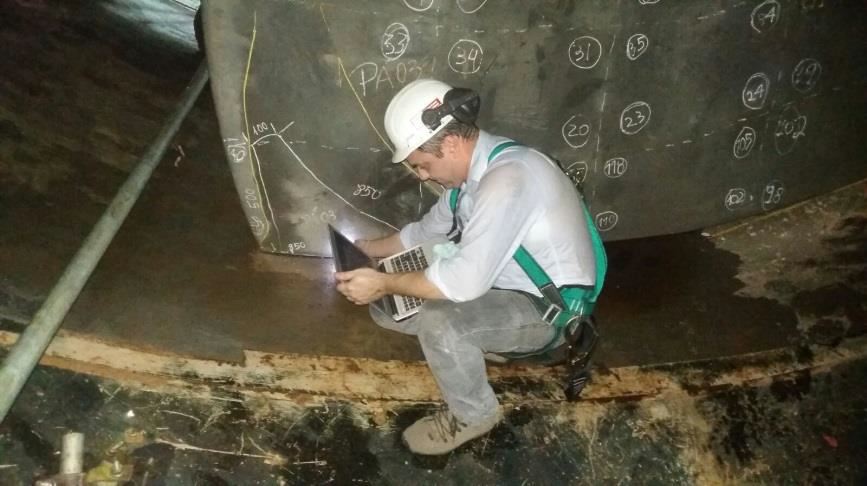
\includegraphics[width=0.9\linewidth, height=4cm]{figs/manolo} 
\caption{A equipe técnica analisa a pá verificando o desgaste do coating
existente e se existem danos a pá em si.}
\label{fig:subim1}
\end{figure}

\begin{figure}[H] 
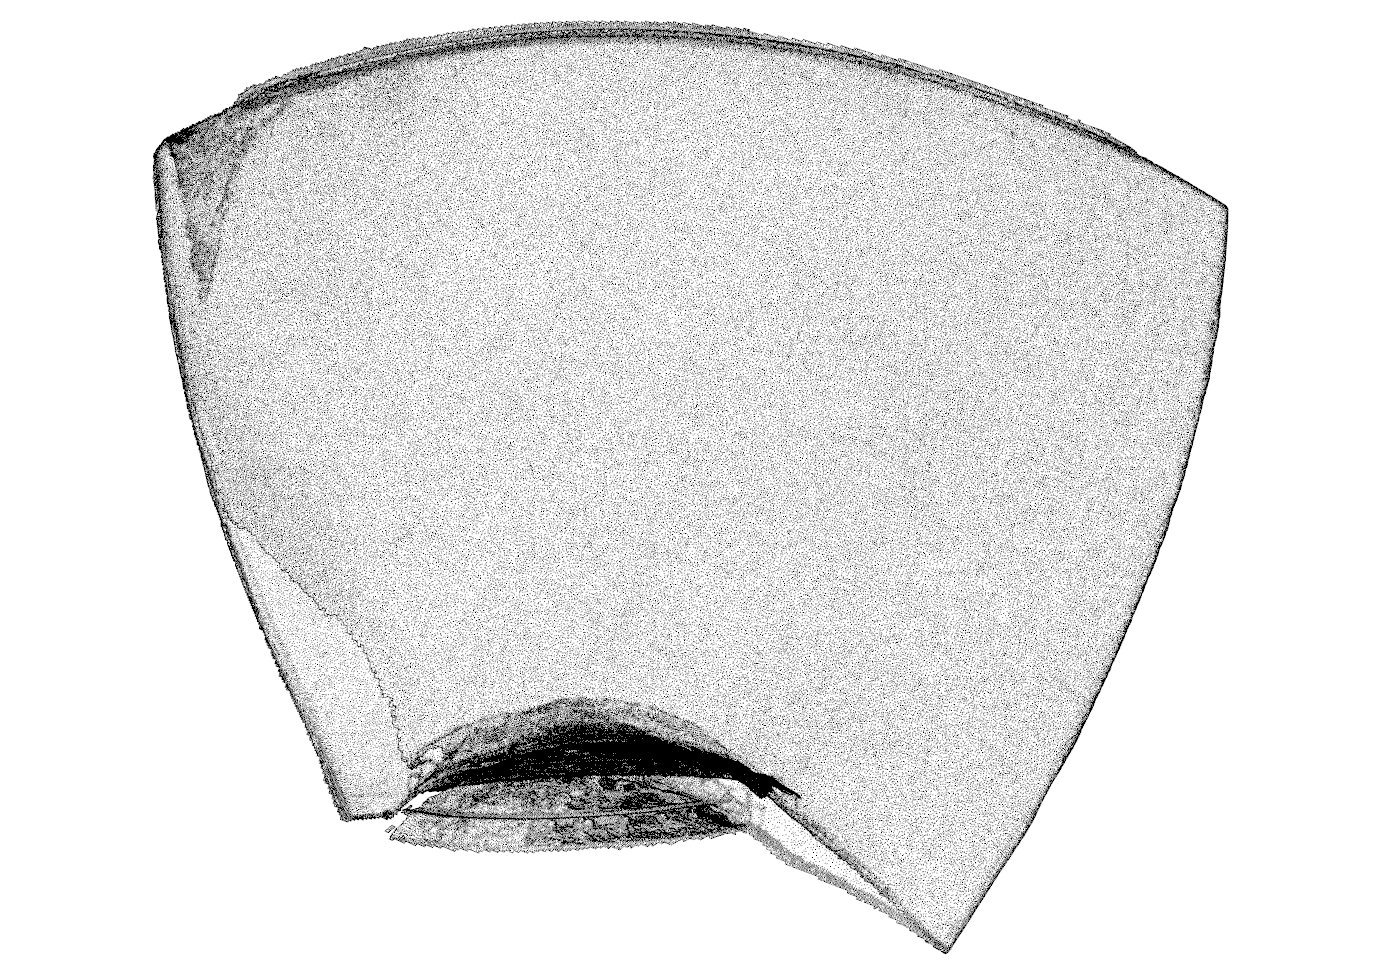
\includegraphics[width=0.9\linewidth, height=4cm]{figs/modelo_pa_faro}
\caption{Dado a necessidade de reparo um laser scanner de metrologia é
utilizado para mapear o dano com uma precisão de 2mm.}
\end{figure}

\begin{figure}[H]
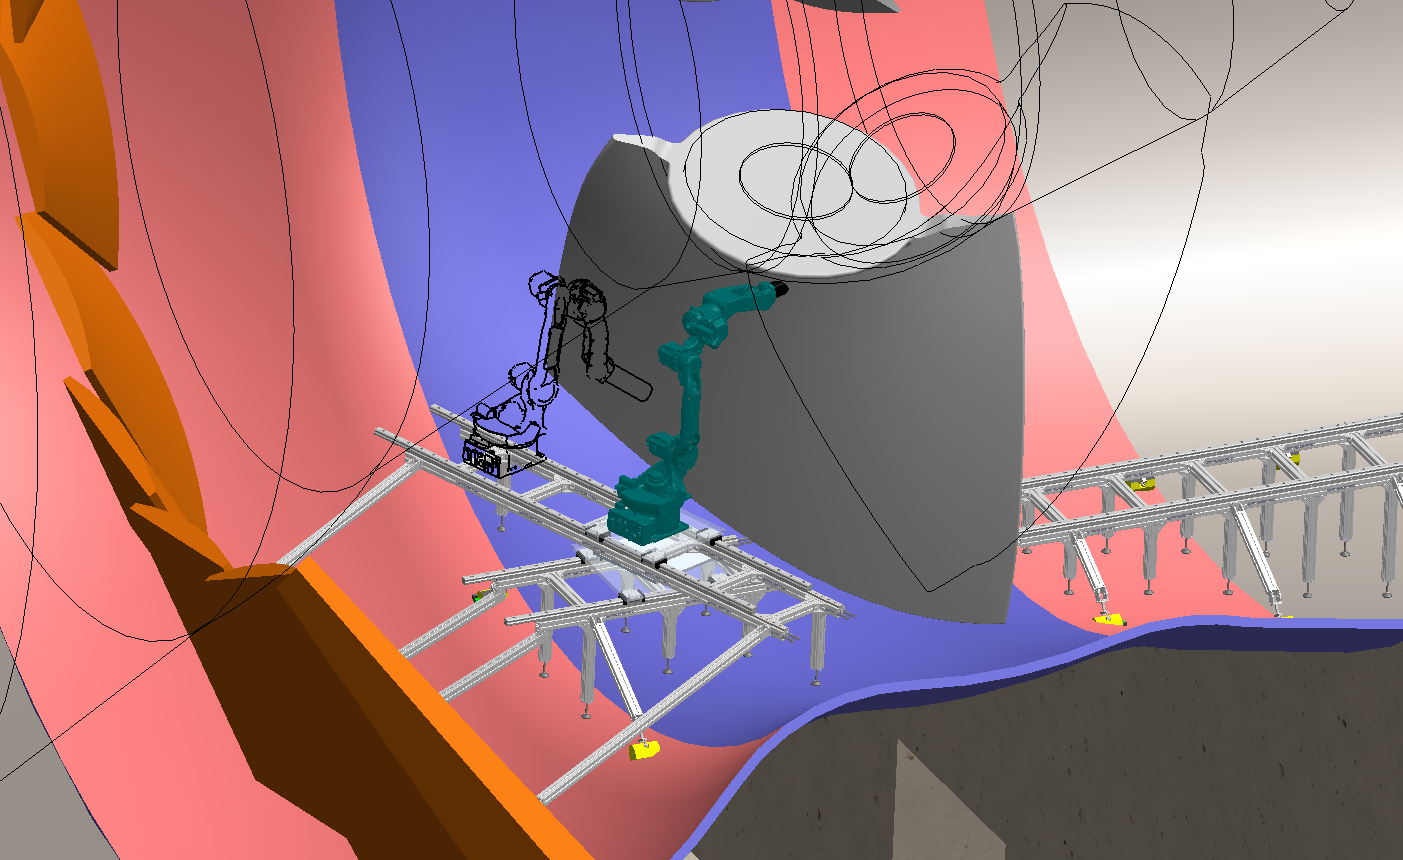
\includegraphics[width=0.9\linewidth, height=4cm]{figs/EMMA_Base_Secundaria_01} 
\caption{Um trilho modular é instalado no ambiente e aconrado através de pinos
magnéticos. O trilho é utilizado para levar o manipulador até a pá e movimentar
o manipulador ao longo da área de trabalho.}
\end{figure}

\begin{figure}[H]
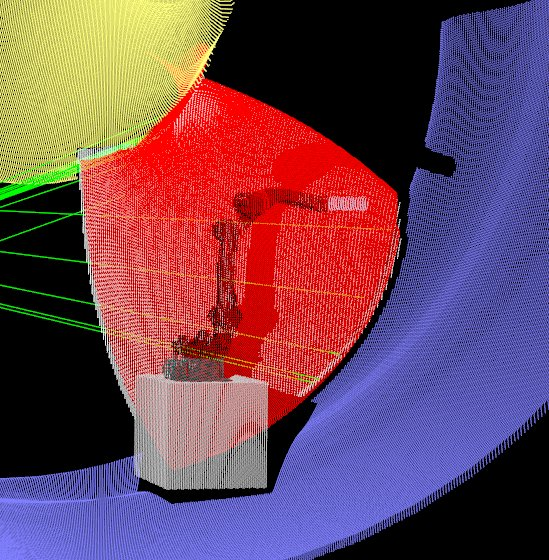
\includegraphics[width=0.9\linewidth, height=4cm]{figs/localizacao}
\caption{Algoritmo de processamento de nuvens de pontos analisam um scan laser
do ambiente e estimam a posição relativa entre o manipulador e a pá.}
\end{figure}


% \begin{figure}[H] 
% \begin{subfigure}{0.5\textwidth}
% 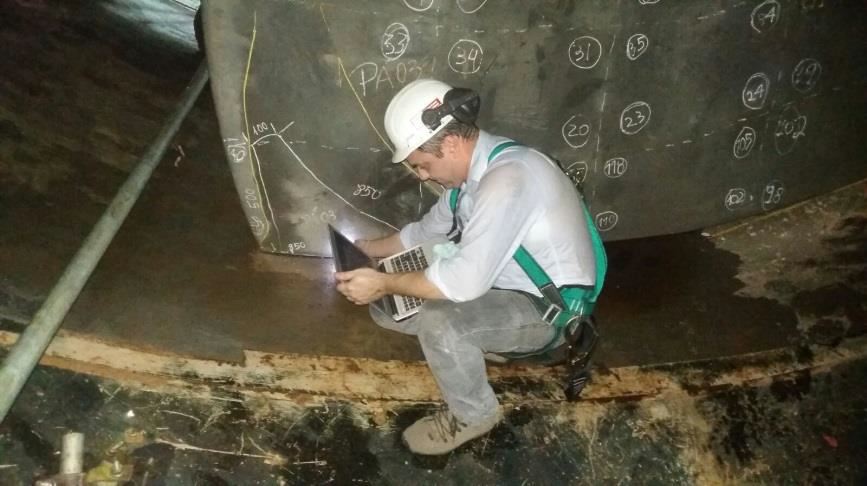
\includegraphics[width=0.9\linewidth, height=4cm]{figs/manolo} 
% \caption{A equipe técnica analisa a pá verificando o desgaste do coating
% existente e se existem danos a pá em si.}
% \label{fig:subim1}
% \end{subfigure}
% ~
% \begin{subfigure}{0.5\textwidth}
% \label{fig:subim2}
% 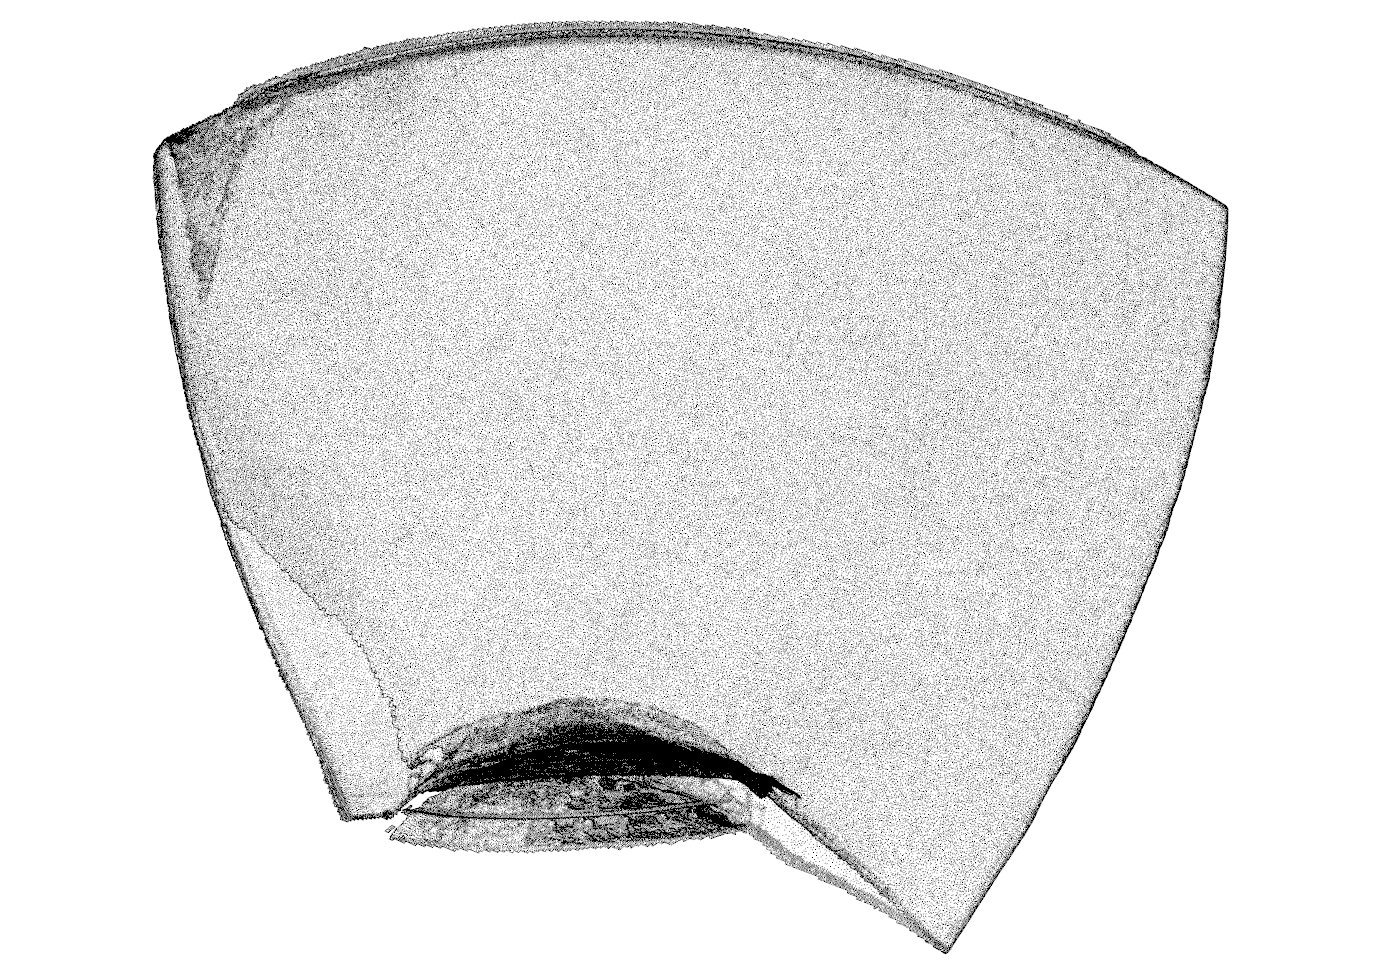
\includegraphics[width=0.9\linewidth, height=4cm]{figs/modelo_pa_faro}
% \caption{Dado a necessidade de reparo um laser scanner de metrologia é
% utilizado para mapear o dano com uma precisão de 2mm.}
% \end{subfigure}
%  \label{fig:image2}
% \end{figure}
% 
% \begin{figure}[H]
% \ContinuedFloat
% \begin{subfigure}{0.5\linewidth}
% 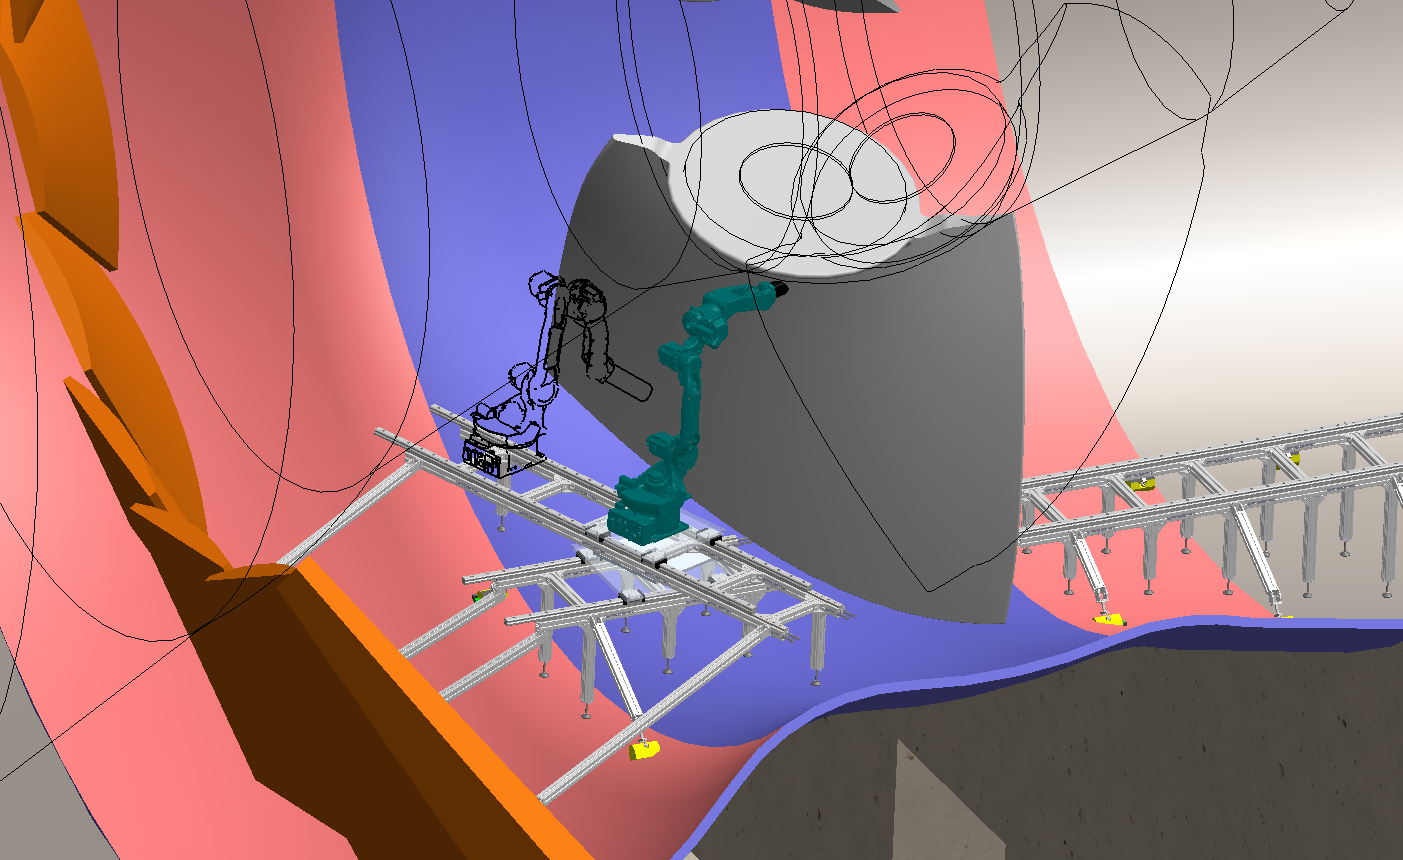
\includegraphics[width=0.9\linewidth, height=4cm]{figs/EMMA_Base_Secundaria_01} 
% \caption{Um trilho modular é instalado no ambiente e aconrado através de pinos
% magnéticos. O trilho é utilizado para levar o manipulador até a pá e movimentar
% o manipulador ao longo da área de trabalho.}
% \end{subfigure}
% ~
% \begin{subfigure}{0.5\linewidth}
% \label{fig:subim2}
% 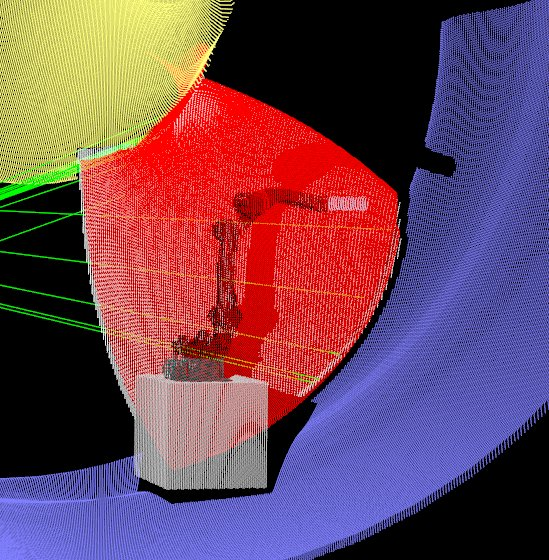
\includegraphics[width=0.9\linewidth, height=4cm]{figs/localizacao}
% \caption{Algoritmo de processamento de nuvens de pontos analisam um scan laser
% do ambiente e estimam a posição relativa entre o manipulador e a pá.}
% \end{subfigure}
%  \label{fig:image2}
% \end{figure}



% \begin{figure}[h!]
% \centering
% \captionsetup[subfigure]{position=b}
% \caption{3D printed wax mould post processing}
% \label{fig:Mould}
% \subcaptionbox{Um trilho modular é instalado no ambiente e aconrado através de pinos
% magnéticos. O trilho é utilizado para levar o manipulador até a pá e movimentar
% o manipulador ao longo da área de
% trabalho.\label{fig:MouldWithSupport}}{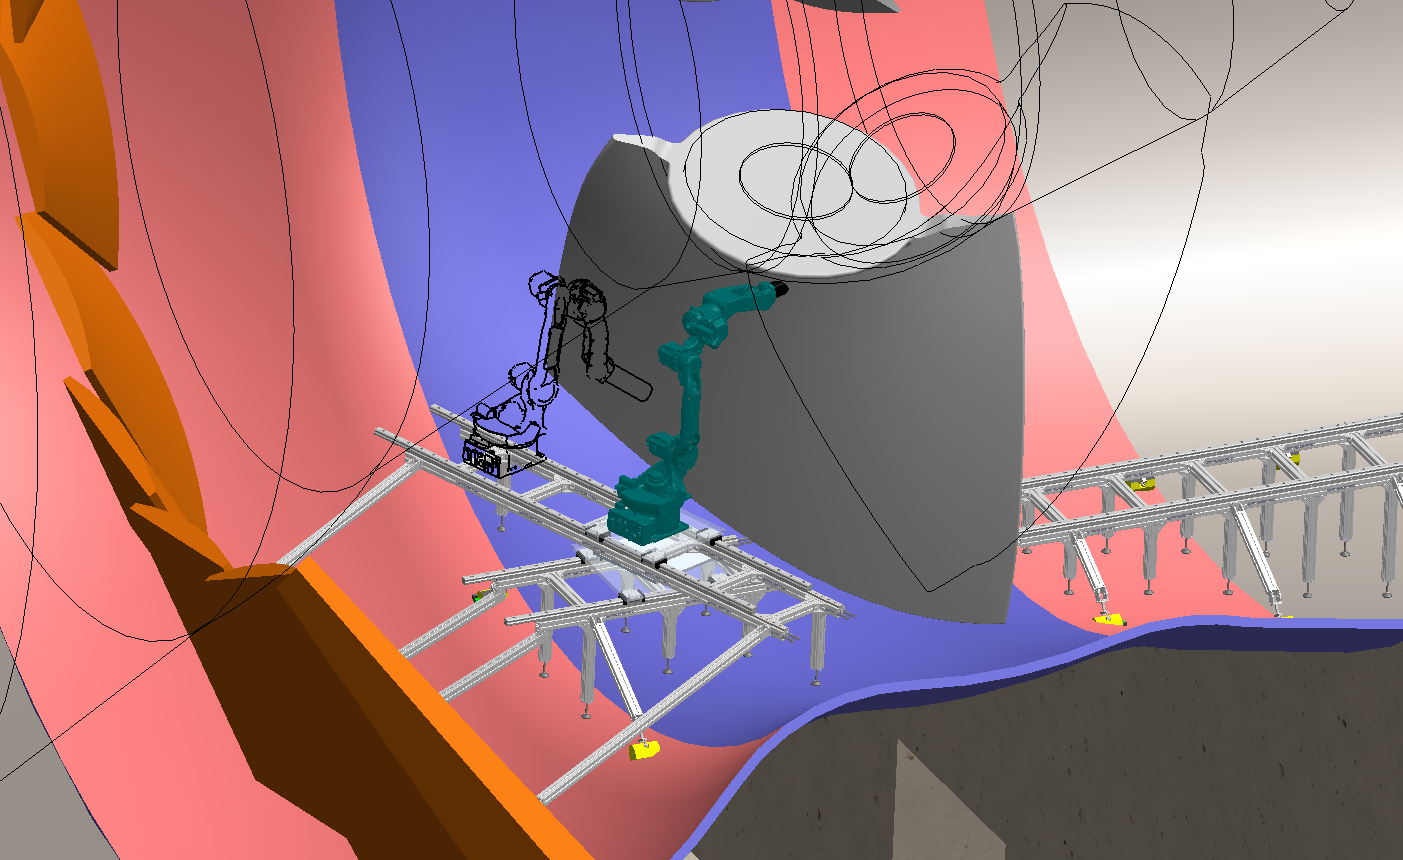
\includegraphics[width=0.5\linewidth, height=4cm]{figs/EMMA_Base_Secundaria_01}}
% \subcaptionbox{Algoritmo de processamento de nuvens de pontos analisam um scan laser
% do ambiente e estimam a posição relativa entre o manipulador e a pá.
% \label{fig:MouldAfterWashing}}{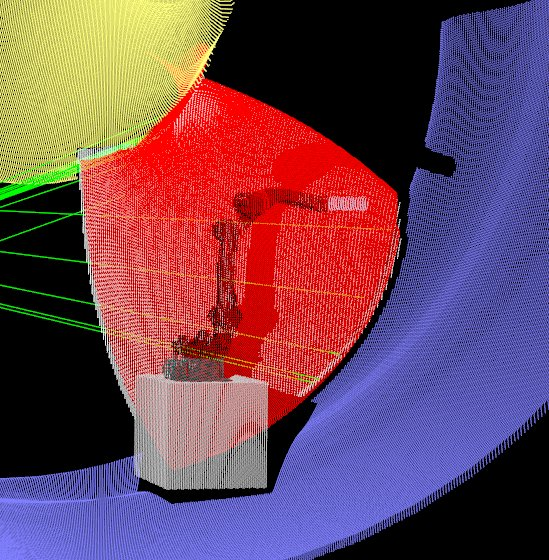
\includegraphics[width=0.5\linewidth, height=4cm]{figs/localizacao}}
% \end{figure}
% \end{document}









\begin{figure}[H]
\ContinuedFloat
\begin{subfigure}{0.5\textwidth}
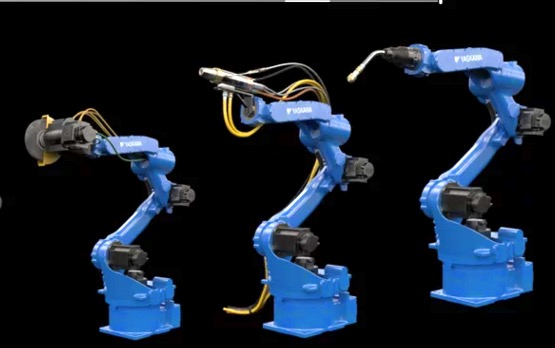
\includegraphics[width=0.9\linewidth, height=4cm]{figs/robots_evo} 
\caption{O equipamento necessário para a tarefa, seja soldagem, esmerilhamento
ou coating é instalado no manipulador e o ambiente e superfície são preparados.}
\end{subfigure}
~
\begin{subfigure}{0.5\textwidth}
\label{fig:subim2}
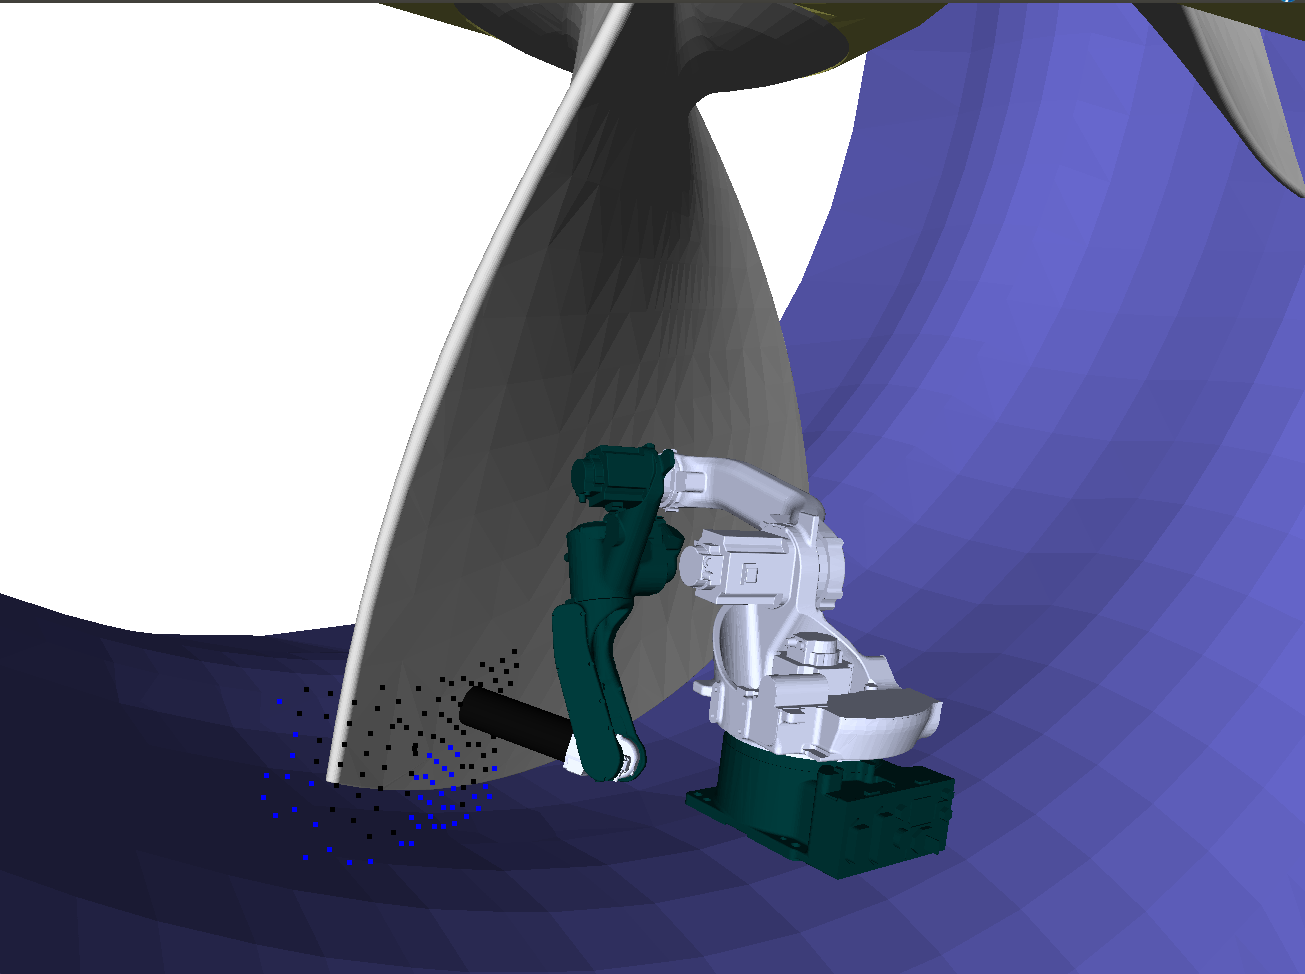
\includegraphics[width=0.9\linewidth, height=4cm]{figs/footleft}
\caption{O algoritmo estima e executa a trajetória para a tarefa planejada.}
\end{subfigure}
 \label{fig:image2}
\end{figure}

O resultado do processo é uma pá restaurada e protegida, aumentando a eficiência
de geração e vida útil da mesma. 

\section{Motivação}

Desgastes por corrosão, erosão e abrasão em pás de turbinas de hidroelétricas
resultam em perda do perfil hidráulico, reduzindo assim a eficiência de geração.
O desgaste reduz também a vida útil da turbina, o tempo de operação entre
paradas de manutenção, assim como, aumentam os custos de manutenção e o tempo
necessário de parada de máquina para a realização do reparo. Logo, significa uma
perda da eficiência de geração, e por consequente um impacto econômico
significativo na operação.
A aplicação de revestimento aumenta a resistência do material contra os
desgastes, custando em torno de 20\% do valor de uma peca nova e representando
um aumento da vida útil em mais de 300\%. Entretanto, dados as limitações da
tecnologia atual, só é possível aplicar o revestimento em bancada, logo, antes
da instalação das pás. Logo, o desenvolvimento tecnológico que possibilite
reaplicar a camada de revestimento dentro do circuito hidráulico resultaria em
um ganho significativo na geração e redução dos custos de operação.
Antes de aplicar o revestimento é necessário reparar a pá recuperando o perfil
hidráulico da mesma, quanto maior a precisão da recuperação do perfil hidráulico
maior a eficiência de geração. Logo, a robótica se torna a ferramenta ideal para a tarefa.

\section{Objetivo}

O objetivo geral do projeto é desenvolver e testar uma metodologia que permita
utilizar a robótica para reparar e revestir pás instaladas em circuitos hidráulicos.

Os objetivos específicos são determinar as metodologias: 

\begin{itemize}
  \item definir o manipulador ótimo para cada hidroelétrica 
  \item movimentar o manipulador dentro do circuito hidráulico
  \item estimar a posição do manipulador com relação ao meio
  \item material e técnica de coating e reparo 
  \item preparar o meio e superfície
  \item logística para instalar um sistema robótico no circuito hidráulico
  \item determinar os riscos associados
  \item planejar e executar a manipulação
  \item representar as diferentes informações do processo para um operador
  \item verificar as perdas de carga do processo de revestimento
  \item integrar e utilizar as diversas ferramentas
  \item mapear o perfil hidráulico e medir os danos
\end{itemize}

\section{Originalidade}

Não existe nenhuma solução ou estudo realizado sobre a aplicação de revestimento
dentro do circuito hidráulico sem desinstalar as pás da turbina. A aplicação de
revestimento para proteção contra abrasão, cavitação, corrosão e erosão em peças
de turbinas de hidrelétricas realizado atualmente é limitada a trabalho em
bancada com a peça desinstalada. O desafio de realizar o trabalho de
revestimento dentro do circuito hidráulico se dá pela dimensão da escotilha de
acesso, que limita o tamanho do robô, pelo posicionamento do robô com relação a
pá da turbina, que se encontra a alguns metros do solo, pelo processo de
aplicação que requer velocidade constante utilizando uma pistola pesada e pelo
controle de temperatura e humidade necessários. Esta pesquisa é inovadora no
setor elétrico brasileiro e é um avanço com relação ao estado da arte.

\section{Aplicabilidade}

A metodologia desenvolvida no projeto  poderá ser aplicada na maioria das
hidroelétricas de médio ou grande porte. A metodologia determina o tamanho e
modelo de manipulador ótimo para o circuito hidráulico em questão, assim como,
qual material de coating a ser aplicado. A restrição para aplicação da tecnologia é
apenas dada pelo espaço entre as pás, em hidroelétricas de pequeno porte a arma
de coating não cabe entre as pás. Logo, a abrangência é nacional, entretanto com
restrição de uso em pequenas unidades geradoras.

\section{Relevância}

A matriz geradora Brasileira é constituída em sua maioria por geração
hidráulica, com um grande número de centrais em rios tipos corredeiras que
possuem reservatórios pequenos. Neste tipo de rio não há tempo de sedimentação
das partículas sólidas na água, essas partículas sólidas, mesmo em quantidades
pequenas, geram um elevado nível de desgaste por erosão e cavitação. Logo, o
projeto é de relevância para o setor elétrico e para a nação, pois aumenta a
eficiência da matriz energética Brasileira, aumenta a disponibilidade da máquina
para geração e reduz os custos de manutenção, representando uma melhora
econômica e social.

\section{Capacitação}

A pesquisa e o desenvolvimento (P\&D) tem como propósito fomentar o avanço
tecnológico e novas maneiras de desenvolver um tipos específicos de conhecimento
no país. O desenvolvimento do EMMA, no âmbito P\&D é um exemplo de como a
parceria entre agências do governo, empresa e universidades podem colaborar para
a capacitação tecnológica e o desenvolvimento de novas tecnologias.

O projeto EMMA possui 4 pesquisadores inscritos no mestrado. Os temas são todos
a pesquisa no campo da robótica, sendo a previsão de conclusão das teses
esperada para a fase 2 e fase 3 do EMMA. Os alunos de mestrado e seus
respectivos cursos são:

\begin{itemize}
  \item Estevão Fróes Ferrão, Programa de Engenharia Mecânica/COPPE, Rio de
  Janeiro
  \item Gabriel Alcantara Costa Silva, Programa de Engenharia Elétrica/COPPE,
  Rio de Janeiro
  \item Eduardo Elael de Melo Soares, Programa de Engenharia Elétrica/COPPE, Rio
  de Janeiro
  \item Julia Ramos Campana, Departamento de Artes e Design, PUC, Rio de Janeiro
\end{itemize}

Para o comprimento dos requisitos de segurança do Ministério do Trabalho e
Emprego, a equipe do projeto foi submetida à capacitação em segurança, nas
normas relevantes às situações encontradas no interior do circuito hidráulico. As certificações foram nas
seguintes normas:

\begin{itemize}
  \item NR10 - Segurança e Instalações e Serviços em Eletricidade
  \item NR33 - Segurança e Saúde nos Trabalhos em Espaços Confinados
  \item NR35 - Trabalho em Altura
\end{itemize}

Os seguintes pesquisadores foram capacitados no curso:

\begin{itemize}
  \item Estevão Fróes Ferrão, Programa de Engenharia Mecânica/COPPE
  \item Gabriel Alcantara Costa Silva, Programa de Engenharia Elétrica/COPPE
  \item Renan Sales de Freitas, Programa de Engenharia Elétrica/COPPE
  \item Eduardo Elael de Melo Soares, Programa de Engenharia Elétrica/COPPE
  \item Julia Ramos Campana %TODO Julia departamento
\end{itemize}
A pesquisa no projeto EMMA proporcionou a elaboração de dois artigos
submetidos/publicados em revistas, abordando os seguintes tópicos: 

\begin{itemize}
  \item Estado da arte e design conceitual de soluções robóticas para
  revestimento de turbinas hidráulicas \textit{in situ} (State of the art and
  conceptual design of robotic solutions for \textit{in situ} hard coating of
  hydraulic turbines).
  \item Solução Conceitual e estudo de viabilidade técnica para para
  revestimento de turbinas hidráulicas \textit{in situ} (EMMA - A robotic
  system for \textit{in situ} hydropower turbine hard coating).
\end{itemize}

\section{Razoabilidade dos Custos}

Atualmente, após a instalação da unidade geradora, não existe método disponível
para proteger a ogiva geradora contra os desgastes de sua utilização. Sendo,
infelizmente, a recuperação sempre o caminho e isso pode ser estimado entre 90 e
120 dias de UG parada. A frequência de paradas de recuperação variam dependendo
da idade da unidade geradora, material, tipo de bacia e etc. A única certeza é
que um dia será necessário. A aplicação de revestimento pode ser realizada
durante as paradas planejadas, sem perda de tempo de geração.
De acordo com a tabela de situação de cavitação em turbina hidráulica no Brasil
(Out/97), em média 5 unidades geradoras apresentaram  cavitação a cada 24.071
horas de operação (2,7 anos), das 36 instalações analisadas. Logo, em Jirau a
aplicação do revestimento in situ significaria em um aumento da disponibilidade
de geração de 600 dias a cada 2,7 anos, considerando turbinas de 75 MW de
potencia, seria equivalente a 1.080.000 MW a cada 2,7 anos.

\section{Metodologia adotada}

O projeto EMMA foi dividido em 3 fases, sendo cada fase um projeto distinto.
Cada fase avançando a tecnologia ao longo da cadeia de inovação. Na primeira
fase foi desenvolvido a metodologia/conceito. Na segunda fase será feito o
desenvolvimento experimental testando o sistema de coating. Na terceira fase
será expando a solução para incluir reparo e validar a tecnologia em outras
centrais hidroelétricas.

Ao início da primeira fase não se sabia se existiria uma solução para o
problema. Os requisitos de acesso, operação e coating são extremamente
limitantes. A metodologia adotada na fase 1 para desenvolver o conceito da
solução foi:

\textbf{Etapa 1}: Levantamento dos requisitos do ambiente, tarefas e
procedimentos.
Estudo do estado da arte e bibliografias existente no tópico. Baseado nos
requisito e estado da arte foi definido uma solução conceito que atende ao problema.

\textbf{Etapa 2}: A solução conceito foi detalhada. Neste detalhamento foi
determinando os equipamentos e fornecedores que seriam adequados a serem
utilizados na solução. Assim como foi realizado pesquisa bibliográfica para
determinar quais os algoritmos e técnicas mais adequadas a serem implementadas
como parte da solução.

\textbf{Etapa 3}:  A solução conceito detalhada foi validada através de
simulações e experimentos em laboratório de alguns conceitos chaves. Um exemplo
foi utilizar o openrave para simular o processo de movimento do manipulador e
experimentos de campos da fixação por pino magnético.

\section{Estratégia de difusão}

A estratégia de difusão adotada no projeto foi a realização de um evento de
transferência de conhecimento dentro da faculdade de porto velho que inclui não
apenas os funcionários da ESBR, mas também os alunos e professores da faculdade.
O evento serviu como um “aulão” em pesquisa aplicada em robótica. Onde cada
pesquisador do projeto, em sua maioria alunos de mestrado da UFRJ, deram uma
aula sobre seus tópicos de pesquisa dentro do projeto.

%TODO foto do evento

\section{Melhorias de processo, equipamento e sistema}

O projeto representa uma melhoria no processo de reparo das pás de turbina
hidroelétricas que atualmente são feitas manualmente. Espera-se que o processo
robótico consiga recuperar o perfil hidráulico para uma margem de 2-5 mm do perfil original.

O fato de o EMMA também realizar o revestimento das turbinas instaladas, algo
antes impossível, o projeto representa uma melhoria no equipamento (pás das
turbinas), pois as mesmas se tornam mais resistentes aos danos corrosão, erosão e abrasão.

Por fim, o projeto também representa uma melhoria a todo sistema de geração de
energia elétrica. Pois, aumenta a vida útil das turbina e mantêm o perfil
hidráulico original, logo um impacto direto no aumento da geração.

\section{Pesquisa Correlatas}

\textbf{Google Schoolar, IEEE, Field Robotics, ... }: nenhum resultado foi
encontrado na revisão bibliográfica para uma solução robótica de aplicação de
revestimento em turbinas hidroelétrica já instaladas no Brasil e no exterior. A
pesquisa revela apenas o desenvolvimento de robôs para reparos in situ da
turbina, capazes de realizar soldagem, em exemplo RoboTurb da UFSC e Scompi da
Hydro-Quebec. Ambos não aplicáveis ao problema de revestimento devido as
limitações do manipulador robótico nos sistemas.

\textbf{INPI}: Nenhuma patente foi encontrada que se enquadre como o produto
objeto da pesquisa e desenvolvimento aqui proposta.

\textbf{ANEEL}: nenhum resultado foi encontrado na base de dados da ANEEL
relevante a um robô para revestimento. Os resultados encontrados referiam-se a
um Robo que inspeciona e corrige problemas em linhas de transmissão; Sistema
Multi-robôs Aéreos para Inspeção de Linhas e Robô para Inspeção Visualde
caldeiras.

\section{Instituição e Equipe}

O LEAD (Laboratório de Controle e Automação, Engenharia de Aplicação e
Desenvolvimento) é fruto de uma parceria entre a Petrobras e a Universidade
Federal do Rio de Janeiro (UFRJ) que visa ao desenvolvimento de novas
tecnologias na área de Automação e Controle.
Na avaliação da estatal brasileira de petróleo, ‘‘o laboratório reforça a
estratégia de desenvolvimento em conjunto de novas tecnologias, o que traz
benefícios tanto para as universidades, que realizam suas pesquisas acadêmicas
em laboratórios de ponta, quanto para a Petrobras que, ao compartilhar
conhecimentos, cria competências para superar seus desafios tecnológicos e
empresariais”.

DARLAN PARAGRAFO RIJEZA

%TODO DARLAN PARAGRAFO RIJEZA

A equipe técnica alocada para a realização do projeto EMMA:

\begin{itemize}
  \item Renan Salles de Freitas, Engenheiro de Controle e
Automação pela UFRJ, Rio de Janeiro, Brasil, e Candidato a Mestre em Ciências em Engenharia Elétrica
pelo Programa de Engenharia Elétrica, COPPE/UFRJ, Rio de Janeiro, Brasil. No
projeto EMMA, Renan é membro da equipe de Controle e Robótica, e responsável
pelas seguintes atividades: Manipuladores industriais: pesquisa de
mercado, análise cinemática, dinâmica e controle; Desenvolvimento do ambiente de
simulação para análise de soluções; Análise de viabilidade técnica do EMMA pela
visão da robótica e do controle; Desenvolvimento e simulação de algoritmos de
planejamento de trajetória.

  \item Estevão Fróes Ferrão possui graduação em Engenharia Mecânica pela Universidade
Federal do Rio de Janeiro (UFRJ), atualmente cursando o mestrado no Programa de Engenharia
Mecânica (PEM-COPPE/UFRJ). Faz parte da equipe do Projeto EMMA, como
Pesquisador/Engenheiro contratado pelo LEAD. Atua na área de Projeto Mecânico,
sendo resposável pela pesquisa, projeto e desenvolvimento de uma solução
mecânica para uma base com graus de liberdade que permitem o posicionamento do
robô utilizado.

\item Julia Ramos Campana é formada em Comunição Técnica e Mídia pelo Instituto de
Tecnologia e Illinois, pós graduada em Design Digital pela Vancouver Film School
e em Gerenciamento de Projeto pela Universidade da Columbia Britânica, é
atualmente aluna do Mestrado em Design pela PUC-RJ. Julia exerce a função de
Designer de interface e Usabilidade no projeto EMMA, trabalhando no
desenvolvimento do software de controle do sistema EMMA e em todas as questões
relacionadas aos usuários, testes e interações humano-automação da pesquisa.
\item Eduardo Elael de Melo Soares, Engenheiro de Controle e Automação pela UFRJ, Rio
de Janeiro, Brasil, e mestrando em Ciências em Engenharia Elétrica pelo
Programa de Engenharia Elétrica, COPPE/UFRJ, Rio de Janeiro, Brasil. No projeto
EMMA, Eduardo é membro da equipe de Controle e Robótica, e responsável pelas
seguintes atividades: Manipuladores de pequeno porte: Pesquisa e análise
geométrica; Realimentação de segurança: Pesquisa de laser 1D para uso em tempo
real; Reconhecimento de ambiente: Escolha e adaptação de técnicas para
reconhecimento da posição do Robô no ambiente; Desenvolvimento e simulação de
algoritmos de planejamento de trajetória.
\item Gabriel Alcantara Costa Silva, Engenheiro de Controle e Automação pela
UFRJ, Rio de Janeiro, Brasil, e mestrando em Ciências em Engenharia Elétrica pelo
Programa de Engenharia Elétrica, COPPE/UFRJ, Rio de Janeiro, Brasil. No projeto
EMMA, Eduardo é membro da equipe de desenvolvimento de software para sistemas
robóticos, e responsável pelas seguintes atividades: Desenvolvimento de técnicas
em visualização, localização e mapeamento 3D; Identificação e
Localização de objetos; Integração do sistema.

\end{itemize}








    
    
  


\chapter{Plano de Projeto}\label{chap::planejamento}


\section{Etapa 1 - Fundação Coppetec}

\begin{figure}[H]
\centering
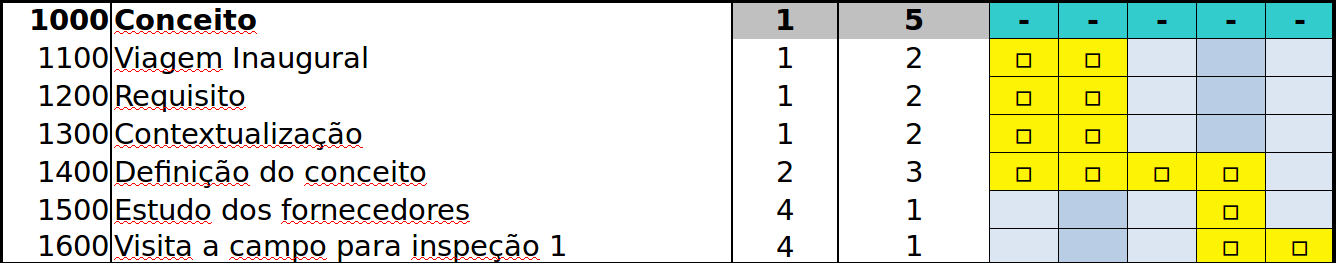
\includegraphics[width=0.9\columnwidth]{figs/etapa1_completo}
\end{figure} 

\textbf{1000 Conceito:} A etapa 1000 do projeto foi executada como prevista. O
objetivo da etapa foi a determinação dos requisitos do problema e concepção de
possíveis soluções. As seguintes trabalhos foram executados dentro desta etapa

\noindent
\textbf{1100 Viagem Inaugural:} Assinatura do termo inaugural do projeto e
análise em campo da problemática

Etapa executada como previsto. 

\begin{figure}[H]
\centering
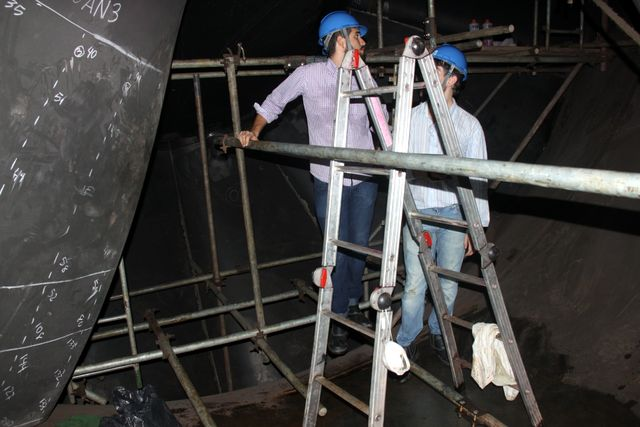
\includegraphics[width=0.6\columnwidth]{figs/img_4967}
\caption{Pesquisadores analisando o ambiente.}
\end{figure}

\noindent
\textbf{1200 Requisito:} Fazer levantamento dos requisitos que afetam a
instalação e utilização de um robô dentro circuito hidráulico.

Etapa executada como previsto. Foram levantados todos os requisitos de acesso,
ambiente e processo de coating.

\noindent
\textbf{1300 Contextualização:} Levantamento das tecnologias existentes no para
aplicações de revestimento em ambientes confinados.

Etapa executada como previsto. Diversas tecnologias foram pesquisadas, como o
robô scompi da hidroquebec. Nenhuma das soluções atuais atendiam os requisitos
de operação do projeto.

\noindent
\textbf{1400 Definição dos conceitos:} Definição de uma solução de um robô capaz
de operar no ambiente e realizar tarefas de revestimento.

Etapa executada como previsto. Foram levantados 3 conceitos viáveis, os quais
foram analisados chegando ao conceito proposto dentro do projeto. Utilizar um
manipulador industrial, acessando o circuito hidráulico pela escotilha de
acesso, com movimentação através de trilhos modulares e alinhamento, mapeamento
e planejamento de trajetória baseado em scan 3D a laser do ambiente.

\begin{figure}
\centering
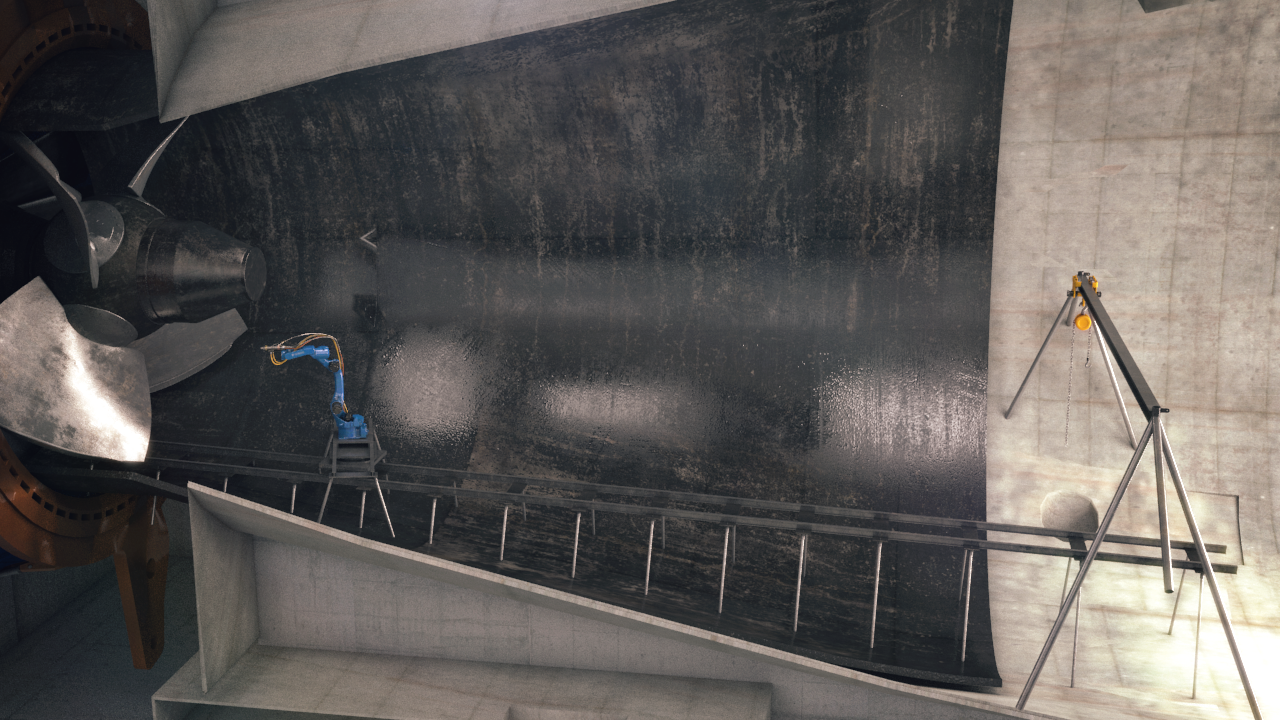
\includegraphics[width=0.9\columnwidth]{figs/turbine_evo}
\caption{Solução conceito.}
\end{figure}

\noindent
\textbf{1500 Estudo dos fornecedores:} Definição dos fornecedores do equipamento
necessário para a pesquisa

Etapa executada como previsto. Foram analisados mais de 50 modelos de
manipuladores distintos, sendo que 5 atendiam os requisitos do problema como
possíveis soluções.

\begin{figure}[h!]
\centering
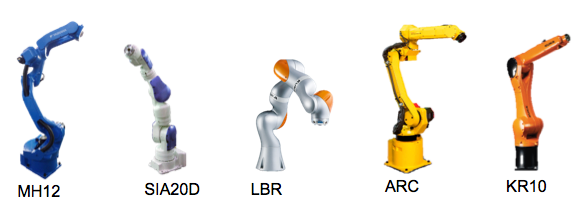
\includegraphics[width=0.9\columnwidth]{figs/robots}
\caption{Possíveis modelos de manipuladores que atendem os requisitos.}
\end{figure}

\noindent
\textbf{1600 Visita a campo para inspeção 1:} foi realizada uma visita inicial
a campo para juntamente com revisão bibliográfica sobre o tema “desgaste”
coletar dados de campo através de inspeção nas pás das turbinas. Essas inspeções
foram realizadas ao longo do projeto para confrontar com o que existe na
bibliografia.


\section{Etapa 02}

\begin{figure}[H]
\centering
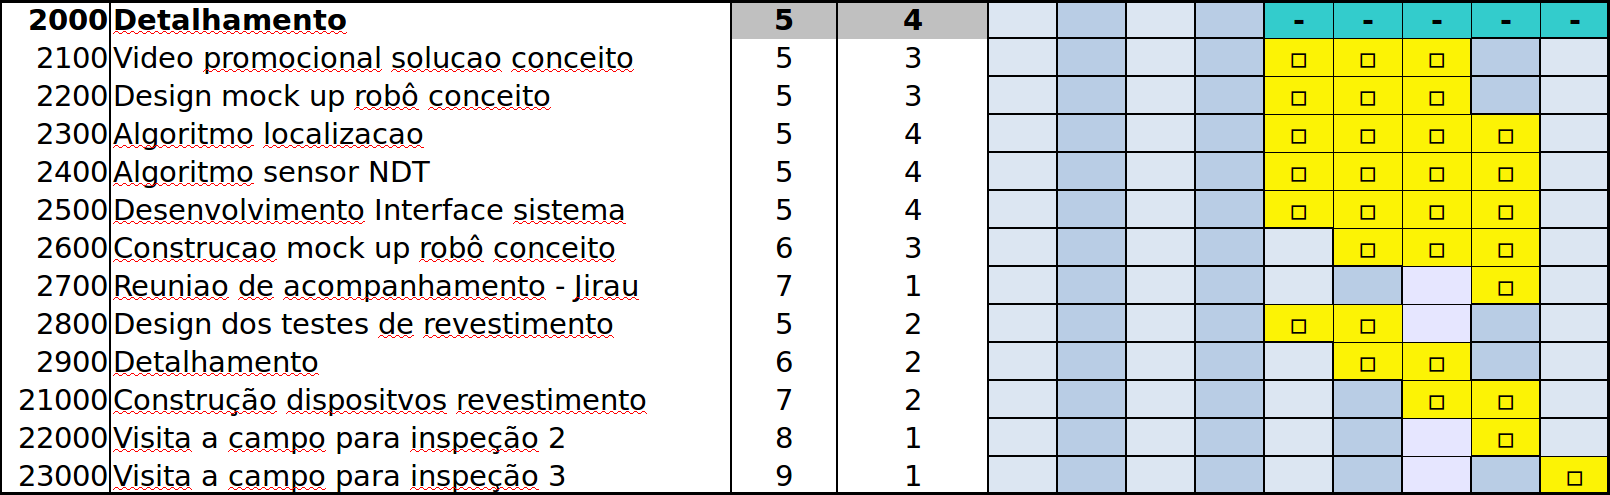
\includegraphics[width=0.9\columnwidth]{figs/etapa2_completo}
\end{figure} 

\noindent
\textbf{2000 Detalhamento:} A etapa 2000 do projeto foi executada existindo
variações entre previsto e executado. O objetivo da etapa foi a análise das
proposições mediante estudos teóricos e design detalhado da possível solução e sistema

\noindent
\textbf{2100 Video promocional solução conceito:} Animação 3D da solução
conceito

Houve atraso no processo de contratação e aprovação do script. A tarefa foi
executada com 3 meses de atraso. Entretanto, o mesmo não impactou no projeto,
pois não era uma tarefa de pré-requisito.

\noindent
\textbf{2200 Design mock up robô conceito:} Design em CAD / Solidworks do
conceito do robô

Tarefa executada como prevista. Foram realizado diversos designs para possíveis
bases para a solução conceito, assim como análises geométricas, cinemática,
dinâmica e de manipulabilidade para definir o manipulador.

\begin{figure}\centering
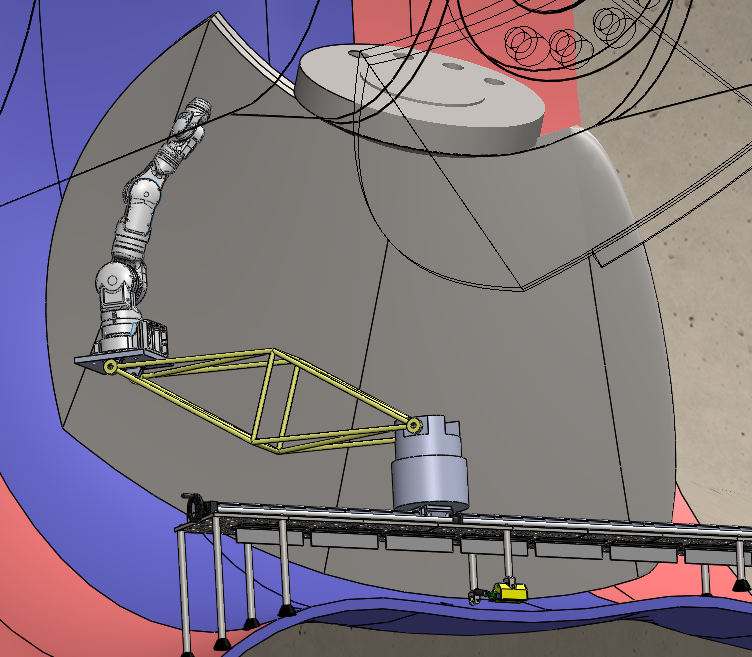
\includegraphics[width=0.6\columnwidth]{figs/EMMA_Base_Conceito_PRR}
\caption{Possível base para o manipulador dentro do ambiente do circuito
hidráulico.}
\end{figure} 


\noindent
\textbf{2300 Design dos testes de revestimento:} %TODO DARLAN

\noindent
\textbf{2400 Algoritmo de localização:} definir o algoritmo/técnica que irá
localizar o robô com relação a turbina.

Tarefa executada como prevista. Foi determinado que o melhor e mais preciso
método é escanear o robô e a pá com um laser de metrologia e a estimar posição
relativa das nuvens de pontos resultantes.

\begin{figure}[H]
\centering
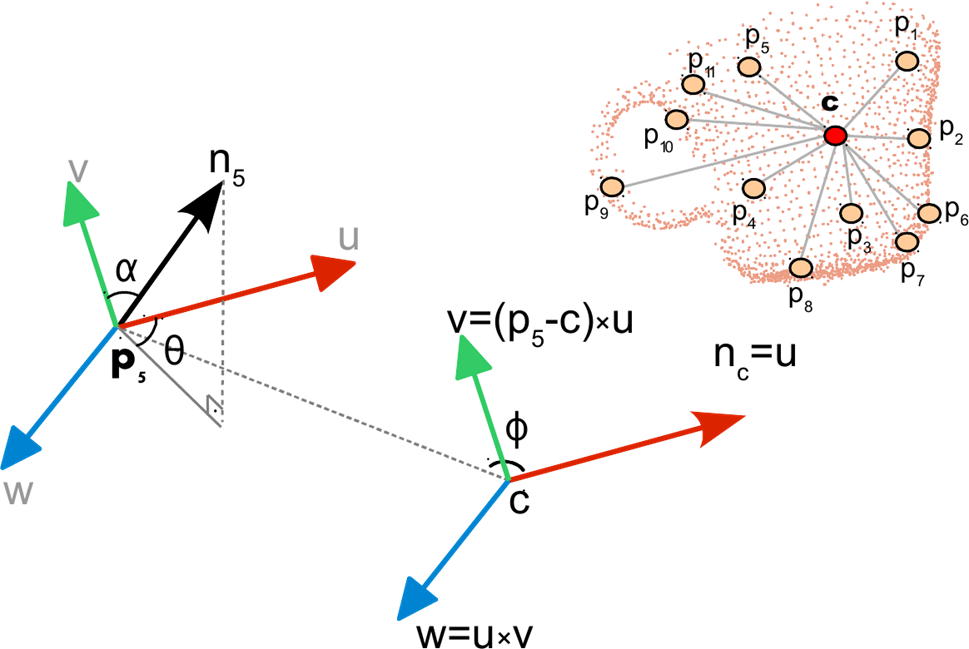
\includegraphics[width=0.6\columnwidth]{figs/pc_position}
\caption{Posição relativa entre duas nuvens de pontos.}
\end{figure} 

\noindent
\textbf{2500 Algoritmo sensor NDT:} Algoritmo que irá avaliar e mapear a
qualidade do revestimento.

Tarefa executada como prevista. Foi determinado que o método mais eficiente é
utilizar um humano para rapidamente realizar uma amostragem de alguns pontos com
sensor ultra-som manual. A solução robótica seria em uma alusão “matar um mosquito com basuca”.

\noindent
\textbf{2600 Desenvolvimento Interface sistema:} Interface gráfica de controle e
utilização do sistema

Essa tarefa foi estendida para 8 meses, se tornando uma teses de mestrado dada
sua complexidade. A solução conceito possui um volume muito grande de interação
e informação para o usuário. Logo, adotou-se um estudo metódico,
estabelecendo-se toda a metodologia para determinar a interface e como cada
informação será representada.

\noindent
\textbf{2700 Construção mock up robô conceito:} Construção do mock up do robô
que aplica o revestimento

Tarefa executada como previsto. Foi construído todo o ambiente do circuito
hidráulico e manipulador através de impressão 3D em uma escala 1:20.

\begin{figure}[h!]
\centering
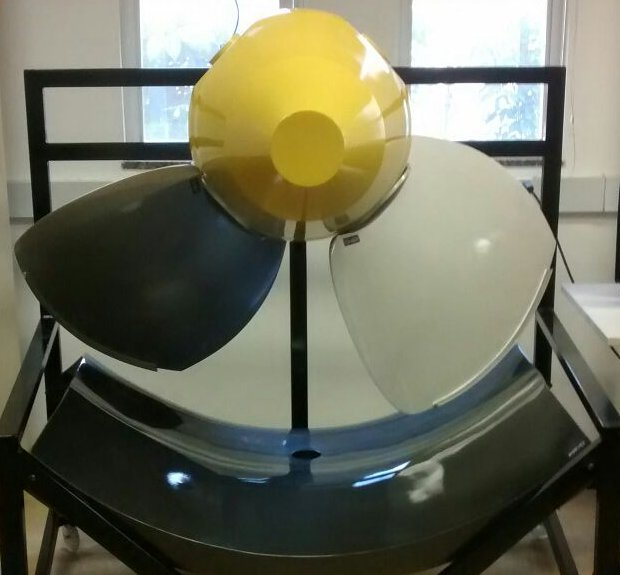
\includegraphics[width=0.6\columnwidth]{figs/maquete}
\caption{Maquete utilizada no desenvolvimento do conceito.}
\end{figure} 

  
\noindent
\textbf{2800 Design dos testes de revestimento:} %TODO DARLAN

\noindent
\textbf{2900 Reunião de acompanhamento:} Reunião de acompanhemento do projeto.
Tarefa executada como prevista.

\noindent
\textbf{21000 Construção dispositivos revestimento:}


\noindent
\textbf{22000 Visita a campo para inspeção 2:}


\noindent
\textbf{23000 Visita a campo para inspeção 3:}

\begin{figure}\centering
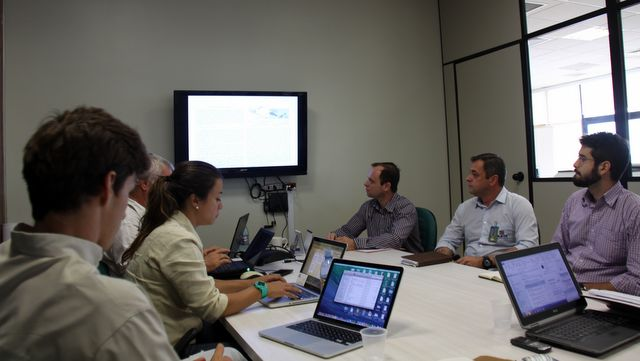
\includegraphics[width=0.6\columnwidth]{figs/img_4836}
\caption{Reunião de acompanhamento em Jirau.}
\end{figure} 

\section{Etapa 03} 

\begin{figure}[H]
\centering
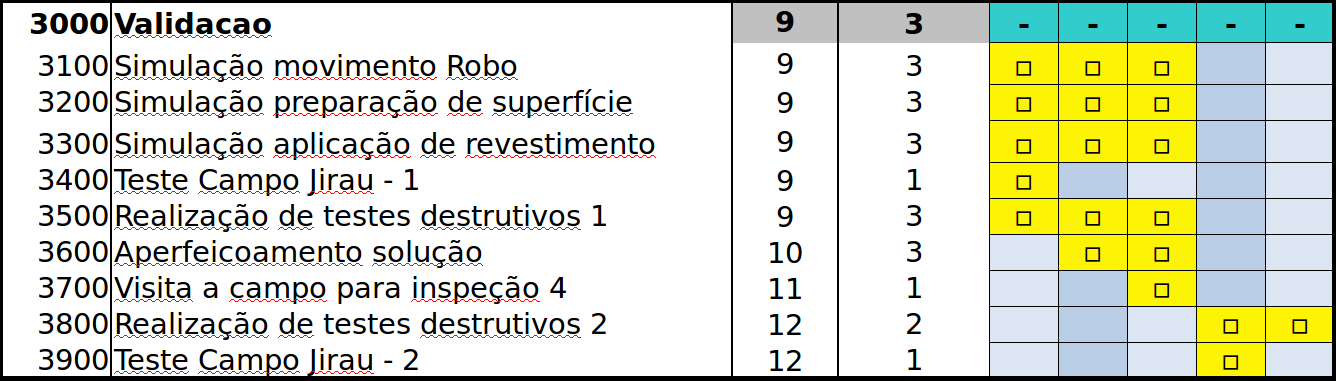
\includegraphics[width=0.9\columnwidth]{figs/etapa3_completo}
\end{figure} 

\noindent
\textbf{3000 Detalhamento:} A etapa 3000 do projeto foi executada existindo
variações entre previsto e executado. O objetivo da etapa é validação da solução
detalhada através de simulação e experimentos.

\noindent
\textbf{3100 Simulação movimento robô:} 
Simulação dos movimentos do robô sobre a turbina, verificando limites e singularidades

Tarefa executada como prevista. Foi utilizado o simulador Openrave.  

\noindent
\textbf{3200 Simulação preparação de superfície:}
Testes para avaliar a modificação do procedimento de jateamento para a sua adequação ao ambiente proposto no projeto;

\noindent
\textbf{3300 Simulação aplicação revestimento:}

Aplicação em amostras de testes para qualificação de materiais e procedimento de aspersão para posterior avaliação comparativa do desempenho dos sistemas de revestimentos.


\noindent
\textbf{3400 Teste de Campo Jirau 01:} Teste da solução  em Jirau sobre
condições reais de operação

Tarefa executada antes do previsto. Os testes de campo foram executados durante
a viagem de acompanhamento que ocorreu na etapa 2900. Foram testados os
conceitos de acoplamento magnético e mapeamento 3D com laser scanner.
\begin{figure}
\centering
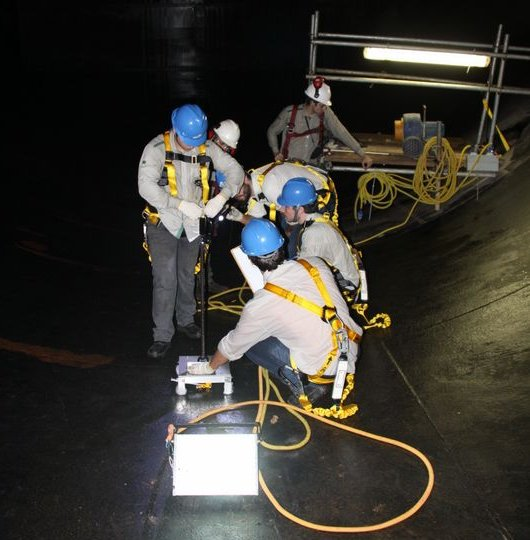
\includegraphics[width=0.6\columnwidth]{figs/base}
\caption{Teste de campo com a base  magnética}
\end{figure}

\noindent
\textbf{3500 Realização dos testes destrutivos – 1}
Realização dos testes para verificar se o revestimento mantém as 
características técnicas exigidas para a aplicação após mudanças de parâmetros. Nessa etapa foram realizados os testes de qualificação dos revestimentos antes e após mudanças de parâmetros e realização de ensaios destrutivos comparativos normatizados. 

\noindent
\textbf{3600 Aperfeiçoamento da solução:}
Aperfeiçoamento da solução baseado nos resultados dos testes de campo 

Tarefa atrasada em 1 mês com impacto de atraso de 1 mês no projeto. O cálculo da
posição relativa entre o robô e a pá, baseado em dados reais do sensor de
metrologia testado em campo, está com um erro de 0,1-0,2 graus o que resulta em
um erro de posição da extremidade do manipulador na ordem de centímetros. A
ordem de grandeza desejada para poder fazer reparo do perfil hidráulico é em
milímetros. Logo, as técnicas de alinhamento continuando sendo aprimoradas.

\begin{figure}\centering
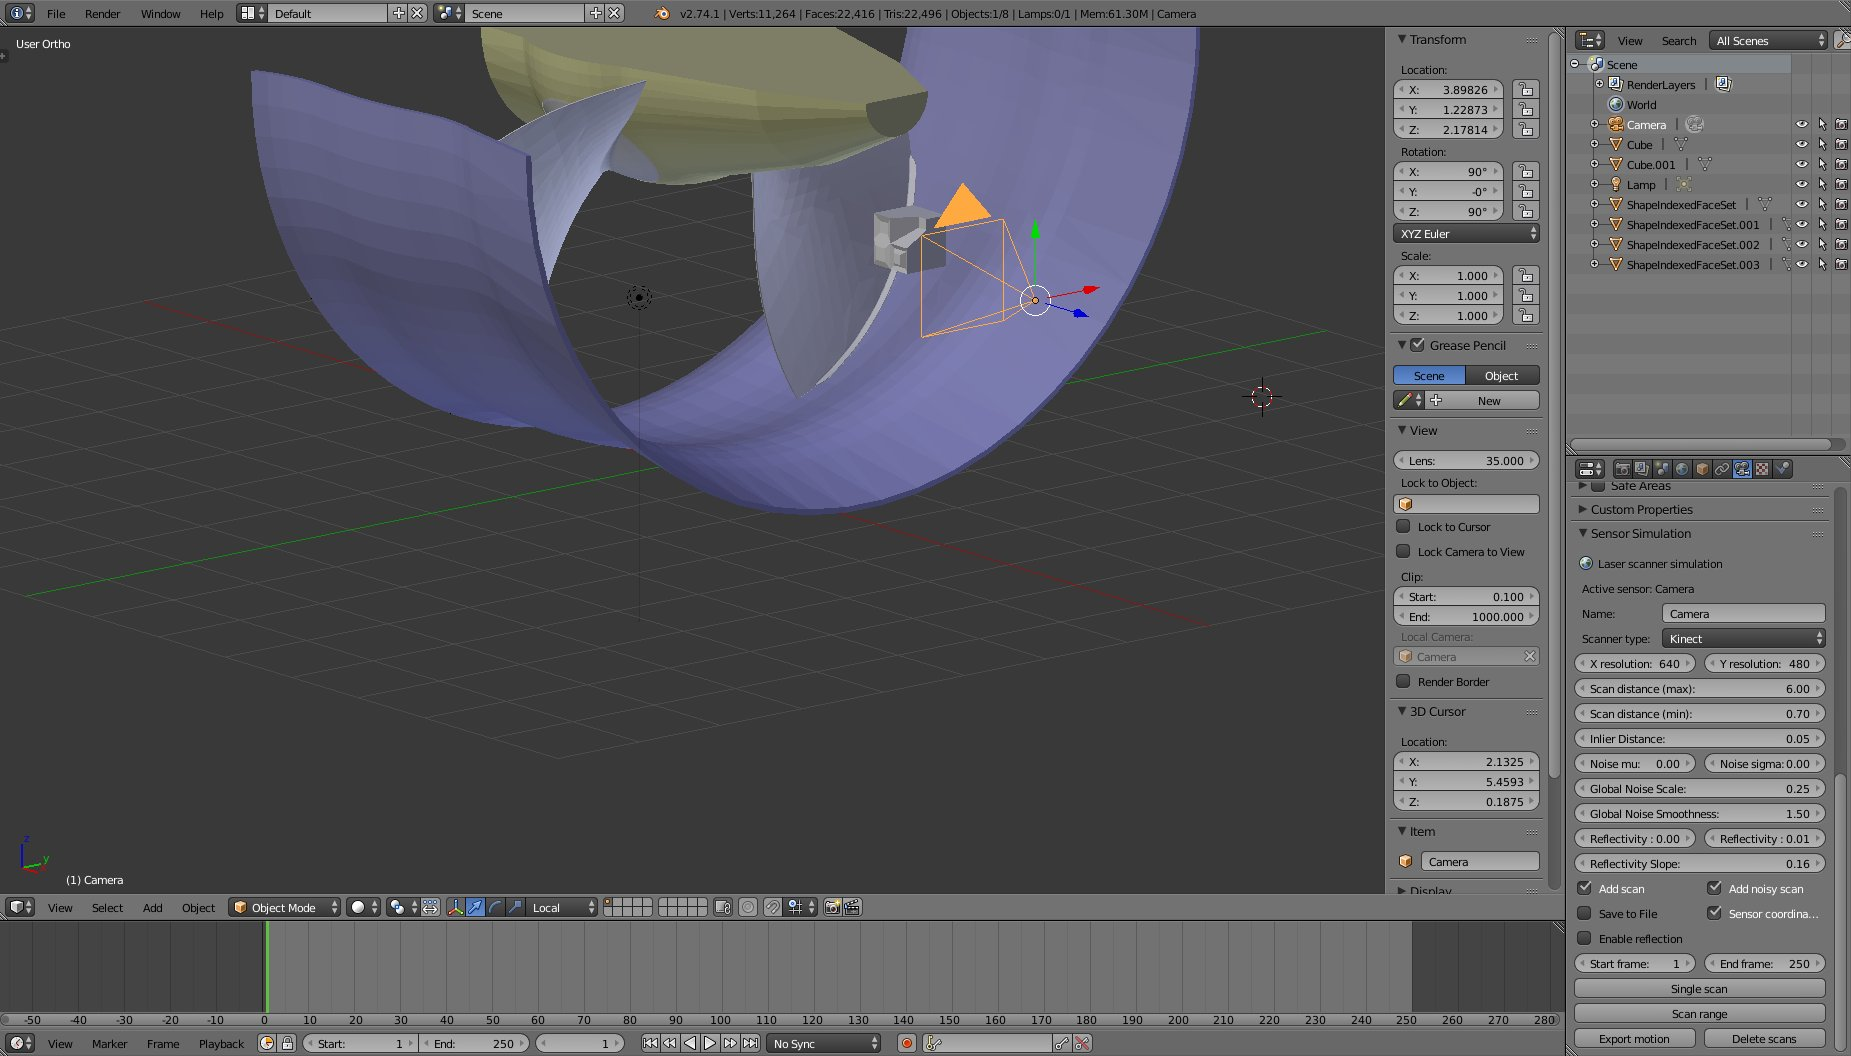
\includegraphics[width=0.6\columnwidth]{figs/blensor_screen}
\caption{Estimando posição relativa usando um simulador para análise dos
resultados.}
\end{figure} 


\noindent
\textbf{3700  Visita a campo para Inspeção 4:}
A inspeção nas pás é realizada com o fim de avaliar o progresso do desgate nas superfícies das pás e também determinar o tipo e a severidade em cada região da pá. 

\noindent
\textbf{3800 Realização dos testes destrutivos 2:}

Continuação da realização dos testes destrutivos após anális dos resultados prévio. As amostras que estvam em atraso na antrega dos resultados de cavitação foram realizadas nessa etapa. Também foram testes de aplicação de revestimento orgânico para melhoria das características do revestimento.


\noindent
\textbf{3900 Teste de Campo Jirau 02:} Teste da solução  em Jirau sobre
condições reais de operação.

Tarefa cancelada. As informações necessárias para esta fase do
projeto foram coletadas durante o teste de campo 01. 

\section{Etapa 04} 

\begin{figure}[H]
\centering
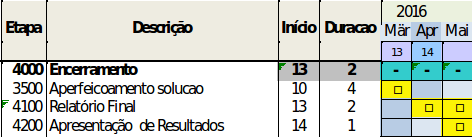
\includegraphics[width=0.7\columnwidth]{figs/etapa4}
\end{figure} 

\noindent
\textbf{4000 Encerramento:} A etapa 4000 do projeto foi executada existindo
variações entre previsto e executado. Inicialmente esta etapa era para ser
iniciada em março e encerrada em abril. Entretanto a mesma sofreu um atraso de 1
mês devido a necessidade de mais tempo para encerrar a etapa de aperfeiçoamento
da solução. O objetivo da etapa é preparar os relatórios finais e artigos acadêmicos do projeto.

\noindent
\textbf{4100 Relatório Final:} Relatório de encerramento do projeto no formato
P\&D Aneel e artigos acadêmicos.

Etapa executada como prevista. 

\noindent
\textbf{4200 Apresentação dos resultados:} Difusão dos conhecimentos.

Etapa executada como prevista. Foi realizado um evento na faculdade de Porto
Velho, onde os pesquisadores do projeto EMMA realizaram uma aula de pesquisa
aplicada explicando as pesquisas desenvolvidas, seus conceitos e resultados.
 

\chapter{Estudo do conceito}\label{cap::sota}
\section{Introdução}
O Brasil é um dos países mais ricos do mundo em recursos hídricos, facilitando o
desenvolvimento e investimento em geração de energia a partir desse recurso. A
energia hidráulica é a mais dominante em todo o país, e o Brasil é o segundo
país com maior consumo de energia hidrelétrica no mundo com capacidade
instalada de 70.000 MW, 433 usinas hidrelétricas em
operação\footnote{International Energy Agency (2010), http://www.iea.org/.}.

Estima-se que a reforma e melhoria das grandes usinas construídas resultariam
em um aumento potencial de 32.000 MW \citep{goldemberg2007energia},
número que pode ser alcançado, em grande parte, pela manutenção das turbinas
geradoras da energia elétrica. As turbinas estão constantemente expostas aos
fenômenos de abrasão e cavitação, os quais determinam sua vida útil.

O fenômeno de cavitação está muito bem estudado e detalhado em
\cite{escaler2006detection}, onde são apresentadas seus tipos, ocorrências e os
efeitos nas diferentes turbinas. Esse fenômeno físico pode causar erosões na
máquina hidráulica (figura~\ref{fig::cavitacao}), gerando instabilidade de fluxo
de água, vibrações excessivas e redução da eficiência da turbina.

\begin{figure}[h!]
	\centering	
	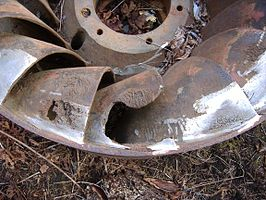
\includegraphics[width=0.7\columnwidth]{sota/figs/intro/cavitacao}
	\caption{Ilustração de uma pá de turbina que sofreu erosão por cavitação.}
	\label{fig::cavitacao}
\end{figure}

A fim de reduzir o desgaste da pá contra cavitação ou abrasão e aumentar a sua
vida útil, utiliza-se a técnica de revestimento por asperção térmica, que pode ser comparada com uma
tinta que protege à exposição com o ambiente. O procedimento é realizado
antes da instalação das pás na turbina por um robô, pois exige alta precisão
e velocidade, além de expelir substâncias nocivas à saúde. Apesar de suficiente para a proteção da pá, o
revestimento também tem vida útil e precisa ser refeito de tempos em tempos para
garantir a proteção da pá contra os fenômenos físicos.

No caso específico da usina hidrelétrica de Jirau, construída no rio Madeira,
os fenômenos de abrasão são intensos devido ao grande número
de partículas que o rio carrega diariamente, reduzindo ainda mais a vida útil do
revestimento.
Portanto, há a necessidade de manutenção regular, o que, na situação atual,
exige paralização da máquina, desmontagem da turbina, posicionamento de cada pá
na área designada ao revestimento, aplicação do revestimento, montagem da
turbina e recalibração. O tempo de paralização para a realização de
toda a manutenção pode levar de um a dois meses, significando uma grande perda
na geração de energia. 

A primeira etapa do projeto EMMA, pesquisa e desenvolvimento
realizados pela Fundação COPPETEC, em parceria com a empresa Rijeza, ANEEL e
ESBR, é um estudo de viabilidade técnica de um sistema robótico para realizar
revestimento por aspersão térmica de turbinas \textit{in situ}, ou seja, dentro
do ambiente da turbina (aro câmara). O projeto tem como objetivo reduzir
significativamente o tempo de manutenção do revestimento por ser realizado no
ambiente confinado da turbina e, portanto, não havendo necessidade de sua
desmontagem.

Este capítulo está dividido da seguinte forma: a seção 2 descreve
detalhadamente o problema, contextualiza o leitor no ambiente da usina de
Jirau e descreve as possíveis tarefas do robô; a seção 3 faz um levantamento do
estado da arte; a seção 4 descreve os projetos conceituais para o robô; e a
seção 5 conclui e descreve os próximos passos para o projeto EMMA. 



 
\section{Descrição do problema}\label{sec::consideracoes}

O fenômeno de cavitação e abrasão em hidroturbinas provoca desgaste
superficial por erosão e alteração do perfil
hidráulico da pá, gerando redução da eficiência na geração de energia.
Uma solução preventiva é o revestimento por metalização das pás, o qual aumenta a eficiência na
geração de energia por gerar uma estrutura mais lamelar, e fornece maior
resistência a desgastes. No caso da usina hidrelétrica de Jirau, o revestimento
das pás é realizado antes da montagem e instalação da turbina, porém devido ao grande número de
partículas e sedimentos que o rio madeira carrega e à cavitação, o revestimento
deve ser aplicado novamente em intervalos curtos de tempo
\citep{santa2009slurry}. A desmontagem da turbina, aplicação de novo
revestimento nas pás e remontagem são um processo muito custoso e deverá ser
feito regularmente. Portanto, há a necessidade de o procedimento ser
executado dentro do aro câmara, \textit{in situ}, onde as pás são instaladas.

A cavitação é a formação de cavidades de vapor (bolhas), em um líquido, devido a
quedas repentinas de pressão. Quando o líquido é sujeito ao aumento de pressão,
as bolhas implodem, ocasionando ondas de choque \citep{brennen2013cavitation}.

Em hidroturbinas, o fenômeno de cavitação é comum próximo às pás ou
na saída da turbina. O líquido apresenta a combinação
de componentes cinético, potencial gravitacional e energia de fluxo. O
componente cinético é em virtude do fluxo da água (velocidade), o potencial tem
relação com a altitude, e a energia de fluxo é energia que um fluido contém
devido à pressão que possui. De acordo com o princípio de Bernoulli, o princípio
da conservação para os fluidos, implica-se que, para uma mesma altitude, o
aumento da componente cinética acarreta em uma diminuição da pressão, ocorrendo
cavitação. 

Quando há cavitação, a formação de bolhas grandes altera as características do
escoamento, ocasionando oscilações ou vibrações na máquina que, por
conseqüência, prejudicam o rendimento do sistema hidráulico. As bolhas
pequenas, ao colapsar, geram ondas de choque de alta frequência, podendo provocar erosões se
próximo à superfície metálica.

Além da cavitação, como a água atravessa o aro câmara em grande velocidade, o
acúmulo de sedimentos irá provocar desgaste abrasivo, isto é, perda de material
pela passagem de párticulas rígidas. 

Nesta seção, são apresentadas as formas de reduzir os danos da cavitação pela
tecnologia de revestimento por metalização, a contextualização do problema no
caso da usina hidrelétrica de Jirau e as tarefas que um sistema robótico deve
realizar para solucionar o problema.


\subsection{Descrição do processo HVOF}\label{sec::desc_hvof}
O revestimento por aspersão térmica (ou metalização) é um processo em que
partículas aquecidas são pulverizadas em uma superfície a fim de melhorar ou
restaurar suas propriedades e dimensões. O revestimento estende a vida útil do
material, aumentando significantemente a sua resistência à erosão e corrosão.
Os diferentes tipos de metalização são: por chama, arco elétrico, detonação,
chama de alta velocidade (HVOF), plasma, a frio e a quente.

Um sistema de metalização é composto por: uma pistola de aspersão, responsável
pelo derretimento e aceleração das partículas a serem depositadas na
superfície; um alimentador, que fornece o pó (partículas) através de tubos;
um fornecedor do material de combustão; um robô para manipular a pistola; uma
fonte de alimentação elétrica para a pistola; um console de controle para o
sistema.

No caso específico das pás (aço inox 420) das turbinas da usina hidrelétrica de
Jirau, antes da montagem da turbina, a metalização tipo HVOF é realizada em
ambos os lados da pá pela empresa RIJEZA com um manipulador industrial de 150 kg
de carga máxima, permitindo controle de vibrações com boa margem de segurança, já que a massa do
sistema pode chegar a 10 kg (cabos e pistola). O tempo
mínimo do processo é de 6 horas por lado da pá.

O HVOF consiste em alimentar, numa câmara de combustão, o material de
revestimento (carboneto de tungstênio), uma mistura gasosa do combustível (propano) e
oxigênio. De acordo com os dados fornecidos pela empresa RIJEZA, a pistola de 8
Kg projeta uma chama de $3000^oC$, que pulveriza as partículas com velocidade de
700 a 1000 m/s, gerando uma força de recuo de 15 N.

O manipulador robótico deve possuir precisão de 5 mm, a pistola no efetuador
deve permanecer a uma distância que varia entre 230 e 240 mm, e ângulo de $90^o
\pm 60^o$, em relação à superfície. O manipulador deve ser capaz de
mover a pistola a velocidade constante de 40 m/min, e não pode permanecer uma
posição da pá por muito tempo (parada), pois há acúmulo de material, deformando a
superfície. Trocas de direção ou sentido na movimentação do manipulador são
considerados como parada, logo as trocas deverão ser realizadas em áreas
exteriores à superfície da pá ou chapas de sacrifício são utilizadas. 

Placas de sacrifício, ou mascaramento, são chapas colocadas em regões onde as
peça não podem ser jateadas ou revestidas. Geralmente uma chapa de qualquer tipo
de aço pode ser utilizada, pois a chama não fica parada sobre ela por um longo
período, não aquecendo-a o suficiente para danificar. Quando a pistola
permanece, em funcionamento, a chama é apontada para algum lugar onde não tenha obstáculos.

 % As informações do processo
% podem ser observadas na figura~\ref{fig::hvof}.
 
%\begin{figure}[h!]	
%	\includegraphics[width=\columnwidth]{sota/figs/intro/hvof.pdf}
%	\caption{Foto do efetuador do manipulador e pistola HVOF.}
%	\label{fig::hvof}
%\end{figure}

Em relação às condições de operação: o espaço da aplicação HVOF é confinado,
com excesso (100 a 140 dB), gases nocivos e com risco de explosão podem
ser exalados; a pá pode atingir temperaturas de até $110^oC$; as condições de
umidade e temperatura devem ser ideais para o processo; e há perda de $40\%$
das partículas pulverizadas  \citep{wu2006rebound}, que são espalhadas pelo
ambiente. Portanto, algumas medidas devem ser tomadas para a execução do
processo: a operação deve ser remota, não há presença de pessoas \textit{in
loco}; os gases presentes e umidade/temperatura devem ser constantemente
monitorados; o robô manipulador é selado; as partículas desperdiçadas devem
ser removidas (limpeza); e o desligamento do sistema deve ser acompanhado por corte de gás.

A qualidade do revestimento é geralmente avaliada por um instrumento que
realiza a medida de porosidade, oxidação, dureza e rugosidade da superfície. O
processo é realizado manualmente, de maneira rápida e fácil, por um operador.

A tabela~\ref{tab::hvof} resume as restrições e especificações do
projeto:

\begin{center}
\begin{tabular}{  c | c  }
  \hline
  \textbf{Componente} & \textbf{Dado} \\ \hline
  Massa da pistola HVOF & 8 Kg  \\ \hline
  Massa dos cabos HVOF & 12 Kg  \\ \hline
  Tempo HVOF por pá & 6 horas \\ \hline
  Temperatura da chama HVOF & $3000^oC$ \\ \hline
  Recuo da pistola & 15 N \\ \hline
  Precisão do manipulador & 5 mm \\ \hline
  Distância pistola-pá & 230-240 mm \\ \hline
  Ângulo pistola-pá & $30^o$-$90^o$ \\ \hline
  Velocidade do manipulador & 40 m/s \\ \hline
  Ruído HVOF & 100 a 140 dB \\ \hline
  Temperatura da pá & $110^oC$ \\
  \hline
\end{tabular}
\captionof{table}{Dados principais do processo HVOF}
%\caption{Dados principais do processo de metalização HVOF}
\label{tab::hvof}
\end{center}

%Sistemas robóticos não devem utilizar magnetismo como meio de aderência, já que
%o aço inox 420 não apresenta alta permeabilidade magnética e a alta temperatura
%da pá deve inviabilizar essa solução. Adesão por ventosas é uma solução
%viável, pois material não causa dano ao revestimento, porém a escolha do
%material da ventosa deve ser estudado,já que a pá quente pode ocasionar em
%perda de sucção, como em ventosas emborrachadas.


\subsection{Descrição dos requistios de operação de HVOF}

O processo de metalização de turbinas hidrelétricas tem alguns pré-requisitos
que devem ser respeitados para uma correta aplicação e fixação da camada de
material durante o revestimento. Essa subseção descreverá as etapas necessárias
de preparação da superfície a fim de se assegurar a manutenção da qualidade dos resultados e do
perfil hidráulico da pá. 

\subsubsection{Jateamento da superfície da pá}\label{sec:jat}

O processo de metalização sobreposto a uma superfície que já possui uma camada
protetora desgastada não apresenta um resultado tão satisfatório se comparado
com o processo realizado em uma superfície crua. Por esse motivo é recomendado
que seja realizado um processo de jateamento abrasivo. 

O jateamento consiste em direcionar um fluxo de material abrasivo na superfície
do material a fim de se erodir a mesma e retirar o material depositado na camada
superficial. Outra característica desse processo é a capacidade de aumentar a
rugosidade da superfície e, assim, aumentar o poder de adesão da nova camada a
ser metalizada.  

O processo de jateamento para o tratamento específico da superfície das pás da
turbina utiliza óxido de alumínio como material abrasivo e pode ser realizado
por um operador. A infraestrutura necessária para esse processo é uma fonte de
ar comprimido, geralmente proveniente de um compressor de ar, para propulsionar
o particulado que forma o jato abrasivo. %\textbf{A preparação do ambiente no
% envolto da pá, o escoamento do material e
%as consequências da realização desse processo não foram analisados} e,
%possivelmente, será necessária a implementação de infraestrutura de suporte
%para proteção dos equipamentos adjacentes que não receberão o jateamento,
%limpeza do material depositado e exaustão do particulado suspenso.

\subsubsection{Reparo de danos existentes}

Danos existentes na superfície da pá ou em sua estrutura podem reduzir a sua
eficiência e até mesmo a própria integridade da pá, prejudicando a segurança 
da operação. O processo de metalização não tem a capacidade de reparar
danos severos na superfície ou danos estruturais como rachaduras. A inspeção
para procura desses defeitos deve ser realizada antes da realização do processo
de metalização, uma vez que a superfície jateada, ou seja, em metal cru sem
camada de proteção, facilita a visualização de danos. %Os procedimentos para
%reparos de danos estruturais ou referentes a rachaduras não serão cobertos por
%este documento.

Os danos causado por cavitação, como explicado na seção
\ref{sec::consideracoes}, pode alterar o perfil hidráulico da pá e deve ser
reparado sempre que possível. O procedimento de reparo varia de acordo com a
severidade dos danos causados. À medida que a profundidade das cavidades geradas
na pá e a extensão dos danos vão aumentando, medidas mais extremas se tornam
necessárias e, por isso, a estratégia de reparo para esse tipo de dano deve
estar alinhada com o tipo de processo que se deseja utilizar. Inspeções e
reparos mais frequentes significam processos mais simples, enquanto que reparos
mais espaçados podem resultar até na inutilização da pá. Os procedimentos mais
utilizados para o reparo de danos causados por cavitação são:

\begin{itemize}
  \item Reparo com materiais não fundidos à superficie;
  \item Reparo por solda;
  \item Reparo por solda e placa sólida.
\end{itemize}

\paragraph{Reparo com materiais não fundidos à superficie}
Para pequenos danos, é possível utilizar processos nos quais não é necessário
fundir o material depositado para preenchimentos das cavidades ao material da
superfície metálica da pá. Os processos e materiais utilizados, usualmente na
indústria, são: 

\begin{itemize}
\item Epoxy;
\item Cerâmica;
\item Revestimento por metalização;
\item Neoprene;
\item Urethane.
\end{itemize}

Vale ressaltar que a solução proposta para a metalização de uma camada protetora
para se evitar os danos causados pela cavitação também poderia ser utilizado
para preencher danos passados, desde que respeitem o limite de espessura
para o tipo de processo utilizado


\paragraph{Reparo por solda}

O preenchimento dos danos causados devido à cavitação por solda é o procedimento
mais comum, pois possibilita uma maior deposição de material e não obriga a
realização de reparos com uma frequência elevada. Esse processo consiste na
deposição de solda em camadas, até o completo preenchimento. A
superfície deve ser, então, esmerilhada até entrar em conformidade com as
medidas padrão de qualidade para o perfil hidráulico da pá a ser reparada. Essa tarefa
é normalmente realizada por mão de obra altamente qualificada e existe, também,
na literatura a presença de soluções automatizadas, como os robôs Roboturb e Scompi
\citep{roboturb,scompi}

\paragraph{Reparo por solda e placa sólida}

Para casos de danos mais severos, pode ser necessária a utilização de placas
para o preenchimento de grandes extensões. O processo de fixação das placas é
realizado por solda, assim como o preenchimento do volume restante. O processo
de solda, esmerilhamento e verificação é comum ao procedimento padrão utilizando
somente solda.
















\subsection{Contextualização do Ambiente}\label{sec::desc_contex}

A usina hidrelétrica Jirau é do tipo fio d'água, na qual são utilizadas turbinas
do tipo bulbo de eixo horizontal. Como a geração de energia depende da altura da queda d'água e da vazão do rio, as turbinas do tipo bulbo utilizam uma grande vazão de
água para produzirem energia elétrica suficiente. A figura
\ref{fig::bulb_turbine} e a tabela \ref{tab::bulb_turbine} ilustram uma turbina
do tipo bulbo e o grandes dutos necessários para comportar o grande volume de água que passa através da turbina. 
 
\begin{figure}[h!]	
	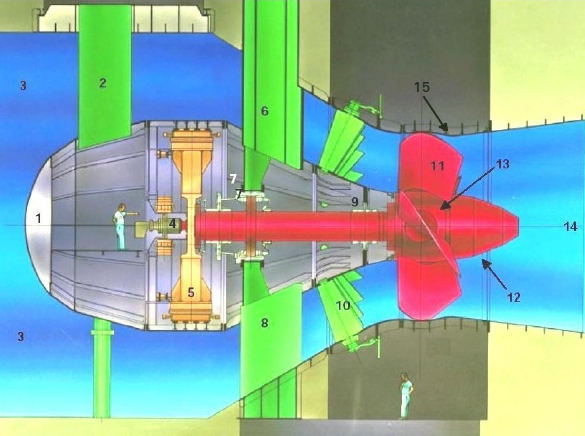
\includegraphics[width=\columnwidth]{sota/figs/intro/bulb_turbine2}
	\caption{Ilustração de uma turbina do tipo bulbo.}
	\label{fig::bulb_turbine}
\end{figure}

\begin{center}
\begin{tabular}{  c | c  }
  \hline
  \textbf{Número} & \textbf{Componente} \\ \hline
  1 & Nariz do bulbo \\ \hline
  2 & Tubo de acesso ao gerador  \\ \hline
  3 & Câmara de adução  \\ \hline
  4 & Cabeçote Kaplan  \\ \hline
  5 & Gerador Síncrono  \\ \hline
  6 e 8 & Estrutura de sustentação \\ \hline
  6 & Tubo de acesso à turbina \\ \hline
  7 e 9 & Mancais Combinado e Guia \\ \hline
  10 & Distribuidor \\ \hline
  11 & Pás do Rotor \\ \hline
  12 & Cone ou Ogiva \\ \hline
  13 & Cubo \\ \hline
  14 & Tubo de sucção/descarga \\ \hline
  15 & Aro Câmara \\
  \hline
\end{tabular}
\captionof{table}{Componentes principais de uma turbina tipo bulbo}
%\caption{Componentes principais de uma turbina tipo bulbo}
\label{tab::bulb_turbine}
\end{center}



Atualmente, caso seja necessário algum reparo ou inspeção na turbina, é necessário que se interrompa o fluxo de água e que 
toda a água em seu interior seja drenada. Para manutenção do rotor, existe uma escotilha de acesso de diâmetro limitado. Entretanto, caso deseje-se realizar 
a metalização de pás já instaladas, utilizando-se os processos atuais, é
necessária a retirada de todo o aro câmara, desmontagem completa do rotor e logística de transporte das pás até o local
onde a metalização será realizada. Essa operação, caso necessite ser realizada, demandaria a mobilização
de diversas equipes de manutenção, operação de pórtico rolante e transporte,
além de impossibilitar a utilização da turbina durante várias semanas.
No contexto da solução proposta, os pontos de interesse da turbina são:

\begin{itemize}
  \item Hélice e pás;
  \item Aro Câmara e regiões adjacentes;
  \item Escotilhas de acesso;
  \item Tubo de Sucção;
  \item Infraestrutura disponível
\end{itemize} 

\subsubsection{Hélice e pás}
 
O rotor ou hélice da turbina é constituído do cubo, as pás e o cone. 
Nas turbinas da usina Jirau, cada pá mede, aproximadamente, 2,5m de altura e
3m de largura. A partir do interior da turbina, todas as superfícies da pá são
alcançáveis, com exceção da borda e do lip da pá. O único ponto de acesso à
essa regiâo é por meio da escotilha superior de acesso. A figura
\ref{fig::blade_rijeza} exemplifica uma pá do rotor presente na usina Jirau recém metalizada no galpão da Rijeza.

\begin{figure}[h!]
	\centering	
	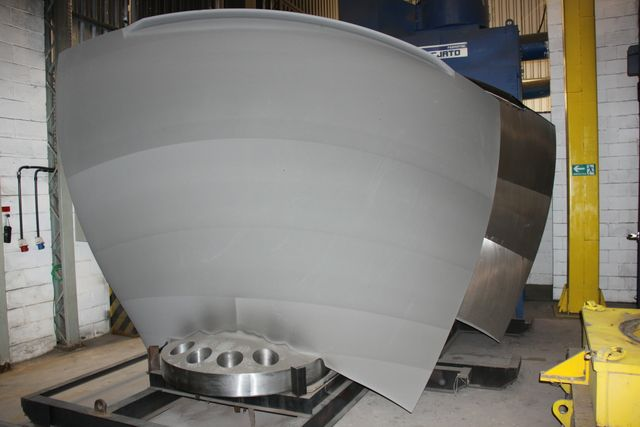
\includegraphics[width=0.7\columnwidth]{sota/figs/viagem/img_4887}
	\caption{Pá do rotor recém metalizada.}
	\label{fig::blade_rijeza}
\end{figure}

A angulação de cada pá em relação ao fluxo d'água pode ser alterado em 29$^o$,
14.5$^o$ para cada lado a partir da posição inicial, não havendo sobreposição
entre as pás, como ilustrado na figura \ref{fig::blades_angle}.
Essa angulação pode ser explorada para otimizar o espaço de trabalho necessário
para o processamento da pá e também influencia o acesso à região
entre o distribuidor e o rotor, uma vez que não existe acesso pela montante da
turbina. Entretanto, vale observar que esta angulação não pode ser alterada
manualmente e só pode ser realizada uma vez, antes do desligamento da turbina. A
posição do rotor também pode ser manualmente alterada, possibilitando que o mesmo seja girado em ambas as direções e sem limite de revoluções. Entretanto, essa operação é uma tarefa imprecisa e envolve um certo risco às pessoas que a realizam. Sendo
assim, a solução proposta deve otimizar o número de rotações necessárias para o processamento de todas as pás.

\begin{figure}[h!]	
	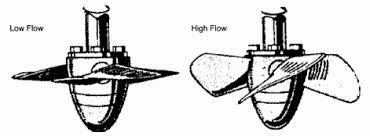
\includegraphics[width=\columnwidth]{sota/figs/intro/blades_angle}
	\caption{Exemplo de limites de rotação das pás do rotor.}
	\label{fig::blades_angle}
\end{figure}

\subsubsection{Aro Câmara e regiões adjacentes}

O aro câmara, assim como o a região próxima ao distribuidor e também ao tubo de
sucção possuem superfícies metálicas. Essa característica possibilita a
exploração de soluções de fixação magnética.

Somente a região compreendida pelo aro câmara é plana e tendo como agravante a presença do distribuidor na região à 
montante ao rotor. É necessário que a inclinação presente nessas superfícies seja contabilizada e uma solução eficiente 
de apoio ou plano elevado seja desenvolvida caso haja necessidade de fixação de alguma parte do sistema. Atualmente todo 
o trabalho é realizado por meio da montagem de andaimes ancorados por cordas. %A
%figura \ref{fig::andaime} ilustra uma estrutura utilizada no modo de inspeção e
%manutenção atuais.

%\begin{figure}[h!]	
%	\centering
%	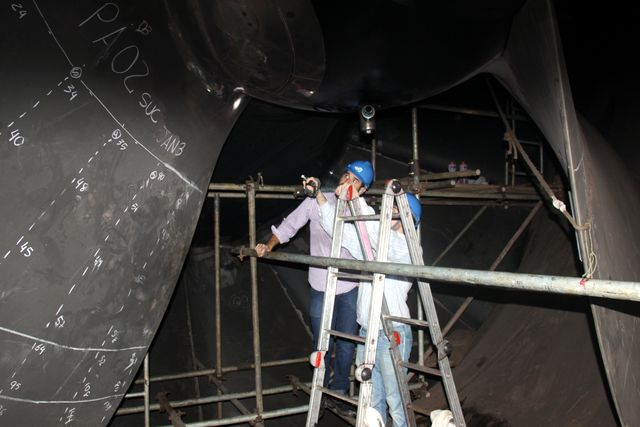
\includegraphics[width=0.8\columnwidth]{sota/figs/viagem/img_4969}
%	\caption{Andaime montado no interior da turbina e ancorado por cordas}
%	\label{fig::andaime}
%\end{figure}

 
\subsubsection{Escotilhas de acesso}
O acesso à turbina se dá por duas escotilhas, uma inferior, localizada no ínicio do tubo de sucção 
próxima ao aro câmara e outra superior, localizada na parte superior do aro câmara.

A escotilha inferior, ilustrada na figura \ref{fig::esc_inf} é o acesso
utilizado para a entrada de pessoas na turbina e todo material utilizado para reparos é transportado através dessa escotilha. Na usina Jirau existem dois 
tipos de escotilha de acesso inferior, sendo a menor delas possuindo 80cm de diâmetro. 

A escotilha superior é utilizada, principalmente, para a inspeção visual do
estado dos Lips das pás.
O diâmetro do acesso superior é de aproximadamente $35.7cm$, limitando as
dimensões dos equipamentos que podem ser transportados através da escotilha. As figuras \ref{fig::esc_sup_ext} e
\ref{fig::esc_sup_int} ilustram o acesso à escotilha superior pelo exterior ao
aro câmara e a visão pelo interior da turbina,
respectivamente.

\begin{figure}[h!]	
	\centering
	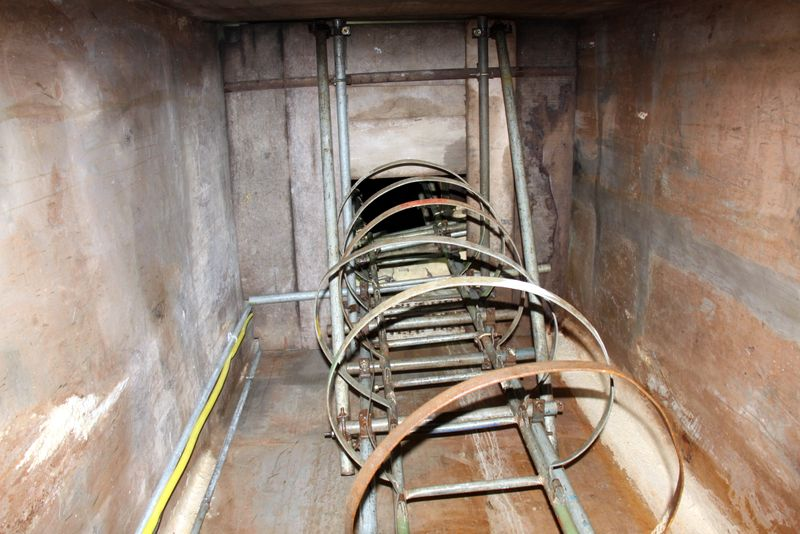
\includegraphics[width=0.8\columnwidth]{figs/esc_inf}
	\caption{Vista exterior da escotilha inferior.}
	\label{fig::esc_inf}
\end{figure}




\begin{figure}[h!]	
	\centering
	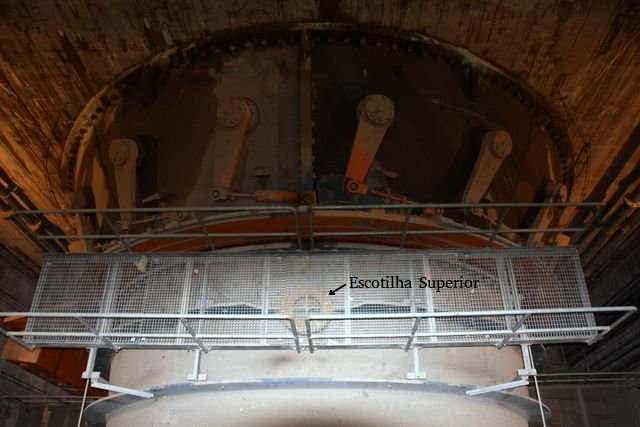
\includegraphics[width=0.8\columnwidth]{sota/figs/viagem/img_4979_mod}
	\caption{Vista da escotilha superior pelo exterior do aro câmara}
	\label{fig::esc_sup_ext}
\end{figure}

\begin{figure}[h!]	
	\centering
	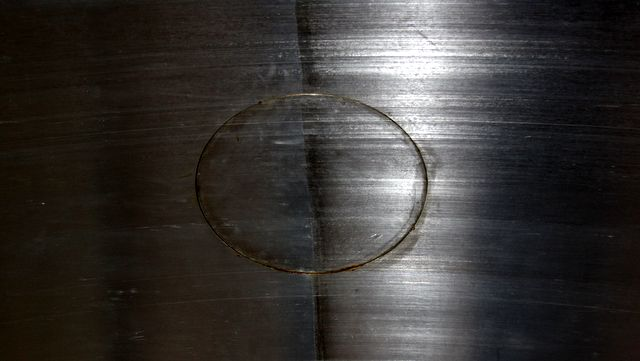
\includegraphics[width=0.8\columnwidth]{sota/figs/viagem/img_4982}
	\caption{Vista da escotilha superior pelo interior do aro câmara}
	\label{fig::esc_sup_int}
\end{figure}

\subsubsection{Tubo de sucção}

Ao final do tubo de descarga está localizado o vão dos stoplogs 
de jusante ou da comporta vagão e, em seguida, o leito do rio, como ilustrado
na figura \ref{fig::tubo_suc}.
Caso os stoplogs não estejam inseridos, existe um vão de, pelo menos, 10 m de largura. Porém, não
é válida a utilização deste vão como acesso à turbina, pois há grande fluxo de
água devido à abertura do distribuidor. O distribuidor não é fechado
imediatamente por questões ambientais, já que este é o escoamento de peixes.

%criando assim
%um acesso extra para um sistema submarino. A figura \ref{fig::tubo_suc}
%exemplifica a magnitude do tamanho do acesso, deixando claro que o limitante de
%tamanho do sistema para a utilização desse acesso é o vão de entrada do
% stoplog, ilustrado na figura \ref{fig::stoplog}. Outra alternativa é utilizar um
%guindaste e submergir o sistema pelo próprio rio, entretanto o sistema ficaria
%sujeito as condições do ambiente.

\begin{figure}[H]
	\centering	
	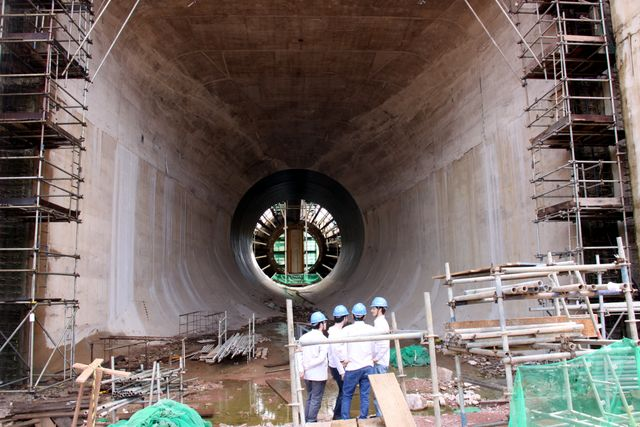
\includegraphics[width=0.8\columnwidth]{sota/figs/viagem/img_5086}
	\caption{Abertura do tubo de sucção para o leito do rio, em fase de
	construção.}
	\label{fig::tubo_suc}
\end{figure}

\subsubsection{Infraestrutura disponível}
É importante ressaltar a infraestrutura dísponível para o desenvolvimento da solução. 
Após o ensecamento da turbina, é possível a disponibilização de energia elétrica
e ar comprimo em seu interior, ambos importantes para o processo de metalização. Outro fator 
importante é a presença de um pórtico rolante que tem acesso até o andar diretamente 
inferior ao aro câmara, posicionando todo o equipamento necessário nas proximidades 
da escotilha de acesso inferior. É possível também o acesso direto, por meio de pórtico, 
à escotilha superior.

\begin{figure}[h!]	
	\centering
	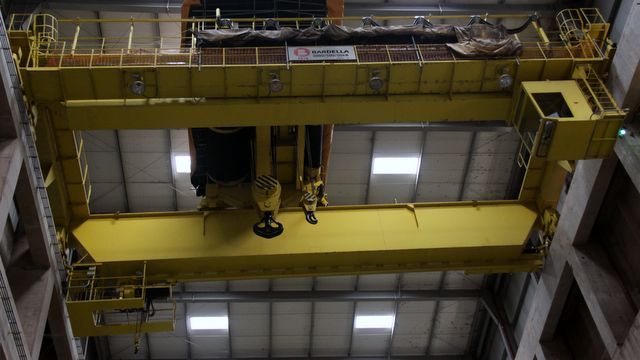
\includegraphics[width=0.8\columnwidth]{sota/figs/viagem/img_4989}
	\caption{Pórtico rolante com acesso ao exterior do aro câmara}
	\label{fig::portico}
\end{figure}


O ambiente pode ser resumidamente caracterizado pelas dimensões das pás,
elemento a ser processado; características do aro câmara, estrutura que limita o
espaço de trabalho do robô; e pelos acessos nos quais o sistema terá que
utilizar:

\begin{itemize}
  \item \textbf{Pás do rotor} - Material aço inox 420. Dimensões 2.5 x 2.5 m de superfície;
  \item \textbf{Aro Câmara} - estrutura cilíndrica com raio de 3.95 m e
  superfície metálica;
  \item \textbf{Acessos}: 
  	\begin{itemize}
    	\item Escotilha superior - 35 cm de diâmetro;
  		\item Escotilha inferior - 80 cm de diâmetro;
  		\item Tubo de descarga - 20 x 20 m, porém acessado pelo rio. 
  	\end{itemize}
\end{itemize}







\subsection{Descrição das tarefas do robô}
\label{desc_taref}
Esta subseção descreve as tarefas básicas do robô para o revestimento de
turbinas \textit{in situ}. Em linhas gerais, o robô a ser desenvolvido deve ser
capaz de realizar a tarefa de revestimento tal qual seria feita caso a pá não estivesse instalada na
tubina e de uma maneira autônoma. A pá, antes de ser submetida ao
processo de revestimento, deve estar em conformidade com o gabarito, perfil hidráulico de uma pá
intacta. Portanto, uma tarefa do robô é realizar o mapeamento do perfil
hidráulico, construir um modelo 3D e analisar imperfeições.

Em caso de deformações, causados por cavitação e abrasão, estas precisam
ser removidas manualmente ou de forma automatizada, possivelmente por
soldagem. A tarefa de soldagem pode
ser realizada por operador, manualmente, por não possuir todas as restrições
da tarefa de revestimento (velocidade, precisão, carga e etc), porém o ambiente
pode dificultar a operação de forma que a execução por um robô seja
indispensável. 

Após as pás estarem de acordo com o gabarito, faz-se a
identificação do desgaste do revestimento, medindo sua espessura em pontos
pontos específicos sobre a superfície da pá. Manualmente esse
processo é realizado eficientemente em 10 min, justificando a não necessidade de
esta ser uma tarefa do robô. 

Em caso de necessidade de aplicação
de novo revestimento, é necessária a remoção do revestimento antigo por
jateamento, a fim de deixar a superfície rugosa e aumentar sua aderência. A
tarefa de jateamento é atualmente realizada maualmente, mas também pode ser
realizada pelo robô. Como ambos os lados da pá são revestidos, o jateamento deve
ser realizado em ambos os lados. Vale ressaltar que, em teoria, pode-se aplicar revestimento por metalização sem retirar o último revestimento,
porém esse processo ainda se encontra em fase de estudos na Rijeza.
%Segue-se o exemplo de empresas de aviação, onde existe a
%prática de retirar todo o revestimento antigo antes de aplicar o novo.

Por fim, o robô deverá aplicar o revestimento como
forma de prevenir o dano causado pelos fenômenos abrasivos. O robô projetado
para fazer o revestimento precisa preencher todos os requisitos discutidos na
subseção~\ref{sec::desc_hvof} e ser adaptável ao ambiente, cujos as restrições
são discutidos na subseção~\ref{sec::desc_contex}. 

Das tarefas a serem relizadas, são destacadas as seguintes:

\textbf{Tarefas que podem ser executadas manualmente:}
\begin{itemize}
  \item Inspeção e análise de danos na pá, tanto para reparo quanto para
  revestimento;
  \item Reparo;
  \item Montagem do sistema;
  \item Jateamento da superfície;
\end{itemize}

\textbf{Tarefas que poderão ser executadas pelo robô:}
\begin{itemize}
  \item Modelar o perfil hidráulico;
  \item Calibração;
  \item Jateamento;
  \item Reparo (soldagem e esmerilhamento);
  \item Revestimento por metalização;
\end{itemize}




\section{Estado da arte}\label{sota/sota}
 
O estudo do estado da arte de robôs para a realização de HVOF em pás de turbinas
hidráulicas contempla os sistemas que atendem a alguns dos requisitos: operar
em ambientes de alta periculosidade; capacidade de carga para os dispositivos HVOF;
manipular a pistola HVOF com velocidade de $0.67 m/s$; precisão de 5mm; ter
área de trabalho de 2.5 m x 2.5 m; e operar sob superfícies 3D de geometria
complexa. As soluções foram divididas em subseções de acordo com as tecnologias
de fixação dos robôs.


 
\subsection{Robôs sobre trilhos}
\label{sec::rail}
Na indústria, a automatização de processos de metalização, é
normalmente realizada com a utilização de manipuladores robóticos, pois oferece
a versatilidade de tarefas e espaço de trabalho necessários para esse
tipo de aplicação. Entretanto, um sistema composto por um braço robótico capaz
de operar em toda a extensão da superfície da pá da turbina hidrelétrica
não é compacto, nem móvel o suficiente para ser instalado e desinstalado para a
operação de manuntenção \textit{in-situ}.

A introdução de uma junta prismática acoplada a um trilho é uma estratégia para
reduzir o tamanho e o peso de um manipulador robótico.  Assim, é possível estender o
 espaço de trabalho do robô, sem adicionar peso ao manipulador, uma vez que o
 trilho pode usar as estruturas presentes no ambiente como apoio. 

Na literatura foram encontradas duas soluções para aplicações de manutenção e
inspeção, como solda, específicas para o contexto de turbinas hidráulicas. As
aplicações diferem, principalmente, na estratégia de fixação do sistema
de trilhos.
O Roboturb \citep{roboturb} realiza a fixação
diretamente na pá do rotor, enquanto o robô Scompi \citep{scompi} utiliza um
trilho fixado em
estruturas adjacentes à pá ou peça a ser reparada.

O Roborturb consiste em um manipulador robótico com seis juntas de revolução e
uma junta primsática acoplada a um trilho flexível, como pode ser observado
na figura \ref{fig::roboturb}, utilizado para o preenchimento de cavidades
geradas por cavitação.
O trilho pode ser conformado e, então, fixado à superfície da pá por meio de um
 sistema passivo de ventosas ou ímãs. O robô tem a possibilidade de utilizar dois 
 efetuadores distintos, o primeiro consiste em um sensor ótico para inspeção do 
 estado de erosão da pá e o segundo consiste em uma ferramenta de solda do 
tipo tocha plasma PWH-4A com alimentador automático de arame, responsável pelo 
depósito de solda para o preenchimento das cavidades identificadas pelo sistema.


%TODO Abelha: Posicionar corretamente as figuras
    \begin{figure}[h!]	
		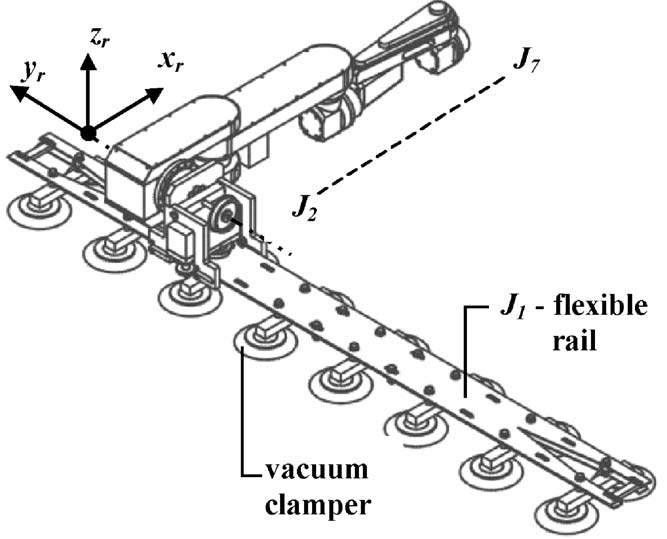
\includegraphics[width=\columnwidth]{sota/figs/trilhos/roboturbpaper}
		\caption{Roboturb - Manipulador robótico sobre trilho flexível}
		\label{fig::roboturb}
	\end{figure}
	\begin{figure}[h!]
		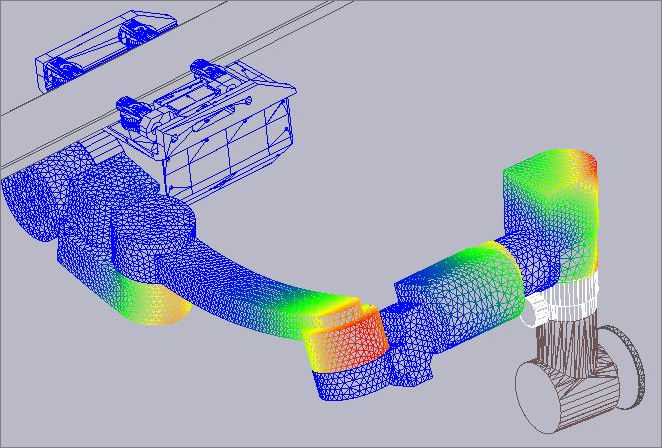
\includegraphics[width=\columnwidth]{sota/figs/trilhos/scompi}
		\caption{SCOMPI - Manipulador robótico sobre trilhos rígidos}
		\label{fig::scompi}
	\end{figure}

Por sua vez, o robô Scompi, fig \ref{fig::scompi}, é um manipulador
multipropósito projetado para realizar reparos em turbinas do tipo \textit{Francis},
 como solda e esmerilhamento das pás. O sistema possui seis graus de liberdade,
 sendo consitituído por um braço robótico com cinco juntas de revolução, e o
 último grau de liberdade proveniente de uma junta prismática que percorre um sistema de 
 trilhos retos ou curvos que são projetados para cada aplicação especificamente. 


Sistemas baseados em trilhos tem como maior benefício a redução do tamanho e,
consequentemente, do peso do manipulador necessário para a execução de tarefas
em um espaço de trabalho que englobe toda a superfície da pá.
Essa redução proporciona facilidade de transporte do robô até o interior da
turbina e também possibilita o projeto de manipuladores que tenham a rigidez
necessária para a realização das tarefas desejadas. 

Manipuladores robótico fixos, rígidos o suficiente para aguentar as forças intrínsecas ao
processo de metalização e com espaço de trabalho necessário para trabalhar em
toda a extensão da superfćie da pá seriam muito pesados.
Entretanto, sistemas baseados em trilhos com fixação na própria pá do rotor, necessitam que
o trilho seja movido caso se deseje que toda a superfície da pá sofra
manuntenção, uma vez que a área em que o trilho está apoiado não pertence ao espaço de
trabalho do robô. Em adição, sistemas com fixação de trilhos nas estruturas
adjacentes à pá devem atentar as condições para a instalação disposta pelo
ambiente para equilibrar a relação de custo benefício entre facilidade de
instalação/remoção do trilho e a robustez.

\textbf{Vantagens:}
\begin{itemize}
  \item Redução do tamanho necessário do manipulador;
  \item Redução do peso do manipulador
\end{itemize}

\textbf{Desvantagens:}
\begin{itemize}
  \item Necessidade de instalação e remoção dos trilhos;
  \item Necessidade de movimentação dos trilhos (para trilhos fixados
  diretamente nas pás)
\end{itemize}



 
\subsection{Robôs escaladores}\label{sota_climbers}
Robôs escaladores são sistemas capazes de sustentar seu próprio peso contra a
gravidade, movendo-se em simples ou complexas estruturas geométricas, como
paredes, tetos e telhados, palhetas de turbinas e plantas nucleares.
Essa classe de robôs oferece eficiência operacional em ambientes
de alta periculosidade, sendo utilizados visando saúde e segurança dos
trabalhadores, como em inspeção e limpeza de arranha-céus, diagnóstico de
tanques de armazenamento em plantas nucleares, solda e manutenção de cascos de
navios e palhetas de turbinas \citep{armada2003application}. 

Os grandes desafios nos projetos de sistemas escaladores são mobilidade e
aderência, além de consumo de energia, capacidade de carga e peso. Em
\cite{modular} e \cite{climbsurv}, os robôs escaladores são divididos em tipos
de locomoção:
pernas; como andador; utilizando segmentos deslizantes; rodas; esteiras; avanço
pendurado por braços; por cabos; e biomimética. E categorias de adesão: sucção
ou pneumática; magnética; eletrostática; química; preensão; e híbrida.

No caso específico deste estudo da arte, destacam-se os robôs escaladores com as
seguintes aplicações:

\begin{itemize}
  \item \emph{Navios e turbinas}: RRX3 para soldagem
  \citep{rrx3}, \emph{Climbing Robot for Grit Blasting} para limpeza
  \citep{crgb} e ICM Robot para inspeção \citep{icm};
  \item \emph{Industrial}: ROMA II \citep{roma} e
  CROMSCI \citep{CROMSCI}, ambos para inspeção; 
 \item \emph{Planta petroquímica}: TRIPILLAR \citep{tripillar} para inspeção.  
\end{itemize}

O RRX3 (figura~\ref{rrx3}), Daewoo Shipbuilding and Marine Engineering, é um
robô para a soldagem de casco de navios. Possui adesão por preensão, locomoção transversal utilizando segmentos deslizantes e locomoção
longitudinal por rodas. Possui um manipulador de 1.5 m com três juntas
prismáticas e três juntas de revolução (3P3R) para a operação de soldagem. 

As características principais do robô são: base e manipulador com
capacidades de carga de 120 kg e 5 kg, respectivamente; manipulador com precisão
milimétrica e efetuador de baixa velocidade; robustez para operar em ambiente de
alta periculosidade; opera instrumento de solda; e locomoção transversal é
restrita à aplicação.

\begin{figure}[ht]
\centering
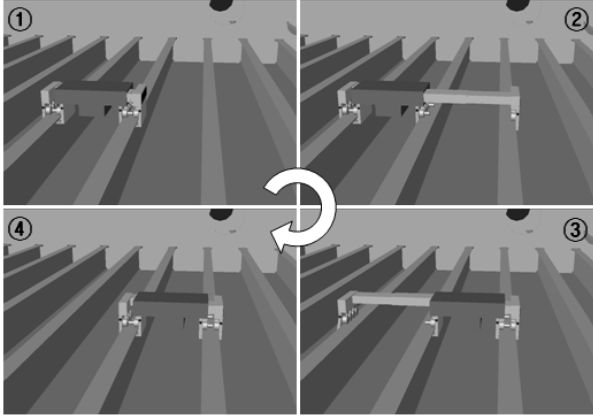
\includegraphics[width=\columnwidth]{sota/figs/climbers/RRX3_moving.jpg}
\caption{Translação horizontal do robô RRX3.}
\label{rrx3}
\end{figure}

O \emph{Climbing robot for Grit Blasting} (figura~\ref{grit}), University of
Coruna, é um robô para jateamento abrasivo em navios. O robô utiliza duas plataformas deslizantes com sistema de adesão por
ímã magnético. Os módulos apresentam movimentação relativa entre si e pode rotar
para compensar as curvaturas do casco do navio ou desviar de objetos. 

As características principais do robô são: base com
capacidade de carga de sistema abrasivo semelhante a HVOF; base com
locomoção de precisão milimétrica; locomoção ampla, mas não aplicável a
estruturas complexas; e não possui manipulador, sendo necessário percorrer todo
o casco.

\begin{figure}[ht]
\centering
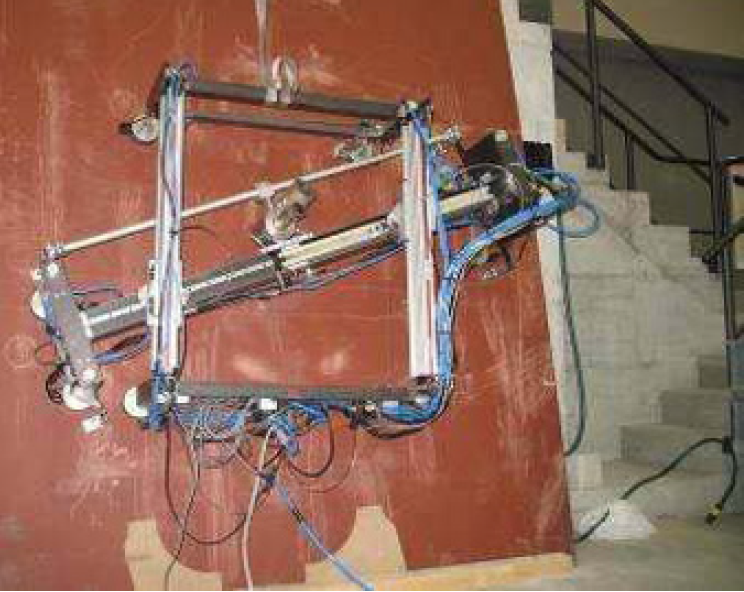
\includegraphics[width=\columnwidth]{sota/figs/climbers/grit.png}
\caption{Climbing robot for Grit Blasting}
\label{grit}
\end{figure}

\emph{The Climber} (figura~\ref{icm}), ICM Robotics, é um robô para inspeção de
turbinas eólicas, remoção de revestimento, limpeza de superfície, e aplicação de revestimento.
Possui adesão pneumática (sucção) e locomoção por esteiras. 

As características principais do robô são: base com capacidade de carga de 25
kg; base com locomoção de precisão milimétrica; manipulador modular pode ser
acoplado à base; manipulador de dimensão reduzida e baixa velocidade; e
locomoção apresenta restrição a algumas curvaturas acentuadas.

\begin{figure}[ht]
\centering
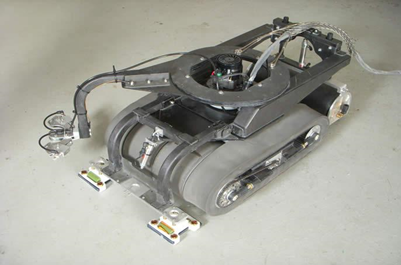
\includegraphics[width=\columnwidth]{sota/figs/climbers/icm.png}
\caption{Robô The Climber da ICM Robotics}
\label{icm}
\end{figure}

O ROMA II (figura~\ref{roma2}), Universidade Carlos II de Madrid, é um robô para
inspeção de ambientes complexos. A sua tecnologia de adesão é pneumática (sucção) e
locomove-se como uma lagarta (biomimética). Sua movimentação e planejamento de
trajetória são realizados de maneira ótima de forma a garantir estabilidade e
evitar obstáculos. 

As características principais do robô são: base com grande capacidade de carga;
base com locomoção de precisão milimétrica; não possui manipulador; locomoção em
ambientes de grande complexidade.

\begin{figure}[ht]
\centering
%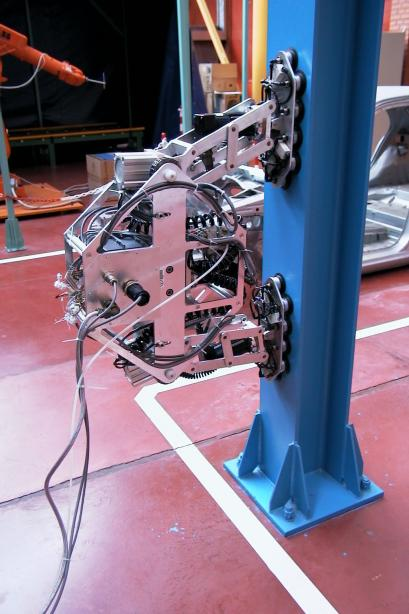
\includegraphics[width=8.4cm]{sota/figs/climbers/roma2.jpg}
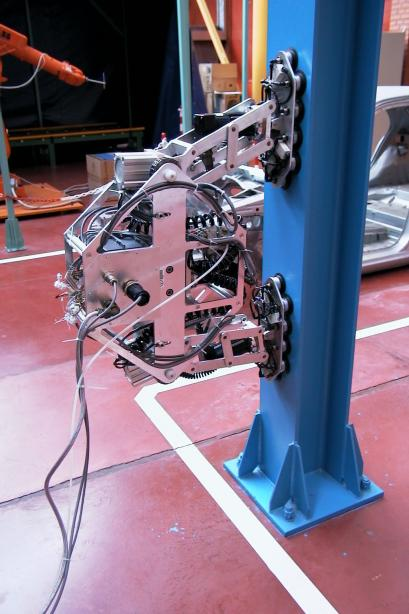
\includegraphics[width=\columnwidth]{sota/figs/climbers/roma2.jpg}
\caption{ROMA II.}
\label{roma2}
\end{figure}

CROMSCI (figura~\ref{cromsci}), Kaiserslautern University of Technology, é um
robô autônomo para inspeção de grandes paredes de concreto, como pilares de pontes, barragens. Seu
sistema de adesão é composto por sete câmaras de vácuo (sucção), com um sistema
de controle por válvulas e sensores de pressão para reagir rapidamaente a
condições adversas. Locomove-se com rodas omnidirecionais para locomoção.

As características principais do robô são: base com pouca capacidade de
carga; base com locomoção de precisão milimétrica; não possui manipulador; e
apresenta baixa velocidade.

\begin{figure}[ht]
\centering
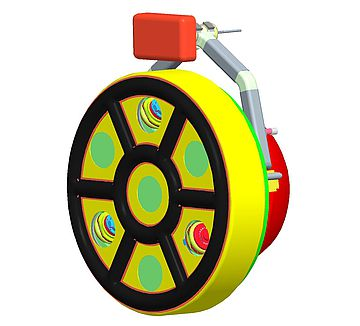
\includegraphics[width=\columnwidth]{sota/figs/climbers/cromsci.jpg}
\caption{Robô CROMSCI.}
\label{cromsci}
\end{figure}

TRIPILLAR (figura~\ref{tripillar}), École polytechnique fédérale de Lausanne, é
um robô escalador de pequeno porte (96 x 46 x 64 mm) desenvolvido para a inspeção de plantas
petroquímicas. Utiliza um sistema como pernas de lagarta magnéticas em um
formato triangular. Locomove-se por esteiras.

As características principais do robô são: base com pouca capacidade de
carga; base com locomoção de precisão milimétrica; sistema robusto a aplicações
em ambientes de alta periculosidade; sistema de controle simples; robô de
pequenas dimensões; não possui manipulador; sistema ainda não testado em estruturas geométricas complexas.


\begin{figure}[ht]
\centering
\includegraphics[width=\columnwidth]{sota/figs/climbers/tripillar.png}
\caption{Robô TRIPILLAR.}
\label{tripillar}
\end{figure}
   
Os robôs escaladores são utilizados em diversas aplicações e possuem diferentes
soluções de aderência e locomoção, como foi exposto nesta subseção. Não há,
até o momento, um robô escalador que possui todas as características
exigidas para a tarefa de HVOF em pás de turbinas, porém a adaptação de
alguns desses sistemas, como \emph{The Climber} da ICM Robotic, pode gerar
soluções completas.

As vantagens e desvantagens para solução de robôs escaladores são:

\textbf{Vantagens:}
\begin{itemize}
  \item Facilidade de instalação;
  \item Manipulador de pequenas dimensões, já que o robô se movimenta sob a pá
  da turbina;
  \item Base de pequenas dimensões;
  \item Pouco peso;
  \item Autonomia durante a operação em uma pá; 
\end{itemize}

\textbf{Desvantagens:}
\begin{itemize}
  \item Sistema de locomoção complexo com desvio de obstáculo e planejamento de
  trajetória;
  \item Desafio mecânico na construção de uma estrutura capaz de sustentar seu
  peso mais o manipulador com sistema HVOF;
  \item Robô deve ser manualmente instalado em cada pá ou um complexo sistema
  de locomoção por braços deverá ser desenvolvido;
  \item Sistema de segurança do robô deverá ser bem desenvolvido;
  \item Bateria limitada ou sistema de gerenciamento de umbilical para robôs
  móveis;
\end{itemize} 
\subsection{Robôs cabeados}
São classificados como robôs cabeados quaisquer sistemas robôticos que façam
uso de um conjunto de cabos e/ou cordas para auxiliar ou mesmo garantir seu
posicionamento adequado na sua região de trabalho. Sendo assim, robôs cabeados
podem possuir outros métodos de fixação em conjunto com seu cabeamento.

A idéia do uso de um sistema de cabos surge naturalmente quando o deslocamento
se mostra majoriamente restrito a um plano vertical e não há exigência de
grandes velocidades de deslocamento. O sistema é usado como forma de reduzir o
preso e melhorar o desempenho de um braço mecânico de mesmo alcance, ou diminuir a complexidade e
a força de aderência necessária para um escalador.

Para exemplificar essa categoria foram selecionados dois robôs. O
\textit{torboMate} é um escalador que possui adesão magnética que o
permite caminhar livremente. Pode ter dois ou um
emissor de jatos com capacidade para abastecimento em até 4000 bar. Possui 45 kg
e atinge uma velocidade de até 20 m/min \citep{torbo}.

\begin{figure}[ht]
	\centering
	\includegraphics[width=8.4cm]{sota/figs/cables/torbo}
	\caption{Robô TorboMate "Crawler", \cite{torbo}}
	\label{fig:cables:torbo}
\end{figure}

RIWEA é um robô puramente cabeado, no sentido em que ele não possui nenhum
outro tipo de forma de ajuste de posição além do sistema de cabos. É um
conceito de robô de estrutura aberta que faz uso de quatro cordas para se
deslocar verticamente \citep{jeon2012maintenance}. Seu maior diferencial reside
na capacidade de se adaptar a curvatura da pá mantendo sempre um ponto de apoio
sobre ela, sendo também menos suceptivel a vibrações \citep{riwea}.

\begin{figure}[!h]
	\centering
	\includegraphics[width=\columnwidth]{sota/figs/cables/riwea}
	\caption{Robô RIWEA, sua cinemática adaptável ao formato da pá, \cite{riwea}}
	\label{fig:cables:riwea}
\end{figure}

Em geral, podemos sumarizar as caraterísticas do robôs cabeados segundo as
seguintes vantagens e desvantagens.

\textbf{Vantagens:}
\begin{itemize}
  \item Redução da carga sobre a fixação do robô / maior capacidade de carga.
  \item Alcance do robô pelo cabeamento pode ser estendido a baixo custo.  
\end{itemize}

\textbf{Desvantagens:}
\begin{itemize}
  \item Complexidade do sistema de gestão do cabeamento.
  \item Necessidade de um ponto de apóio superior para fixação dos cabos.
\end{itemize}



\subsection{Manipulador com base esférica}
Um projeto de pesquisa e desenvolvimento foi apresentado em
\cite{motta2010prototype} com o objetivo de propor metodologia, simulação e
os passos para construção de um sistema robótico para recuperar danos materiais
em pás de turbinas hidráulicas. O sistema robótico faz
reparo utilizando a tecnologia de soldagem a arco elétrico, antes realizada
manualmente em ambientes de alta periculosidade com temperaturas que variam
entre $40^o C$ e $99^o C$, e operações que duram em torno de 10 horas. 

O robô deve atender aos seguintes requisitos:
\begin{itemize}
  \item Capacidade de operar em qualquer posição: horizontal, vertical,
  invertida;
  \item Pouco peso para portabilidade e fixação às pás;
  \item Rigidez à deflexão: carga no punho do manipulador ocorre em qualquer
  direção e extensão;
  \item Grande precisão;
  \item Disponibilidade de peças no mercado;
  \item Controle com interface de usuário;
  \item Grande área de trabalho;
  \item Facilidade de adesão às pás de turbinas hidráulicas.
\end{itemize}

A solução para o sistema robótico apresenta topologia esférica, como pode ser
visto na figura~\ref{fig:esferico} e características:

\begin{figure}[ht]
\centering
\includegraphics[width=8.4cm]{sota/figs/esferico/esferico.jpg}
\caption{Ilustração do projeto do manipulador com base esférica.}
\label{fig:esferico}
\end{figure}

\begin{itemize}
  \item Três (3) graus de liberdade no manipulador (2R1P) e dois graus de
  liberdade no punho (2R);
  \item Mapeamento de superfície 3D com laser;
  \item Eletrônica embarcada;
  \item Soldagem por arco elétrico;
  \item Fixação nas pás por dispositivos magnéticos ou de sucção;
  \item Baixo custo;
  \item Área de trabalho em forma de anel com 2.5 m e 60 cm de altura;
  \item Peso 30 kg e dimensões 30 x 25 x 100 cm;
  \item Robô com manipulador autônomo;
\end{itemize}

O sistema robótico de manipulador com base esférica apresenta solução compatível
para a aplicação de HVOF em pás de turbinas hidráulicas, já que sua aplicação
original é soldagem das pás, semelhante ao desafio deste artigo. Todas as suas
características são vantagens e aplicam-se à solução de um sistema para HVOF.
Há, porém, desafios particulares na metalização das pás e que são desvantagens
da solução:

\textbf{Desvantagens:}
\begin{itemize}
  \item A metalização deve ser realizada em toda a pá. Portanto, o sistema
  deverá ser manualmente trocado de posição, pelo menos 4 vezes (duas posições
  para a frente e duas posições para a região de trás). E deve ser trocado de pá
  em pá;
  \item O efetuador deve percorrer a pá com grande velocidade, como exige o
  processo de metalização.
\end{itemize}

\section{Projeto de robô autônomo para HVOF}\label{sec:sota/projeto}

O projeto de robôs autônomos para HVOF em pás de turbinas hidráulicas contempla
as soluções que atendem a \textbf{todos} os requisitos da aplicação. Dessa
forma, serão idealizados sistemas robóticos com a fusão das tecnologias expostas
na seção~\ref{sota} e no contexto da usina hidrelétrica de Jirau. Também serão
desenvolvidos conceitos para movimentação e adequação dos equipamentos para
HVOF, como pistola, aspirador para recolhimento abrasivo, compressor e outros
elementos da solução.

Na seção~\ref{sec::consideracoes}, os acessos ao aro câmara foram
descritos e suas restrições são fundamentais para a elaboração da solução.
Esta seção é dividida em soluções de sistemas robóticos para os dois tipos
de acessos, já que estes são o fator que mais restringe o desenvolvimento do
sistema robótico por limitar suas dimensões, funcionalidades, e exigir a
idealização conjunta de uma logística de acesso e movimentação do robô pelo aro
câmara.
 
\subsection{Acesso pela escotilha supeior}
Essa escotilha localizada no topo do aro câmara possui uma abertura de apenas
35 cm de diâmetro, o que cria um desafio quando se pensa em utiliza-la como
ponto de acesso para um robô. Por outro lado sua proximidade às pás e a área livre fora do aro
câmara criam possibilidades interessantes para seu uso.

\textbf{Vantagens}
\begin{itemize}
  \item Estabilidade da fixação do robô
  \item Ponto de referência, facilitando sistemas de localização, mapeamento, controle e calibração
  \item Pórtico rolante para posicionar o robô na escotilha
\end{itemize}

\textbf{Desvantagens}
\begin{itemize}
  \item Dificuldade de encontrar robôs de tal dimensão (35 cm diâmetro)
  \item Necessidade de retirar e inserir o robô quando rodar as pás
  \item Solução não geral, específica para UHE Jirau
\end{itemize}

A solução mais simples para este acessso é a utilização de um robô industrial
comercial. A escolha do robô está primariamente associada ao seu alcance. Por outro lado, apenas
uma pequena parcela dos robôs comerciais possuem a dimensão necessária para
atravessar a escotilha. Sendo assim, o estudo foi direcionada para o uso do
KUKA Light Weight (LBR iiwa 14 R820), robô cuja diagonal da base é inferior aos
35 cm da escotilha.

O LBR R820 pesa 30 kg, possui 7 eixos e suporta carga de 14kg,
suficiente por uma pequena margem para carregar o equipamento de
revestimento. Entretanto, são necessários estudos aprofundados para valida-lo,
como os requisitos de velocidade e precisão quando percorrendo a trajetória
para a realização do revestimento.

Tendo como objetivo posicionar o LBR R820 em uma posição onde seja capaz de
trabalhar toda a pá, um modelo de base articulada foi proposto. A base
composta de dois elos interligados por uma junta de rotação é fixada na
própria escotilha. Para que seja possível cobrir toda a pá,
a base deve ser capaz de assumir diversas angulações com respeito ao
eixo de inserção, e a junta que conecta os dois segmentos da base também precisa
ter sua posição alterada, o que pode ser realizado manualmente ou com atuador.

Introduzir o robô, composto pelo conjunto base-LBR R820, é uma tarefa cuidadosa
pois a extensão total será maior que a distância do topo do aro câmara ao
cone da turbina. Ou seja, o braço e a base precisarão ser rotacionados
durante o processo de inserção, o que acarretará no desalinhamento do centro de
massa (com relação ao eixo perpendicular à escotilha) e exigirá uma guia para
resistir ao torque gerado por esse desalinhamento.

Com o robô fixado na escotilha e a junta da base travada, são esperados torques
inferiores a 3000 Nm sobre a junta e 4000 Nm sobre a base, durante a operação de
revestimento.

%Ao se avaliar as possibilidades de realizar o revestimento sem a necessidade de
%placas de sacrifício, percebe-se que poderá ser realizado se a junta da
%base estiver paralela à pá (que para efeito de cálculo foi assumida com uma
%angulação de $45^o$ com relação ao eixo da turbina). Para esse caso a junta
% precisa realizar uma rotação à velcidade mínima de 34 rad/min. Essa velocidade possibilita a
%pistola de revestimento percorrer verticalmente a pá sem pausa. Percorrer
%horizontalmente a pá não será possível devido às restrições nas dimensções da
%base. O cálculo foi realizado por um estudo puramente geométrico, utilizando as
%informações reais de extensão da pá e área de trabalho do robô, assumindo um
%modelo simples da pá, sem curvatura.


\subsection{Acesso pela escotilha inferior}
Soluções que utilizem o acesso pela escotilha inferior, de dimensão maior,
apresentam as seguintes vantagens e desvantagens:

\textbf{Vantagens}:
\begin{itemize}
  \item Abertura maior para passagem de robôs pequenos montados ou um robô
  grande desmontado;
  \item O acesso é livre;
  \item Este acesso já é usado pelos operadores para manutenção da turbina;
\end{itemize}

\textbf{Desvantagens}
\begin{itemize}
  \item Não é suficientemente grande para entrada de robôs de grande
  porte montados;
  \item Infraestrutura de transporte e complexidade logística ao acesso por
  andaimes e talhas;
  \item Dificuldade de movimentação e posicionamento do robô no aro câmara
  devido ao piso escorregadio e inclinado. Pode haver a necessidade de montagem
  de um plano horizontal; 
\end{itemize}

O acesso pela escotilha inferior apresenta, como todos os outros
acessos, um desafio logístico e o desafio comum do processo de metalização. O
acesso à escotilha é realizado por uma abertura de 80 mm de diâmetro e 4 m acima
do solo, logo os equipamentos são transportados por uma talha operada manualmente,
instalada dentro do aro câmara, em andaimes. O solo é escorregadio e, devido à
forma cilíndrica do aro câmara, curvilíneo e inclinado.

Dessa forma, as soluções foram focadas em robôs de médio porte, peso reduzido
devido ao transporte e às necessidades de movimentação e posicionamento do robô
(trajeto escotilha à pá), e modular, quando possível.

As soluções foram divididas em subseções de acordo com a fixação:
robôs móveis que se locomovem em trilhos, robôs escaladores e manipuladores
industriais com base fixa. 
%obs.:
%Colocar o robô entre as pás para aplicar revestimento de duas pás com uma
% instalação exige que o robô seja desmontado toda vez que a turbina for girada.
%Isso é ruim, pois após primeira aplicação a área fica de risco. Esta solução
%exige 5 movimentos no robô e 6 movimentos na turbina.

%A solução em que o robô fica atrás ou à frente exige que o robô seja
%movimentado apenas 2 vezes e a turbina fará 8 movimentos (duas voltas).

%TODO revisar todos os projetos sabendo as respostas
\subsubsection{Projeto de robôs em trilhos}\label{proj_rail}
 % attach a rail to the blade and move it manually
 
 % attach a rail one the nose and ground, 1D movement and move the blade to
A utlização de um manipulador robótico sobre trilhos satisfaz todos os
requisitos para a realização de um processo de inspeção e metalização utilizando a técnica HVOF. O desenvolvimento
de um sistema compacto para o transporte através do acesso pela escotilha
inferior e sua instalação no aro câmara da turbina são possíveis, pois as
dimensões do manipulador podem ser reduzidas por meio da
mobilidade extra proporcionada pela introdução do trilho.

No contexto da aplicação proposta, foram concebidas duas possibilidades para a
fixação do sistema de trilhos. A primeira solução consiste em um sistema
semelhante ao Roboturb, apresentado na seção \ref{sec::rail}. O sistema proposto
se trata de um manipulador robótico com fixação diretamente na pá da
turbina. O trilho deverá ser flexível para ser capaz de acompanhar a curvatura
da pá e possibilitar diversas opções de posicionamento. Como o material da pá
não possui alta permeabilidade magnética (Inox 420), a solução de fixação seria
por ventosas ativas e com material específico para suportar as grandes
variações de temperatura que a pá pode alcançar (temperatura ambiente a
$100^oC$ durante a metalização).

Uma abrangente pesquisa de robôs comerciais industriais de pequeno porte apontou
que há manipuladores com carga entre 12 e 20 kg e velocidade necessários,
sendo o LBR da Kuka o que possui melhor benefício peso/alcance, 30 Kg e 820 mm,
respectivamente. %Para este manipulador, a metalização deverá ser
%realizada em, pelo menos, quatro etapas com quatro trilhos diferentes e
%customizados, e placas de sacrifício para evitar mau aplicação da metalização
%durante as trocas de sentido na movimentação do robô.

A fixação de um trilho na pá apresenta diversas complexidades, como: a
necessidade de manualmente instalar/desinstalar o sistema trilho/robô diversas
vezes em cada pá; o projeto do trilho customizado e flexível; e ventosas ativas
especiais que suportam variação de temperatura.

A alternativa para se evitar o contato com a pá consiste em um único trilho
retilíneo fixado por bases magnéticas ou solda, no solo do aro câmara. Como o
robô não possui alcance de toda a pá, há, ainda, a necessidade de posições
verticais diferentes. A pá pode ser processada em movimentos circulares ou
lineares e, em ambos os casos, o manipulador ficará responsável pela velocidade,
posição e orientação do processo. A troca de sentido de movimento deverá
ocorrer fora da pá ou devem ser utilizadas placas de sacrifício. A

Esse tipo de abordagem simplifica a movimentação do robô no
trilho, uma vez que o trilho seria totalmente reto, e possibilitaria a
metalização de um dos lados das quatro pás com uma única instalação de base.
Porém, mesmo nesta solução, a altura do trilho deverá ser ajustada três vezes para
cada lado de pá.

Em ambos os sistemas propostos, é necessária a implementação de um sistema de
localização do robô em relação à pá, tornando possível a geração de um
planejamento de trajetórias para o processo de metalização. O sistema de
localização pode ser concebido por sensores externos
ao robô (câmeras e outros), ou instalados no próprio manipulador/base.

\paragraph{Conclusão da solução por robôs em trilhos}

A solução com trilho externo se mostrou vantajosa em comparação ao robô em
trilho customizado acoplado à pá, devido à complexidade e intervenções
manuais. Há a possibilidade de utilizar um manipulador industrial, tornando o
foco do projeto em processamento de sinais, mapeamento, localização e controle,
além da construção do trilho. Porém, a montagem da estrutura e a instalação de
todo o sistema atrás da pá podem ser custosas, sendo esta ainda uma solução
considerada complexa.
\subsubsection{Projeto de robôs escaladores}\label{proj_climbers}

Nesta subseção, consideram-se soluções para HVOF de pás de turbinas robôs
escaladores com fusão das tecnologias documentadas na
seção~\ref{sota}, subseção~\ref{sota_climbers}. Será abordada uma versão
adaptada do robô \emph{The Climber}, ICM, dado sua possibilidade de
reconfiguração.

O robô \emph{The Climber}, ICM, é uma solução comercial que atende muitas das
especificações HVOF e possibilita aperfeiçoamento sem comprometer sua
estrutura. O robô possui sistema de adesão por sucção e locomoção através de
esteiras flexíveis. O sistema já foi testado em ambientes de alta
periculosidade, como turbinas eólicas, usinas hidrelétricas e outros. Podemos
dividir o projeto em quatro sistemas: locomoção, adesão, manipulador e autonomia.

O sistema desenvolvido em \cite{kim2008development} tem mecanismo de
locomoção por esteiras e adesão por sucção. O sistema é composto por polias,
correias de borracha, ventosas, válvulas para cada ventosa, motores DC para as polias,
sistemas de controle para as válvulas e para os motores. \emph{The Climber}
utiliza apenas uma câmara de vácuo, em vez de ventosas, e esteiras flexíveis que
permitem maior suavidade e continuidade ao movimento. A solução por uma única
câmara parece mais vantajosa, já que o robô consegue se locomover em curvaturas
de até 30 cm de raio.

No caso específico da aplicação HVOF, o processo é realizado com
manipulador enquanto o robô percorre a pá da turbina. A locomoção do
robô sob a pá levanta algumas questões de projeto: a
temperatura da turbina durante o procedimento exige uma solução por câmara ativa 
de material especial; e como se comporta o robô em curvaturas
acentuadas. 

Em sistemas de adesão por sucção, deve-se considerar um mecanismo
inteligente de segurança, possivelmente utilizando acelerômetros e outros
sensores, para garantir o desligamento do sistema eletrônico e o fornecimento de
gáses. A solução de um robô móvel com planejamento de trajetória aumenta a
segurança da operação e o controle ótimo do mecanismo de adesão pode limitar a força máxima de sucção.

O manipulador a ser projetado para aplicação HVOF possui as seguintes
características: é leve para não comprometer a adesão e equilíbrio do sistema
móvel; rápido e preciso conforme requer a aplicação HVOF; modular, já
que a operação será realizada in-situ, em espaço confinado;
não possui grandes dimensões, pois o robô é móvel e pode
percorrer a pá, porém deve ser suficiente para operar em pontos de
difícil acesso à base e considerar a distância mínima (230 mm) entre pistola
HVOF e pá; e é capaz de sustentar a carga e vibrações geradas pela
pistola HVOF. 

A solução de robôs escaladores exige planejamento de trajetórias tanto da base
móvel, quanto ao controle de manipuladores. A literatura sobre
manipuladores é bastante consolidada, sendo muitos dos problemas citados já
resolvidos e disponíveis no mercado, como o desenvolvido em
\cite{manzdevelopment}. Os menores manipuladores industriais que sustentam a
carga do sistema de metalização possuem em torno de 30 a 50 kg. Portanto, o
conjunto manipulador, pistola e cabos pode possuir de 50 a 80 kg de massa.

%A tecnologia que verifica a necessidade de
%revestimento, com sensores laser e ultrassom, e poderá indicar o \textbf{mapa
%ou apenas realizar um teste de sucesso/falha} \citep{escaler2006detection}.

O sistema autônomo de um robô móvel é a inteligência do robô. Ele abrange o
controle de missão, ou seja, o planejamento e execução das tarefas em modo
autônomo. A locomoção será realizada pelo controle dos motores em conjunto com o
controle do sistema ativo de adesão por sucção, o planejamento de trajetória, desvio de
obstáculos e mapeamento do ambiente, através de um conjunto de sensores, como
laser e acelerômetros. O controle do manipulador poderá ser cinemático por
servovisão ou pela estruturação do ambiente. E um sistema de suporte do veículo
ficará responsável pela segurança, bom funcionamento e gerenciamento de potência
do robô.

As características descritas acima como solução de um robô escalador impede a
troca automática entre pás. Um robô escalador com tecnologia de avanço pendurado
por braços é uma solução muito custosa em termos de controle e estrutura
mecânica. Outra solução seria um robô com locomoção por segmentos deslizantes,
como o RRX3, e adesão por sucção, porém a flexibilidade exigida para a locomoção
entre pás e a distância entre turbinas complexifica o projeto. Dessa forma, a
troca entre pás deverá ser manual.

%\textbf{Versão adaptada Roboturb}

%O Roboturb, como já descrito na subseção~\ref{sec::rail}, é um
%manipulador que se locomove em um trilho, este acoplado à pá da turbina
%por ventosas (sucção). A solução não permite a extensão
%do manipulador, já que o peso desequilibra a estrutura e não há torque para
%compensar a força exercida no efetuador durante a operação HVOF. A segunda
%solução de robôs escaladores é adicionar um trilho perpendicular e transformar
%o Roboturb em um robô móvel, com locomoção através de dois trilhos, idéia
%semelhante ao \emph{Climbing robot for Grit Blasting}, que utiliza duas
%plataformas deslizantes com ventosas.

%Os trilhos são compostos por esteiras flexíveis nas extremidades para a
%locomoção, como \emph{The Climber}, e as ventosas são ativas e distribuídas por
%todo o trilho. O manipulador só necessitaria mover em um dos trilhos para
%percorrer toda a pá, já que os trilhos também se movimentam. 

%A solução de trilhos móveis com manipulador é dependente à curvatura da pá da
%turbina e o aumento da flexibilidade do trilho para se locomover sob a pá pode
%impedir a movimentação do manipulador. Dessa forma, é considerada uma solução
%muito específica e restrita à aplicação.

\paragraph{Conclusão da solução por robôs escaladores}
Apesar de tentador devido à autonomia, a complexidade da estrutura da pá, o
ambiente, a velocidade requerida e a carga do sistema de metalização são
grandes desafios ao projeto. São estimados 50 kg de
carga para o conjunto manipulador, cabos e pistola, o que aumenta muito as
dimensões da base móvel e, consequentemente, diminui a sua área de atuação,
tornando o processo mais demorado.
\subsubsection{Projetos com manipuladores industriais fixos}\label{proj_manip}
Há diversos manipuladores robóticos industriais com as especificações
necessárias para a realização da tarefa de metalização por HVOF. As empresas
Fanuc, Motoman, ABB e KUKA fabricam manipuladores com dimensões compatíveis com o
acesso pela escotilha inferior e velocidade, precisão, e espaço de trabalho que
cumprem os requisitos para a execução do processo em todo um lado da pá, em uma
base fixa. Porém, há incompatibilidade atrás da pá e a necessidade de escolher a
posição correta do manipulador em relação à pá, a fim de maximizar a sua área de trabalho, no ambiente da
turbina, o que pode restringir os seus movimentos.
Como as pás podem ser giradas até um ângulo de $14.5^o$, são discutidas as ideias de posicionamento
do manipulador entre as pás, a fim de executar a operação em ambos os lados da
pá (um lado de cada pá), e o posicionamento fixo à frente e depois atrás à pá.

\paragraph{Posicionamento entre pás}

A figura~\ref{fig::andaime} mostra o espaço entre as pás da turbina, dentro do
aro câmara. Um robô manipulador de médio porte pode ser fixado em uma base
magnética, na posição que se encontra o operário da figura~\ref{fig::andaime}.
Essa posição é vantajosa por possibilitar a execução da tarefa em duas pás
(frente de uma e verso da outra), sem desmontar ou fazer grandes alterações no
posicionamento da base do robô, diminuindo as intervenções e tempo de tarefa.
 
\begin{figure}[h!]
\centering
\includegraphics[width=0.7\textwidth]{figs/andaime.jpg}
\caption{Espaço entre as pás da turbina.}
\label{fig::andaime}
\end{figure}

O estudo puramente geométrico demonstra que o alcance do manipulador robótico
para o processamento de ambos os lados das pás, considerando uma base fixa entre
as pás, deverá ser em torno de 5 metros. O manipulador industrial IRB5500,
desenvolvido pela ABB para pintura, possui 3 metros de alcance, porém 180 kg, o que já dificulta ou até impossibilita a
logística de movimentação e posicionamento in-situ. Não foi encontrado um robô
industrial com o alcance necessário e que tivesse as dimensões máximas da
escotilha inferior. 

A solução conceitual de posicionar um manipulador industrial entre as pás deve
avaliar, portanto, todas as configurações necessárias da base (orientações e
posições) para garantir que todo o espaço de trabalho do manipulador mais base
cubra os lados de ambas as pás. O número de configurações e o projeto
mecânico da base são necessários para a viabilização da solução,
uma vez que será possível avaliar as intervenções e complexidades. Bases
autônomas diminuem o número de intervenções e aumentam a precisção do sistema,
porém aumentam a complexidade, o custo devido ao número de sensores e atuadores,
e o peso do sistema, prejudicando a logística.

\paragraph{Posicionamento à frente e atrás da pá}

Posicionar de maneira fixa um manipulador com base magnética à frente e atrás da
pá para a metalização é uma solução natural, já que é semelhante à utilizada pela
empresa Rijeza atualmente. Um estudo puramente geométrico, utilizando as
dimensões da pá, mostra que o manipulador deve possuir alcance de 1.7 m e ser
posicionado a uma altura de 1.1 m em relação ao solo. Estudos de espaço de
trabalho, manipulabilidade e colisões devem ser realizados para confirmar o
estudo geométrico.

O posicionamento do sistema à frente ou atrás da pá exige intervenções para
rotação da turbina e para o deslocamento do sistema. Em relação a um
sistema com base autônoma entre as pás, o processo parece mais custoso em
intervenções manuais e mais demorado, porém bem mais simples em termos de
robótica.

\paragraph{Conclusão da solução com manipuladores industriais}
A utilização de manipuladores industriais é a mais simples, em termos de
sistemas robóticos, dentre todas as soluções para o acesso pela escotilha
inferior.
Não há projeto mecânico do manipulador, já que este será adquirido em um dos fabricantes citados. As dificuldades mecânicas do projeto serão em relação à logística de posicionamento
e movimentação do robô dentro do aro câmara, e no desenvolvimento de uma base,
que pode ser autônoma. Além disso, o projeto fica responsável pelo controle do
manipulador, processamento de dados que envolvem o HVOF, planejamento de
trajetórias e interface de usuário.

Os desafios consistem na construção de uma base rígida e a locomoção dos
equipamentos pelo aro câmara. Este projeto conceitual será uma das frentes para
o estudo de viabilidade.
 
%% TODO Elael: Nosso projeto cabeado
\subsubsection{Robô Bipartido}

Esse conceito é uma cadeia de dois manipuladores conectados por um ponto de
apoio capaz de fixar-se à pá. O apoio serve como forma reduzir o torque
necessário nas juntas ao reduzir a alcance necessário para cada manipulador
individualmente.

Para facilitar futuras referências nesse texto, o braço robótico que se
apoia sobre o chão será chamado de primário, manipulador que parte dele de
secundário e o ponto de apoio entre eles, capaz de fixa-se à pá, será chamado de
fixador.

A pistola de metalização presa ao manipulador secundário deve ter
alcance sobre toda a pá da turbina. Para isso existe uma gama de pontos
necessários onde o fixador deve ser posicionado. Com esse intuito o
manipulador primário da cadeia precisa ser projetado para ter uma região de
trabalho com um alcance total sobre esses pontos. Para tal, informações precisas
sobre o formato das pás são necessárias.

Para viabilizar a solução, é necessário verificar quais são as soluções
possíveis para gerar a aderencia do fixador sobre à pá. As tecnologias mais
difundidas são por força magnética e por diferença de pressão (ventosa).
As maiores preocupações com o relação a adesão são a capacidade de carga do
método e a resistência do \textit{coating}. As soluções por magnetismo e
por ventosa afetam de maneira diferente as camadas do material ao qual se
aderem. Enquanto o magnetismo atrai ativamente o material ao qual prentende
aderir, a ventosa apenas reduz a pressão do ar na região onde ela se fixa. Ambas
as soluções possuem versões ativas e passivas, assim como uma gama de opções com
relação à capacidade de suportar carga. Logo, para essas soluções, a carga
necessária a ser suportada, o magnetismo do material, a resistência à baixa
pressão do \textit{coating} e os efeitos da atração magnética, também, sobre o
\textit{coating} são perguntas que devem ser respondidas.

O braço secundário deve ser projetado para atingir os requerimentos de
posicionamento e velocidade da pistola de metalização, porém a região sob o
fixador, certamente, não estará disponivel para receber o revestimento. Assim, a
possibilidade, ou os requisitos necessários, de mover o fixador para uma região
da pá recém metalizada deve ser vista analisada antes do robô bipartido ser
considerado uma possibilidade.

\subsection{Robô Pendurado} 

\subsection{Qualificação do processo HVOF}

O método de revestimento HVOF foi descrito na Seção~\ref{sec::desc_hvof}. É um
processo de aplicação de revestimento onde partículas metálicas (com ou sem carbonetos) de
aproximadamente 5 a 60 microns são projetadas através de uma chama supersônica
até a superfície que se deseja metalizar, a fim de aumentar a vida útil dessa
superfície contra os desgastes de corrosão, abrasão, erosão e cavitação.
Utilizando propano como combustível, obtêm-se uma aplicação com as seguintes
características: temperatura de chama 2700° C; velocidade da chama de até 2100
m/s; velocidade de partícula 700 m/s; pressão de combustão 80 PSI.

Com este processo é possível aplicar ligas metálicas com carbonetos produzindo
revestimentos densos, com baixo volume de óxidos, alta adesão ao substrato e
dureza de até 1400 HV. O processo de HVOF possui os seguintes elementos:

\begin{itemize}
\item Uma pistola de aplicação, onde é realizada a combustão e projeção do
revestimento contra a superfície das pás. Esta deverá estar montada no robô;
\item \textit{Flowmeter} para controle das pressões e vazões dos gases, onde é
regulada a pressão e vazão do O2, Propano e ar comprimido. Deve ser montado
fora do circuito hidráulico, porém o mais próximo possível da escotilha;
\item Alimentador de pó para a pistola, onde é regulado a vazão de pó que é
alimentado para a pistola de aplicação. Deve ser montado fora do circuito
hidráulico, porém o mais próximo possível da escotilha;
\item Cilindros de proprano (estudar necessidade de vaporizador). Combustível 
do processo;
\item Cilindros de O2: comburente do processo;
\item Cilindros de N2: gás de arraste do pó para a pistola;
\item Compressor e secador de ar para a refrigeração da pistola, próximo ao
\textit{Flowmeter};
\item \textit{Chiller} água gelada para refrigeração da pistola. Deve estar
próxima ao \textit{Flowmeter};
\item Estufa para armazenamento da matéria prima;
\item Transformadores de energia 110V;
\item Bomba para compensar queda de pressão da água;
\item Base com rodízio para movimentação dos equipamentos até a escotilha;
\item Exaustor para controle da umidade, temperatura e concentração de gases;
\end{itemize}
 
O projeto de HVOF \textit{in situ} para UHE Jirau busca solucionar os problemas
descritos na seção~\ref{sec::consideracoes}. Dessa forma, as subseções seguintes
abrangem a acessibilidade e movimentação dos equipamentos ao ambiente da
turbina; os principais tipos de revestimentos que resistam a esses desgastes; e
a forma de preparo da superfície por jateamento.

\subsubsection{Movimentação e acessibilidade}
A Fig.~\ref{fig:proj_hvof_1} detalha o circuito hidráulico da turbina de
Jirau. O caminho às escotilhas são superior e inferior são distintos. A
escotilha superior pode ser alcançada por uma plataforma de acesso às unidades
geradoras (1), e uma descida por meio de ponte rolante (2). O caminho à
escotilha inferior é complexo: há uma escada (3) de
aproximadamente 23 metros até a área de descarga (4); do ponto (4) até o
corredor (5) que leva à escotilha são mais 4.77 metros pelo corredor (6), o qual
possui 2.3 metros de altura; por fim, é preciso subir uma escada (7) com
aproximadamente 6 metros de altura por 1,7 de largura.

\begin{figure}
	\centering
	\includegraphics[width=1\columnwidth]{sota/figs/projeto/proj_hvof_1.png}
    \caption{Desenho esquema com acesos ao circuito hidráulico.}
    \label{fig:proj_hvof_1}
\end{figure}

A Fig.~\ref{fig:proj_hvof_2} mostra o acesso pela escotilha superior
do aro câmara, e a posição onde os equipamentos podem ficar alocados. A
Fig.~\ref{fig:proj_hvof_3} apresenta o conceito de posicionamento dos
equipamentos levando em consideração o acesso pela escotilha inferior.
Os conceitos de movimentação dos equipamentos são gaiolas para alocação através
de olhais para movimentação vertical e espaço para encaixe de paleteira para
movimentação horizontal dos acesórios para metalização, representados na
Fig.~\ref{fig:proj_hvof_4}.

\begin{figure}
	\centering
	\includegraphics[width=1\columnwidth]{sota/figs/projeto/proj_hvof_2.png}
    \caption{Acesso pela escotilha superior do aro câmara.}
    \label{fig:proj_hvof_2}
\end{figure}

\begin{figure}
	\centering
	\includegraphics[width=1\columnwidth]{sota/figs/projeto/proj_hvof_3.png}
    \caption{Acesso pela escotilha inferior.}
    \label{fig:proj_hvof_3}
\end{figure}

\begin{figure}
	\centering
	\includegraphics[width=1\columnwidth]{sota/figs/projeto/proj_hvof_4.png}
    \caption{Sistemas de movimentação do Jato e eqipamentos acesórios à pistola de Coating.}
    \label{fig:proj_hvof_4}
\end{figure}

\subsubsection{Jateamento abrasivo}

Na Seção~\ref{sec:jat}, o jateamento abrasivo foi introduzido como requisito
para a preparação da superfície a ser revestida. Foram investigados duas
alternativas para posicionamento e a forma de execução do equipamento
para preparação superficial com óxido de alumínio. Em ambos os casos, a 

\begin{enumerate}
  \item Máquina de jato com reservatório deverá permanecer fora do circuito
  hidráulico, porém o mais próximo possível da escotilha. A pistola de
  jateamento com recirculação do abrasivo; Compressor de ar com secador:
  secador de ar deve estar próximo a maquina de jato; Sistema de filtragem de
  ar mandado ao operador para abastecer ar filtrado para respiração
  do operador, fora do circuito hidráulico.
  \item Máquina de jato com reservatório do abrasivo deverá permanecer fora do
  circuito hidráulico, porém o mais próximo possível da escotilha. Pistola sem
  sistema de recirculação de abrasivo; Aspirador para recolhimento do abrasivo;
  Compressor de ar com secador ar próximo à maquina de jato; Sistema de
  filtragem de ar mandado ao operador para abastecer ar filtrado
  para respiração, fora do circuito hidráulico.
\end{enumerate}

O jato com sistema recirculante é uma alternativa interessante, porém pode
possuir menor produtividade.

\subsubsection{Tipos de revestimentos}

Para se determinar a solução ideal de revestimento para as pás Kaplan,
primeiramente foram mapeados os principais tipos de desgastes que sofrem os
equipamentos de hidrogeração. Esse mapeamento foi realizado através de estudo
teórico em materiais de fabricantes de equipamentos hidrelétricos, artigos em
revistas científicas e inspeção própria nas unidades geradoras de Jirau. Na
Fig.~\ref{fig:proj_hvof_5}, está apesentada uma das principais regiões
desgastadas pelas pás e os tipos de danos por abrasão, cavitação, erosão e corrosão.

\begin{figure}
	\centering
	\includegraphics[width=1\columnwidth]{sota/figs/projeto/proj_hvof_5.png}
    \caption{Mapeamento do desgaste das pás da UHE Jirau através de inspeção em campo.}
    \label{fig:proj_hvof_5}
\end{figure}

A partir desse mapeamento prévio foram selecionados três tipos de materias para
o revestimento das pás, Tabela~\ref{tab::materiais_HVOF}.

\begin{table}[]
\centering
\caption{Materiais base para HVOF}
\label{tab::materiais_HVOF}
\begin{tabular}{ccc}
\hline
Sistema                                                                  & Material                                                                                                                                                         & Principal aplicação do revestimento                                                         \\ \hline
\multicolumn{1}{|c|}{WCNiCr}                                             & \multicolumn{1}{c|}{\begin{tabular}[c]{@{}c@{}}Material base em AISI 410 e revestimento de \\ Carboneto de Tungstênio em matriz\\ de Niquel Cromo\end{tabular}}  & \multicolumn{1}{c|}{\begin{tabular}[c]{@{}c@{}}Desgaste\\ Erosivo e Cavitação\end{tabular}} \\ \hline
\multicolumn{1}{|c|}{WCCoCr}                                             & \multicolumn{1}{c|}{\begin{tabular}[c]{@{}c@{}}Material base em AISI 410 e revestimento de \\ Carboneto de Tungstênio em matriz\\ de Cobalto-Cromo\end{tabular}} & \multicolumn{1}{c|}{\begin{tabular}[c]{@{}c@{}}Desgaste\\ Abrasivo e Erosão\end{tabular}}   \\ \hline
\multicolumn{1}{|c|}{\begin{tabular}[c]{@{}c@{}}AISI\\ 410\end{tabular}} & \multicolumn{1}{c|}{\begin{tabular}[c]{@{}c@{}}Material base \\ em aço inoxidável AISI 410\end{tabular}}                                                         & \multicolumn{1}{c|}{---}                                                                    \\ \hline
\end{tabular}
\end{table}

Para qualificar os materiais e as modificações nos equipamentos foram
realizados ensaios baseando-se em procedimentos normatizados. Abaixo é feita a
listagem dos testes realizados bem como a norma a qual aquele teste se
relaciona. Os testes estão classificados em duas categorias: testes para
qualificação do processo, e testes para a seleção do revestimento.

Os testes para qualificação do processo são:

\begin{enumerate}
  \item \textbf{Ensaio de adesão:} Norma Relacionada: ASTM C633; Equipamento
  utilizado: Máquina de ensaios universal; Corpos de prova: 3 corpos de prova
  cilíndricos de 1 polegada de diâmetro para cada conjunto de testes;
  \item \textbf{Microdureza:} Norma Relacionada: ASTM E384; Equipamento
  utilizado: Microdurômetro Vickers com carga de 0.1 à 1 kgf Corpos de prova:
  Retangulares com 25,4 mm x 10 mm x 5 mm. 1 por teste;
  \item \textbf{Medição de Porosidade e Óxidos:} Norma Relacionada: ASTM E2109
  Equipamento utilizado: Microscópio óptico com lentes objetivas de 50 até 1000
 x de aumento. Corpos de prova: Retangulares, os mesmos utilizados para o ensaio
 de microdureza.
  \item \textbf{Rugosidade:} Norma Relacionada: ISO 4287-1997; Equipamento
  utilizado: rugosimetro portátil para medição dos parâmetros Ra, Rz.
  Corpos de prova: serão utilizados os mesmo corpos de prova para o ensaio de
  microdureza.
\end{enumerate}

Os testes para a seleção do revestimento são:
\begin{enumerate}
  \item \textbf{Ensaio de Erosão:} Norma Relacionada: ASTM G76;
  Equipamento utilizado: equipamento de erosão por partículas sólidas;
  Corpos de prova: retangulares com 25,4x15 mm por 5 mm de espessura. Ou 30 mm
   de diâmetro. 3 por teste.
  \item \textbf{Ensaio de Abrasão:} Norma Relacionada: ASTM G65;
  Equipamento utilizado: abrasômetro do tipo roda de borracha;
  Corpos de prova: retangulares de 25,4 x 76 x 5 mm mínimo;
   \item \textbf{Ensaio de Cavitação:} Norma Relacionada: ASTM G32;
    Equipamento utilizado: equipamento de vibração ultrasônico.
   \item \textbf{Ensaio de Imersão – Corrosão:} Norma Relacionada: -//-
   Equipamento utilizado: cuba de imersão e potenciostato;
  Corpos de prova: retangulares com 25,4x20 mm por 5 mm de espessura. 3 por
  teste.
   \item \textbf{Adesão por dobramento:} Norma Relacionada: ASTM B571;
Equipamento utilizado: Dispositiva para dobramento em máquina de ensaio universal
Corpos de prova: 50 x 75 x 3 mm;
\end{enumerate}

\textbf{Demais equipamentos utilizados para controle do processo de
Jateamento e Metalização:}
Termo-higrômetro para medição do ponto de orvalho e controle da umidade relativa do ar;
Pirômetro para controle da temperatura da peça/corpo de prova;
Rugosimetro para medição da rugosidade da superfície jateada e metalizada;
Medidor de camada indutivo para controle da espessura de camada;

\textbf{Accura-Spray para controle da temperatura e velocidade da chama
hipersônica:} Este ensaio é de grande importância para a qualificação dos
procedimentos de HVOF na medida que ele monitora os parâmetros de saída da chama de aspersão
como a temperatura e a velocidade média das partículas. A
Fig.~\ref{fig:proj_hvof_6} mostra o cabeçote do equipamento accura spray
montado próximo à pistola de aspersão para monitoramento de chama.

\begin{figure}
	\centering
	\includegraphics[width=1\columnwidth]{sota/figs/projeto/proj_hvof_6.png}
    \caption{Cabeçote do accura spray para monitoramento da chama de aspersão
    témica.}
    \label{fig:proj_hvof_6}
\end{figure}
%\subsection{Acesso pela jusante}
Como última opção de acesso ao rotor, existe a possibilidade de utilização do
tubo de sucção ou descarga como meio de entrada à turbina. Com o fluxo de água
parado, é possível utilizar o Rio como meio de lançamento do sistema. A
complexidade da operação para utilizar esse acesso é maior, entretanto existem
vantagens que podem tornar essa solução viável e mais atrativa.

\textbf{Vantagens}
\begin{itemize}
  \item Virtualmente nenhuma restrição de tamanho
  \item Flexibilidade de soluções
  \item Facilidade de utilização de um manipulador industrial padrão
  \item Possibilidade de implementação em outras usinas
\end{itemize}

\textbf{Desvantagens}
\begin{itemize}
  \item Complexidade de lançamento e recuperação
  \item Custo
  \item Possibilidade de correnteza
  \item Complexidade logística de transporte entre a entrada do tubo de sucção e
  o aro câmara
  \item Complexidade de prototipação
\end{itemize}

As soluções foram divididas em etapas necessárias para a operação, ou
seja, lançamento e recuperação do sistema, logística de transporte e o robô de
metalização propriamente dito.

Para esse acesso, o maior obstáculo presente é o desenvolvimento de um sistema
de lançamento e recuperação do robô, a partir do rio, até o interior da turbina.
Essa operação deverá ser realizada com a turbina alagada e, em seguida,
pode-se dar início ao processo de drenagem da
mesma.
É importante que o sistema de lançamento seja robusto e garanta o perfeito posicionamento do robô dentro da turbina, assim
como, a sua recuperação, uma vez que erros nesse processo podem significar a
perda completa do sistema.

Primeiramente, a solução deve ser a prova d'água com classificação para pelo
menos 50m de profundidade.
Sendo assim, um vaso de pressão para o transporte do robô até o interior da turbina deve ser
desenvolvido, não havendo necessidade do maniupulador responsável pela
metalização ser a prova d'água. O \textit{container} de transporte
submarino deve ser menor que o tamanho do vão do stoplog, visto que o acesso
mais próximo ao tubo de descarga, pelo rio, se dá por esse vão.
Por outro lado, suas dimensões devem ter um tamanho mínimo que possibilite o
encapsulamento do robô e todo o material de suporte necessário. Há aindaa
necessidade de uma escotilha de acesso de tamanho suficiente para que todo o
sistema seja retirado do interior do \textit{container} submarino.

Para o sistema de lançamento, foi deslumbrada uma estrutura de transporte que
utilizará o pórtico rolante e o trilho guia dos stoplogs. Após a submersão da
estrutura, um mecanismo de lançamento, inspirado em um paletizador, é
responsável pelo posicionamento do \textit{container}, sempre no mesmo ponto em
relação ao tubo de descarga. Com o vaso de pressão posicionado, a turbina deve
ser, então, drenada. Em seguida, o robô pode ser retirado de seu
envólucro e a operação de metalização pode ter seu início. Uma etapa crítica da
operação é a recuperação do sistema, na qual a turbina deve ser novamente
alagada e os os stoplogs retirados. A estrutura de transporte deve, então,
recuperar o \textit{container} transportador na mesma posição em que o sistema
foi lançado. O sucesso dessa operação tem como \textbf{hipótese que a velocidade
de drenagem e a correnteza gerada por essa operação não são suficientes para
retirar o container (mais pesado que a água) de sua posição inicial}. 

A movimentação do robô do ponto de lançamento até o aro câmara deverá ser
realizada a partir da utilização de cordas, roldanas e talhas. Caso necessário,
pode ser desenvolvido um sistema de locomoção com trilhos e/ou rodas atuadas
para o posicionamento automático do robô e, até mesmo, um plano elevado para
transporte.

O robô de metalização pode ter diversos fomatos, mas devido a possilidade de se
utilizar um manipulador industrial padrão, o projeto inicial consiste em uma
base de apoio e um manipulador com alcance para o processamento de uma face da
pá posicionado de frente para pá, ou um manipulador posicionado entre duas pás com
alcance para processar as duas as faces das pás voltadas para ele.













\subsection{Solução conceitual}
Como conclusão das propostas, a solução conceito é a utilização de um
manipulador industrial sobre uma base. A característica do manipulador e da base
varia de acordo com o ponto de acesso: no caso
da escotilha superior, a solução é um manipulador industrial de pequeno porte e
base customizada operada eletronicamente; no caso da escotilha inferior,
manipulador industrial de porte médio e base magnética; no último caso de acesso
pela jusante, será escolhido um manipulador industrial de grande porte com base
fixa magnética.
\section{Estudo de bases para manipuladores industriais}

\subsection{Modelagem 3D das soluções conceituais}
Os estudos das possíveis soluções exigiu uma visualização mais detalhada do
volume livre no interior da turbina. Para isso, foi recriado o ambiente da
turbina em CAD 3D no SolidWorks, a partir dos desenhos 2D de seção da turbina.
O modelo tridimensional do aro câmara permite o estudo e o dimensionamento geométrico de
alcance do manipulador para cada solução. Não foram necessários
detalhamentos de todos os componentes, podendo ser apenas considerados, e
representados com maior precisão, os perfis externos do túnel à montante, o
estator, o rotor e uma pequena região à jusante, além dos acessos
por escotilha superior e inferior.
A figura~\ref{fig::ambiente3d} apresenta o ambiente da turbina em CAD e os
possíveis acessos para realização das intervenções.

\begin{figure}[h!]
\centering
	\includegraphics[width=\columnwidth]{sota/figs/estudo/solid/ambiente_3d} 
	\caption{Ambiente 3D da Turbina, em SolidWorks}
	\label{fig::ambiente3d}
\end{figure}

A solução pela escotilha superior, devido ao espaço reduzido de entrada, não
permite a utilização de manipuladores de grande porte, sendo escolhido o KUKA
LBR 820. Este manipulador não possui alcance para realizar a operação em toda a
pá, exigindo uma base customizada que permita o
posicionamento do manipulador para realização das operações por etapas. Para
isso, foi estudada uma estrutura de base que permitisse diferentes
posicionamentos para o manipulador no interior do aro câmara, de forma que este
pudesse cobrir toda a superfície da pá. A base consiste em 3 braços
telescópicos que permitem a extensão do sistema para prover o alcance
necessário ao manipulador e o recolhimento para uma configuração incial que
permita a entrada do manipulador no aro câmara com segurança, sem o risco de
choques ou interferências indesejadas. Além disso, uma junta rotativa oferece mais um grau
de liberdade para o sistema, facilitando o acesso do manipulador à toda ar
superfície da pá. 

Os atuadores da base são acionados eletricamente e possuem sensores de
posicionamento. Atuadores de esferas recirculantes foram escolhidos devido à
baixa folga e precisão elevada. A estrutura da base é composta por cilindros de
diâmetro maximizado e pequena espessura, o que oferece um momento de inércia
polar elevado e baixo peso, fornecendo grande rigidez à flexão e minimizando
erros de posicionamento e vibração excessiva. A figura~\ref{fig::base_recolhida} e a figura~\ref{fig::base_extendida} apresentam
o conceito da base do manipulador em duas configurações: recolhida (configuração
de entrada) e estendida (configuração de operação).

\begin{figure}[h!]
\centering
	\includegraphics[width=0.7\columnwidth]{sota/figs/estudo/solid/Base_Recolhida.PNG} 
	\caption{Detalhes em corte da base na configuração inicial recolhida}
	\label{fig::base_recolhida}
\end{figure}

\begin{figure}[h!]
\centering
	\includegraphics[width=0.6\columnwidth]{sota/figs/estudo/solid/Base_Extendida.PNG} 
	\caption{Base na configuração totalmente extendida}
	\label{fig::base_extendida}
\end{figure}

Os componentes principais da base estão representados nas
figuras~\ref{fig::base_recolhida} e~\ref{fig::base_extendida}, são: 1) atuador
linear por sem-fim coroa; 2) base fixa; 3) braço prismático \#1; 4) braço
prismático \#2; 5) atuadores lineares; 6) junta rotativa; 7) braço prismático
\#3.

A figura~\ref{fig::base_ambiente3d_recolhida} demonstra a base com o
manipulador KUKA LBR 820 e as dimensões extremas, em milímetros, estimadas para o
interior e para fora da turbina, na configuração inicial de entrada no aro
câmara pela escotilha superior.
A figura~\ref{fig::base_ambiente3d_extendida} apresenta a base com o manipulador
em uma configuração qualquer de operação, demonstrando o ganho de alcance e
generalidade de posicionamento fornecidos pela base.

\begin{figure}[H]
\centering
	\includegraphics[width=0.6\columnwidth]{sota/figs/estudo/solid/Base_Ambiente3d_Recolhida.png} 
	\caption{Base na configuração inicial no ambiente da turbina}
	\label{fig::base_ambiente3d_recolhida}
\end{figure}

\begin{figure}[H]
\centering
	\includegraphics[width=0.6\columnwidth]{sota/figs/estudo/solid/Base_Ambiente3d_Operacao.PNG} 
	\caption{Base em uma geral configuração de operação}
	\label{fig::base_ambiente3d_extendida}
\end{figure}



%TODO: Estevão Comentar e acrescentar a nova




 
\subsubsection{Dimensionamento da base}

Para manipuladores com longo alcance, as forças e torques envolvidos requerem
uma estrutura de fixação do robô de forma que o sistema como um todo não se
movimente e, no caso extremo, tombe. Normalmente, os manipuladores robóticos são
fixados no chão e as características da superfície e tamanho dos parafusos
necessários são estipulados pelo fornecedor a partir dos valores máximos de
torque e força que o manipulador pode exercer em seu ponto de apoio.
Considerando um manipulador centrado em uma base circular apoiada no chão, dois
fatores influenciam capacidade de estabilização da estrutura: o raio da base e o seu peso.

O raio da base $r_{b}$ é limitado pelo ambiente da turbina e para cada escolha
de posicionamento existem restrições específicas. 
Para a realização dos cálculos de dimensionamento foi considerado,
primeiramente, o manipulador posicionado em frente a pá, como ilustrado na
figura \ref{fig::robot_front}.

\begin{figure}[H]
\centering
	\includegraphics[width=0.7\columnwidth]{sota/figs/openrave/robot_front_openrave.jpg}
	\caption{Exemplo de posicionamento de um manipulador robótico em frente à pá.}
	\label{fig::robot_front}
\end{figure}

 %TODO figura robo na frente da turbina
Nessa posição é possivel processar uma face por
vez, a uma altura de 1000mm do chão, desde que o manipulador tenha um alcance
mínimo de 1800mm, como especificado na seção \ref{sec::estudo_geom}. Para essa
configuração, a tamanho máximo no sentido perpendicular ao fluxo d'água que
a base pode assumir é de aproximadamente 1600mm. Existe ainda a curvatura do aro
câmara e a estrutura deve ser projetada de forma a seguir os
contornos impostos pelo ambiente.
A figura \ref{fig::base_aro_frente} 
representa um esboço da vista frontal do aro câmara e a largura máxima que a
base pode assumir. A análise da dimensão máxima da base no sentido paralelo ao
fluxo d'água pode ser realizada com o auxílio do desenho técnico fornecido pela
ESBR, ilustrado na figura \ref{fig::turbine_side}.

\begin{figure}[H]
\centering
	\includegraphics[width=0.7\columnwidth]{sota/figs/base/base_aro_frente.jpg}
	\caption{Visão frontal do aro câmara e raio máximo da base.}
	\label{fig::base_aro_frente}
\end{figure}

O limite superior do raio da base nessa
região é determinado pela região de transição do aro câmara para o tubo de
descarga, onde há uma mudança na inclinação do plano de apoio. A região,
considerada horizontal, que pode acomodar a base do manipulador tem um
comprimento de aproximadamente 1400mm no sentido do fluxo do rio.
Entrentanto, esse limite pode ser contornado construindo-se um plano de apoio
horizontal ou projetando-se a base de forma que ela acompanhe essa
inclinação.É necessário, então, considerar o dimensionamento da base no
cálculo do alcance mínimo do manipulador,que agora se encontra deslocado em
relação à superfície da pá. Sendo assim, alcance mínimo se relaciona com o tamanho do raio da base de 
acordo com $$a_{min}=\sqrt{r_b^2+1800^2}.$$

\begin{figure}[H]
\centering
	\includegraphics[width=0.7\columnwidth]{sota/figs/base/turbine_side}
	\caption{Visão lateral do aro câmara e raio máximo da base nessa direção.}
	\label{fig::turbine_side}
\end{figure}

O cálculo das dimensões da base com o robô posicionado dentro do aro câmara e
entre as pás, como ilustrado na figura \ref{fig::robot_between}, depende do
ângulo de ataque das pás.

\begin{figure}[H]
\centering
	\includegraphics[width=0.7\columnwidth]{sota/figs/openrave/robot_between_openrave.jpg}
	\caption{Exemplo de posicionamento de um manipulador robótico entre as pás.}
	\label{fig::robot_between}
\end{figure}
A distância entre as pás pode ser calculada por meio do cálculo do ângulo diédrico entre elas. A amplitude do movimento de rotação $alpha$ 
das pás é de $14,5^o$ para cada lado a partir da posição zero, entretanto \textbf{essa posição não pôde ser
informada no momento da viagem de reconhecimento e ainda não foi
disponibilizada}. Para critério de cálculos foi utilizado um ângulo de
$45^o$ como a posição de maior abertura das pás e o zero foi considerado como
a reta perpendicular ao fluxo de água. O ângulo diédrico $\theta$ entre as pás
depende do ângulo de ataque das pás e obedece a relação $\cos{\theta} =
\sin^2{\alpha}.$

O a distância entre as pás, considerada como o arco de circunferência no aro
câmara descrito pelo ângulo diédrico calculado, pode ser obtido a partir da
relação $arc=R\alpha$.
Considerando o raio do aro do câmara comoo R=3850mm, o raio máximo da base pode
ser calculado como $$r_{b_e} = (R - h_{b_e})\tan{\theta/2}$$ e com $h_{b_e}$
sendo a altura da base.

O peso mínimo que a base do robô deve possuir está diretamente relacionada com o
tamanho de seu raio. A firgura \ref{fig::tilt_robot} faz uma representação
simplificada da forma que o torque de capotamento máximo atua no robô e em sua
base. Na situação limite, considerando um torque com sentido horário, a força
normal entre a base e a superfície de apoio, $N_2$, teria módulo igual a zero.
No pior caso, podemos considerar que a força vertical exercida pelo robô em sua
base é composta apenas pelo seu peso $W$ e, para que a base não se mova, o
somatório das forças e torques devem ser iguais a zero.

A análise do somatório das forças nos fornece a relação $N_1=W$  e o somatório
dos torques se reduz a $M_k-Wr_b=0$. Sendo assim, a relação entre o raio da base, seu 
peso e o torque máximo de capotamento exercido pelo robô é
da forma 

$$M_k=Wr_b.$$

%TODO refazer figura
\begin{figure}[H]
\centering
	\includegraphics[width=0.6\columnwidth]{sota/figs/base/tilt}
	\caption{Forças e torques máximos entre o robô e sua base.}
	\label{fig::tilt_robot}
\end{figure}

%TODO comparativo entre raio e peso

Uma vez que a superfície do aro câmara e a região adjacente no tubo de sucção
são \textbf{ferromagnéticas}, é possível a utilização de bases magnéticas para
uma compensação do peso e raio necessários para a estabilização do robô. Os
dispositivos magnéticos se dispõem de duas em duas principais catergorias para
essa aplicação:
dispositivos eletretromagnéticos e de imãs permanentes. O primeiro caso tem como
principal vantagem a possibilidade de acionamento remoto, entretanto para situações de
falha em que haja perda de fornecimento de energia, a força de atração também é
perdida. O segundo caso consiste em imãs permanentes arrumados de maneira que
seja possível organizar o seu fluxo magnético e, assim, controlar por meio de
uma alavanca a presença ou ausência de força magnética. A figura
\ref{fig::base::imas} ilustra os dois tipos de bases magnéticas citados.

\begin{figure}[H]
\begin{subfigure}[b]{0.5\columnwidth}
  \centering
  \includegraphics[width=.7\columnwidth]{sota/figs/base/mangnetpipe}
  \caption{Tipo imã permanente}
  \label{fig:sfig1}
\end{subfigure}%
\begin{subfigure}[b]{0.4\columnwidth}
  \centering
  \includegraphics[width=.7\columnwidth]{sota/figs/base/eletromagnet}
  \caption{Tipo eletroimã}
  \label{fig:sfig2}
\end{subfigure}
\caption{Tipos de bases magnéticas comerciais.}
\label{fig::base::imas}
\end{figure}

Comercialmente, foram encontrados bases magnéticas com capacidade de até 3000N.
Um dos requerimentos para a utilização de bases magnéticas, sejam
eletromagnéticas e de imãs permanentes, é a limpeza da superfície de contato
para um acoplamento efeiciente. Essa restrição força a presença humana para a
limpeza e, sobretudo, a verificação de uma correta fixação. Sendo assim, as
bases magnéticas de imã permanente se mostram mais coerentes para a aplicação,
pois não possuem ponto de falha para o caso de perda de energia do sistema e
possuem uma maior capacidade de carga. A curvatura do ambiente não é um
limitante, sendo possível até a confecção de uma máscara para a base de maneira
que a superfície de apoio se conforme perfeitamente com a superfície de fixação.

%\section{Conclusão e trabalhos futuros}\label{sec:conclusions}

Este documento teve como objetivo: fazer uma análise das restrições do processo
de revestimento por aspersão térmica; caracterizar o ambiente de trabalho onde o
processo será realizado; fazer um estudo detalhado do estado da arte que
visaram solucionar um problema semelhante ou possuíam tecnologias que
poderiam ser utilizadas como solução; apresentar soluções conceituais; e
fazer um estudo de viabilidade técnica para as soluções. 

O estudo de viabilidade de uma solução para revestimento \textit{in situ} se
mostrou promissor e foram apontadas algumas possíveis soluções considerando cada
acesso ao aro câmara da turbina. Todas as soluções esbarram em alguns desafios
logísticos e técnicos que serão abordados detalhadamente até o fim do projeto
EMMA. Os projetos de bases mecânicas para as diversas soluções serão abordados,
assim como suas instalações, manuseio e posicionamento. Além disso, toda a parte
de localização, calibração e mapeamento realizado pelo robô, seu controle e
interface de usuário ainda serão desenvolvidos.


% ---------------------------------------------------------------------------
% \includepdf[pages=1-,
% addtotoc={1,section,1,Introdução,rq11[,1,section,1,Descrição do Problema,
% rq1_2[,2,subsection,2,Descrição do
% processo
% HVOF,rq1_21[,3,subsection,2,Descrição dos
% requisitos de operação de HVOF,rq1_22[,3,subsubsection,3,Jateamento da
% superfície da pá,
% rq1_221[,3,subsubsection,3,Reparo de danos
% existentes,rq1_222[,3,paragraph,4,Reparo
% com materiais não fundidos à
% superfície,rq1_2221[,3,paragraph,4,Reparo
% por solda,rq1_2222[,3,paragraph,4,Reparo por
% solda e placa
% sólida,rq1_2223[,4,subsection,2,Contextualização
% do
% ambiente,rq1_23[,4,subsubsection,3,Hélice
% e pás,rq1_231[,4,subsubsection,3,Aro Câmara e regiões
% adjacentes,rq1_232[,5,subsubsection,3,Escotilhas
% de acesso,rq1_233[,5,subsubsection,3,Tubo de
% sucção,rq1_234[,5,subsubsection,3,Infraestrutura
% disponível,rq1_235[,6,subsection,2,Descrição das
% tarefas do robô,rq1_24[,6,section,1,Estado da
% arte,rq1_3[,6,subsection,2,Robôs sobre
% trilhos,rq1_31[,7,subsection,2,Robôs
% escaladores,rq1_32[,9,subsection,2,Robôs
% cabeados,rq1_33[,10,subsection,2,Manipulador com
% base esférica,rq1_34[,11,section,1,Projeto de
% robô autônomo para
% HVOF,rq1_4[,11,subsection,2,Acesso pela
% escotilha
% superior,rq1_41[,11,subsection,2,Acesso pela
% escotilha
% inferior,rq1_42[,12,subsubsection,3,Projeto
% de robôs em trilhos,
% rq1_421[,12,subsubsection,3,Projeto de
% robôs
% escaladores,rq1_422[,13,subsubsection,3,Projetos
% com manipuladores industriais
% fixos,rq1_423[,14,subsection,2,Solução
% conceitual,rq1_43[,14,section,1,Estudo
% de bases para manipuladores
% industriais,rq1_5[,14,subsection,2,Modelagem
% 3D das soluções
% conceituais,rq1_51[,15,subsubsection,3,Dimensionamento
% da
% base,rq1_511[,17,section,1,Conclusão
% e trabalhos
% futuros,rq1_6[,18,section,1,Referências,rq1_7]]]]]]]]]]]]]]]]]]]]]]]]]]]]]]]}]{pdfs/sota}
% % ---------------------------------------------------------------------------

\chapter{Estudo de viabilidade técnica}\label{cap::detail}

\section{Introdução}\label{sec::introducao}
%TODO Renan: Introdução
%TODO Situar o Leitor do que foi concluido no SOTA.

No capítulo \ref{cap::sota}, foi apresentada a importância da manutenção regular
das turbinas em uma usina hidrelétrica, já que, em sua operação ideal e de máxima eficiência,
sua potência tem aumento de quase 46\% após manutenção. Aumento significativo,
principalmente para países dependentes desta forma de energia, como o Brasil e
Noruega.

A eficiência de uma turbina hidrelétrica depende de inúmeras variáveis, como
volume de água, queda d'água, o tipo da turbina, o distribuidor e outras. O
projeto EMMA tem foco na manutenção do perfil hidráulico das pás dos rotores de
turbinas hidrelétricas, por este se degradar com maior rapidez, exigindo
manutenções recorrentes. 

A fim de proteger a pá contra abrasão e cavitação é realizado processo de
revestimento por asperção térmica, ou, especificamente, a metalização (HVOF).
Atualmente, este processo pode levar cerca de dois meses por turbina,
já que exige que a turbina seja desmontada, as pás serem processadas em
outro ambiente, a turbina seja remontada e recalibrada.

Apesar de o projeto visar uma solução genérica para turbinas bulbo, as
instalações são diferentes em cada usina. Desta forma, o ambiente de testes
deste projeto é a Usina Hidrelétrica Jirau, localizada no Rio Madeira. O Rio
Madeira carrega muitos sedimentos provocando maior abrasão nas pás, se comparado
com outros usinas, além disso, a queda d'água de 2 a 20 metros intensifica o
fenômeno de cavitação. As principais características das instalações da turbina
em análise estão descritas no capítulo \ref{cap::sota}, mas vale ressaltar a
particularidade dos dois acessos principais ao aro câmara, relevantes para a busca de uma
solução: acesso superior (35.7 cm de diâmetro) e acesso inferior (80 cm de
diâmetro).

O projeto EMMA busca uma solução para o processo de metalização \textit{in
situ}, isto é, revestimento das pás no ambiente da turbina, diminuindo o tempo
de manutenção e, consequentemente, de máquina parada.  A solução conceitual
desenvolvida no capítulo \ref{cap::sota} é a utilização de um manipulador
industrial sobre uma base. As características do manipulador e da base variam de acordo com o
acesso: no caso da escotilha superior, a solução é um manipulador industrial de
pequeno porte e base customizada operada eletronicamente; no caso da escotilha
inferior, a solução é um manipulador industrial de porte médio e base tipo
trilho com acopladores magnéticos.

A análise das instalações da Usina Hidrelétrica de Santo Antônio, em Porto
Velho, vizinha à Jirau, mostrou que as turbinas não possuem um acesso superior.
A fim de tentar construir uma solução mais geral, o presente documento visa dar
continuidade ao projeto, detalhando o estudo de viabilidade técnica para a
solução da escotilha inferior.


\section{Estudo de viabilidade técnica detalhada}\label{sec::viatec} 
% Author: Renan

O estudo de viabilidade técnica detalhada é realizado para cada acesso à turbina
(superior e inferior), como no capítulo  \ref{cap::sota}. O estudo passa pelas
seguintes etapas: 1) pesquisa de mercado; 2) geometria plana e/ou espacial; 3)
espaço de trabalho e cinemática do manipulador; 4) detalhamento de
bases mecânicas; 5) dinâmica do manipulador; 6) sensores para calibração; 7)
planejamento de trajetórias; e 8) técnicas de calibração.
Neste documento, serão abordadas as etapas: 1, 2, 3, 4, 5 e 6.

A pesquisa de mercado é uma busca abrangente de soluções comerciais dentro do
escopo da solução conceitual desenvolvida no capítulo \ref{cap::sota}. A
pesquisa envolve manipuladores comerciais que preencham os requisitos do processo de HVOF e
estejam de acordo com as restrições impostas pelo ambiente e o acesso. Desssa
forma, diversos fabricantes de manipuladores, Motoman, Kuka, ABB, Fanuc,
Adept e Kinova, foram avaliados e suas principais características como carga,
peso, dimensões, velocidade, temperatura e umidade de operação, são analisadas.
A pesquisa de mercado tem como objetivo retornar o objeto para os outros
estudos, ou seja, o manipulador a ser utilizado na solução.

O estudo puramente geométrico, apesar de ser diferente para cada acesso, é
genericamente uma abordagem simplificada e analítica do problema e desconsidera
alguns fatores do ambiente. O estudo geométrico tem como objetivo retornar um caso
aproximado da situação real e estimar as possíveis soluções da posição do
manipulador em relação à pá, de forma que toda ela seja revestida.

O espaço de trabalho e cinemática do manipulador é uma abordagem
detalhada e de simulação. Ela considera: o meio estruturado, em um ambiente de
simulação; o manipulador com suas dimensões e limites de juntas reais;
possibilidade de colisões; real espaço de trabalho do manipulador; modelos de
bases para o manipulador; e possiveis sensores. Para a simulação é utilizada a
plataforma Openrave, uma arquitetura de planejamento para robôs autônomos,
sendo possivelmente integrada para controle em tempo real e monitoramento.
Ela provê funcionalidades para operações de cinemática direta e inversa, e
simulações físicas, e apresenta ferramentas e interfaces para planejamento de
manipuladores e um protocolo que interpreta scripts na linguagem MatLab, Octave
e Python \citep{diankov2008openrave}.

Na seção de estudo da dinâmica de manipuladores robóticos, serão realizadas
análises numéricas e analíticas, em um ambiente de simulação, de cinemática
diferencial e torques das juntas de manipuladores, utilizando as características
do processo de revestimento. O estudo tem por objetivo tornar a simulação mais
realista, analisar a execução do processo para algumas distâncias da pá
e verificar a manipulabilidade do robô.

A base mecânica é definida como a estrutura de suporte e transporte do robô.
Esta deve permitir ao manipulador alcançar os posicionamentos necessários, 
definidos nos estudos cinemáticos e dinâmicos. Para que estes
posicionamentos sejam alcançados, a base mecânica oferece graus de
liberdade ao sistema base e robô, adequados para levar a base do robô aos pontos
ótimos para o revestimento de uma região da pá. Como principais diretrizes para
o projeto da base mecânica, são considerados: a resistência aos esforços dinâmicos do
manipulador; baixas vibrações; modularidade; e facilidade de transporte,
montagem e ajuste. O estudo dos conceitos analisados para a base mecânica serão
demonstrados em detalhe na seção~\ref{sec::base_mec}.

As características e desafios logísticos da escotilha inferior já foram
previamente apresentados no capítulo \ref{cap::sota}, sendo aqui apontadas, na
tabela~\ref{tab::bighatch}, apenas as suas principais caracterísiticas para o
desenvolvimento de uma solução detalhada.

\begin{center}
\begin{tabular}{  c | c  }
  \hline
  \textbf{Informação} & \textbf{Dado} \\ \hline
  Dimensões do acesso & 800 mm de diâmetro  \\ \hline
  Distância do acesso à pá & 4000 mm  \\ \hline
  Distância do solo & 5000 mm \\ \hline
  Peso máximo manipulável & 150 Kg \\
  \hline
\end{tabular}
\captionof{table}{Dados principais da escotilha inferior}
%\caption{Dados principais do processo de metalização HVOF}
\label{tab::bighatch}
\end{center}

\subsection{Pesquisa de mercado}
% Author: Renan
A pesquisa de mercado está detalhadamente explicada na
tabela~\ref{ape::bighatch}, no apêndice. Os seguintes robôs satisfazem os
requerimentos e restrições principais, de acordo com as tabelas~\ref{tab::bighatch} e ~\ref{tab::hvof}, e os requisitos abordados
em \ref{sec::desc_contex}: Viper s1300 (Adept), ARC Mate 100iC/12 (Fanuc),
M-10iA/12S (Fanuc), LBR iiwa 14 R820 (Kuka), KR 10 R1100 sixx WP (Kuka), MH6F-10
(Motoman), SIA10F (Motoman), MH12 (Motoman), SIA20D (Motoman). Destes, os
manipuladores LBR iiwa 14 R820 (Kuka) e Viper s1300 (Adept) deverão passar por adaptações para
operar em temperaturas até $40^o$C e umidade relativa no ar de $91\%$; e os
manipuladores KR 10 R1100 sixx WP (Kuka), MH6F-10
(Motoman) e SIA10F (Motoman) têm carga máxima de 10 Kg, que é o limite para o
processo. Dessa forma, os manipuladores comerciais prontos para o uso e que
trabalha com folga em carga são: ARC Mate 100iC/12 (Fanuc), M-10iA/12S (Fanuc),
MH12 (Motoman) e SIA20D (Motoman).

Apesar de o manipulador LBR iiwa 14 R820 (Kuka) necessitar de adaptações, seu
peso (29 Kg) representa grande vantagem perante os outros manipuladores, logo
não deve ser descartado em futuros estudos. O mesmo se pode dizer do KR 10 R1100
sixx WP (Kuka), que possui 56 Kg, mas estará operando perto de sua carga limite
(10 Kg).

Os objetos de estudo são, portanto: KR 10 R1100
sixx WP (Kuka), MH12 (Motoman), LBR iiwa 14 R820 (Kuka), ARC Mate 100iC/12
(Fanuc) e SIA20D (Motoman).


 
\subsection{Estudo puramente geométrico}
% Author: Renan
A abordagem puramente geométrica é uma análise do espaço de trabalho do
manipulador na pá. Utiliza os manipuladores da pesquisa de mercado como
objetos deste estudo e leva em consideração as dimensões da
pistola, o ângulo máximo e mínimo para o revestimento ($90^o \pm 60^o$), e a
distância mínima de 230 mm entre a pistola e a pá. É um estudo simplificado por não considerar as possíveis colisões com o ambiente, assumir
que a pá está contida em um plano (projeção, objeto 2D) e considerar o espaço
de trabalho do manipulador simétrico. A abordagem geométrica foi desenvolvida
com o auxílio do software Geogebra.

Primeiramente, o espaço de trabalho do manipulador é aproximado
como uma esfera, delimitada pelo espaço de
trabalho real do manipulador. A pá é projetada em planos, como mostra a
figura~\ref{fig::paplanos}, e, conforme o manipulador se aproxima da pá, o plano
direito corta a esfera (espaço de trabalho do manipulador), FIGURA. A interseção
entre o plano e a esfera é um círculo de raio $\overline{CB^i}$, que pode ser
calculado e estimado como a área revestida da pá. A distância ótima entre o
manipulador e a pá é calculada no limite em que o ângulo
$\overline{OB^iC}=30^o$. Finalmente, podem ser calculadas quantas posições
distintas o manipulador deve assumir para que toda a pá seja revestida, a partir
do modelo planar da pá e da turbina, figura~\ref{fig::pa2D}.

Essa abordagem é específica para cada manipulador da pesquisa de mercado.

\begin{figure}[h!]
	\centering	
	\includegraphics[width=0.6\columnwidth]{detail/figs/bighatch/PaPlanos.PNG}
	\caption{Ilustração das projeções da pá em planos.}
	\label{fig::paplanos}
\end{figure}

\begin{figure}[h!]
	\centering	
	\includegraphics[width=0.6\columnwidth]{detail/figs/bighatch/pa2D.png}
	\caption{Ilustração do modelo 2D da pá.}
	\label{fig::pa2D}
\end{figure}

\paragraph{KR 10 R1100 sixx WP (Kuka)}
A figura~\ref{fig::kukageom} ilustra a interseção do espaço de trabalho
simplificado do manipulador Kuka KR10 e a projeção da pá. No
caso do Kuka KR 10 R1100, o raio da esfera é aproximado a $\overline{OB^i} = $
alcance do manipulador + comprimento da pistola + 230 mm. 

Para este manipulador, obtemos área revestida de $1.41^2\pi m^2$ e distância
ótima manipulador-pá de $0.82 m$. Dessa forma, são necessárias, pelo menos,
quatro posições distintas do manipulador a fim de toda a pá ser revestida. A
figura~\ref{fig::kukacircles} ilustra os pontos que o manipulador deve assumir
para revestir toda a pá. 

\begin{figure}[h!]
	\centering	
	\includegraphics[width=0.6\columnwidth]{detail/figs/bighatch/kukageom.jpg}
	\caption{Ilustração da interseção do espaço de trabalho simplificado do
	manipulador Kuka KR10 e a projeção da pá.}
	\label{fig::kukageom}
\end{figure}

\begin{figure}[h!]	
	\centering
	\includegraphics[width=0.6\columnwidth]{detail/figs/bighatch/kukacircles.png}
	\caption{Posições do manipulador Kuka KR10 para o processo de
	revestimento ser realizado em toda a pá.}
	\label{fig::kukacircles}
\end{figure}

\paragraph{MH12 (Motoman)}
A figura~\ref{fig::mh12geom} ilustra a interseção do espaço de trabalho
simplificado do manipulador MH12 e a projeção da pá. No
caso do MH12, o raio da esfera é aproximado a $\overline{OB^i} = $
alcance do manipulador + comprimento da pistola + 230 mm. 

Para este manipulador, obtemos área revestida de $1.54^2\pi m^2$ e distância
ótima manipulador-pá de $0.89 m$. Dessa forma, são necessárias, pelo menos,
duas posições distintas do manipulador a fim de toda a pá ser revestida. A
figura~\ref{fig::mh12circles} ilustra os pontos que o manipulador deve assumir
para revestir toda a pá.		

\begin{figure}[h!]	
	\centering
	\includegraphics[width=0.6\columnwidth]{detail/figs/bighatch/mh12geom.jpg}
	\caption{Ilustração da interseção do espaço de trabalho simplificado do
	manipulador Motoman MH12 e a projeção da pá.}
	\label{fig::mh12geom}
\end{figure}

\begin{figure}[h!]	
	\centering
	\includegraphics[width=0.6\columnwidth]{detail/figs/bighatch/mh12circles.png}
	\caption{Posições do manipulador MH12 para o processo de
	revestimento ser realizado em toda a pá.}
	\label{fig::mh12circles}
\end{figure}
\subsection{Espaço de trabalho e cinemática do
manipulador}\label{sec::cinematica} 
% Author: Renan

Como já mencionado, o ambiente de simulação
foi desenvolvido utilizando a arquitetura de planejamento Openrave. Para cada manipulador selecionado após a
pesquisa de mercado, serão analisados os reais espaços de trabalho, e o processo de
revestimento da pá em um ambiente simulado que representa as principais
caracterísiticas do ambiente real.

Para gerar o espaço de trabalho, o Openrave utiliza um método de força bruta,
onde são executadas iterações sob iterações de todas as juntas, por seus ângulos
limites e com o passo de ângulo dependendo da resolução do manipulador. O grau
de manipulabilidade do robô é representado por um gradiente de cores, cujo grau
varia do azul claro (menor manipulabilidade) ao vermelho escuro (maior manipulabilidade).
Entende-se por manipulabilidade a capacidade que o robô possui de manipular
objetos em direções específicas, isto é, para uma posição específica é
possível alcançar variadas orientações. Em todas as simulações, a pistola foi
representada como um cilindro de comprimento 300 mm e raio 50 mm, e o efetuador está no extremo do cilindro.

A superfície da pá é amostrada, formando uma grade de tamanho fixo. A técnica
\textit{axis-aligned bounding box (AABB)} é utilizada para obter os
pontos e suas respectivas normais, na superfície da pá. Nesta técnica, a
superfície alvo é inscrita em um bloco, que é uniformemente amostrado. É, então,
realizada uma verificação de colisão entre os pontos amostrados no bloco e a
superfície alvo e, caso haja interseção, o ponto é armazenado junto com sua
normal à superfície. Dessa forma, podemos amostrar a pá e deslocar estes pontos
230 mm em relação à sua normal com a superfície, garantindo a requerimento do
revestimento. A representação dos pontos amostrados e deslocados em relação às
normais da pá podem estão nas figuras~\ref{fig::amostrapa1} e ~\ref{fig::amostrapa2}. 

Utilizando as informações dos pontos amostrados e o espaço de trabalho do
manipulador, foram gerados scripts para calcular a
melhor distância do manipulador em relação a pá, de forma que o maior número de
pontos revestidos com angulação de $90^o$ fossem cobertos.
Essa distância é calculada em relação à normal da pá. Com esse dado, é possível estimar quantas posições da base do
manipulador serão necessários para o revestimento de toda a pá.

\begin{figure}[h!]	
	\includegraphics[width=\columnwidth]{detail/figs/bighatch/amostrapa1.png}
	\caption{Pontos amostrados da pá - vista lateral}
	\label{fig::amostrapa1}
\end{figure}

\begin{figure}[h!]	
	\includegraphics[width=\columnwidth]{detail/figs/bighatch/amostrapa2.png}
	\caption{Pontos amostrados da pá - vista frontal}
	\label{fig::amostrapa2}
\end{figure}

As tabelas~\ref{tab::robocarac} e ~\ref{tab::robocarac} abaixo resume as
caracterísitcas de cada robô e o estudo cinemático realizado, respectivamente:

\begin{center}
\begin{tabular}{  c | c | c | c  }
  \hline
  \textbf{Robô} & \textbf{Payload (Kg)} & \textbf{Massa (Kg)} & \textbf{Alcance
  (mm)} \\ \hline 
  KR10 & 10 & 56 & 1100 \\ \hline
  MH12 & 20 & 130 & 2551  \\ \hline
  LBR 14 & 14 & 30 & 820 \\ \hline
  SIA20D & 20 & 120 &  910 \\
  \hline
\end{tabular}
\captionof{table}{Caracterísitcas principais dos robôs.}
\label{tab::robocarac}
\end{center}

\begin{center}
\begin{tabular}{  c | c | c }
  \hline
  \textbf{Robô} & \textbf{Pontos revestidos (\%)} & \textbf{Posições de base} \\ \hline 
  KR10 & 24.33 & 13\\ \hline 
  MH12 & 53.3 & 4   \\ \hline
  LBR 14 $\uparrow$ & 17.2 & 13 \\ \hline
  LBR 14 $\rightarrow$ & 17.37 & 13 \\ \hline
  SIA20D $\uparrow$ & 23.14 & 9 \\ \hline
  SIA20D $\rightarrow$ & 24.76 & 9 \\ 
  \hline
\end{tabular}
\captionof{table}{Resumo do estudo
cinemático.}
\label{tab::robocin}
\end{center}

\paragraph{KR 10 R1100 sixx WP (Kuka)}
A figura~\ref{fig::kr10cin1} e figura~\ref{fig::kr10cin2} mostram as vistas
lateral e superior do espaço de trabalho do manipulador, respectivamente. Em
vermelho, estão representados os pontos a serem revestidos e em preto os pontos
que o manipulador foi capaz de revestir.

O script que calcula a melhor posição da base em relaçao à pá retornou a posição
870 mm, sendo que 3825 pontos foram revestidos, representando 24.33\% de toda a
pá. Estima-se que serão necessários, pelo menos, 13 posições para o recobrimento
de toda a pá, figura~\ref{fig::kr10bestpos}.



\begin{figure}[h!]	
	\includegraphics[width=\columnwidth]{detail/figs/bighatch/kr10_front.png}
	\caption{Espaço de trabalho do manipulador Kuka KR10 - vista lateral}
	\label{fig::kr10cin1}
\end{figure}

\begin{figure}[h!]	
	\includegraphics[width=\columnwidth]{detail/figs/bighatch/kr10_top.png}
	\caption{Espaço de trabalho do manipulador Kuka KR10 - vista superior}
	\label{fig::kr10cin2}
\end{figure}

\begin{figure}[h!]	
	\includegraphics[width=\columnwidth]{detail/figs/bighatch/kr10_bestpos.png}
	\caption{Melhor posição para o revestimento - robô KR10 da Kuka.}
	\label{fig::kr10bestpos}
\end{figure}


\paragraph{MH12 (Motoman)}
A figura~\ref{fig::mh12cin1} e figura~\ref{fig::mh12cin2} mostram as vistas
lateral e superior do espaço de trabalho do manipulador, respectivamente.

O script que calcula a melhor posição da base em relaçao à pá retornou a posição
950 mm, sendo que 8379 pontos foram revestidos, representando 53.30\% de toda a
pá. Estima-se que serão necessários, pelo menos, 4 posições para o recobrimento
de toda a pá, figura~\ref{fig::mh12bestpos}.

\begin{figure}[h!]	
	\includegraphics[width=\columnwidth]{detail/figs/bighatch/mh12_front.png}
	\caption{Espaço de trabalho do manipulador MH12 - vista lateral}
	\label{fig::mh12cin1}
\end{figure}

\begin{figure}[h!]	
	\includegraphics[width=\columnwidth]{detail/figs/bighatch/mh12_top.png}
	\caption{Espaço de trabalho do manipulador MH12 - vista superior}
	\label{fig::mh12cin2}
\end{figure}

\begin{figure}[h!]	
	\includegraphics[width=\columnwidth]{detail/figs/bighatch/mh12_bestpos.png}
	\caption{Melhor posição para o revestimento - robô MH12 da Motoman.}
	\label{fig::mh12bestpos}
\end{figure}


\paragraph{LBR iiwa 14 R820 (Kuka)}
O manipulador LBR iiwa 14 R820 possui 7 graus de liberdade e, devido a sua
grande flexibilidade e facilidade de montagem, foram estudadas duas
configurações para a base.

O script que calcula a melhor posição da base na posição vertical em relaçao à
pá retornou a posição 1.06, sendo que 2648 pontos foram revestidos,
representando 17.20\% de toda a pá. Estima-se que serão necessários, pelo menos,
13 posições para o recobrimento de toda a pá, figura~\ref{fig::lbrbestposv}.

\begin{figure}[h!]	
	\includegraphics[width=\columnwidth]{detail/figs/bighatch/lbr_bestposv.png}
	\caption{Melhor posição para o revestimento - robô LBR da Kuka com base na
	posição vertical.}
	\label{fig::lbrbestposv}
\end{figure}

O script que calcula a melhor posição da base na posição vertical em relaçao à
pá retornou a posição 1400 mm, sendo que 2730 pontos foram revestidos,
representando 17.37\% de toda a pá. Estima-se que serão necessários, pelo menos,
13 posições para o recobrimento de toda a pá, figura~\ref{fig::lbrbestposh}.

\begin{figure}[h!]	
	\includegraphics[width=\columnwidth]{detail/figs/bighatch/lbr_bestposh.png}
	\caption{Melhor posição para o revestimento - robô LBR da Kuka com base na
	posição horizontal.}
	\label{fig::lbrbestposh}
\end{figure}

\paragraph{SIA20D (Motoman)}
O manipulador SIA20D também possui 7 graus de liberdade e, devido a sua
grande flexibilidade e facilidade de montagem, foram estudadas duas
configurações para a base.

O script que calcula a melhor posição da base na posição vertical em relaçao à
pá retornou a posição 1100 mm, sendo que 3638 pontos foram revestidos,
representando 23.14\% de toda a pá. Estima-se que serão necessários, pelo menos,
9 posições para o recobrimento de toda a pá, figura~\ref{fig::sia20dbestposv}.

\begin{figure}[h!]	
	\includegraphics[width=\columnwidth]{detail/figs/bighatch/sia20d_bestposv.png}
	\caption{Melhor posição para o revestimento - robô SIA20D da Motoman com base
	na posição vertical.}
	\label{fig::sia20dbestposv}
\end{figure}

O script que calcula a melhor posição da base na posição horizontal em relaçao à
pá retornou a posição 1510 mm, sendo que 3892 pontos foram revestidos,
representando 24.76\% de toda a pá. Estima-se que serão necessários, pelo menos,
9 posições para o recobrimento de toda a pá, figura~\ref{fig::sia20dbestposh}.

\begin{figure}[h!]	
	\includegraphics[width=\columnwidth]{detail/figs/bighatch/sia20d_bestposh.png}
	\caption{Melhor posição para o revestimento - robô SIA20D da Motoman com base
	na posição horizontal.}
	\label{fig::sia20dbestposh}
\end{figure}

\paragraph{Tolerância no ângulo de revestimento}
As análises de revestimento dos manipuladores exigiram que a pistola
estivesse com as mesmas direções e sentidos opostos às normais dos
pontos a serem revestidos, isto é, a orientação da pistola é sempre
perpendicular ao plano da pá. Entretanto, pode-se assumir uma tolerância de
$90^o \pm 60^o$ entre a pistola e o plano perpendicular, que foi considerada
na análise puramente geométrica. Como o manipulador MH12 (Motoman) possui
recobrimento de quase todo o alcance vertical da pá (revestimento de cima a
baixo), mostra-se interressante a análise de tolerância neste manipulador, de
forma que haja simplificação das possíveis soluções de bases.

Primeiramente, são armazenados os pontos que o robô não foi capaz de
revestir (pontos em vermelho, nas figuras de espaço de trabalho dos
manipuladores) e suas respectivas normais aos planos tangentes à superfície da
pá. Os pontos são deslocados 230 mm na mesma direção e sentido oposto às suas
respectivas normais, de forma que pertençam à superfície da pá,
ponto $D$ é deslocado até ponto $C$ na figura~\ref{fig::tolerancia1}. Para cada
ponto não revestido, são gerados dois vetores unitários $\overrightarrow{v}$ e
$\overrightarrow{w}$ ortogonais entre si e ao vetor normal $\overrightarrow{N}$,
no plano tangente à superfície da pá, conforme
ilustrado na figura~\ref{fig::tolerancia2}. O vetor $\overrightarrow{N}$ é
girado pelo ângulo de tolerância de revestimento $\theta$ (entre $0^o$ e $60^o$)
em relação ao vetor $\overrightarrow{w}$, gerando o vetor
$\overrightarrow{P_1}$, figura~\ref{fig::tolerancia3}.

\begin{figure}[h!]	
	\includegraphics[width=\columnwidth]{detail/figs/bighatch/tolerancia1.png}
	\caption{Ponto D não revestido, deslocado 230 mm da superfície da pá.}
	\label{fig::tolerancia1}
\end{figure}

\begin{figure}[h!]	
	\includegraphics[width=\columnwidth]{detail/figs/bighatch/tolerancia2.png}
	\caption{Vetores v e w ortogonais ao vetor normal N.}
	\label{fig::tolerancia2}
\end{figure}

Finalmente, o vetor $\overrightarrow{P_1}$ pode ser girado em relação a
$\overrightarrow{N}$ e todos os vetores que pertencem à tolerância de
revestimento $\theta$ saem do ponto $C$ até um ponto do círculo $h$, como o
vetor exemplo $\overrightarrow{P_2}$, na figura~\ref{fig::tolerancia4}. Observe
que este círculo deve ser discretizado, e cada ponto pertencente ao círculo e sua
respectiva normal (vetor de origem $C$ ao ponto do círculo) devem ser
reavaliados, isto é, verifica-se se o robô alcança o ponto pertencente a $h$ com
pistola de revestivemto apontada a sua respectiva normal.
Se algum ponto do círculo puder ser revestido, o ponto $D$ pode ser considerado
como revestido. No exemplo da figura~\ref{fig::tolerancia4}, o círculo $h$ foi
discretizado em dois pontos $G$ e $H$, e suas normais são $\overrightarrow{P_1}$
e $\overrightarrow{P_2}$, respectivamente. 

\begin{figure}[h!]	
	\includegraphics[width=\columnwidth]{detail/figs/bighatch/tolerancia3.png}
	\caption{Vetor N girado pelo ângulo de tolerância de revestimento.}
	\label{fig::tolerancia3}
\end{figure}

\begin{figure}[h!]	
	\includegraphics[width=\columnwidth]{detail/figs/bighatch/tolerancia4.png}
	\caption{Circulo $h$ representa todos os pontos equivalentes ao ponto $D$ com
	ângulo de tolerância de revestimento $\theta$.}
	\label{fig::tolerancia4}
\end{figure}

Foram realizadas análises de tolerância para dois robôs: MH12, que apresentou o
maior número de pontos revestido na pá, e LBR R820, que é a única solução viável
de manipulador industrial para o acesso superior. Os ângulos de tolerância foram
variados em $10^o$ e $30^o$. 

\subsection{Dinâmica do manipulador}\label{sec::dinamica}
% Author: Renan

A dinâmica de um manipulador robótico é a análise de velocidades, acelerações e
torques das juntas. Para esta análise, assume-se que o efetuador, pistola de
revestimento, possui velocidade 40m/min constante em todos os pontos amostrados
da pá. Como velocidades e acelerações exigem a computação de derivadas, é
realizada uma melhor discretização da pá da turbina, na qual o passo de
amostragem é menor e um filtro garante espaçamento uniforme dos pontos de 10 mm.
Para um lado da pá, são amostrados, portanto, 130 mil pontos.

Para cada ponto amostrado da pá, faz-se a análise cinemática e são armazenados
os pontos que são possíveis de serem revestidos, como na
seção~\ref{sec::cinematica}, isto é, são armazenados os pontos que possuem
solução de cinemática inversa. Posteriormente, para cada ponto revestido, é
criado um conjunto contendo seus 8 pontos vizinhos através de um algoritmo k-d
tree, como na figura~\ref{fig::pontosdin}, onde $p_r$ é o ponto de referência a
ser analisado dinamicamente e os pontos ${p_1,p_2,q_1,q_2,r_1,r_2,s_1,s_2}$ são auxiliares
para o estudo. 

\begin{figure}[h!]	
	\includegraphics[width=\columnwidth]{detail/figs/dinamica/pontosdinamica.png}
	\caption{Pontos exemplo amostrados da pá.}
	\label{fig::pontosdin}
\end{figure}

%As soluções de cinemática inversa (ângulos das juntas do robô)
%$\Theta_r
%=
%{\theta_{p_r},\theta_{p_1},\theta_{p_2},\theta_{q_1},\theta_{q_2},\theta_{r_1},\theta_{r_2},\theta_{s_1},\theta_{s_2}}$
As velocidades angulares das juntas são calculadas a partir da cinemática
diferencial. Para isso, usa-se o cálculo da matriz jacobiana ($J$), que é a
diferenciação (derivadas parciais) da matriz de cinemática direta em função das
variáveis de junta \citep{sciavicco2000differential}. A velocidade linear do
efetuador ($\dot{X}$) e o jacobiano são conhecidos em cada ponto de referência, logo
podem-se calcular as velocidades das juntas do manipulador entre o ponto de
referência e cada ponto auxiliar: $\dot{X} = J\dot{q}\Rightarrow
J^+\dot{X}=\dot{q}$, onde $J^+$ é a pseudo inversa Moore-Penrose de $J$.

As velocidades angulares são $\Omega_r
=
\{\omega_{p_r,p_1},\omega_{p_r,p_2},\omega_{p_r,q_1},\omega_{p_r,q_2},\omega_{p_r,r_1},\omega_{p_r,r_2},\omega_{p_r,s_1},\omega_{p_r,s_2}\}$,
onde $\omega$, $\omega\in\Omega_r$, é um vetor $n \times 1$, e $n$ é o número de
juntas do robô. As velocidades dos ângulos das juntas é uma informação importate para a
verificação da viabilidade das trajetórias do robô. Para o caso do robô
MH12, onde $\omega_{\textbf{max}}=\{220, 200, 220, 410, 410, 610\}^o/s$, por
exemplo, caso não haja $\omega\in\Omega_r$, tal que
$\omega\leq\omega_{\textbf{max}}$, não é possível realizar o revestimento do
ponto de referência $p_r$. Se $\exists \omega\in\Omega_r$ tal que
$\omega\leq\omega_{\textbf{max}}$, o ponto de referência é viável pela
cinemática inversa e pela cinemática diferencial, mas pode ser inviável ainda
pela análise dinâmica, que considera as acelerações, massas e forças do
conjunto.

As equações dinâmicas de um manipulador são também abordados em
\cite{sciavicco2000differential} e possuem duas abordagens bem conhecidas na
literatura: equações de Newton-Euler e equações de Lagrange. O ambiente OpenRave
utiliza o método de Newton-Euler para computar os torques das juntas (dinâmica
inversa): $\tau = M(q)\alpha + C(q,\omega)\omega + G(q) $, onde $\tau$ é o
vetor de torques das juntas, $M$ matriz de massas e momentos de inércia,
$\alpha$ é acelerações das juntas, $C$ matriz de Coriolis, $\omega$ é as
velocidades das juntas e $G$ o vetor de gravidade.

Para a formação da matriz $M$, é necessária a estimação de parâmetros do
manipulador. A estimação dos parâmetros pode ser realizada de maneira iterativa,
isto é, aplicam-se torques nas juntas e, pela resposta
do manipulador, estima-se a matriz \citep{slotine1988adaptive}; ou pelo CAD do
manipulador, por exemplo, pela utilização da ferramenta SolidWorks. Foi utilizado o método de estimação pelo CAD do
manipulador, visto que os manipuladores ainda estavam em estudo e não foram
adquiridos, além disso houve facilidade de aproximar os parâmetros já que o CAD
fornecido pelo fabricante é bem detalhado. 

A aceleração angular, $\alpha$, é necessária para a computação dos torques,
$\tau$. O método analítico para cálculo da aceleração angular das juntas é
através da derivada da equação da cinemática diferencial:
$\ddot{X}=\dot{q}^TH\dot{q}+J\ddot{q} \Rightarrow
\ddot{q}=J^+(\ddot{X}-\dot{q}^TH\dot{q})$ ou
$\alpha=J^+(a-\omega^TH\omega)$, onde $H$ é a matriz Hessiana, isto é, derivada
parcial da matriz jacobiana $J$ \citep{hourtash2005kinematic}. 

Com a informação dos ângulos, velocidades e acelerações das juntas, momentos
de inércia e massa dos elos, o OpenRave calcula a dinâmica inversa através do
método Newton-Euler, obtendo-se os torques. Para cada ponto de referência, há quatro direções
(trajetórias) possíveis amostradas que o efetuador pode percorrer:
$\{(p_1,p_r,p_2),(q_1,p_r,q_2),(r_1,p_r,r_2),(s_1,p_r,s_2)\}$, logo quatro
ângulos, velocidades e acelerações de juntas, portanto são obtidos quatro
possíveis vetores de torques:
$T=\{\tau_{rp},\tau_{rq},\tau_{rr},\tau_{rs}\}$. E, especificamente para o
caso do manipulador MH12, os valores dos torques devem ser inferiores aos
estabelecidos pelo datasheet:
$\tau_{\textbf{max}}=\{-,-,-,22,22,9.8\}\textbf{Nm}$, logo se $\exists \tau\in
T$, tal que $\tau\leq\tau_{\textbf{max}}$, então há uma trajetória viável.

As figuras~\ref{fig::wgeo}, ~\ref{fig::wcin} e ~\ref{fig::wdin} representam a
evolução das análises do manipulador, de um nível mais simples a um nível mais
complexo de detalhamento, o qual avalia velocidades, acelerações e torques das
juntas do manipulador. Ainda deverá ser executada a análise de manipulabilidade
que avalia o sistema de controle do manipulador. Esta análise é importante para
o planejamento de trajetórias do manipulador e para o cálculo das posições
viáveis da base para uma operação completa.



\begin{figure}[h!]	
	\includegraphics[width=\columnwidth]{detail/figs/dinamica/workspaceGeometrico.png}
	\caption{Área em verde representa a cobertura do revestimento executada pelo
	manipulador, utilizando a abordagem puramente geométrica.}
	\label{fig::wgeo}
\end{figure}

\begin{figure}[h!]	
	\includegraphics[width=\columnwidth]{detail/figs/dinamica/workspaceCinematica.png}
	\caption{Área em verde representa a cobertura do revestimento executada pelo
	manipulador, utilizando a abordagem puramente cinemática.}
	\label{fig::wcin}
\end{figure}

\begin{figure}[h!]	
	\includegraphics[width=\columnwidth]{detail/figs/dinamica/workspaceTorques.png}
	\caption{Área em verde representa a cobertura do revestimento executada pelo
	manipulador, utilizando a abordagem dinâmica.}
	\label{fig::wdin}
\end{figure}
\subsection{Detalhamento da Base Mecânica}\label{sec::base_mec}
A base mecânica é composta pelos elementos de suporte, transporte e ancoragem do
robô no interior da turbina. Os elementos de suporte formam a estrutura
principal da base, que estruturam o ambiente para a montagem, movimentação e
funcionamento seguros do robô. Os elementos de transporte oferecem ao
manipulador graus de liberdade que permitem que este se posicione com facilidade
nos pontos ótimos para o processo. Estes elementos podem ser trilhos, atuadores
lineares, mancais de rolamento, atuadores rotativos, etc. Já os elementos de
ancoragem são necessários para fixar o robô e a estrutura no ambiente. As
opções de ancoragem estudadas foram as bases magnéticas e solda. A
primeira opção, bases magnéticas, é de preferência pois não danifica o ambiente
e não necessita de outros equipamentos para montagem. No caso da solda,
seriam necesários um soldador capacitado e os equipamentos de soldagem no interior do
ambiente confinado, quando a opção da base magnética não requer equipamentos
extras.

As etapas de detalhamento da base mecânica seguem a seguinte ordem: $1)$
investigação dos graus de liberdade necessários; $2)$ configuração conceitual 
da base em função dos graus de liberdade; $3)$ escolha do melhor conceito; $4)$ 
escolha e dimensionamento dos elementos mecânicos que compõem a base; $5)$ testes.
Avaliamos até esta etapa do projeto os itens: $1$,$2$ e $3$.

Os graus de liberdade são fornecidos através de combinações de juntas
prismáticas e rotacionais, que no nosso caso irão permitir o movimento do robô
desde a escotilha inferior até o ponto de interesse, tanto para o início do
processo de revestimento em uma região da peça, como para a movimentação de
precisão para a região seguinte.
Investigou-se primeiramente alguns conceitos baseados nos graus de liberadade 
necessários para fornecer à base do robô todos os posicionamentos necessários, 
de acordo com os estudos cinemáticos e dinâmicos descritos  nas
seções~\ref{sec::cinematica} e \ref{sec::dinamica}. Estes conceitos serão
apresentados em detalhe na seção~\ref{sec::conceitos_base}.
%TODO criar label para sec estudo dinamico

A análise dos conceitos estudados permite então compara-los e definir o que
melhor se adapta ao objetivo da solução. Nesta etapa incia-se o detalhamento da base
mecânica seguindo as diretrizes e requisitos mecânicos do projeto. A
estrutura deve ter capacidade de suportar os esforços dinâmicos do robô,
de forma que não haja grandes deformações elásticas e oscilações que possam
comprometer a precisão de posicionamento do efetuador do braço robótico.
Deve-se atentar também ao caráter dinâmico dos esforços, que causam vibrações
que podem resultar em esforços e deslocamentos elevados.
Assim, a fixação da estrutura da base no ambiente deve ser o mais rígida
possível, superdimensionando os elementos de ancoragem e minimizando as folgas
nos acoplamentos. A próxima etapa do projeto é justamente dimensionar a
estrutura mecânica a partir do conceito escolhido.

\subsubsection{Conceitos de base mecânica}\label{sec::conceitos_base}
A seguir apresenta-se os conceitos analisados, em relação aos graus de
liberdade da base mecânica:

$\bullet$~\textbf{Base Prismática-Rotacional-Rotacional (P-R-R):}
  
  Neste conceito estudou-se a possibilidade de utilizar uma base com $3$ graus
  de liberdade: um prismático e dois rotacionais. O prismático seria composto
  por um trilho alinhado e paralelo ao eixo da turbina que transportaria o robô
  até a região próxima a pá. Uma junta rotacional e com eixo vertical orientaria
  a base nesta direção e uma junta perpedincular à primeira faria o
  posicionamento da base do robô para então iniciar o processo de revestimento.
  A figura~\ref{fig::base_prr} ilustra este conceito.
    
  \begin{figure}[h!]
   \centering
   \includegraphics[width=\columnwidth]{detail/figs/bases/base_prr}
   \caption{Base Primático-Rotacional-Rotacional}
   \label{fig::base_prr}
\end{figure}

  A vantagem deste conceito é conferir um alcance grande ao manipulador através
  da base, permitindo que este possa ser de menor alcance próprio, mas ao mesmo
  tempo mais leve.
  Porém, devido à configuração de juntas e pelos resultados encontrados no
  estudo cinemático, a manobrabilidade desta base seria reduzida naquele espaço,
  havendo posicionamentos difíceis de serem alcançados, ou até impossíveis
  dependendo do manipulador escolhido.
  
$\bullet$~\textbf{Base Prismática (P):}

  Este conceito consiste de um trilho (junta prismática) para o transporte do
  manipulador desde a escotilha até o ponto de interesse para revestimento na
  face anterior ou posterior da pá. Quando posicionado, remove-se a seção
  do trilho na direção que obstrui a rotação do rotor. Neste conceito,
  adiciona-se um grau de liberdade ao sistema utilizando a própria rotação do
  rotor, posicionando a pá em relação ao robô. A base mecânica então forneceria
  apenas movimento no trilho na direção do eixo da turbina, deixando fixas as
  outras direções. O procedimento para o revestimento seria o posicionamento do
  rotor, deixando a região a ser processada ao alcance do manipulador; o
  posicionamento do robô no trilho, em relação a pá; a ancoragem do robô
  no ambiente; e o revestimento da região possível para aquela posição.
  Repete-se então este procedimento até ter toda a face processada e
  posiciona-se a próxima pá para revestimento, sem necessidade de mover ou
  desmontar a base do robô até todas as faces daquele lado estarem completas.  A
  figura~\ref{fig::base_p} ilustra este conceito.
  
  \begin{figure}[h!]
   \centering
   \includegraphics[width=\columnwidth]{detail/figs/bases/base_p}
   \caption{Base Prismática}
   \label{fig::base_p}
\end{figure}
  
  Este conceito foi estudado para o manipulador MH$12$, que de acordo com a
  análise cinemática consegue processar toda a extensão vertical. Para outros
  manipuladores, seria necessário incluir uma junta prismática, adicionando um
  grau de liberdade, na direção vertical.
  
  A análise cinemática também demonstrou que seriam necessárias muitas posições
  do rotor para completar uma face da pá. Há inclusive dificuldades operacionais e
  de segurança no procedimento de rotação do rotor que devem ser considerados. O
  rotor só pode ser girado manualmente, não fornecendo precisão no
  posicionamento da pá em relação a base. Por ser uma tarefa manual, deve-se ter
  procedimentos adequados de segurança para preservar tanto o operador quanto os
  equipamentos próximos. Estas preocupações tornam a solução pouco prática sob o
  ponto de vista operacional.

$\bullet$~\textbf{Base Prismática-Rotacional-Prismática (P-R-P):}

  Este conceito consiste de uma base composta por um trilho primário (junta
  prismática $1$), uma plataforma de base pivotada por mancal e rolamentos entre
  o trilho primário e secundário (junta rotacional) e um trilho secundário
  (junta prismática $2$). Montado o trilho primário alinhado ao eixo da turbina
  a base rotacional sobre o trilho primário, fixa-se o robo sobre a base
  rotacional. Esta base permitrá a montagem do trilho secundário apenas quando o
  robô atingir a região de interesse para revestimento. Quando posicionado o
  manipulador, monta-se então o trilho secundário alinhado ao plano paralelo a
  face da pá e ancora-se a base no ambiente. Desta forma, o robô pode-se
  movimentar ao longo de toda a extensão da pá por meio do trilho secundário e
  também se aproximar e se afastar da superfície da pá, por meio do trilho
  primário. A figura~\ref{fig::base_prp} ilustra este conceito.

\begin{figure}[h!]
   \centering
   \includegraphics[width=\columnwidth]{detail/figs/bases/base_prp}
   \caption{Base Primática-Rotacional-Prismática}
   \label{fig::base_prp}
\end{figure}

  Desta forma, o rotor deve estar girado em, no mínimo $30^o$ para não haver
  contato com o trilho primário. A análise cinemática será realizada para
  encontrar a melhor configuração de juntas da base que permite ao robô se
  movimentar nos graus de liberdade da base, sem alterar o posicionamento do
  rotor e, assim, cobrir uma face inteira da pá. Para a repetição do processo
  nas outras pás do lado da sucção da turbina, é necessária a desmontagem do
  trilho secundário, o recuo do robô e desmontagem de parte do trilho primário,
  permitindo o giro do rotor para a pá seguinte.
  Para as faces do lado de adução, não é necessária a desmontagem parcial do
  trilho primário.
  
\subsubsection{Sistemas de elevação, fixação e ancoragem}
A entrada dos componentes da base mecânica é uma tarefa trabalhosa, devido ao
acesso limitado ao interior da turbina. O diâmetro de $800~mm$ da escotilha
inferior limita o tamanho e geometria dos equipamentos, fazendo com que estes
tenham dimensões reduzidas.
Estes componentes devem ser içados até a escotilha em uma altura de $5~m$ entre
o piso no exterior do ambiente confinado e seu interior. Assim, a modularidade dos elementos que compõe a base
é uma diretriz essencial a esse projeto. A estratégia então é ter-se pequenos módulos de componentes
que poderão ser içados separadamente e acoplados entre si, até se obter a
estrutura completa. 
A facilidade de transporte, montagem e desmontagem da base mecânica causará um
grande impacto na praticidade e agilidade de implementação da solução.

A entrada de pessoal através da escotilha é feita por uma escada vertical com
guarda-corpo. Equipamentos de segurança como
cinto e talabarte devem ser usados para qualquer um que deseja entrar no
ambiente confinado da turbina através da escada e isso impossibilita o
transporte manual dos equipamentos. Por este motivo, deve ser instalada uma
estrutura com talha que permita a elevação até o interior da turbina e
movimentação para a áera de montagem adequada. As figuras~\ref{fig::talha} e
\ref{fig::talha_trilho} ilustram a estrutura de elevação com talha e carro
trole. 
  
\begin{figure}[h!]
   \centering
   \includegraphics[width=\columnwidth]{detail/figs/bases/talha}
   \caption{Sistema de elevação dos equipamentos}
   \label{fig::talha}
\end{figure}

\begin{figure}[h!]
   \centering
   \includegraphics[width=\columnwidth]{detail/figs/bases/talha_trilho}
   \caption{Visão frontal da talha e trilho}
   \label{fig::talha_trilho}
\end{figure}

Devido aos esforços dinâmicos de operação do robô, a fixação da estutura da
base mecânica no ambiente deve ser dimensionada com cuidado. Por se
tratar de um ambiente de escoamento de fluido sob pressão, não são admitidas
modificações permanentes de infra-estrutura no interior da turbina, logo,
qualquer método de fixação utlizado deve ser removível, sem causar nenhum dano
à qualquer superfície. Em visita técnica realizada em Outrubro de $2015$ foi
testada a viabilidade de utlização de bases magnéticas para o sistema de
ancoragem e fixação. Este teste teve o objetivo de verificar a real carga limite de tração
do imã, considerando o ambiente (geometria), materiais e acabamentos
superficiais reais a que estará submetido na solução final. O resultado
detalhado do teste encontra-se no Apêndice~\ref{ape::magnetic}.

Outra opção para fixação provisória seria a soldagem da estrutura na
superfície do túnel. Esta opção segue como uma alternativa ainda para regiões
de difícil fixação da base magnética.
  
\subsection{Shutter}%TODO mudar o nome do sistema de desvio do fluxo de
% revestimento
O processo de revestimento HVOF (\textit{High Velocity Oxygen Fuel}) requer
velocidade da pistola controlada de $40~m/min$. Esta velocidade é essencial para
a qualidade do processo e deve ser mantida constante para se obter uma camada 
regular de material ao longo de toda a superfície da peça. Na solução
pesquisada demonstou-se ser inviável utilizar um robô de grande porte, devido a
limitação de acesso e ao confinamento do manipulador no ambiente. Portanto, o
manipulador  escolhido realizará o processo em regiões delimitadas da
superfície da peça e, em sua trajetória, haverá inevitavelmente mudanças de
direção, e portanto acelerações, que irão variar a velocidade da pistola.
Durante essas variações não deve-se injetar o material na peça, sendo necessário um mecanismo
autônomo para impedir o processo nestes intervalos.

A ideia inicialmente estudada foi de uma barreira (\textit{shutter}) ao fluxo na
saída da pistola.
A figura~\ref{fig::shutter_todos} ilustra a ideia para dois conceitos nas
configurações aberta e fechada. 
Nestes conceitos, uma barreira é movimentada automaticamente sempre que houver
mudança de direção da pistola, impedindo que o fluxo de material atinja a
pistola. 

\begin{figure}[h!]
   \centering
   \includegraphics[width=\columnwidth]{detail/figs/shutter/shutter_todos}
   \caption{Conceitos de \textit{shutter} avaliados}
   \label{fig::shutter_todos}
\end{figure}

Algumas considerações foram levantadas para avaliar a viabilidade
desta solução, como a alta temperatura da chama, a capacidade do atuador, a
resistência mecânica da barreira e a taxa de acúmulo de material. Este conceito
foi abandonado principalmente devido ao acúmulo de material na barreira, o que
levaria a um aumento de seu peso, e por consequência momento de inércia,
alterando a dinâmica prevista, ou ainda, poderia chegar a obstruir a saída da
chama causando danos à pistola.

Outra proposta que está sendo estudada é a de modificar o fluxo da linha de
revestimento. A ideia é a inclusão de uma válvula direcional com atuação por
solenóide para desviar o fluxo do material de revestimento para um tanque ou
cilindro de retorno. Esta atuação deve ser autônoma e coordenada com a
trajetória do manipulador. A válvula seria de três vias e duas posições ($3/2$) tal que, no 
repouso, direciona-se o fluxo diretamente para a pistola e, quando
atuada, bloqueia-se o fluxo para a pistola e abre-se o fluxo para exaustão. Uma
válvula limitadora de pressão regulável seria utilizada na linha de exaustão
para igualar as diferenças de pressão entre as duas vias, minimizando efeitos
transitórios.
Outra característica opcional importante para redução dos efeitos transitórios,
como pico de pressão, é a de sobreposição aberta, ou seja, o fluxo só seria
fechado da posição inicial quando o movimento de troca estivesse completo. 
A figura~\ref{fig::circuito_hvof} apresenta o circuito do processo HVOF de forma
simplificada.

 \begin{figure}[h!]
   \centering
   \includegraphics[width=\columnwidth]{detail/figs/shutter/Circuito_HVOF_mod}
   \caption{Circuito do processo HVOF modificado}
   \label{fig::circuito_hvof}
\end{figure}

A linha tracejada representa o circuito original, as linhas em vermelho
representam a modificação do circuito com os equipamentos adicionais indicados.

Esta é uma alternativa que tem como principal vantagem a de poder retornar a
matéria-prima do revestimento para tanque, ou seja, evita-se
o desperdício do material no ambiente. Esta matéria-prima poderia então ser
reaproveitada no processo, separando-se o gás.
 
\section{Calibração}\label{sec::calibracao}


O processo de metalização utilizado atualmente considera que a posição e
orientação da pá é fixa em relação ao robô e, uma vez, que corretamente
posicionado, o processo é executado em malha aberta. Entretanto, para qualquer
uma das soluções propostas por esse documento, não é possível assumir que nem a
posição nem a orientação do manipulador, em relação a pá a ser processada, se
manterão fixas.

Para um correto planejamento de trajetória que o manipulador deve seguir durante
a tarefa de metalização, é importante o conhecimento da transformada entre o
sistema de coordenada do manipulador e da pá a ser processada. Portanto, é
necessário utilizar algum sistema que possibilite a aquisição de informações a
respeito do ambiente e da posição relativa entre o manipulador e as pás.
\subsection{Estudo de sensores}

A utilização de um sensor de aquisição de dados espaciais não se limita somente
a loca\-lização, mas, dependendo do sistema a ser escolhido, pode também ser
útil na reconstrução do modelo do perfil hidráulico da pá, tanto do perfil ideal
quanto do estado atual da pá a ser processada (Tarefas descritas em
\ref{sec::introducao}).

Esta seção irá apresentar os segmentos de sensores que possam suprir essa
necessidade, assim como suas vantagens e limitações. 


\subsubsection{3D scanners}

3D scanners são equipamentos de alta precisão utilizados na indústria
geralmente em aplicações de metrologia, construção civil, monitoramento de
deformações, entre outras. O equipamento consiste em um feixe de laser que é
direcionado por meio de um espelho e a partir da mudança de fase do sinal
refletido é possível calcular a distância até o objeto atingido. O seu preço
esta na faixa de U\$70.000,00.

\paragraph{Estações de medição}

Esse tipo de sensor funciona a partir de um único feixe laser que é direcionado
por um espelho giratório acoplado a um motor de passo de alta resolução. O
sensor possui também uma base giratória, realizando assim um escaneamento de
$360^o$ do ambiente. Graças a sua construção, esse tipo de sensor possui uma
alta densidade de pontos e resolução, porém sua taxa de atualização não é muito
alta.

\begin{itemize}
  \item \textbf{Faro Focus X 330}
  	\begin{itemize}
  		\item Campo de visão (vertical/horizontal): $300^o$/$360^o$
  		\item Alcance: 330m
  		\item Velocidade máx. de escaneamento: 976.000pts/s
  		\item Precisão: $\pm$2mm
  		\item Peso: 5,2 kg
  		\item Tamanho: 240 x 200 x 100 mm
  		\item Vida da bateria: 4,5 horas
  		\item Temp. ambiente: $5^o$ - $40^o$ C
  		\item Preço: U\$70.000,00
	\end{itemize}
  \item \textbf{Leica P16}
  	\begin{itemize}
  		\item Campo de visão (vertical/horizontal): $270^o$/$360^o$
  		\item Alcance: 40m
  		\item Velocidade máx. de escaneamento: 1.000.000pts/s
  		\item Precisão: $\pm$3mm
  		\item Peso: 12,25 kg
  		\item Tamanho: 238 x 358 x 395 mm
  		\item Vida da bateria: 5,5 horas
  		\item Temperatura ambiente: $-20^o$ - $50^o$ C
  		\item Preço: U\$80.000,00
	\end{itemize}
   \item \textbf{Nikon MV330}
  	\begin{itemize}
  		\item Campo de visão (vertical/horizontal): $45^o$/$360^o$
  		\item Alcance: 30m
  		\item Velocidade máx. de escaneamento: 2000pts/s
  		\item Precisão: $\pm$0.5mm
  		\item Peso: \textit{não informado}
  		\item Tamanho: \textit{não informado}
  		\item Vida da bateria: \textit{não informado}
  		\item Temperatura ambiente: \textit{não informado}
  		\item Preço: U\$355.000,00
	\end{itemize}


\end{itemize}


\begin{figure}[h!]
	\centering	
	\includegraphics[width=0.5\columnwidth]{detail/figs/3dsensors/faro}
	\caption{Sensor Faro Focus X330}
    \label{fig::faro_focus}
\end{figure}

%TODO acertar figura

\paragraph{Velodyne}

A empresa Velodyne possui, atualmente, 3 modelos de 3D Lidar. Os modelos variam
basicamente no número de pares de emissores e receptores e, consequentemente, na
resolução final. Os modelos são o VLP-16, o HDL-32E e HDL-64E, com 16,32 e 64
canais respectivamente. Esse tipo de sensor possui uma alta taxa de
atualização, entretanto não possui uma alta densidade de dados. O modelo mais
utilizado é o intermediário HDL-32E.

\begin{itemize}
\item 32 pares laser/detector  
\item Campo de Visão: +10.67$^o$ to -30.67$^o$ (vertical)
\item Rotação de $360^o$
\item Alcance - 1m - 100m 
\item 10 Hz frame rate (selecionável 5-20Hz)
\item Temperatura de Operação $-10^o$ to $+60^o$ C
\item Acurácia: $<$2 cm
\item Resolução Angular (vertical) 1.33$^o$
\item Peso: HDL-32E = 1kg; Cabos = 0.3kg
\item Tamanho: 15cm altura x 8.6cm diâmetro
\item Proteção: IP67
\item Correção de orientação (internal MEMS acelerometros and gyros)
\item Preço: U\$30.000,00
\end{itemize}

\begin{figure}[h!]
   \centering
   \includegraphics[width=\columnwidth]{detail/figs/3dsensors/velodyne}
   \caption{Velodyne Models}
   \label{fig::velodyne_models}
\end{figure}

\paragraph{Forecast 3D Laser System}


O sensor Forecast 3D consiste em um senor 2D laser da SICK, modelo LMS 151 ou
511, acoplado a uma unidade $pan-tilt$. O seu preço esta na faixa de
U\$37.000,00.


\begin{figure}[h!]
   \centering
   \includegraphics[width=\columnwidth]{detail/figs/3dsensors/forecast}
   \caption{Forecast 3D Laser System}
   \label{fig::forecast}
\end{figure}

\subsubsection{ToF Cameras}

Conhecidas como Time-of-Flight Cameras, são dispositivos compostos por apenas
uma câmera, não necessitando de uma configuração estéreo para triangularização
de imagens. Esse tipo de dispositivo utiliza uma fonte infra-vermelho interna e de
forma análoga aos dispositivos laser, calcula a distância a partir da diferença
de fase do sinal refletido. Entretanto, essa tecnologia possibilita o cálculo
simultâneo das distâncias de cada objeto na região iluminada pela fonte IR,
mesmo que com resoluções limitadas.

\paragraph{Mesa Imaging SwissRanger SR4000}


\begin{itemize}
  \item Alcance para detecção: 0.1 - 10.0 m
  \item Alcance calibrado: 0.8 - 8.0 m
  \item Drift com a temperatura (T) - $\leq$ 1.5 mm/$^o$C (max.) - For 10$^o$C
  $\leq$ T $\leq$ 50$^o$C
  \item Tamanho: 65 x 65 x 76 mm
  \item Peso: 510 g
\end{itemize}

\begin{figure}[h!]
   \centering
   \includegraphics[width=\columnwidth]{detail/figs/3dsensors/mesa2}
   \caption{Mesa Imaging SwissRanger SR4000}
   \label{fig::mesa}
\end{figure}

\paragraph{Sentis M100 / Argos 3D - P100}

\begin{itemize}
  \item Medidas de distância e vídeo em tons de cinza
  \item Resolução: 160 x 120 pixels
  \item 40 - 160 fps
  \item Alcance: $>$3m  (extensível até 10m indoor)
  \item Campo de Visão: $90^o$
  \item Tamanho: 75 x 57 x 26 mm
  \item Peso:  	140 g  
\end{itemize}

\begin{figure}[h!]
   \centering
   \includegraphics[width=0.6\columnwidth]{detail/figs/3dsensors/argos3dp100}
   \caption{Sensor Argos 3D - P100}
   \label{fig::forecast}
\end{figure}

\subsubsection{Câmeras de Luz Estruturada}

Estes sensores constituem de uma fonte emissora de infra-vermelho e um receptor.
Um padrão é projetado na cena a ser reconstruida e a partir da distorção desse
padrão é possível o cálculo de distâncias. 

%TODO exemplos dos sensores de luz estruturada
%TODO Pros e cons

%TODO ELAEL - decidir se abre uma subseção d eaplicações ou coloca um exemplo de
% aplicação em cada componente - utilizar o seu material do SOTA em 3D sensors. 

\begin{center}
\begin{tabular*}{\columnwidth}{l @{\extracolsep{\fill}} cc}
\hline
{\bf Características}           & {\bf
\begin{tabular}[x]{@{}c@{}}Luz\\Estruturada\end{tabular}}                       
& {\bf ToF}                                                  \\ \hline {\bf Complexidade de Software}  & Média                                                      & \cellcolor[HTML]{92D050}{\color[HTML]{000000} {\bf Baixa}} \\
{\bf Custo Material}            & \cellcolor[HTML]{FE0000}{\color[HTML]{FFFFFF} {\bf Alto}}  & Médio                                                      \\
{\bf Tamanho}                   & Grande                                                     & \cellcolor[HTML]{92D050}{\bf Pequeno}                      \\
{\bf Tempo de Resposta}         & \cellcolor[HTML]{FE0000}{\color[HTML]{FFFFFF} {\bf Alto}}  & \cellcolor[HTML]{92D050}{\bf Baixo}                        \\
{\bf Acurácia da Profundidade}  & \cellcolor[HTML]{92D050}{\bf Alta}                         & Média                                                      \\
{\bf Qualidade com Pouca Luz}  & \cellcolor[HTML]{92D050}{\bf Boa}                          & \cellcolor[HTML]{92D050}{\bf Boa}                          \\
{\bf Qualidade com Muita Luz} & \cellcolor[HTML]{FE0000}{\color[HTML]{FFFFFF}
{\bf Fraca}} & \cellcolor[HTML]{92D050}{\bf Boa}                          \\
{\bf Consumo de Energia}        & Médio                                                      & \cellcolor[HTML]{92CDDC}{\bf Escalavel}                    \\
{\bf Alcance}                   & \cellcolor[HTML]{92CDDC}{\bf Escalavel}                    & \cellcolor[HTML]{92CDDC}{\bf Escalavel}                    \\ \hline
\end{tabular*}
\captionof{table}{Comparativo Luz Estruturada vs ToF. Fonte: \citep{larrylitof}}
%\caption{Dados principais do processo de metalização HVOF}
\label{tab::estructvstof}
\end{center}

\subsection{Conclusão}

As restrições apresentadas pelo problema de calibração, dentro do ambiente da
turbina, impõem um conjunto de requisitos mínimos que o sensor deve apresentar:

\begin{itemize}
  \item Alta resolução
  \item Portabilidade
  \item Alcance suficiente ($>$20m)
  \item Resistir as condições de temperatura e umidade 
\end{itemize}

Além desses requisitos, é desejável também que o sensor tenha alimentação
idependente e que sua velocidade de escaneamento não seja um fator limitante
para a eficiên\-cia do processo.

A classe de sensores que atende todas essas condições é a das Estações de
medição, com exceção do sensor Nikon MV 330 que não possui a portabilidade
necessária para a solução proposta, além de ter um preço muito maior que de seus
concorrentes.

O sensor Faro Focus X330, além de satisfazer os requisitos mínimos, é o que
possui menor preço e, por isso, foi escolhido como o o sensor a ser utilizado na
calibração do sistema e reponsável por colher os dados espacias do ambiente da
turbina e do robô. 

Entretanto, pelas especificações do sistema não foi possível garantir a perfeita
opera\-ção do sensor nas condições de alta umidade apresentada no interior da
turbina. O dipositivo opera com um sistema de lentes e lasers e, caso apresente
condensação em um desses componentes, o resultado final de sensoriamento pode
ser prejudicado. Devido a este fato, foi realizado uma bateria de testes na
Usina Jirau, no interior de uma turbina, afim de confirmar a viabilidade
técnica desse sensor.

O teste realizado constituiu na utlização de quatro esferas reflexivas,
representadas na figura \ref{fig::esferas}, distribuidas pelo ambiente da
turbina.
Em seguida, foram realizadas 4 coletas de dados, sendo 3 delas à jusante do
rotor e uma entre as pás do rotor e o distribuidor. Com a nuvem de pontos
coletada, foi possível utilizar a assinatura única gerada pelas esferas para
alinhar todos os conjuntos de dados em uma única imagem 3D.

\begin{figure}[h!]
\centering
	\includegraphics[width=0.7\columnwidth]{detail/figs/3dsensors/kit}
	\caption{Conjunto de esferas reflexivas e tripé}
	\label{fig::esferas}
\end{figure}

A figura \ref{fig::turbina_faro} representa a vista frontal da imagem gerada e, por sua
vez, a figura \ref{fig::turbina_cad} representa uma reconstrução 3D gerada a
partir da nuvem de pontos coletas e utilizando o software proprietário do
fornecedor do sensor. 

\begin{figure}[h!]
\centering
	\includegraphics[width=0.8\columnwidth]{detail/figs/3dsensors/recorte_video}
	\caption{Vista frontal da imagem gerada a partir dados adquiridos durante o
	teste na UHE Jirau.}
	\label{fig::turbina_faro}
\end{figure}

\begin{figure}[h!]
\centering
	\includegraphics[width=0.8\columnwidth]{detail/figs/3dsensors/Pa_Real_Render_04}
	\caption{Reconstrução em CAD da pá com os dados do teste.}
	\label{fig::turbina_cad}
\end{figure}

A partir dos resultados gerados durante os testes foi comprovada que o sensor é
capaz de operar nas condições extremas impostas pela turbina e com um nível de
ruído aceitável para a aplicação em questão. 


\subsubsection{Medidor de distância a Laser}

Durante o processo de metalização o 3D scanner estará desligado, pois o tempo de
varedura não o torna prático para obter informações em tempo real. Assim o
sistema estaria funcionando em \textit{loop} aberto, o que gera receios com
relação à segurança. A fim de evitar tais riscos é desejável alguma
realimentação para o sistema sobre sua posição. Essa realimentação será
realizada pelo uso de um medidor de distância a Laser, a ser posicionado próximo
à pistola de metalização, com o intuito de aferir a distância da pistola até a
pá em tempo real.

\begin{figure}[h!]
\centering
	\includegraphics[width=0.9\columnwidth]{detail/figs/3dsensors/senso_laser_pistola}
	\caption{Ilustração da posição do medidor de distância, em cinza, na pistola de
	metalização.}
	\label{fig::laser}
\end{figure}


Para a escolha de medidor compatível foram analisadas as seguintes variáveis:

\paragraph{Temperatura}
A temperatura da superfície pode influenciar na precisão do sensor devido à
radiação de corpo negro. Caso essa radiação térmica atinja níveis relevantes na
faixa de frequência do Laser utilizado ocorre degradação da qualidade de
reposta do sensor. Análises de campo identificaram que, apesar da alta
temperatura da chama de metalização, a pá da turbina não chega a emitir níveis
preocupantes de radiação na faixa do vermelho ($670 nm$), onde operam os Lasers
padrões. Para casos de exceção existem Laser que trabalham em regiões do
azul/violeta.

Por outro lado a temperatura do ambiente também influencia o sensor, que não
costuma ter alta resistência à temperatura, ficando algo em torno do $50^oC$.
Para evitar que o calor da chama seja recebido diretamente pelo sensor,
aumentando a temperatura ambiente na região, ele deve ser posicionado na pistola
com uma distância de segurança da chama (figura \ref{fig::laser}).

\paragraph{Distância de operação}
A metalização ocorre com a pistola entre 23cm e 24cm de distância da pá. Somado
a isso temos a distância do sensor à chama para então sabermos a distância da
pá ao sensor. Considerando que a pistola possui em torno de 30cm de comprimento,
a faixa de operação de distâncias do sensor deverá incluir 40-50cm. Para termos
essa região no centro da faixa de operação, ela deverá iniciar em 20-25cm e
trabalhar até 80-100cm.

\paragraph{Poeira e Umidade}
A alta umidade ambiente dentro do aro câmara, e em todo circuito hidráulico,
impõe mais um requisto sobre o equipamento. Além disso, o pó residual da
aplicação da metalização pode ser danoso ao sensor. Um isolamento apropriado
para o sensor pode ser encontrado segundo a padronização IP69K.

\paragraph{Precisão}
Como a tolerância está na ordem de milímetros ( a distância do sensor à pá deve
se manter em uma faixa de $\pm 5mm $ entre 23cm e 24cm ), logo é desejável que o
sensor possua precisão de $1mm$ ou menor.

\paragraph{Peso}
Considerando a carga máxima no punho do robô de 10kg, e a massa da pistola de
8,5kg e aplicando as restrições dinâmicas ( para manter a velocidade
desejada em todos os pontos ) conclui-se que o medido deve ter uma massa
inferior a 1kg.



%\subsection{Estudo de técnicas de reconhecimento} 

As informações de distância recebidas pelos sensores descritos na seção
anterior podem ser armazenados como uma estrutura de dados chamada nuvem de
pontos, isto é, uma representação tridimensional do espaço cartesiano, na qual cada distância medida pelos
sensores a partir de sua origem representa uma coordenada x y z.
Entretanto, essa representação não é capaz de diferenciar, ou classificar, os
limites de cada objeto presente na cena, ou seja, não é possível determinar
\textit{a priori} qual conjunto de pontos pertence a cada elemento que se deseja
identificar para realizar a calibração.

A identificação de cada conjunto, ou \textit{cluster}, de pontos é importante
para que a posição e orientação de cada objeto de interesse seja determinada e,
assim a transformação do sistema de coordenadas entre cada objeto seja
calculada. Esse processo necessita, então, do estudo e implementação de
algoritmos para a análise da nuvem de pontos, identificação dos elementos
necessários, extração de suas respectivas posições e, finalmente, cálculo da
transformação entre as posições. 

Dependendo das características de cada objeto a ser identificado e da
possibilidade de implementação de uma estrutura de apoio para facilitar a sua
identificação, podem ser utilizados diferentes métodos e estratégias de
identificação e localização, que serão exploradas a seguir.

\subsubsection{Reconhecimento do Robô}

O Robô é uma estrutura que a idenficação pode ser facilitada pelo uso de
padrões de fácil reconhecimento (como esferas e padrões de xadrez, figuras
\ref{fig::sphere_rec} e \ref{fig::checkerboard_rec} ), pois alterações na base
do robô não ocasionam problemas para o funcionamento do sistema.


\begin{figure}[h!]
   \centering
   \includegraphics[width=0.95\columnwidth]{detail/figs/localizacao/sphere_rec}
   \caption{Exemplo de esfera utilizada para reconhecimento. Fonte:
   http://shop.talwin.net/}
   \label{fig::sphere_rec}
\end{figure}



\begin{figure}[h!]
   \centering
   \includegraphics[width=0.95\columnwidth]{detail/figs/localizacao/checkerboard_rec}
   \caption{Exemplo de padrão de xadrez utilizado para renhecimento.\\ Fonte:
   http://stereomorph.blogspot.com.br/}
   \label{fig::checkerboard_rec}
\end{figure}


Devido a baixa iluminação ambiente dentro do circui\-to da tubina, a opção
mais simples é o uso de nu\-vem de pontos sem identificação de cor. Ou seja, o
reconhecimento se dará apenas pelo formato. Isso restringe o uso de padrões de
xadrez e o foco se voltará, então, para o uso de formatos geométricos. Em
especial o mais simples objeto de três dimensões: a esfera.

O reconhecimento de formas geométricas simples em três dimensões é um assunto
já razoavelmente explorado na literatura. Dentre eles pode-se destacar 2
métodos: RANSAC e Hough Transform.

\paragraph{RANSAC}
O método RANSAC (acrônimo para ``RANdom SAmple Consensus", \textit{consenso por
amostragem aleatória} em tradução livre) é um método iterativo que tem como
premissa a presença de \textit{outliers} (elementos fora do corpo principal) na
amostra e objetiva a identificação dos parâmetros matemáticos que descrevem o
objeto geométrico em questão \cite{ransac}. É o método
disponível na amplamente utilizada biblioteca de processamento de nuvem de pontos ``PCL''. 

Esse método consiste na seleção aleatória de pontos para serem considerados como
partes integrantes do corpo principal (no caso, uma esfera), a partir desses os
parâmetros da esfera são calculados (comumente, os valores x, y e z do centro
da esfera e seu raio). Então os demais pontos são julgados como fazendo parte ou
não da esfera de acordo com esses parâmetros. O modelo é avaliado como bem estimado se uma quantidade razoável de pontos são considerados
como pertencentes à esfera. Se for visto como bem estimado, os parâmetros são
então reestimado levando em conta de todos os pontos que foram considerados como
pertencentes à esfera. O erro do modelo é inferido a partir dos pontos que foram
considerados como fazendo parte da esfera e uma esfera reconstruída pelos
parâmetros calculados. O processo então é repetido um número artrário de vezes,
e se mantém armazenado o modelo que obteve menor erro.

Um dos principais pontos negativos do RANSAC é que ele tem como premissa a
presença de apenas um corpo principal, ou seja, apenas uma esfera. Isso implica
em um tratamento especial quando temos mais de uma esfera no ambiente.

\begin{figure}[h!]
   \centering
   \includegraphics[width=0.95\columnwidth]{detail/figs/localizacao/ransac}
   \caption{Exemplo de reconhecimento de uma linha em 2 dimensões usando
   RANSAC. (Fonte: \cite{ransac})}
   \label{fig::ransac}
\end{figure}
 
 \paragraph{Transformada de Hough 3D}
Anos de pesquisa em reconhecimento de objetos geométricos de duas dimensões
levaram ao desenvolvimento e aprimoramento de técnicas basedas em ``Transformada
de Hough''. Essas técnicas tem sido recentemente adaptadas para o universo de
três dimensões (ver \cite{hough2014}) e adequadamente chamadas de Transformada
de Hough 3D.

O método consiste em tranformar cada ponto do espaço 3D em uma variedade
mergulhada no espaço quadridimensional dos parâmetros da esfera ( x, y e z do
centro mais r do raio). A variedade se identifica com todas as possiveis esferas
que contém aquele ponto. O espaço de parâmetros é então restrito dentro de
certos limites e quantizado por razões de implementação (os recursos
computacionais são finitos). É definido então um acumulador, basicamente uma
função que conta quantas variedade interceptam determinada região discretizada
do espaço de parâmetros. Um algorítmo de reconhecimento de picos é aplicado
sobre o espaço de parâmetros (com as varidade já mergulhadas nele) para detectar
qual o conjunto de parâmetros que está melhor descrevendo um maior número de
pontos. O algorítmo pode ser utilizado para reconhecer mais de um pico e, assim,
identificar a presença de mais de uma esfera na nuvem de pontos (exemplo na
figura \ref{fig::hough}).

A dificuldade no uso do método é seu custo computacional, mas existem soluções
que exploram amostragens estatísticas para reduzir o custo computacional.

\begin{figure}[h!]
   \centering
   \includegraphics[width=0.95\columnwidth]{detail/figs/localizacao/hough}
   \caption{Exemplo de reconhecimento de duas linhas em 2 dimensões usando
   Transformada de Hough. Na esquerda estão pontos que compõem as duas retas, na
   direita uma sobreposição das variedades referentes a cada ponto das retas
   (mergulhadas em um espaço paramétrico bidimensional). Os pontos mais
   brilhantes refletem os picos referentes aos parâmetros que melhor descrevem as duas retas. (Fonte: 
   \url{https://en.wikipedia.org/wiki/Hough_transform})}
   \label{fig::hough}
\end{figure}

Tendo conhecimento da posição de quatro esferas, pelo uso de um dos métodos
descritos acima, é possivel unicamente identificar a posição de um corpo preso a
elas. Em outras palavras, consegue-se a transformada entre origem do sistema de
coordenadas (tipicamente no sensor) e o robô. Para descobrir a trasnformada
entre o robô e a pá (posição relativa entre eles) falta identificar a
transformada entre a origem e a pá, esse caso será explorado na próxima seção a
seguir.

\subsubsection{Reconhecimento da Pá} 

Para a identificação e localização das pás das turbinas não é possível a
utilização de nenhum artifício de apoio que facilite o processamento da nuvem de
pontos, pois a instalação de qualquer um desses aparatos não pode ter precisão
garantida nas operações de campo. Uma instalação de um elemento de apoio em
pontos precisos da pá necessitaria também de calibração para cada utilização, retirando assim
o propósito do método. 

Portanto, para a localização das pás da turbina é
necessário explorar as características espaciais intrínsecas à superfície do
próprio objeto e identificá-las na nuvem de pontos do ambiente. O objetivo
principal nessa etapa do processo é, então, identificar um conjunto mínimo de
características do objeto que o represente unicamente com um baixo grau
de ambiguidade e sem exigir muito esforço computacional. 

A escolha do tipo de característica a se usar é uma decisão fundamental para a
eficiência do processo e tem sido alvo de estudos na literatura para a análise
e reconhecimento de imagens 2D, como imagens RGB de câmeras e mais recentemente
também para imagens 3D. 

Uma boa representação de \textit{point feature} deve ser capaz de capturar as
mesmas características locais da superfície na presença de:

\begin{itemize}
  \item \textbf{Transformadas} -  rotações e translações 3D nos dados não devem
  influenciar a estimação dos descriptors;
  \item \textbf{Variações na densidade de amostragem} - em princípio, uma de
  superfície amostrada mais ou menos densamente deve ter a mesma assinatura característica do vetor
  \item \textbf{Ruído}
\end{itemize}

O reconhecimento de objetos em aplicações robóticas também vem recebido
grande atenção, principamente com o crescimento da robótica móvel e em ambientes
não estruturados, onde é necessário identificar e localizar os objetos a serem
manipulados em cada tarefa. O problema é enfrentado basicamente utilizando-se
duas abordagens: analisar os dados 3D ou realizar algum tipo de processamento e
projeção para se trabalhar com imagens 2D e utilizar as técnicas mais maduras
desse tipo de imagem.

Nesta última categoria, a técnica
mais usada consiste em converter as informações tridimensionais em \textit{Range
Images}, na qual é realizada uma projeção a partir de um ponto de vista (geralmente o do sensor) e utiliza escala
de cores ou cinza para representar a distância, ou seja, quanto mais escuro o
objeto na imagem, mais longe ele se encontra. É importante reassaltar que esse
tipo de método introduz perdas de informação ao se realizar projeções e é
sensível à escolha do ponto de vista escolhido. 
%Em \cite{Bayramoglu2010} são
%utilizados descritores SIFT, ou \textit{Scale-Invariant Feature Transform},  
%como características a serem identificadas na imagem. \textit{Local Feature
%Histograms} são utilizados em \cite{Hetzel2001} e por sua vez \cite{Chen2007}
%optou por utilizar \textit{Local surface patches}. 
A escolha do descritor a ser
utilizado depende da aplicação e deve ser estudada a melhor opção para a nossa
solução, assim que tivermos dados aquisitados pelo sensor. Aplicações
semelhantes envolvendo identificação de objetos no ambiente tridimensional, mas
sem localizá-los, e utilizando diferentes descritores podem ser encotradas em
\cite{Bayramoglu2010,Hetzel2001,Chen2007}. Uma comparação dos descritores
utilizados para reconhecimento de objetos 2D e 3D pode ser encontrado em \cite{Zaharia2004, Weber2014}.

Após o reconhecimento do objeto, é necessário identificar a sua posição.
Em \cite{Steder2009}, o alinhamento é realizado utilizando-se a própria
\textit{Range Image} e a informação de profundidade presente na mesma. Por outro
lado, em \cite{Nuchter2005} a região onde o objeto identificado está presente é
selecionada e, por meio de \textit{raycasting} o conjunto de pontos da nuvem
pertecentes à região identificada na \textit{Range Image} é reprojetado. Após
essa segmentação, é utilizado um algoritmo de alinhamento como o ICP.

O primeiro passo para tornar possível a localização da pá é a aquisição de seus
dados espacias e a criação de uma nuvem de pontos que a represente. A
figura \ref{fig::pa_pcd} ilustra uma nuvem de pontos representando uma pá de uma das
turbinas da usina de Jirau, esse modelo foi construído utilizando-se os dados
aquisitados durante a viagem de campo e teste de sensibilidade do sensor Faro
Focus X330, como citado anteriormente. É importante ressaltar que o
modelo deve representar, se possível, todas as características pertinentes do objeto de interesse. Nesse
sentido, se faz necessário a criação de um modelo para cada tipo de pá que
deverá ser processada, ou seja pás com diferentes perfis hidráulicos possuem
modelos diferentes.


\begin{figure}[h!]
   \centering
   \includegraphics[width=0.95\columnwidth]{detail/figs/localizacao/pa_pcd}
   \caption{Modelo da pá em nuvem de pontos}
   \label{fig::pa_pcd}
\end{figure}

A partir do modelo, é necessário a extração de seus pontos chaves e descritores.
A figura \ref{fig::pa_key} ilustra descritores do tipo SHOT, identificados no modelo de referência da pá. Para a nossa aplicação, não é
necessário, a princípio, o reconhecimento do objeto em questão, apenas a sua
localização e orientação no espaço tridimensional. A possibilidade de inserir no
sistema a informação de qual modelo de pá deve ser procurado, simplifica o
algoritmo e o torna menos suscetível a erros, uma vez que não é necessário
avaliar qual o modelo mais próximo das medições atuais e ainda é possível 
utilizar essa informação para fornecer uma avalição da similaridade do modelo
com os dados reais aquisitados.

\begin{figure}[h!]
   \centering
   \includegraphics[width=0.95\columnwidth]{detail/figs/localizacao/pa_key}
   \caption{Pontos de interesses com descritores associados no modelo da pá}
   \label{fig::pa_key}
\end{figure}

Uma vez que os pontos de interesse do modelo e seus descritores são extraídos, é
possível armazená-los para evitar o seu processamento  durante cada nova
calibração. Utilizando-se a estratérgia de
\textit{Correspondence Grouping} e o algoritmo \textit{Hough Voting}
\cite{Tombari2010a}, a nuvem de pontos aquisitada em campo terá também seus
pontos de interesse extraídos e um descritor associado para cada ponto. A
seguir, os descritores de ambas as nuvens, cena e modelo, são comparados afim de
se encontrar correpondentes em cada conjunto. Se um número suficiente de
correspondências é encontrado, o objeto é então detectado e localizado na
imagem. É importante ressaltar que essa técnica pode gerar falsos positivos. A
figura \ref{fig::correspondence} ilustra a implementação do algoritmo com 
dados sintéticos de uma cena, utilizando-se porém o modelo real da pá. O modelo
da pá está representado em amarelo, a pá identificada na cena em vermelho e as correspondências
conectadas pelas setas verdes.
Como próximos passos é necessário a utilização de dados reais para validação do
algoritmo e também a utilização de diferentes descritores, uma vez que apenas os
descritores do tipo SHOT foram testados.

\begin{figure}[h!]
   \centering
   \includegraphics[width=0.99\columnwidth]{detail/figs/localizacao/correspondence}
   \caption{Identificação e localização de uma pá utilizando
   \textit{Correspondence Grouping}}
   \label{fig::correspondence}
\end{figure}







% Na tabela \ref{tab::manip}, estão marcadas em vermelho as características que os
manipuladores não preencheram, em relação aos requisitos do processo HVOF ou às
restrições do ambiente e logística, de acordo com o acesso em estudo. Em
amarelo, são assinalados os manipuladores que cumpriram com as principais
caracterísiticas, mas ainda não cumprem as exigências da solução conceitual,
sendo necessária alguma alteração no manipulador. Em verde, são assinalados os
manipuladores que cumprem todas as exigências e estão pronto para o uso. As
colunas são Robô, Fabricante (Fab.), Carga, Peso, Velocidade (Vel.), Dimensão
(Dim.), Temperatura (Temp.), Umidade (Umid.).
 
\section{Acesso pela escotilha inferior - estudo de
mercado}\label{ape::bighatch}


% \begin{figure}[h!]	
% 	\centering
% 	\includegraphics[width=0.6\columnwidth]{detail/Apendice/marketbighatch}
% 	\caption*{Tabela Manipuladores}
% 	\label{tab::manip}
% \end{figure}


%\includepdf[pages=1-]{}	

%\begin{table}[H]
\begin{longtable}{|p{.30\columnwidth}|p{.10\columnwidth}|p{.08\columnwidth}|p{.10\columnwidth}|p{.08\columnwidth}|p{.08\columnwidth}|p{.08\columnwidth}|p{.08\columnwidth}|}%{|p{.20\textwidth}|p{.20\textwidth}|p{.10\textwidth}|p{.10\textwidth}|p{.10\textwidth}|p{.10\textwidth}|p{.10\textwidth}|p{.10\textwidth}|}%{|
% p{.20\textwidth} | p{.80\textwidth} |}
%\small

\caption{Manipuladores}
\label{tab::manip}
\endfirsthead
\endhead
%\begin{tabular}{|r|r|r|r|r|r|r|r|}	
\hline
Robô & Fab. & Carga & Peso & Vel. & Dim. & Temp. &
Umid.
\\
\hline IRB 120 & ABB & \cellcolor{red} 3 &  &  &  &  &  \\ \hline
IRB 140 & ABB & \cellcolor{red} 6 &  &  &  &  &  \\ \hline
IRB 1410 & ABB & \cellcolor{red} 5 &  &  &  &  &  \\ \hline
IRB 1600 & ABB & \cellcolor{red} 8.5 &  &  &  &  &  \\ \hline
IRB 1600ID & ABB & \cellcolor{red} 4 &  &  &  &  &  \\ \hline
IRB 2400 & ABB &  & \cellcolor{red} 380 &  &  &  &  \\ \hline
IRB 260 & ABB &  & \cellcolor{red} 340 &  &  &  &  \\ \hline
IRB 2600 & ABB &  & \cellcolor{red} 284 &  &  &  &  \\ \hline
IRB 2600ID & ABB &  & \cellcolor{red} 276 &  &  &  &  \\ \hline
IRB 4400 & ABB &  & \cellcolor{red} 1040 &  &  &  &  \\ \hline
IRB 4600 & ABB &  & \cellcolor{red} 435 &  &  &  &  \\ \hline
IRB 660 & ABB &  & \cellcolor{red} 1650 &  &  &  &  \\ \hline
IRB 6620 & ABB &  & \cellcolor{red} 900 &  &  &  &  \\ \hline
IRB 6620LX & ABB &  & \cellcolor{red} 610 &  &  &  &  \\ \hline
IRB 6640 & ABB &  & \cellcolor{red} 1405 &  &  &  &  \\ \hline
IRB 6650S & ABB &  & \cellcolor{red} 2250 &  &  &  &  \\ \hline
IRB 6660 & ABB &  & \cellcolor{red} 1730 &  &  &  &  \\ \hline
IRB 66602 & ABB &  & \cellcolor{red} 1730 &  &  &  &  \\ \hline
IRB 7600 & ABB &  & \cellcolor{red} 2450 &  &  &  &  \\ \hline
IRB 52 & ABB & \cellcolor{red} 7 &  &  &  &  &  \\ \hline
IRB 580 & ABB &  & \cellcolor{red} 630 &  &  &  &  \\ \hline
IRB 5400 & ABB &  & \cellcolor{red} 1060 &  &  &  &  \\ \hline
IRB 5500 & ABB &  & \cellcolor{red} 540 &  &  &  &  \\ \hline
Viper s1700D & Adept &  & \cellcolor{red} 268 &  &  &  &  \\ \hline
Viper s650 & Adept & \cellcolor{red} 2.5 &  &  &  &  &  \\ \hline
Viper s850 & Adept & \cellcolor{red} 2.5 &  &  &  &  &  \\ \hline
\cellcolor{yellow} Viper s1300 & Adept &  &  & 168º/s &  & ? & ? \\ \hline
Jaco & Kinova & \cellcolor{red} 2.5 &  &  &  &  &  \\ \hline
Micro & Kinova & \cellcolor{red} 2.5 &  &  &  &  &  \\ \hline
CR-35iA & Fanuc &  & \cellcolor{red} 990 &  &  &  &  \\ \hline
ARC Mate 100iC/6L & Fanuc & \cellcolor{red} 6 &  &  &  &  &  \\ \hline
ARC Mate 120iC & Fanuc &  & \cellcolor{red} 250 &  &  &  &  \\ \hline
ARC Mate 120iC/10L & Fanuc &  & \cellcolor{red} 255 &  &  &  &  \\ \hline
ARC Mate 50iD/7L & Fanuc & \cellcolor{red} 7 &  &  &  &  &  \\ \hline
ARC Mate 0iB & Fanuc & \cellcolor{red} 3 &  &  &  &  &  \\ \hline
ARC Mate 100iC/7L & Fanuc & \cellcolor{red} 7 &  &  &  &  &  \\ \hline
\cellcolor{green} ARC Mate 100iC/12 & Fanuc &  &  & 225º/s &  & 45ºC & \cellcolor{green} 0.95 \\ \hline
ARC Mate 120iC/12L & Fanuc &  & \cellcolor{red} 250 &  &  &  &  \\ \hline
ARC Mate 100iC/8L & Fanuc & \cellcolor{red} 8 &  &  &  &  &  \\ \hline
LR Mate 200iD & Fanuc & \cellcolor{red} 7 &  &  &  &  &  \\ \hline
LR Mate 200iD/4S & Fanuc & \cellcolor{red} 4 &  &  &  &  &  \\ \hline
LR Mate 200iD/7L & Fanuc & \cellcolor{red} 7 &  &  &  &  &  \\ \hline
LR Mate 200iD/4SH & Fanuc & \cellcolor{red} 4 &  &  &  &  &  \\ \hline
LR Mate 200iD/7H & Fanuc & \cellcolor{red} 7 &  &  &  &  &  \\ \hline
\cellcolor{green} M-10iA/12S & Fanuc &  &  & 230º/s &  & 45ºC &  \\ \hline
M-10iA/7L & Fanuc & \cellcolor{red} 7 &  &  &  &  &  \\ \hline
M-20iA & Fanuc &  & \cellcolor{red} 250 &  &  &  &  \\ \hline
M-20iA/10L & Fanuc &  & \cellcolor{red} 255 &  &  &  &  \\ \hline
M-20iA/20T & Fanuc &  & \cellcolor{red} 185 &  &  &  &  \\ \hline
M-20iA/35M & Fanuc &  & \cellcolor{red} 252 &  &  &  &  \\ \hline
M-20iA/12L & Fanuc &  & \cellcolor{red} 250 &  &  &  &  \\ \hline
M-410iB/140H & Fanuc &  & \cellcolor{red} 1200 &  &  &  &  \\ \hline
M-410iB/300 & Fanuc &  & \cellcolor{red} 1940 &  &  &  &  \\ \hline
M-410iB/450 & Fanuc &  & \cellcolor{red} 2430 &  &  &  &  \\ \hline
M-410iB/700 & Fanuc &  & \cellcolor{red} 2700 &  &  &  &  \\ \hline
M-410iC/185 & Fanuc &  & \cellcolor{red} 1600 &  &  &  &  \\ \hline
M-410iC/315 & Fanuc &  & \cellcolor{red} 1330 &  &  &  &  \\ \hline
M-420iA & Fanuc &  & \cellcolor{red} 620 &  &  &  &  \\ \hline
M-421iA & Fanuc &  & \cellcolor{red} 520 &  &  &  &  \\ \hline
M-430iA/4FH & Fanuc & \cellcolor{red} 4 &  &  &  &  &  \\ \hline
M-430iA/2PH & Fanuc & \cellcolor{red} 2 &  &  &  &  &  \\ \hline
M-430iA/2F & Fanuc & \cellcolor{red} 2 &  &  &  &  &  \\ \hline
M-430iA/2FH & Fanuc & \cellcolor{red} 2 &  &  &  &  &  \\ \hline
M-430iA/2PH & Fanuc & \cellcolor{red} 2 &  &  &  &  &  \\ \hline
M-710iS/50 & Fanuc &  & \cellcolor{red} 560 &  &  &  &  \\ \hline
M-710iC/70 & Fanuc &  & \cellcolor{red} 560 &  &  &  &  \\ \hline
M-710iC/50S & Fanuc &  & \cellcolor{red} 545 &  &  &  &  \\ \hline
M-710iC/20L & Fanuc &  & \cellcolor{red} 540 &  &  &  &  \\ \hline
M-710iC/50T & Fanuc &  & \cellcolor{red} 410 &  &  &  &  \\ \hline
M-710iC/70T & Fanuc &  & \cellcolor{red} 410 &  &  &  &  \\ \hline
M-710iC/50H & Fanuc &  & \cellcolor{red} 540 &  &  &  &  \\ \hline
M-710iC/12L & Fanuc &  & \cellcolor{red} 540 &  &  &  &  \\ \hline
M-710iC/45M & Fanuc &  & \cellcolor{red} 570 &  &  &  &  \\ \hline
M-900iA/150P & Fanuc &  & \cellcolor{red} 1860 &  &  &  &  \\ \hline
M-900iA/350 & Fanuc &  & \cellcolor{red} 1720 &  &  &  &  \\ \hline
M-900iA/260L & Fanuc &  & \cellcolor{red} 1800 &  &  &  &  \\ \hline
M-900iA/200P & Fanuc &  & \cellcolor{red} 2670 &  &  &  &  \\ \hline
M-900iA/400L & Fanuc &  & \cellcolor{red} 3150 &  &  &  &  \\ \hline
M-900iB/700 & Fanuc &  & \cellcolor{red} 2800 &  &  &  &  \\ \hline
M-900iB/280L & Fanuc &  & \cellcolor{red} 1600 &  &  &  &  \\ \hline
M-900iB/360 & Fanuc &  & \cellcolor{red} 1540 &  &  &  &  \\ \hline
M-2000iA/900L & Fanuc &  & \cellcolor{red} 9600 &  &  &  &  \\ \hline
M-2000iA/1200 & Fanuc &  & \cellcolor{red} 8600 &  &  &  &  \\ \hline
Paint Mate 200iA & Fanuc & \cellcolor{red} 5 &  &  &  &  &  \\ \hline
Paint Mate 200iA/5L & Fanuc & \cellcolor{red} 5 &  &  &  &  &  \\ \hline
P-250iB & Fanuc &  & \cellcolor{red} 530 &  &  &  &  \\ \hline
P-50iB & Fanuc &  & \cellcolor{red} 364 &  &  &  &  \\ \hline
R-1000iA/80F & Fanuc &  & \cellcolor{red} 620 &  &  &  &  \\ \hline
R-1000iA/100F & Fanuc &  & \cellcolor{red} 665 &  &  &  &  \\ \hline
R-1000iA/80H & Fanuc &  & \cellcolor{red} 610 &  &  &  &  \\ \hline
R-2000iA/165F & Fanuc &  & \cellcolor{red} 1170 &  &  &  &  \\ \hline
R-2000iB/210F & Fanuc &  & \cellcolor{red} 1240 &  &  &  &  \\ \hline
R-2000iB/165R & Fanuc &  & \cellcolor{red} 1480 &  &  &  &  \\ \hline
R-2000iB/100P & Fanuc &  & \cellcolor{red} 1560 &  &  &  &  \\ \hline
R-2000iB/125L & Fanuc &  & \cellcolor{red} 1190 &  &  &  &  \\ \hline
R-2000iB/100H & Fanuc &  & \cellcolor{red} 1150 &  &  &  &  \\ \hline
R-2000iB/150U & Fanuc &  & \cellcolor{red} 1070 &  &  &  &  \\ \hline
R-2000iB/220U & Fanuc &  & \cellcolor{red} 1150 &  &  &  &  \\ \hline
R-2000iC/210F & Fanuc &  & \cellcolor{red} 970 &  &  &  &  \\ \hline
R-2000iC/125L & Fanuc &  & \cellcolor{red} 1115 &  &  &  &  \\ \hline
R-2000iC/210R & Fanuc &  & \cellcolor{red} 1370 &  &  &  &  \\ \hline
R-2000iC/165F & Fanuc &  & \cellcolor{red} 1090 &  &  &  &  \\ \hline
LBR iiwa 7 R800 & Kuka & \cellcolor{red} 7 &  &  &  &  &  \\ \hline
\cellcolor{yellow} LBR iiwa 14 R820 & Kuka &  &  & 75º/s &  & \cellcolor{red} 33ºC & \cellcolor{red} 0.8 \\ \hline
KR 6 & Kuka &  &  &  &  &  &  \\ \hline
\cellcolor{green} KR 10 R1100 sixx WP & Kuka &  &  & 225º/s &  & 45ºC & WP \\ \hline
KR 5 & Kuka & \cellcolor{red} 5 &  &  &  &  &  \\ \hline
KR 6-2 & Kuka & \cellcolor{red} 6 &  &  &  &  &  \\ \hline
KR 16-2 & Kuka &  & \cellcolor{red} 235 &  &  &  &  \\ \hline
KR 16 L6-2 & Kuka & \cellcolor{red} 6 &  &  &  &  &  \\ \hline
KR 16-3 S & Kuka &  & \cellcolor{red} 235 &  &  &  &  \\ \hline
KR 20-3 & Kuka &  & \cellcolor{red} 254 &  &  &  &  \\ \hline
KR 5-2 arc HW & Kuka & \cellcolor{red} 5 &  &  &  &  &  \\ \hline
KR 16 arc HW & Kuka &  & \cellcolor{red} 245 &  &  &  &  \\ \hline
KR 16-2 F & Kuka &  & \cellcolor{red} 235 &  &  &  &  \\ \hline
KR 16-2 KS-F & Kuka &  & \cellcolor{red} 235 &  &  &  &  \\ \hline
KR 16 L6-2 KS & Kuka & \cellcolor{red} 6 &  &  &  &  &  \\ \hline
KR 16 -2 CR & Kuka &  & \cellcolor{red} 235 &  &  &  &  \\ \hline
KR 30-3 & Kuka &  & \cellcolor{red} 665 &  &  &  &  \\ \hline
KR 30 L16-2 & Kuka &  & \cellcolor{red} 700 &  &  &  &  \\ \hline
KR 40 PA & Kuka &  & \cellcolor{red} 700 &  &  &  &  \\ \hline
KR 60-3 & Kuka &  & \cellcolor{red} 665 &  &  &  &  \\ \hline
KR 30-3 F & Kuka &  & \cellcolor{red} 665 &  &  &  &  \\ \hline
KR 30-4 KS-F & Kuka &  & \cellcolor{red} 600 &  &  &  &  \\ \hline
KR 30-4 KS & Kuka &  & \cellcolor{red} 600 &  &  &  &  \\ \hline
KR 30-3 CR & Kuka &  & \cellcolor{red} 665 &  &  &  &  \\ \hline
KR 30 HA & Kuka &  & \cellcolor{red} 665 &  &  &  &  \\ \hline
KR 60-3 F & Kuka &  & \cellcolor{red} 895 &  &  &  &  \\ \hline
KR 60-4 KS-F & Kuka &  & \cellcolor{red} 600 &  &  &  &  \\ \hline
KR 60-4 KS & Kuka &  & \cellcolor{red} 615 &  &  &  &  \\ \hline
KR 60 L16-2 KS & Kuka &  & \cellcolor{red} 650 &  &  &  &  \\ \hline
KR 60 HA  & Kuka &  & \cellcolor{red} 665 &  &  &  &  \\ \hline
KR 90 R2700 PRO & Kuka &  & \cellcolor{red} 1058 &  &  &  &  \\ \hline
KR 120 R2500 PRO & Kuka &  & \cellcolor{red} 1049 &  &  &  &  \\ \hline
KR 90 R3100 EXTRA & Kuka &  & \cellcolor{red} 1092 &  &  &  &  \\ \hline
KR 120 R2900 EXTRA & Kuka &  & \cellcolor{red} 1084 &  &  &  &  \\ \hline
KR 150 R2700 EXTRA & Kuka &  & \cellcolor{red} 1068 &  &  &  &  \\ \hline
KR 180 R2500 EXTRA & Kuka &  & \cellcolor{red} 1059 &  &  &  &  \\ \hline
KR 210 R2700 EXTRA & Kuka &  & \cellcolor{red} 1068 &  &  &  &  \\ \hline
KR 90 R3100 EXTRA & Kuka &  & \cellcolor{red} 1092 &  &  &  &  \\ \hline
KR 120 R2900 EXTRA & Kuka &  & \cellcolor{red} 1084 &  &  &  &  \\ \hline
KR 120 R3200 PA & Kuka &  & \cellcolor{red} 1075 &  &  &  &  \\ \hline
KR 150 R2700 EXTRA & Kuka &  & \cellcolor{red} 1068 &  &  &  &  \\ \hline
KR 180 R2500 EXTRA F & Kuka &  & \cellcolor{red} 1059 &  &  &  &  \\ \hline
KR 150 R3100 PRIME & Kuka &  & \cellcolor{red} 1114 &  &  &  &  \\ \hline
KR 180 R2900 PRIME  & Kuka &  & \cellcolor{red} 1106 &  &  &  &  \\ \hline
KR 210 R2700 PRIME & Kuka &  & \cellcolor{red} 1111 &  &  &  &  \\ \hline
KR 240 R2500 PRIME  & Kuka &  & \cellcolor{red} 1102 &  &  &  &  \\ \hline
KR 240 R2700 PRIME  & Kuka &  & \cellcolor{red} 1111 &  &  &  &  \\ \hline
KR 90 R3700 PRIME K & Kuka &  & \cellcolor{red} 1204 &  &  &  &  \\ \hline
KR 120 R3500 PRIME K & Kuka &  & \cellcolor{red} 1192 &  &  &  &  \\ \hline
KR 150 R3300 PRIME K & Kuka &  & \cellcolor{red} 1184 &  &  &  &  \\ \hline
KR 180 R3100 PRIME K & Kuka &  & \cellcolor{red} 1168 &  &  &  &  \\ \hline
KR 210 R2900 PRIME K & Kuka &  & \cellcolor{red} 1180 &  &  &  &  \\ \hline
KR 180 R3200 PA & Kuka &  & \cellcolor{red} 1093 &  &  &  &  \\ \hline
KR 210 R2700 F & Kuka &  & \cellcolor{red} 1111 &  &  &  &  \\ \hline
KR 240 R3200 PA & Kuka &  & \cellcolor{red} 1103 &  &  &  &  \\ \hline
MH6S & Motoman & \cellcolor{red} 6 &  &  &  &  &  \\ \hline
MA1400 (AW) & Motoman & \cellcolor{red} 3 &  &  &  &  &  \\ \hline
VA1400 & Motoman & \cellcolor{red} 3 &  &  &  &  &  \\ \hline
MA1440 & Motoman & \cellcolor{red} 6 &  &  &  &  &  \\ \hline
HP20 & Motoman &  & \cellcolor{red} 268 &  &  &  &  \\ \hline
MA1800 & Motoman &  & \cellcolor{red} 380 &  &  &  &  \\ \hline
HP20D-6 & Motoman & \cellcolor{red} 6 &  &  &  &  &  \\ \hline
MA2010 & Motoman &  & \cellcolor{red} 280 &  &  &  &  \\ \hline
MH50 II-20 & Motoman &  & \cellcolor{red} 495 &  &  &  &  \\ \hline
MH50-20 & Motoman &  & \cellcolor{red} 495 &  &  &  &  \\ \hline
MA3100 & Motoman & \cellcolor{red} 3 &  &  &  &  &  \\ \hline
VS50 & Motoman &  & \cellcolor{red} 640 &  &  &  &  \\ \hline
MS80W (SW) & Motoman &  & \cellcolor{red} 580 &  &  &  &  \\ \hline
MS80W II & Motoman &  & \cellcolor{red} 558 &  &  &  &  \\ \hline
MS100 II & Motoman &  & \cellcolor{red} 655 &  &  &  &  \\ \hline
MS120 & Motoman &  & \cellcolor{red} 950 &  &  &  &  \\ \hline
ES16RD (SW) & Motoman &  & \cellcolor{red} 1540 &  &  &  &  \\ \hline
MS165 & Motoman &  & \cellcolor{red} 1020 &  &  &  &  \\ \hline
ES200D (SW) & Motoman &  & \cellcolor{red} 1100 &  &  &  &  \\ \hline
MS210 & Motoman &  & \cellcolor{red} 1020 &  &  &  &  \\ \hline
ES280D-230 (SW) & Motoman &  & \cellcolor{red} 1120 &  &  &  &  \\ \hline
ES280D (SW) & Motoman &  & \cellcolor{red} 1120 &  &  &  &  \\ \hline
MHJF & Motoman & \cellcolor{red} 2 &  &  &  &  &  \\ \hline
MH3BM & Motoman & \cellcolor{red} 3 &  &  &  &  &  \\ \hline
MH3F & Motoman & \cellcolor{red} 3 &  &  &  &  &  \\ \hline
MH5LS II & Motoman & \cellcolor{red} 5 &  &  &  &  &  \\ \hline
MH5S II & Motoman & \cellcolor{red} 5 &  &  &  &  &  \\ \hline
SDA5D & Motoman & \cellcolor{red} 5 &  &  &  &  &  \\ \hline
SDA5F & Motoman & \cellcolor{red} 5 &  &  &  &  &  \\ \hline
SIA5D & Motoman & \cellcolor{red} 5 &  &  &  &  &  \\ \hline
SIA5F & Motoman & \cellcolor{red} 5 &  &  &  &  &  \\ \hline
HP20D-6 & Motoman & \cellcolor{red} 6 &  &  &  &  &  \\ \hline
MH6F & Motoman & \cellcolor{red} 6 &  &  &  &  &  \\ \hline
MH6S & Motoman & \cellcolor{red} 6 &  &  &  &  &  \\ \hline
\cellcolor{green} MH6F-10 & Motoman &  &  & 130º/S &  & 40ºC &  \\ \hline
SDA10D & Motoman &  & \cellcolor{red} 220 &  &  &  &  \\ \hline
SDA10F & Motoman &  & \cellcolor{red} 220 &  &  &  &  \\ \hline
\cellcolor{green} SIA10F & Motoman &  &  & 170º/S &  & 40ºC &  \\ \hline
\cellcolor{green} MH12 & Motoman &  &  & 220º/S &  & ? & ? \\ \hline
HP20 & Motoman &  & \cellcolor{red} 268 &  &  &  &  \\ \hline
SDA20D & Motoman &  & \cellcolor{red} 380 &  &  &  &  \\ \hline
SDA20F & Motoman &  & \cellcolor{red} 380 &  &  &  &  \\ \hline
\cellcolor{green} SIA20D & Motoman &  &  & 130º/S &  & 45ºC &  \\ \hline
MH24 & Motoman &  & \cellcolor{red} 268 &  &  &  &  \\ \hline
%\end{tabular}
%\end{table}
\end{longtable}


% \includepdf[pages=1-,
% addtotoc={1,section,1,Introdução,rq2_1[,1,section,1,Estudo de viabilidade
% técnica detalhada,
% rq2_2[,2,subsection,2,Pesquisa de
% mercado,rq2_21[,2,subsection,2,Estudo
% puramente geométrico,rq2_22[,2,subsubsection,3,KR 10 R1100 sixx WP (Kuka),
% rq2_221[,3,subsubsection,3,MH12
% (Motoman),rq2_222[,3,subsection,2,Espaço de
% trabalho e cinemática do
% manipulador,rq2_23[,5,subsubsection,3,KR 10 R1100 sixx WP
% (Kuka),rq2_231[,5,subsubsection,3,MH12
% (Motoman),rq2_232[,5,subsubsection,3,LBR iiwa 14 R820
% (Kuka),rq2_233[,6,subsubsection,3,SIA20D,rq2_234[,7,subsubsection,3,Tolerância
% no ângulo de
% revestimento,rq2_235[,8,subsection,2,Dinâmica do
% manipulador,rq2_24[,9,subsection,2,Detalhamento
% da base
% mecânica,rq2_25[,10,subsubsection,3,Conceitos
% de base mecânica,rq2_251[,11,subsubsection,3,Sistemas
% de elevação fixação e
% ancoragem,rq2_252[,12,subsection,2,Shutter,rq2_26[,12,section,1,Calibração,rq2_3[,12,subsection,2,Estudo
% de sensores,rq2_31[,13,subsubsection,3,3D
% scanners,rq2_311[,13,paragraph,4,Estações de
% medição,rq2_3111[,13,paragraph,4,Velodyne,rq2_3112[,13,paragraph,4,Forecast
% 3D Laser system,rq2_3113[,13,subsubsection,3,ToF
% Cameras,rq2_312[,14,paragraph,4,Mesa imaging swissranger sr400,
% rq2_3121[,14,paragraph,4,Sentis M100 Argos
% 3D - P100,rq2_3122[,14,subsubsection,3,Câmeras
% de luz
% estruturado,rq2_313[,14,subsection,2,Conclusão,rq2_32[,14,subsubsection,3,Medidor
% de distância a
% laser,rq2_321[,15,paragraph,4,Temperatura,rq2_3211[,15,paragraph,4,Distância
% de
% operação,rq2_3212[,15,paragraph,4,Poeira
% e
% umidade,rq2_3213[,15,paragraph,4,Precisão,rq2_3214[,15,paragraph,4,Peso,rq2_3215[,16,subsection,2,Estudo
% de técnicas de
% reconhecimento,rq2_33[,16,subsubsection,3,Reconhecimento
% do
% robô,rq2_331[,16,paragraph,4,RANSAC,rq2_3311[,16,paragraph,4,Transformada
% de Hough
% 3D,rq2_3212[,17,subsubsection,3,Reconhecimento
% da
% pá,rq2_332[,19,section,1,Interfaces
% de
% usuários,rq2_4[,19,subsection,2,Pesquisa
% de
% usuário,rq2_41[,19,subsection,2,Análise
% de
% tarefas,rq2_42[,19,subsubsection,3,Calibração,rq2_421[,19,subsubsection,3,Planejamento
% de
% trajetória,rq2_422[,19,subsubsection,3,Metalização,rq2_423[,19,subsection,2,Casos
% de uso,rq2_43[,19,subsection,2,Design conceitual,rq2_44[,19,subsection,2,Estrutura
% de testes de
% usabilidade,rq2_45[,19,section,1,Conclusão
% e trabalhos
% futuros,rq2_5]]]]]]]]]]]]]]]]]]]]]]]]]]]]]]]]]]]]]]]]]]]}]{pdfs/detail}
% ---------------------------------------------------------------------------

\chapter{Estudo da Metodologia}\label{cap::method}
\section{Introdução}
%TODO  Gabriel: contextualização do problema, sota, Jirau

A metodoligia empregada durante o desenvolvimento do projeto EMMA consistiu em
diversas etapas, que alimentavam a seguinte e, caso necessário,
realimentavam uma etapa anterior para refinamento da solução ou alinhamento de
resultados. 

Primeiramente, no capítulo \ref{cap::sota} foi realizada uma pesquisa e
delimitação do escopo do problema, etapa fundamental para o completo entendimento do
problema e responsável por direcionar o esboço das primeiras soluções. A
pesquisa sobre o estado da arte mostrou que nenhuma solução disponível no
mercado e no meio acadêmico é capaz de suprir completamente as necessidades
presentes no processo de metalização \textit{in situ}, destacando as limitações
de acesso e espaço confinado como os maiores desafios técnicos e logísticos a
serem enfrentados. A fim de tentar construir uma solução mais geral, foi
determinada a utilização da escotilha inferior como acesso principal e a soluçao
conceitual inicial consiste em um manipulador robótico sobre trilhos modulares.

Como visto no capítulo \ref{cap::detail},  foi realizada uma pesquisa de
mercado listando os manipuladores comerciais disponíveis e que satisfaziam as restrições de alcance
e peso. Entretanto a configuração de cada manipulador, ou seja, a disposição
de seus elos e juntas, influencia em seu espaço de trabalho e um estudo sobre o
espaço de trabalho e a cinemática do manipulador foi necessária. O
manipulador Motoman\textregistered MH12 foi eleito para integrar a solução, pois
possui a capacidade de recobrimento de quase todo o alcance vertical da pá
(revestimento de cima a baixo), capacidade de carga suficiente para a operação e peso dentro das
restrições impostas. Paralelamente, a estratégia de posicionamento do sistema e
a calibração de seus componentes foi verificada, determinando os sensores a
serem utilizados, afim de satisfazer as restrições de precisão, robustez e
segurança.

Neste documento será confirmada a real viabilidade de
sua utilização, verificando que é possível a total cobertura da pá durante o
processo de revestimento. Análises cinemática, dinâmica serão realizadas com
o auxílio de ferramentas de simulação como a plataforma OpenRAVE. Em seguida a
estratégia de controle e planejamento de trajetória tem o objetivo de assegurar
que a movimentação do manipulador se desenvolva de forma contínua em todo o
espaço de juntas e que as velocidades e acelerações máximas sejam respeitadas.

Por sua vez, a análise detalhada de cobertura da pá, fornece os requisitos
mínimos que a base mecânica deve obedecer, como forças exercidas e graus de liberdade necessários
para alcancar todas as posições da base do manipulador. A partir dos conceitos
analisados em \ref{cap::detail}, pode-se comparar diferentes soluções e as
vantagens de desvantagens de cada uma. Foi escolhido o conceito
Prismático-Rotacional-Prismático-Prismático (P-R-P-P) porque mostrou-se a
solução mais viável construtivamente. Foi realizado então o projeto básico da
solução e o dimensionamento dos componentes. Os resultados do dimensionamento
permitirão o detalhamento final da base mecânica, compra de materiais, montagem
e testes.

A operação de montagem do trilho e posicionamento do robô, assim como
a rotação do rotor, isto é, o ângulo em que a pá se encontra, não são fixos ou
precisamente reprodutíveis e por isso a calibração deve ser realizada e as
transformadas de coordenadas entre o manipulador e a pá devem ser econtradas.
Para localizar o manipulador é estudada a utilização de marcadores e o
posicionamento da pá será encontrado por meio da análise dos dados
tridimensionais provenientes do sensor Faro\textregistered Focus X330.

Por fim, são apresentadas modificações necessárias nos equipamentos que compõem
o processo HVOF e os testes de validação. 
 
\section{Metodologia do sistema de controle}
A metodologia para a construção de um sistema de controle para o manipulador do
projeto EMMA consiste nas seguintes etapas: 1) construção do ambiente de
simulação da área de interesse da turbina (pás, rotor, íris, acessos e aro
câmara), e modelagem do manipulador; 2) análises cinemática, dinâmica e
controle do manipulador; 3) planejamento de trajetórias e velocidades.

Nesta análise de viabilidade técnica, foi utilizada a 
multi-plataforma arquitetura de software de código aberto Open
Robotics and Animation Virtual Environment (OpenRAVE). OpenRAVE é voltado para
aplicações de robôs autônomos e possui simulação 3D, visualização, planejamento,
e controle. A arquitetura de plugin permite ao usuário desenvolver controladores
customizados ou estender funcionalidades. O desenvolvedor pode se
concentrar em planejamento e aspectos específicos do problema, sem necessitar
gerenciar explicitamente os detalhes de cinemática e dinâmica do robô,
detecção de colisão ou atualização do mundo (ambiente). Além disso, OpenRAVE
pode ser usado em conjunção com populares pacotes de robótica, como ROS, Player e MatLab
\cite{diankov2008openrave}. 

\subsection{Construção do ambiente de simulação}

Os componentes de interesse da turbina e o manipulador foram modelados no
software de projeto \textit{Computer Aided Desing} (CAD) 3D \textit{SolidWorks},
a partir dos desenhos técnicos fornecidos pela Energia Sustentável do Brasil (ESBR). Após a visita à unidade geradora, porém,
verificou-se que o modelo da pá da turbina continha inconsistências com a pá
real. Portanto foi realizado um mapeamento 3D pelo sensor Laser Scanner FARO
Focus3D. O sensor gera uma núvem de pontos, que é interpolada, gerando um
arquivo VRML, importado ao ambiente de simulação OpenRAVE.

\subsection{Análises cinemática, dinâmica e
controle do manipulador}

A análise da simulação revela as áreas da pá que podem ser revestidas,
as áreas de mais difícil acesso, e as posições da base do manipulador para a
execução bem sucedida da operação, levando em consideração a cinemática,
dinâmica e controle do manipulador. 

A metodologia percorre os seguintes tópicos: 1) discretização da pá; 2)
avaliação de revestimento dos extremos da pá, restringindo a base a um trilho
idealizado pelo projeto mecânico; 3) teste de revestimento completo; 4) teste de
revestimento de áreas até então não revestidas, sugerindo novas posições para a
base. Onde 1) já foi previamente avaliado em \textit{EMMA-DETAIL}. 

As variáveis do processo de revestimento são: 1) pistola de revestimento
é aproximada por um cilindro de 300 mm de comprimento e 50 mm de raio, 
acoplada à extremidade do efetuador; 2) as pás da turbina podem girar em seu
próprio eixo de $0^o$ a $29^o$; 3) o rotor da turbina pode girar de
$0^o$ a $360^o$; 4) a distância entre extremidade da pistola e pá deve
ser mantida em $235 \pm 5$ mm durante toda a operação; 4) o ângulo entre a
pistola e o plano da pá deve ser $90^o \pm 60^o$, mas é aconselhável uma
tolerância máxima de $30^o$.

Além disso, vale observar algumas conclusões feitas no relatório
\textit{EMMA-DETAIL}: 1) a análise cinemática verifica se, dado um ponto da
pá, há alguma configuração das juntas para revestí-lo; 2) a análise dinâmica
mostrou que, durante a execução de uma trajetória, se o manipulador estiver
muito próximo do ponto que deseja revestir, os ângulos das juntas tendem a
variar muito, aumentando drasticamente os torques e impossibilitando a operação.


\subsubsection{Avaliação dos extremos da pá} 

É fácil observar que as áreas de mais difícil acesso à pá são suas extremidades,
áreas em preto da figura~\ref{fig::extremidades}, devido ao alcance do robô e
por serem áreas em que a pá apresenta maior inclinação. A alteração da direção
do vetor normal à pá e a posição do ponto a ser revestido são os fatores 
importantes para a aplicação de revestimento, isto é, pontos em uma posição
elevada para o robô e vetor normal direcionada para cima são complexos. Observe
a figura~\ref{fig::normal}, o vetor $\vec{P}$ é um exemplo de vetor normal
pertencente a um ponto da pá de difícil revestimento, tanto pela posição quanto
pelo vetor normal.

\begin{figure}[!ht]
	\centering	
	\includegraphics[width=0.9\columnwidth]{method/figs/tocoat.jpg}
	\caption{Extremidades da pá em preto.}
	\label{fig::extremidades}
\end{figure}

\begin{figure}[!ht]
	\centering	
	\includegraphics[width=0.9\columnwidth]{method/figs/normal.png}
	\caption{Vetores normais (em preto) de pontos a serem revestidos (em
	vermelho).}
	\label{fig::normal}
\end{figure}

A simulação de teste de revestimento das extremidades considerou as seguintes
variáveis: 1) os ângulos das pás da turbina foram fixados em $24^o$, ângulo
natural de uso; 2) avaliou-se o giro do rotor de $0^o$ a $30^o$ com passo de
$3^o$; 3) a distância entre extremidade da pistola e pá pode variar $235 \pm 5$
mm; 4) o ângulo entre a pistola e o plano da pá pode variar $90^o \pm 30^o$; 5)
a posição em $y$ do robô pode variar $-2970 \pm 250$ mm (posição global) com
passo de 50 mm; 6) a posição em $x$ do robô pode variar $715 \pm 485$ mm em
relação à pá com passo de 50 mm; 7) a posição em $z$ do robô foi amostrada
uniformemente em 7 pontos ao longo da pá.

A figura~\ref{fig::trilho2all} mostra todas as posições simuladas para a base do
robô. As restrições dessas posições são a altura mínima da base ao aro câmara e
a altura do robô. Para cada posição de base e ângulo do rotor, foi simulado o
processo de revestimento para as quatro extremidades da pá, levando em
consideração as respectivas tolerâncias.

\begin{figure}[!ht]
	\centering	
	\includegraphics[width=\columnwidth]{method/figs/trilho2all.png}
	\caption{Possíveis posições da base do robô, em verde.}
	\label{fig::trilho2all}
\end{figure}

Nas subseções seguintes, serão analisadas cada extremidade da
pá independentemente, considerando as varíaveis acima.

\paragraph{Extremidade inferior esquerda}

A extremidade inferior esquerda apresenta a complexidade de posição do ponto a
ser revestido, visto que os pontos estão na borda, próximas ao aro câmara,
aumentando o risco de colisões. A figura~\ref{fig::footleft} mostra a
discretização da pá na extremidade esquerda: pontos azuis são pontos revestidos
na tolerância de $30^o$; em preto, pontos revestidos sem tolerância; e em
vermelho, pontos que não foram revestidos para esta posição do robô.

\begin{figure}[!ht]
	\centering	
	\includegraphics[width=\columnwidth]{method/figs/footleft.png}
	\caption{Estudo de revestimento para a extremidade inferior esquerda.}
	\label{fig::footleft}
\end{figure}

A simulação mostrou que o robô foi capaz de revestir toda a extremidade, na
altura mínima $y=-3220$ mm, a uma distância de até $x=1200$ mm da pá. Conforme o
robô se aproxima da pá, verifica-se que a altura pode sofrer variações
positivas, por exemplo para $x=980$ mm, $y=-3070$ mm. Entretanto, como já foi
verificado na simulação dinâmica, não é aconselhável aproximar o robô da pá a
uma distância inferior a $x=1000$ mm, pois os torques durante a execução podem ser
elevados.

Dessa forma, a extremidade inferior esquerda não mostrou desafios técnicos.

\paragraph{Extremidade inferior direita}

A extremidade inferior direita possui complexidade de posição do ponto a
ser revestido maior que a extremidade inferior esquerda, visto que a extremidade
está mais próxima da área em que a curvatura do aro é superior a $20^o$ (base
mais próxima do solo). A figura~\ref{fig::footright} mostra a discretização da
pá na extremidade esquerda: pontos azuis são pontos revestidos na tolerância de
$30^o$; em preto, pontos revestidos sem tolerância; e em vermelho, pontos que
não foram revestidos para esta posição do robô.

\begin{figure}[!ht]
	\centering	
	\includegraphics[width=\columnwidth]{method/figs/footright.png}
	\caption{Estudo de revestimento para a extremidade inferior direita.}
	\label{fig::footright}
\end{figure}

A simulação mostrou que o robô foi capaz de revestir toda a extremidade, na
altura mínima $y=-3220$ mm, a uma distância de até $x=1200$ mm da pá. 

Dessa forma, a extremidade inferior direita não mostrou desafios técnicos.

\paragraph{Extremidade superior esquerda}\label{superioresquerda}

A extremidade superior esquerda possui complexidade de posição do ponto a
ser revestido devido à altura do robô. A figura~\ref{fig::shoulderleft} mostra
a discretização da pá na extremidade esquerda: pontos azuis são pontos revestidos na tolerância de
$30^o$; em preto, pontos revestidos sem tolerância; e em vermelho, pontos que
não foram revestidos para esta posição do robô.

\begin{figure}[!ht]
	\centering	
	\includegraphics[width=\columnwidth]{method/figs/shoulderleft.png}
	\caption{Estudo de revestimento para a extremidade superior esquerda.}
	\label{fig::shoulderleft}
\end{figure}

A simulação mostrou que se mantivermos a altura da base em $y=-3220$ mm
(altura mínima) e $x=1200$ mm, são necessárias duas posições em $z$ (ao longo do
trilho) para o revestimento completo da extremidade. É interessante para o
projeto manter altura fixa o quanto possível, pois há redução de grau de
liberdade, e, portanto, redução na complexidade da base mecânica.

Caso haja alteração na altura do robô, por exemplo  $y=-2770$ mm, só será
necessária uma posição em $z$ para a conertura completa da região. Mas é
preferível mover o robô no trilho, em $z$, a mover o robô em altura, em $y$. 

A extremidade superior esquerda necessitou duas posições para a base, mas não
mostrou desafios técnicos.

\paragraph{Extremidade superior direita}

A extremidade superior esquerda possui duas complexidades de revestimento:
posição do ponto devido à altura do robô; e vetor normal, direção de
revestimento. A figura~\ref{fig::shoulderright} mostra a discretização da pá na
extremidade esquerda: pontos azuis são pontos revestidos na tolerância de $30^o$; em preto, pontos revestidos sem tolerância; e em vermelho, pontos que
não foram revestidos para esta posição do robô.

\begin{figure}[!ht]
	\centering	
	\includegraphics[width=\columnwidth]{method/figs/shoulderright.png}
	\caption{Estudo de revestimento para a extremidade superior direita.}
	\label{fig::shoulderright}
\end{figure}

A simulação mostra que, mesmo se utilizarmos a altura máxima para a base
$y=-2720$ mm e mantivermos $x=1200$ mm, não há posição em $z$ (ao longo do
trilho) para revestir por completo a extremidade. Aproximando o manipulador da
pá, novos pontos são revestido, mas mesmo em $x=230$ mm o
revestimento não é completo. O mesmo teste foi feito para diferentes
ângulos do rotor, mas os resultados não são favoráveis, pois conforme o rotor
gira, a pá se afasta do robô.

Para $y=-3220$ mm e $x=1200$ mm, nenhum ponto da extremidade superior direita é
revestido, logo outras estratégias devem ser adotadas. A extremidade superior
direita mostrou grande complexidade técnica e não foi possível encontrar uma
solução viável para o 2º trilho a fim de revestí-la.

\paragraph{Conclusão da simulação de extremidades}

Os resultados da simulação das extremidades da pá mostraram que três das
quatro extremidades da pá podem ser revestidas sem problemas técnicos, e
mantendo fixas as variáveis $y=-3220$ mm (referência global) e $x=1200$ mm de
distância em relação à pá. A extremidade superior direita ainda não apresenta
solução de revestimento utilizando o trilho 2 com as tolerâncias especificadas.

A rotação da turbina também foi simulada de $0^o$ a $30^o$. Entretanto, como
em $0^o$ as três extremidades foram revestidas sem alteração de dois graus de
liberdade $x$ e $y$, escolheu-se manter o rotor em $0^o$ para esta aplicação.

\subsubsection{Teste de revestimento completo e novas soluções de base}

Após a avaliação das extremidades da pá, deve-se ainda simular o revestimento
total, pois a superfície da pá é muito irregular, podendo se aproximar ou se
afastar do robô para certas posições de base. Além disso, foram abordadas novas
estratégias para a solução de revestimento da extremidade direita da pá. A
simulação de teste de toda a pá considerou as seguintes variáveis:

\begin{itemize}
  \item O ângulo de ataque das pás da turbina variam de $0^o$ a $29^o$. 
  O acréscimo deste
  grau de liberdade buscou solucionar o problema da extremidade direita.
  \item O rotor da turbina foi girado de $0^o$ a $30^o$ com passo de $3^o$.
  Manteve-se este grau de liberdade, pois em conjunto com o giro da pá, o
  problema da extremidade superior direita poderia ser solucionado.
  \item A distância entre extremidade da pistola e pá pode variar $235
  \pm 5$ mm.
  \item O ângulo entre a pistola e o plano da pá pode variar $90^o \pm
  30^o$. Alguns testes utilizaram a tolerância limite de $60^o$ como tentativa
  de revestir a extremidade direita superior.
  \item A posição em $y$ do robô foi mantida fixa. $-3220$ mm na referência
  global.
  \item A posição em $x$ do robô foi mantida fixa. $1200$ mm de
  distância em relação a pá.
  \item A posição em $z$ do robô foi amostrada uniformemente em 10 pontos ao
  longo da pá. A equipe de mecânica restringiu o movimento em $z$ tal que
  $-1240 < z < 1240$, garantindo para este $y$ mínimo ($-3220$ mm) espaço
  suficiente para a construção do trilho.
\end{itemize}

A restrição da mecânica para a construção do trilho $-1240$ mm $< z <$ $1240$ mm
prejudica o revestimento na lateral direita da pá, região em que o aro câmara
está próximo de $20^o$. A figura~\ref{fig::simcomp1_1} mostra a
discretização completa da pá, nas condições em que o rotor está $0^o$ e a pá
$24^o$:
em preto, pontos revestidos; e em vermelho, pontos que não foram revestidos. As
figuras seguintes adotarão a mesma legenda de cores para os pontos revestidos.
Como pode ser visto, não foi possível revestir os pontos da lateral direita, a extremidade superior direita e a extremidade superior esquerda.

\begin{figure}[!ht]
	\centering	
	\includegraphics[width=\columnwidth]{method/figs/simcomp1_1.png}
	\caption{Simulação de revestimento completo da pá, considerando as
	restrições mecânicas da base, ângulo $0^o$ do rotor e $24^o$ da pá.}
	\label{fig::simcomp1_1}
\end{figure}

\paragraph{Extremidade superior esquerda}
Há três possíveis soluções para revestir a extremidade superior esquerda:
elevação da base do robô; aumentar tolerância de ângulo de revestimento para
$60^o$; e rotação da turbina para $-15^o$. Como esta
região da pá tem inclinação projetada para o robô, alterar o ângulo da pá de $24^o$ para $0^o$ não favorece o
revestimento (figura~\ref{fig::simcomp1_4}). Em termos de operação, as três
medidas possuem desvantagens: rotacionar a turbina é complexo, visto que será
necessário realizar um procedimento para transportar os equipamentos a uma área
de segurança e fazer a recalibração; elevar o robô apresenta complexidade
mecânica, já que exige mais um grau de liberdade da base, e fazer recalibração;
aumentar a tolerância do ângulo de revestimento tem complexidade menor, mas
aumenta a perda de material de revestimento.

A figura~\ref{fig::simcomp1_5} mostra a discretização completa da pá, nas
condições em que o rotor está $-15^o$ e a pá $24^o$. Conforme o rotor é
girado no sentido horário (negativo), o revestimento na extremidade superior
esquerda da pá é completa, porém o lado direito fica prejudicado.

\begin{figure}[!ht]
	\centering	
	\includegraphics[width=\columnwidth]{method/figs/simcomp1_5.png}
	\caption{Simulação de revestimento completo da pá, considerando as
	restrições mecânicas da base, ângulo $-15^o$ do rotor e $24^o$ da pá.}
	\label{fig::simcomp1_5}
\end{figure}

Quando aumentamos a tolerância de ângulo de revestimento
para $60^o$, obtemos a figura\ref{fig::simcomp1_3}. A figura mostra que foi
possível revestir toda a extremidade superior esquerda, salvo pontos de colisão
com o rotor. Entretanto, é importante a base ter o grau de liberdade em $y$ para
suprir eventuais problemas de modelagem.

\begin{figure}[!ht]
	\centering	
	\includegraphics[width=\columnwidth]{method/figs/simcomp1_3.png}
	\caption{Simulação de revestimento completo da pá, considerando as
	restrições mecânicas da base, ângulo $0^o$ do rotor e $24^o$ da pá,
	tolerância de $60^o$ de revestimento.}
	\label{fig::simcomp1_3}
\end{figure}

Ao elevarmos a base $y+500 mm$, obtemos a figura~\ref{fig::simcomp1_6}. A figura
mostra que foi possível revestir toda a extremidade superior esquerda e, ainda,
alguns pontos na lateral direita que não haviam sido revestidos. É muito
provável que este grau de liberdade da base seja projetado, a fim de o projeto
não ficar dependente dos movimentos da turbina.

\begin{figure}[!ht]
	\centering	
	\includegraphics[width=\columnwidth]{method/figs/simcomp1_6.png}
	\caption{Simulação de revestimento completo da pá, considerando as
	restrições mecânicas da base, ângulo $0^o$ do rotor e $24^o$ da pá,
	$y+500 mm$.}
	\label{fig::simcomp1_6}
\end{figure}

\paragraph{Lateral direita}
Em relação à lateral direita da pá, a ideia imediata é rotar a turbina,
esperando que o lado direito se aproxime do robô. Outras possibilidades é
girar a pá em seu próprio eixo para $0^o$, em vez de $24^o$. As desvantagens de
cada solução se assemelham às discutidas previamente: rotar a turbina exige
transporte dos equipamentos à área de segurança, remontagem e recalibração;
girar a pá só é possível através do circuito hidráulico e talvez não seja
possível após início da operação.

A figura~\ref{fig::simcomp1_2} mostra a discretização completa da pá, nas
condições em que o rotor está $15^o$ e a pá $24^o$. Conforme o rotor é
girado no sentido anti-horário (positivo), embora o revestimento aumente na
lateral direita da pá, a lateral esquerda e as áreas inferiores começam a ser
prejudicadas. A extremidade superior direita continua sem ser revestida, como
esperado, vide subseção~\ref{superioresquerda}.

\begin{figure}[!ht]
	\centering	
	\includegraphics[width=\columnwidth]{method/figs/simcomp1_2.png}
	\caption{Simulação de revestimento completo da pá, considerando as
	restrições mecânicas da base, ângulo $15^o$ do rotor e $24^o$ da pá.}
	\label{fig::simcomp1_2}
\end{figure}

A figura~\ref{fig::simcomp1_4} mostra a discretização completa da pá, nas
condições em que o rotor está $0^o$ e a pá $0^o$. Conforme a pá é girada, o
revestimento aumenta na lateral direita e se mantém na lateral esquerda. Isso
ocorre, pois o robô se mantém longe do aro câmara no lado direito, já que o aro
ainda não está a $20^o$. Esta é a melhor posição para revestimento da pá,
situação aparente ao método empregado pela Rijeza. Entretanto, esta configuração
fornece pequeno espaçamento entre pás, estreitando a passagem do robô e, muito
provavelmente, não é possível alterar esse ângulo frequentemente já que exige
funcionamento do circuito hidráulico.

\begin{figure}[!ht]
	\centering	
	\includegraphics[width=\columnwidth]{method/figs/simcomp1_4.png}
	\caption{Simulação de revestimento completo da pá, considerando as
	restrições mecânicas da base, ângulo $0^o$ do rotor e $0^o$ da pá.}
	\label{fig::simcomp1_4}
\end{figure}

\paragraph{Extremidade superior direita}
A extremidade superior direita requer uma nova estratégia, pois todas as
outras falharam até então: rotacionar turbina, girar pá, elevar o robô no trilho
$y+500 mm$. Não há possibilidade, portanto, de realizar o revestimento a partir
do trilho 2 (posicionamento). A solução encontrada até o momento é rotar a
turbina $45^o$, manter a pá em $24^o$ e posicionar o robô entre as pás, no
trilho 1 (transporte). A desvantagem logística de rotar a turbina é comum às
soluções antigas, porém, esta configuração da turbina já estava prevista para
a entrada do robô no lado do distribuidor.

A figura~\ref{fig::simcomp1_7} mostra a discretização completa da pá, nas
condições em que o rotor está $45^o$ e a pá $24^o$. O robô se encontra
com sua base nas posições destacadas em verde. Como podemos observar, nesta
configuração (robô no trilho 1), é possível revestir a extremidade
superior direita. A fim de melhor aproveitamento logístico da
operação, esta operação deve ser realizada antes da entrada completa
do robô no lado do distribuidor.

\begin{figure}[!ht]
	\centering	
	\includegraphics[width=\columnwidth]{method/figs/simcomp1_7.png}
	\caption{Simulação de revestimento completo da pá, considerando as
	restrições mecânicas da base, ângulo $45^o$ do rotor e $24^o$ da pá, robô
	entre as pás.}
	\label{fig::simcomp1_7}
\end{figure}

\paragraph{Conclusão da simulação completa}

A simulação completa da pá mostrou diversas estratégias para o revestimento da
pá, considerando as restrições mecânicas do trilho, o ambiente modelado da
turbina, e as diversas variáveis do processo de revestimento.

A partir dos resultados das simulações, podemos concluir que é possível realizar
o revestimento completo da pá, inclusive das áreas de mais difícil acesso, como
as extremidades. O revestimento completo, no entanto, requer uma extensa
logística de operação. Para cada face da pá, o robô deverá executar o
procedimento tanto no trilho de posicionamento (trilho 2), quanto no trilho de
transporte (trilho 1), a fim de revestir a área mais complexa, extremidade
superior direita. 
\subsection{Planejamento de trajetória}

O conhecimento de todas as regiões que podem ser recobertas pelo robô ajudam na
validação do posicionamento do robô. Porém, ainda é necessário descrever o
caminho a ser percorrido pelo efetuador no espaço de trabalho de maneira a
cumprir os requisitos de revestimento e o respectivo caminho percorrido no espaço de juntas.

A definição desse caminho é facilitada pelo conhecimento analítico da
superfície. A partir dessa descrição são definidos, sobre a pá, uma série
de faixas que segmenta a pá, que serão chamadas de
paralelos.

Os paralelos são espaçados de 3 em 3 milímetros para o cumprimento das exigência
de revestimento e são dispostos de forma a não possuirem intersecção entre si. A
união dos paralelos (considerando uma faixa de 3mm entre eles) inclui todos os
pontos da pá, garantindo seu completo recobrimento.

O deslocamento da ferramenta de revestimento  pelo caminho definido por dois
paralelos é feito por meridianos. Isto é, segmentos que
conectam extremidades dos paralelos e não tem função defininda no processo de
metalização. A vávula deve estar fechada e o revestimento interrompido
durante o tempo que o efetuador percorre todo o meridiano. A razão de existência
dele é meramente definir uma maneira de levar o efetuador de um paralelo a
outro.

\subsubsection{Modelagem da superfície}\label{modelagem}

Existem diversas abordagens matemáticas para descrição de superfícies como:
Parametrização Polinomial; Polinômios em três variáveis; Superfícies de
Bézier (\cite{farin2002curves}); Splines e NURBS (\textit{Non-uniform
rational B-spline}); Subdivisão de superfícies (\cite{peters2008subdivision}); Malhas
poligonais.

Todas essas formas de representar uma superfície, com excessão das malhas,
recaem em alguma instância em uma descrição polinomial. Dentre essas a única
descrição que ocorre de maneira implícita é por polinômios em três variáveis,
descrevendo uma variedade algébrica bidimensional, enquanto as demais são
parametrizações da superfície. 

Por simplicidade, fácil manipulação algébrica e implementação, a descrição
puramente polinomial (implícita) foi escolhida como abordagem inicial. De
maneira geral a superfície é descrita como o conjunto solução sobre os
números reais da equação polinomial ($f(x,y,z)=0$) de grau $N$, dito grau da
superfície, em $x$,$y$ e $z$:
\[\sum\limits_{i+j+k \leq N}^{} C_{i,j,k}x^iy^jz^k = 0\]

Os coeficientes $C_{i,j,k}$, então, são aqueles que descrevem da superfície.
Devido a restrição do grau do polinômio, o número de coeficientes é
$\binom{N+3}{3}$. Podendo ser vistos como coordenadas da superfície num espaço
projetivo de dimensão igual ao número de coeficiente,
$\mathbb{P}^{\binom{N+3}{3}}$, em outras palavras a superfície é invariante a
escalamento dos coeficientes.

Experimentalmente foi indentificado que um polinômio de quarto grau é suficiente
para aproximar toda uma região de interesse da pá, onde será feito o revestimento
para uma posição do robô, com erro submilimétrico. Nesse caso, o número de
coeficientes que devem ser identificados é $\binom{7}{3}$, ou seja, 35.

Com base no artigo de \cite{juttler2002least}, a conversão da descrição da
superfície de nuvem de pontos para uma descrição analítica foi feita utilizando
a informação da direção da normal à superfície em cada ponto, ou seja, a superfície analítica deve não apenas passar
próxima aos pontos da nuvem como deve também ter seu vetor normal similiar à
normal desses pontos.

Explorando o fato que polinômio são lineares em seus coeficientes, um sistema
superdeterminado, a ser resolvido por mínimo quadrados(\textit{curve fitting}
\cite{arlinghaus1994practical}) , foi contruído a partir do cálculo dos termos
do polinômio em cada ponto da nuvem (fazendo $f(x,y,z)=0$) e da avaliação da
normal em cada ponto, que deveria concordar com o gradiente do polinômio (ou
seja $\nabla f(x,y,z) = \overrightarrow{n}$, onde $\overrightarrow{n}$ é a
normal no ponto $(x,y,z)$ da nuvem), dessa forma o peso dado aos vetores normais
das amostras é igual ao peso das amostras.

%Elael Modelo Polinomial multivarial -> extrapolado para a pá inteira
% PREMISSAS!!


% 
% Splines
% Bézier Surface
% Runge's phenomenon
% Multivariate Polynomial fitting

\subsubsection{Cálculo dos paralelos}\label{paralelos}
% como subdividir em segmentos as regiões PREMISSAS!!
Na literatura, há diversas formas de dividir a superfície a ser revestida em
subregiões. Em \cite{from2010off}, por exemplo, um manipulador realiza a pintura
de uma superfície (\textit{spray gun}) cobrindo subregiões de um plano, projeção
%TODO nao entendi
 da superfície (figura~\ref{fig::pal}). Outra possibilidade é,
em funções
paramétricas, realizar uma trajetória semelhante à figura~\ref{fig::pal} no
espaço dos parâmetricos, cuja transformação (jacobiano) mapeará nos 'cortes' curvos da
superfície.

\begin{figure}[!ht]
	\centering	
	\includegraphics[width=\columnwidth]{method/figs/planejamento/pal.png}
	\caption{Subregiões de uma superfície.}
	\label{fig::pal}
\end{figure}



A superfície descrita na seção~\ref{modelagem} é uma equação implícita, na forma
$f(x,y,z)=0$. Neste caso, as trajetórias a serem percorridas pelo manipulador
podem ser obtidas através da interseção (cortes) entre planos uniformemente
espaçados e a superfície, o que gerará curvas ao seu longo. Uma
ideia semelhante e propícia devido à geometria do rotor, é gerar as curvas a partir da interseção
entre esferas e a superfície. As figuras~\ref{fig::interfrontal}
e~\ref{fig::interiso} mostram duas visões de duas interseções entre esferas e
a pá, onde as interseções estão representadas em vermelho, e as esferas em
azul claro. Os mesmos cortes podem ser observados entre esferas e o modelo
algébrico da pá, em figura~\ref{fig::intergeo}, na qual a pá está representada
em vermelho, as esferas estão em cinza claro, e as interseções são as curvas
sombreadas em cinza na pá.

A superfície descrita na seção~\ref{modelagem} é um subconjunto de uma
variedade algébrica de dimensão dois, representada na forma $f(x,y,z)=0$ como
uma imersão em $\mathbb{R}$, sendo assim uma superfície implícita onde
$f(x,y,z)$ é um polinômio nas três variáveis .
% Neste caso, trajetórias a serem percorridas pelo manipulador podem ser obtidas através da interseção (cortes)
% entre planos uniformemente espaçados e a superfície, o que gerará curvas ao
% longo da superfície. Uma ideia semelhante e propícia devido à geometria do
% rotor, é gerar as curvas a partir da interseção entre esferas e a superfície. 
As
figuras~\ref{fig::interfrontal} e~\ref{fig::interiso} mostram duas visões de
duas interseções entre esferas e a pá, onde as interseções estão representadas
em vermelho. Os mesmos cortes podem ser observados entre esferas e o modelo
algébrico da pá, em figura~\ref{fig::intergeo}.


\begin{figure}[!ht]
	\centering
	\includegraphics[width=.7\columnwidth]{method/figs/planejamento/intersecao_frontal.PNG}
	\caption{Interseção esfera-pá, vista frontal.}
	\label{fig::interfrontal}
\end{figure}

\begin{figure}[!ht]
	\centering
	\includegraphics[width=.6\columnwidth]{method/figs/planejamento/intersecao_iso.PNG}
	\caption{Interseção esfera-pá, vista isométrica.}
	\label{fig::interiso}
\end{figure}

\begin{figure}[!ht]
	\centering
	\includegraphics[width=\columnwidth]{method/figs/planejamento/intersecao_geogebra.png}
	\caption{Interseção esfera-modelo pá.}
	\label{fig::intergeo}
\end{figure}

A interseção de duas superfícies, a superfície da esfera
$g(x,y,z)=x^2+y^2+z^2-R^2=0$ e a superfície da pá $f(x,y,z)=0$, gera o caminho
que deve ser percorrido pelo robô. Porém, resolver algebricamente
$f(x,y,z)=g(x,y,z)$ é muito custoso, haveria a necessidade de
calcular as soluções para os ângulos das juntas do robô posteriormente, e ainda
realizar cáculos de restrição de borda da superfície, já que a função algébrica
encontrada para a pá é contínua e pode ter comportamento estranho fora da
região de interesse. Portanto, foi desenvolvido um método iterativo para a
computação da trajetória do robô de forma que, ao mesmo tempo que o caminho é
criado, os ângulos das juntas são computados, otimizando localmente a variação
dos ângulos das juntas, verificando restrição de ângulo de revestimento, e
bordas.

O método será explicado a partir de um exemplo genérico: suponha a superfície
algébrica da pá em vermelho, o rotor em preto, e a área que pode ser
revestida dada uma base do robô em amarelo, na figura~\ref{fig::vetores_out}.
Nesta etapa de revestimento (robô nesta posição de base), devem ser calculadas
as curvas (trajetórias). É selecionado o ponto central da núvem de
pontos revestidos (em amarelo), e é calculado o ponto mais próximo à superfície,
representado como ponto $B$ da figura~\ref{fig::vetores_out2}.
$\vec{AB}$ é o vetor normal à esfera, igual a $\vec{OB}$ (origem ao ponto B), e $\vec{BC}$ é o vetor normal à superfície
algébrica da pá, calculado como $\nabla{f} = \vec{f_x,f_y,f_z}$. O vetor
tangente $\vec{BD}$, figura~\ref{fig::vetores_in}, pode ser calculado como
produto vetorial entre o vetor normal à superfície da pá com o vetor normal à
esfera, no ponto B: $\vec{BD} = \vec{BC} \times \vec{AB} = \vec{OB} \times
\nabla{f}$. A integral do vetor tangente irá fornecer a trajetória (região
cinza sombreada, ou em vermelho, como na figura~\ref{fig::interiso}), logo o
caminho (ou trajetória) é calculado por:
$$c = \int \vec{OB} \times \nabla{f} dt.$$ 

Em integrações numéricas, deve-se garantir que o novo ponto de cada iteração
pertença à superfície, logo $B' = B + \int_0^t \vec{OB} \times \nabla{f} dt$, onde $t$ é o passo de integração, não é
suficiente, pois deve-se reprojetar o novo ponto $B'$ na superfície da pá. Isso
é feito por uma otimização, enunciada da seguinte forma:
$$min \left \| B-B' \right \|^2$$
$$s.t. f(B')=0$$
E assim garante-se que o novo ponto $B'$ pertence à superfície da pá.

Em cada passo da integração numérica, deve-se computar a solução dos ângulos das
juntas (cinemática inversa) para o revestimento. Caso não haja solução, ou o
ângulo entre avanço do efetuador e normal da pá seja maior que $30^o$, a trajetória está
concluída e a integração é interrompida. Calculam-se os valores dos ângulos das
juntas em cada passo por uma otimização, enunciada da seguinte forma:
$$min -\nabla{f}\cdot x_T$$
$$s.t. \left \| p_T-B \right \|^2=0$$
Onde $x_T$ são as três primeiras linhas da primeira coluna da transformação
homogênea $T_{bB}$ ($b$ é a base do manipulador), pois o vetor de avanço do
efetuador do manipulador é $x=(1,0,0)$, logo a primeira coluna. E $p_T$ são as
três primeiras linhas da quarta coluna da transformação
homogênea $T_{bB'}$, representando a posição do efetuador.

\begin{figure}[!ht]
	\centering
	\includegraphics[width=\columnwidth]{method/figs/planejamento/vetores_out.png}
	\caption{Vetores de interesse na interseção esfera-pá.}
	\label{fig::vetores_out}
\end{figure}

\begin{figure}[!ht]
	\centering
	\includegraphics[width=\columnwidth]{method/figs/planejamento/vetores_out2.png}
	\caption{Vetores de interesse na interseção esfera-pá.}
	\label{fig::vetores_out2}
\end{figure}

\begin{figure}[!ht]
	\centering
	\includegraphics[width=\columnwidth]{method/figs/planejamento/vetores_in.png}
	\caption{Vetores de interesse na interseção esfera-pá.}
	\label{fig::vetores_in}
\end{figure}

A figura~\ref{fig::path_openrave} mostra duas curvas computadas pelo algoritmo
descrito acima. Os caminhos tem espaçamento exagerado, maior que 3 mm, para
facilitar a visualização. A transição entre os paralelos, no entanto, é
executada por outro algoritmo, que calcula os meridianos do planejamento de
trajetória.

\begin{figure}[!ht]
	\centering
	\includegraphics[width=\columnwidth]{method/figs/planejamento/path_openrave.png}
	\caption{Simulação de trajetória no Openrave.}
	\label{fig::path_openrave}
\end{figure}

\subsubsection{Cálculo dos meridianos}
Os paralelos, ou caminhos ``horizontais'', são computados pelo algoritmo
descrito na subseção~\ref{paralelos}. Entretanto, o algoritmo não descreve as
transições entre linhas horizontais, como se o manipulador ``pulasse''
de um paralelo a outro, o que não pode acontecer, já que o caminho deve ser
contínuo. Dessa forma, há a necessidade de computação das curvas de transição,
os caminhos ``verticais'', ou meridianos da superfície da pá.

Ao fim da execução do cálculo de um paralelo (por exemplo, ao fim do
cálculo da curva em vermelho da figura~\ref{fig::interiso}), o
efetuador estará apontando para o último ponto com solução viável neste
paralelo, dentro das restrições de ângulo de revestimento, no lado esquerdo ou direito. A partir
deste ponto extremo (borda), o manipulador deverá ``descer'' ou ``subir'' pelo
meridiano, até encontrar outro paralelo, isto é, encontrar outra curva que
satisfaça $f(x,y,z)=g(x,y,z)$.

O método será explicado a partir de um exemplo genérico: suponha que o efetuador
do manipulador se encontra como na figura~\ref{fig::path_openrave} (borda
direita), isto é, na extremidade direita de um paralelo $c_1$. Caminhar em um
meridiano significa integrar o vetor tangente perpendicular ao encontrado por $\vec{BD} = \vec{OB} \times
\nabla{f}$, logo o caminho pelo meridiano pode ser calculado
como:
$$m_{12} = \int (\vec{OB} \times \nabla{f})\times \nabla{f} dt$$
o que irá gerar um caminho de descida pelo meridiano. Em cada passo de
integração numérica, o novo ponto $B' = B + \int_0^t (\vec{OB} \times
\nabla{f})\times \nabla{f} dt$ deve ser projetado na superfície, como em
na subseção~\ref{paralelos}, pela otimização:
$$min \left \| B-B' \right \|^2$$
$$s.t. f(B')=0$$
Além disso, em cada passo deverá ser verificado se o caminho já alcançou o
próximo paralelo $c_2$, isto é, se o ponto pertence à esfera de raio
$R_2=R_1+0.003$ (em milímetros). Observe que se o o caminho passar do próximo
paralelo, o caminho deve ser feito no sentido contrário com passo menor, isto é:
$$m_{21} = \int -(\vec{OB} \times \nabla{f})\times \nabla{f} dt$$

Na figura~\ref{fig::meridianos}, os meridianos estão representados em verde.

\begin{figure}[!ht]
	\centering
	\includegraphics[width=0.7\columnwidth]{method/figs/planejamento/meridianos.png}
	\caption{Meridianos da pá.}
	\label{fig::meridianos}
\end{figure}

\subsection{Conclusão}

No âmbito do controle e planejamento de trajetória, o método desenvolvido já se
mostrou capaz de analisar a superfície da pá, segmenta-la em regiões e definir
caminhos para serem percorridos, tanto pelo efetuador (no espaço de trabalho)
quanto pelas juntas (no espaço de juntas).

Porém, validações da precisão do resultado e análise de colisão devem ser mais
exploradas. Também devem ser julgadas pequenas modificações do método como
aplicação de minímos quadrados móveis na definição da superfície, técnica 
que possibilitaria um maior controle do erro localmente.






% \subsection{Sistema de controle}
% % superfinal - citando tipos de controle que cobrem os apectos de caminho
\section{Solução mecânica}
%TODO Estevão: solução final, detalhada  da mecanica com possiveis simulações

A solução de revestimento de uma pá de turbina \textit{in situ} requer um robô
de pequeno a médio porte, capaz de passar pelo limitado acesso da turbina. 
No entanto, a pá da turbina é uma peça com uma grande área a ser coberta e
nenhum manipulador comercial que atenda ao requisitos citados é capaz de
alcançar, de uma só posição, toda a sua extensão.
Assim, é necessário prover ao robô liberdade de posicionamento para realizar o
revestimento em pequenas regiões da pá, por posição de base.

Devido ao peso do manipulador e por questões de segurança, a sua movimentação no
interior da turbina não pode ser uma tarefa manual. Logo, uma base mecânica deve
ser capaz de levar o robô desde a escotilha até a posição ideal para o
revestimento, de forma segura e precisa. O dimensionamento desta base deve levar
em consideração todos os esforços de operação, como: o peso do sistema; as
cargas dinâmicas de movimentação do robô e o empuxo da pistola.

Foram estudados diversos conceitos para os graus de liberdade providos pela
base mecânica. O estudo destes conceitos estão detalhados em \ref{cap::detail}.

\subsection{Conceito}

A escolha do conceito da solução foi baseada nos graus de liberdade da base
mecânica para permitir ao robô movimentação e alcance necessários para realizar 
o revestimento. 

O conceito aqui aprofundado é denominado P-R-P-P, ou
Prismático-Rotacional-Prismático-Prismático.
A seguir estão descritas cada junta que compõe a base.

\begin{itemize} 

	\item\textbf{Prismática 1:} A primeira junta prismática é formada por um
	trilho, sobre uma estrutura modular. Este trilho é denominado ''trilho
	primário'' e está paralelo ao eixo da turbina, indo desde a escotilha de
	entrada até a região posterior da pá, próxima ao distribuidor.

	\item\textbf{Rotacional:} A segunda junta, rotacional, é formada por um
	eixo apoiado sobre mancais de rolamento e une o trilhos ''primário'' à segunda
	junta prismática, denominada trilho ''secundário''.

	\item\textbf{Prismática 2:} A terceira junta,
	prismática, é formada por um trilho (secundário), também
	sobre uma estrutura modular. Este trilho é posicionado paralelo ao plano
	transversal da pá, e permitirá ao robô os deslocamentos laterais ao longo de
	toda a extensão da largura da pá. 

	\item\textbf{Prismática 3:} A última junta, prismática, é formada por um
	macaco mecânico tipo sanfona, com curso mínimo de $200~mm$, permitindo ao robô
	maior alcance em altura.
	
\end{itemize}

A figura~\ref{fig::conceito} apresenta o conceito descrito.

\begin{figure}[h!]
	\centering
	\includegraphics[width=0.9\columnwidth]{method/figs/conceito/conceito_P-R-P-P_01_tags}
	\caption{Conceito P-R-P-P da base mecânica}
    \label{fig::conceito}
\end{figure}

Neste conceito, o manipulador é movimentado pelo trilho primário até a região
próxima a pá. Em seguida é montado o trilho secundário a partir da base onde o
manipulador está fixado. A orientação do trilho secundário é definida pela
movimentação da junta rotacional entre os trilhos primário e secundário. A
partir daí, o manipulador pode ser movimentado ao longo do trilho secundário e
posicionado para o revestimento. Para as regiões de difícil alcance será
utilizada a junta de elevação.

\subsection{Construção}

\subsubsection{Trilho e carrinho}

Para movimentação e posicionamento precisos do manipulador foi selecionado o
sistema de trilho perfilado e carrinho de rolamento de esferas recirculantes. 
O trilho selecionado tem o perfil segundo a norma ISO 12090-1 e o carrinho segue
a norma DIN 645-1. 
Estes componentes são próprios para aplicações nas quais se requer grande
capacidade de carga e precisão de posicionamento.

\begin{figure}[h!]
	\centering
	\includegraphics[width=0.7\columnwidth]{method/figs/construcao/trilho_LLT}
	\caption{Trilho para movimento linear}
    \label{fig::trilho}
\end{figure}

\begin{figure}[h!]
	\centering
	\includegraphics[width=0.7\columnwidth]{method/figs/construcao/carrinho}
	\caption{Carrinho de esferas recirculantes}
    \label{fig::carrinho}
\end{figure}

Estes componentes permitem algumas opções de montagens que variam de acordo com
a aplicação. 
Estas opções vão desde a utilização de um único trilho e único carrinho,
montagens com 1 trilho e 2 carrinhos, e até 2 trilhos e 4
carrinhos, como mostrado na figura~\ref{fig::sist_2por4}.

\begin{figure}[h!]
	\centering
	\includegraphics[width=0.9\columnwidth]{method/figs/construcao/sist_2por4}
	\caption{Montagem com 2 trilhos e 4 carrinhos}
    \label{fig::sist_2por4}
\end{figure}

As cargas promovidas pelo manipulador são elevadas, sobretudo na base, que
reage às cargas distantes do ponto de fixação, causando momentos elevados. 
A vantagem da utilização de mais de um carrinho por trilho é a possibilidade de
anular-se os momentos de reação nos carrinhos, na direção ortogonal ao eixo do
trilho. 
No caso da solução proposta, as cargas são variáveis em sua magnitude e direção.
Por esta razão, a configuração que utiliza 2 trilhos e 4 carrinhos é a mais
indicada, já que os carrinhos ficam livres de reagirem a momentos e as cargas ficam
dividas em mais componentes.

%---------------------------------------------------------------------
\subsubsection{Perfil de alumínio estrutural} \label{sec::perfil}

A estrutura que servirá de base para o trilho deve ter como prinicipal
característica a modularidade. Devido à geometria variável do ambiente no
interior da turbina, é necessário também que esta estrutura permita 
flexibilidade de montagem dos apoios e ancoragens ao longo do trilho.
Cada módulo da estrutura será composto pelo perfil de alumínio estrutural, a
partir de onde serão fixados o trilho e os acessórios de apoio e ancoragem da
estrutura no ambiente.
Tais módulos devem permitir transporte e montagem manuais, de forma fácil e
rápida.
Por isso, optou-se pelo perfil de alumínio estrutural. Este perfil possui
ranhuras para fixação de componentes padronizados e permite a construção
de uma grande variedade de estruturas funcionais de geometrias simples ou
complexas.

\begin{figure}[h!]
	\centering
	\includegraphics[width=0.5\columnwidth]{method/figs/construcao/aluminio_estrutural}
	\caption{Perfis de alumínio estrutural}
    \label{fig::aluminio_estrutural}
\end{figure}

A figura~\ref{fig::modulo_primario_explod} apresenta um exemplo de um dos módulos do
trilho primário, a partir da montagem deste no perfil de alumínio
estrutural. Este módulo pode ser repetido ao longo do eixo longitudinal do
trilho, formando assim a estrutura completa. 
Para se ajustar ao ambiente da turbina, há variação apenas do comprimento dos
pés de apoio e dos braços de ancoragem, mantendo-se as mesmas dimensões de todos
os outros componentes.

\begin{figure}[h!]
	\centering
	\includegraphics[width=0.9\columnwidth]{method/figs/construcao/Modulo_Explodida_01}
	\caption{Vista explodida de montagem com perfil de alumínio estrutural}
    \label{fig::modulo_primario_explod}
\end{figure}

%---------------------------------------------------------------------
\subsubsection{Pés de apoio}

Os pés de apoio da estrutura primária têm o objetivo de nivelar o trilho no
ambiente, permitindo que a estrutura possa formar um plano horizontal e paralelo
ao eixo da turbina. Devido às inclinações da superfície do túnel e do
aro-câmara, os pés de apoio devem permitir graus de liberdade que compensem
algum desvio. Além disto, o comprimento de cada ''perna'' da base varia ao
longo da estrutura, sendo necessário permitir uma margem de erro de
montagem a partir de uma regulagem de seu comprimento.

Foi verificado que o maior ângulo formado entre o eixo horizontal e a superfície
da turbina é de aproximadamente $9^{\circ}$. Optou-se portanto por pés com
interface do tipo rótula, exemplificado na figura~\ref{fig::spindle}, que
permitem até $10^{\circ}$ de inclinação entre a haste e à base, além de $75~mm$ de regulagem
do comprimento, por meio da rosca da haste. %TODO Conferir Estevao

\begin{figure}[h!]
	\centering
	\includegraphics[width=0.4\columnwidth]{method/figs/construcao/spindle}
	\caption{Pé com junta rotular entre a haste e a base}
    \label{fig::spindle}
\end{figure}

%---------------------------------------------------------------------
\subsubsection{Ancoragem}

A ancoragem da estrutura é importante para prevenir movimento da base quando o
robô estiver em movimento. Sua principal função é tornar a base rígida o
suficiente para que as deformações elásticas e vibrações da estrutura não
interfiram na precisão requisitada para o processo de revestimento.

Os braços de ancoragem são constituídos de duas juntas rotacionais em cada
extremidade. Estas juntas permitem que o braço se ajuste à superfície da
turbina, posicionando as bases magnéticas na orientação ideal para o acoplamento
magnético. A figura~\ref{fig::ancoragem} apresenta os braços de ancoragem ao
longo da estrutura.

\begin{figure}[h!]
	\centering
	\includegraphics[width=0.7\columnwidth]{method/figs/construcao/ancoragem}
	\caption{Braços de ancoragem do trilho primário}
    \label{fig::ancoragem}
\end{figure}

%---------------------------------------------------------------------
\subsubsection{Bases magnéticas}

As bases magnéticas são equipamentos comerciais cuja principal aplicação na
indústria é o içamento e movimentação de peças metálicas. Este equipamento é
composto por imãs permanentes que são alinhados através de uma alavanca em sua
carcaça. Desta forma, é possível controlar as linhas de campo magnético,
tornando a base atrativa magneticamente somente quando se desejar.

As bases magnéticas são os elementos de fixação não-permanentes que serão
utilizados para ancoragem da estrutura no ambiente da turbina. Foram realizados
testes para verificação da carga máxima suportada e o resultado foi
satisfatório e apresentado no apêndice \ref{apen::testes}.



\begin{figure}[h!]
	\centering
	\includegraphics[width=0.5\columnwidth]{method/figs/construcao/base_magnetica}
	\caption{Base magnética para ancoragem}
    \label{fig::base_magnetica}
\end{figure}

%---------------------------------------------------------------------
\subsubsection{Junta de rotação}

A junta de rotação é composta por uma plataforma de posicionamento angular
horizontal.
O princípio de funcionamento é através de um par de engrenagens sem-fim e coroa,
em que e o acionamento do sem-fim pode ser feito por um volante com marcação de
ângulo. Este equipamento é muito utilizado em máquinas fresadoras verticais,
sendo denominado ''mesa divisora'' nesta aplicação.
Este equipamento atende às exigências de robustez, rigidez e precisão destas
máquinas operatrizes, portanto mostra-se ideal para a aplicação na base mecânica
da solução robótica de revestimento. A figura~\ref{fig::rotary_table} apresenta
uma mesa divisora com acinoamento manual e sistema sem-fim e coroa.

\begin{figure}[h!]
	\centering
	\includegraphics[width=0.6\columnwidth]{method/figs/construcao/rotary_table}
	\caption{Plataforma de rotação}
    \label{fig::rotary_table}
\end{figure}

%---------------------------------------------------------------------
\subsubsection{Junta de elevação}

Estudo apresentado em \ref{cap::detail} mostrou que para alcançar as regiões da
pá mais próximas ao rotor, e garantir a qualidade ideal de revestimento, é
necessária a elevação da base do manipulador em pelo menos $200~mm$.
Para realizar esta tarefa será utilizado um macaco mecânico do tipo sanfona.
Este equipamento foi escolhido devido ao seu tamanho compacto quando retraído,
$85~mm$, e um curso grande de elevação, $245~mm$. Seu acionamento é manual a
partir da rotação de uma alavanca conectada a uma barra roscada.
Para facilitar a manipulação desta junta, será adaptado um volante no
acionamento.
Um conjunto de cilindros e guias garantem o movimento preciso da junta e
robustez, transmitindo os esforços diretamente para a estrutura e prevenindo que
estes atuem no macaco mecânico.

\begin{figure}[h!]
	\centering
	\includegraphics[width=0.4\columnwidth]{method/figs/construcao/macaco_sanfona}
	\caption{Macaco mecânico do tipo sanfona}
    \label{fig::macaco_sanfona}
\end{figure}

%---------------------------------------------------------------------
\subsubsection{Montagem}

A montagem da base mecânica no interior da turbina é feita a partir de módulos
(ou submontagens que formam elementos básicos de uma montagem maior). O exemplo
de um módulo da estrutura primária foi apresentado na
figura~\ref{fig::modulo_primario_explod}, na seção~\ref{sec::perfil}. 

A ideia neste conceito é que a estrutura possa ser montada a partir de um módulo
incial que se repete ao longo de uma mesma direção até formar-se a estrutura
completa. A montagem deve ser prática e rápida, assim como a desmontagem e
deve permitir a correção de pequenos erros de posicionamento no
ambiente a partir de ajustes simples. Por exemplo, se a posição do módulo
inicial estiver errada, pode-se ajustar o comprimento dos pés de apoio e a
posição dos braços de amarração facilmente. Isto é importante principalmente
devido a dificuldade de se estabelecer uma referência precisa no interior da
turbina e também devido a pequenas diferenças de projeto ou construção entre uma
turbina e outra.



Neste conceito, primeiro monta-se a estrutura e trilho
primário, e então, monta-se a base do manipulador no trilho primário. Esta base
contém os elementos que permitem os graus de liberdade de rotação e prismático
(elevação) e também serve de origem para a montagem da estrutura e trilho
secundário. 

\begin{figure}[h!]
	\centering
	\includegraphics[width=0.9\columnwidth]{method/figs/construcao/EMMA_Base_Secundaria_04}
	\caption{Montagem da base mecânica}
    \label{fig::EMMA_Base_Secundaria_04}
\end{figure}

A figura~\ref{fig::EMMA_Base_Secundaria_04} apresenta uma vista superior da
montagem da base mecânica e a figura~\ref{fig::EMMA_Base_Secundaria_01}
apresenta a montagem no interior da turbina, em uma configuração de operação na
face posterior da pá. Nota-se que é necessária a desmontagem de parte do trilho
primário para posicionar a pá no melhor ângulo em relação à base. Esta é mais
uma vantagem de se ter um conceito modular para a estrutura.

\begin{figure}[h!]
	\centering
	\includegraphics[width=0.9\columnwidth]{method/figs/construcao/EMMA_Base_Secundaria_01}
	\caption{Montagem da base mecânica no interior da turbina}
    \label{fig::EMMA_Base_Secundaria_01}
\end{figure}

%---------------------------------------------------------------------
\subsection{Dimensionamento}

O dimensionamento dos equipamento é a etapa que define diversos parâmetros, tal
que se destacam: a escolha de materiais; dimensões e geometria do projeto.
É a etapa compreendida entre o conceito ou projeto básico e o detalhamento que
permitirá a compra dos materiais e construção do protótipo. Nesta
etapa são verificados e calculados esforços estruturais, a integridade dos
equipamentos e avaliados, por exemplo tensão, Fator de Segurança (FS),
deslocamentos e deformações resultantes. A seguir são apresentados os cálculos
de dimensionamento dos equipamentos estruturais da base mecânica.

\subsubsection{Trilho}

Para o conjunto trilho-carrinho, foi utilizada a ferramenta de cálculo
\textit{SKF Linear Guide Calculator} da fabricante SKF (disponível em:
\url{http://www.skf.com/us/knowledge-centre/engineering-tools/skflinearguidescalculator.html}),
que permite o dimensionamento considerando os piores cenários de carregamento,
com forças e momentos máximos aplicados ao trilho.
O programa analisa toda a gama de dimensões dos trilhos do tipo LLT, fornecendo
o Fator de Segurança obtido para cada opção de tamanho.

O critério escolhido para seleção do trilho baseia-se no Fator de Segurança, que
deve ser maior ou igual a 2 ($FS\geq2$). 

Um relatório com o resultado de saída do programa encontra-se no Apêndice~\ref{append::skf}. 
Neste relatório estão apresentados os resultados de força resultante em cada
carrinho e o Fator de Segurança para algumas opções de montagem trilho-carrinho,
nos tamanhos 30 a 45. Dentre as opções, as que apresentaram resultado dentro do
critério de Fator de Segurança foram LLTHS 45 com sufixos U, A, R, LU, LA e LR.
Esta designação refere-se apenas ao carrinho que pode ter algumas variações de
tamanho e configuração de montagem. O conjunto trilho-carrinho selecionado foi
portanto o LLTHS 45 A, que apresenta FS igual a $2,1$ além de ser a opção padrão
do fabricante, tendo vantagens de disponibilidade e custo.
%TODO TODOS: Corrigir numeração do Apêndice na compilação

%---------------------------------------------------------------------
\subsubsection{Estrutura}

Com o objetivo de verificar as tensões devido às cargas do manipulador e também
verificar os deslocamentos por deformação elástica na base, foi feito um modelo
para análise da estrutura. Este modelo foi resolvido pelo Método de
Elementos Finitos utilizando o programa Autodesk\textregistered{}
Nastran\textregistered{} In-CAD.

A partir dos resultados, pode-se determinar alterações de geometria ou seleção
de materiais, que garantam maior segurança e rigidez da estrutura.
A seguir, são detalhados os parâmetros da simulação de Elementos Finitos.

\textit{Malha:} A análise foi modelada com elementos unidimensionais
de tamanho global de $25~mm$, e ordem quadrática.  E foram atribuidas propriedades
de viga, relativas ao perfil de alumínio estrutural, tais como:
momentos de inércia, momento de inércia polar e área de seção tranversal.

\textit{Material:} O material utilizado é o alumínio EN AW-6060
(norma~\cite{DIN_2007}) e foi definido no modelo a partir de suas propriedades físicas e mecânicas.

\begin{center}
\centering
\begin{tabular}{|l|l|l|}
\hline
\textbf{Propriedade}   & \textbf{Valor}   & \textbf{Unidade}  \\ \hline
Massa específica       & $2700$           & kg/m³             \\ \hline
Módulo de Elasticidade & $70,0$           & GPa               \\ \hline
Módulo de Cisalhamento & $26,1$           & GPa               \\ \hline
Coeficiente de Poisson & $0,34$           &                   \\ \hline
Limite de Escoamento   & $200$            & MPa               \\ \hline
\end{tabular}
\captionof{table}{Propriedades do EN AW-6060}
\label{tab::prop_material}
\end{center}


\textit{Condições de Contorno:} Na extremidade onde está acoplada a base
magnética dos braços de ancoragem, foram definidas restrições de translação
em todas as direções e rotação livre. Para os pés de apoio, definiu-se restrição
de translação apenas na direção do eixo $y$. A interface entre os trilhos
primário e secundário foi modelada utilizando elementos unidimensionais rígidos, fixados na
mesma posição dos carrinhos de rolamento.

A figura~\ref{fig::contorno} apresenta o modelo de análise da estrutura para o
robô posicionado na face posterior da pá. Estão representados o Sistema de
Coordenadas do modelo, a malha, as condições de contorno e os conectores
utilizados.

\begin{figure}[h!]
	\centering
	\includegraphics[width=0.9\columnwidth]{method/figs/dimensionamento/contorno}
	\caption{Malha e condições de contorno}
    \label{fig::contorno}
\end{figure}

\textit{Carregamento:} O carregamento utilizado para simulação
refere-se às forças e torques máximos atingidos pelo manipulador MOTOMAN modelo MH12, em
sua base. Este carregamento está de acordo com o manual de instalação e
manutenção do robô (\cite{MH12_manual}) como forças e torques de parada de
emergência.

\begin{center}
\centering
\begin{tabular}{|l|l|l|}
\hline
\textbf{Carga}		   & \textbf{Valor} & \textbf{Unidade}   \\ \hline
Força em X		       & 9025           & N	                 \\ \hline
Força em Y			   & -5885          & N                  \\ \hline
Força em Z			   & 9025           & N                  \\ \hline
Momento em X		   & 4120           & Nm                 \\ \hline
Momento em Y		   & 4120           & Nm                 \\ \hline
Momento em Z		   & 4120           & Nm                 \\ \hline
\end{tabular}
\captionof{table}{Forças e torques na base do robô}
\label{tab::carregamento}
\end{center}

As forças foram aplicadas através de um conjunto de conectores rígidos a partir
do ponto que representa o ponto de origem da base do robô. São $4$ conectores
representando a posição de cada carrinho no trilho secundário. Foram testadas
algumas posições do carrinho sobre o trilho para definir o pior caso.
Verificou-se que este ocorre quando o carrinho está a uma distância de
$817,5~mm$ a partir do eixo de rotação entre os trilhos. 
A figura~\ref{fig::carregamento} mostra a representação do carregamento na
direção resultante.

\begin{figure}[h!]
	\centering
	\includegraphics[width=0.9\columnwidth]{method/figs/dimensionamento/carregamento}
	\caption{Forças e torques na direção resultante}
    \label{fig::carregamento}
\end{figure}


\textit{Resultados:}

Abaixo são apresentados os resultados das simulações realizadas para a o modelo
da configuração de revestimento da face posterior da pá. 
A figura~\ref{fig::von_mises}, apresenta o resultado das tensões de Von Mises, 
emonstrando que o maior encontrado é $5,78~MPa$.

\begin{figure}[h!]
	\centering
	\includegraphics[width=0.9\columnwidth]{method/figs/dimensionamento/von_mises}
	\caption{Resultado de Tensões de Von Mises na estrutura, escala exagerada de
	deformação}
    \label{fig::von_mises}
\end{figure}

O Fator de Segurança pode ser calculado a partir da equação: 

\begin{equation*}
	FS=\frac{\sigma _y}{\sigma _{max}}
\end{equation*}

onde $\sigma_y$ é o Limite de Escoamento do material e $\sigma_{max}$ é a tensão
máxima encontrada. Assim, o Fator de Segurança é $34,6$.

O deslocamento máximo na estrutura está demonstrado na
figura~\ref{fig::deslocamento} e verifica-se que o valor da translação
resultante da base do manipulador foi de $0,47~mm$.

A rotação da base também causa erros de posicionamento do efetuador. Para o
cálculo deste desvio foram criados 3 pontos, tais que estes formam dois
vetores perpendiculares e um terceiro que é resultado do produto vetorial entre eles.
Estes pontos são unidos por conectores rígidos, tal que mantém-se o ângulo e a
distância entre eles após a deformação da estrutura. Desta forma, permite-se
calcular a matriz de rotação que leva o conjunto de vetores que formam a base
ortonormal inicial ($\vec{a_1},\vec{a_2},\vec{a_3}$) para o conjunto de
vetores da base ortonormal resultante ($\vec{b_1},\vec{b_2},\vec{b_3}$) das
deformações elásticas da estrutura. A matriz rotação é calculada da seguinte forma:
\begin{equation*}
R=
\begin{bmatrix}
	    |   &       |   &      |      \\
	\vec{b_1} & \vec{b_2} & \vec{b_3} \\
	    |   &       |   &      |      \\
\end{bmatrix}
\begin{bmatrix}
	    |   &       |   &      |      \\
	\vec{a_1} & \vec{a_2} & \vec{a_3} \\
	    |   &       |   &      |      \\
\end{bmatrix} ^{-1}
\end{equation*}

Pode-se então obter o ângulo de rotação pela seguinte relação:
\begin{equation*}
	\theta=cos^{-1} \left(\frac{tr(R)-1}{2}\right)
\end{equation*}

O resultado, para o caso de forças máximas do manipulador, é uma variação
angular de $0,0149^{\circ}$ em sua base, o que causaria, para efeito de
escala, um erro de $0,522~mm$ em uma distância de $2~m$ de sua origem.


\begin{figure}[h!]
	\centering
	\includegraphics[width=0.9\columnwidth]{method/figs/dimensionamento/deslocamento}
	\caption{Resultado de Deslocamento Resultante na estrutura, escala real de
	deformação}
    \label{fig::deslocamento}
\end{figure}


As forças de reação nos braços de ancoragem são importantes para o
dimensionamento da base magnética. A tabela~\ref{tab::reacao_ancoragem}
apresenta os resultados encontrados em cada braço. A
figura~\ref{fig::mapa_forcas} apresenta a referência de cada braço de
ancoragem, de acordo com a tabela~\ref{tab::reacao_ancoragem}.

\begin{figure}[h!]
	\centering
	\includegraphics[width=0.8\columnwidth]{method/figs/dimensionamento/mapa_forcas}
	\caption{Referência dos braços de ancoragem para os resultados da
	tabela~\ref{tab::reacao_ancoragem}}
    \label{fig::mapa_forcas}
\end{figure}

\begin{center}
\centering
\begin{tabular}{|c|c|c|c|}
\hline
\textbf{Braço}  & \textbf{Fx {[}N{]}} & \textbf{Fy {[}N{]}} & \textbf{Fz {[}N{]}} \\ \hline
\textbf{Anc\_1} & -1678               & -1966               & 39                  \\ \hline
\textbf{Anc\_2} & -3433               & -4076               & 40                  \\ \hline
\textbf{Anc\_3} & 131                 & 206                 & -569                \\ \hline
\textbf{Anc\_4} & -9556               & 6621                & 6037                \\ \hline
\textbf{Anc\_5} & -1566               & -1436               & 1461                \\ \hline
\textbf{Anc\_6} & 651                 & 160                 & -254                \\ \hline
\end{tabular}
\captionof{table}{Forças de reação em cada ponto de ancoragem}
\label{tab::reacao_ancoragem}
\end{center}

Os resultados \textit{Fx}, \textit{Fy} e \textit{Fz} referem-se às forças
resultantes nas direções \textit{x,y,z} do sistema de coordenadas local de cada
braço de ancoragem. Neste sistema de coordenadas, a direção \textit{x} está
alinhada com o eixo longitudinal de cada braço de ancoragem e as direções
\textit{y,z} são as direções ortogonais a \textit{x}. 
Desta forma, os resultados negativos em \textit{x} indicam tração do
braço de ancoragem e os positivos, compressão.

%---------------------------------------------------------------------
\subsubsection{Base Magnética}

O dimensionamento das bases magnéticas está diretamente relacionado ao resultado
das forças resultantes em cada braço de ancoragem, já que são estes os elementos
que representam as restrições no modelo de Elementos Finitos.

Assim, deve-se comparar o resultado da tabela~\ref{tab::reacao_ancoragem} com a
capacidade máxima de carga da base magnética comercial. Para aceitar a base
magnética escolhida, deve-se respeitar as seguintes relações:

 \begin{equation*}
	|F_{x}|\leq\frac{2}{3}*F_{max}
\end{equation*}

 \begin{equation*}
	|F_{y}|,|F_{z}|\leq\frac{2}{3}*\mu*F_{max}
\end{equation*}

Onde \textit{Fx, Fy, Fz} referem-se aos valores obtidos na simulação de
Elementos Finitos apresentado na tabela~\ref{tab::reacao_ancoragem};
$F_{max}$ é a capacidade de carga máxima da base magnética; e $\mu$ é o
coeficiente de atrito entre a base magnética e a superfície da turbina que será
considerado igual a $0,12$.

\subsection{Conclusão}
As simulações pelo Método de Elementos Finitos verificaram a rigidez da
estrutura dada, a geometria imposta pelo conceito P-R-P-P e para as opções
comerciais disponíveis de material, perfil de alumínio estrutural, trilho e bases
magnéticas.
Os resultados se mostraram satisfatórios para os os componentes selecionados,
ressaltando que foram considerados casos extremos de operação. A flexibilidade
da estrutura causa erros com ordem de grandeza de $1~mm$, o que não interfere na
qualidade do processo.
As forças resultantes nos pontos de ancoragem permitem dimensionamento e seleção
das bases mecânicas para cada região de ancoragem, não limitando o mesmo tamanho
de base para todos os pontos.
Os resultados de integridade do componentes conferiram Fatores de Segurança
aceitáveis e dentro dos valores recomendados para projetos mecânicos em geral.

\section{Solução da calibração}

Como especificado em \ref{cap::detail}, o sensor a ser adquirido pelo projeto é
o Faro Focus X330.
Esse dispositivo consiste em um \textit{laser scanner} e aquisita a medida da
distância percorrida pelo feixe $laser$ emitido pelo sensor até o obstáculo mais próximo. A partir de um
espelho rotativo e um motor acoplado a sua base, o Focus X330 é capaz de
aquisitar pontos em $360^o$ na horizontal e $300^o$ na vertical. O ambiente e
modelo de cada pá serão, então, armazenados como uma estrutura de dados chamada nuvem de
pontos, isto é, uma representação tridimensional do espaço cartesiano, na qual cada distância medida pelos
sensores a partir de sua origem representa uma coordenada x y z.
Entretanto, essa representação não é capaz de diferenciar, ou classificar, os
limites de cada objeto presente na cena, ou seja, não é possível determinar
\textit{a priori} qual conjunto de pontos pertence a cada elemento que se deseja
identificar para realizar a calibração.


A identificação de cada conjunto, ou \textit{cluster}, de pontos é importante
para que a posição e orientação de cada objeto de interesse seja determinada e,
assim a transformação entre o sistema de coordenadas de cada objeto seja
calculada. Esse processo necessita, então, do estudo e implementação de
algoritmos para a análise da nuvem de pontos, identificação dos elementos
necessários, extração de suas respectivas posições e, finalmente, cálculo da
transformada entre as posições.

Dependendo das características de cada objeto a ser identificado e da
possibilidade de implementação de uma estrutura de apoio para facilitar a sua
identificação, podem ser utilizados diferentes métodos e estratégias de
identificação e localização, que serão exploradas a seguir.

\subsection{Reconhecimento do Robô}

O Robô é uma estrutura que a idenficação pode ser facilitada pelo uso de
padrões de fácil reconhecimento (como esferas e padrões de xadrez, figuras
\ref{fig::sphere_rec} e \ref{fig::checkerboard_rec}), pois a
introdução de alterações na base do robô podem ser realizadas de maneira
estruturada e controlad, na etapa de construção do sistema, assegurando assim
uma calibração entre o posicionamento dos marcadores e o manipulador.


\begin{figure}[h!]
   \centering
   \includegraphics[width=0.7\columnwidth]{method/figs/calibracao/sphere_rec}
   \caption{Exemplo de esfera utilizada para reconhecimento. Fonte:
   http://shop.talwin.net/}
   \label{fig::sphere_rec}
\end{figure}



\begin{figure}[h!]
   \centering
   \includegraphics[width=0.7\columnwidth]{method/figs/calibracao/checkerboard_rec}
   \caption{Exemplo de padrão de xadrez utilizado para renhecimento.\\ Fonte:
   http://stereomorph.blogspot.com.br/}
   \label{fig::checkerboard_rec}
\end{figure}


Devido à baixa iluminação ambiente dentro do circuito hidráulico, a opção
mais simples é o uso de nuvem de pontos sem identificação de cor. Ou seja, o
reconhecimento se dará apenas pelo formato. Isso restringe o uso de padrões de
xadrez e o foco se voltará, então, para o uso de formatos geométricos. Em
especial o mais simples objeto de três dimensões: a esfera.

O reconhecimento de formas geométricas simples em três dimensões é um assunto
já razoavelmente explorado na literatura. Dentre eles pode-se destacar 2
métodos: \textit{RANSAC} e \textit{Hough Transform}.

\subsubsection{RANSAC}
O método RANSAC (acrônimo para \textit{``RANdom SAmple Consensus"},
\textit{consenso por amostragem aleatória} em tradução livre) é um método iterativo que tem como
premissa a presença de \textit{outliers} (elementos fora do corpo principal) na
amostra e objetiva a identificação dos parâmetros matemáticos que descrevem o
objeto geométrico em questão \cite{ransac}. É o método
disponível na amplamente utilizada biblioteca de processamento de nuvem de pontos ``PCL''. 


Esse método consiste na seleção aleatória de pontos para serem considerados como
partes integrantes do corpo principal (no caso, uma esfera). Dado um subconjunto
inicial de pontos, são calculados os parâmetros da esfera (coordenadas do centro
da esfera e seu raio). A cada iteração do algoritmo, os demais pontos do
conjunto original são julgados como pertencentes ou não à esfera estimada e
novos parâmetros são calculados para a esfera que represente o novo subconjunto
de pontos. O erro do modelo é inferido
a partir dos pontos que foram considerados como fazendo parte da esfera e uma esfera reconstruída pelos parâmetros calculados. O processo
então é repetido um número artrário de vezes, e se mantém armazenado o modelo
que obteve menor erro.

Um dos principais pontos negativos do RANSAC é que ele tem como premissa a
presença de apenas um corpo principal, ou seja, apenas uma esfera. Isso implica
em um tratamento especial quando temos mais de uma esfera no ambiente.

\begin{figure}[h!]
   \centering
   \includegraphics[width=0.9\columnwidth]{method/figs/calibracao/ransac}
   \caption{Exemplo de reconhecimento de uma linha em 2 dimensões usando
   RANSAC. (Fonte: \cite{ransac})}
   \label{fig::ransac}
\end{figure}
 
 \subsubsection{Transformada de Hough 3D}
Anos de pesquisa em reconhecimento de objetos geométricos de duas dimensões
levaram ao desenvolvimento e aprimoramento de técnicas basedas em ``Transformada
de Hough''. Essas técnicas tem sido recentemente adaptadas para o universo de
três dimensões (ver \cite{hough2014}) e adequadamente chamada de Transformada
de Hough 3D.

O método consiste em tranformar cada ponto do espaço 3D em uma variedade
mergulhada no espaço quadridimensional dos parâmetros da esfera ( x, y e z do
centro mais r do raio). A variedade se identifica com todas as possiveis esferas
que contém aquele ponto. O espaço de parâmetros é então restrito dentro de
certos limites e quantizado por razões de implementação (os recursos
computacionais são finitos). É definido então um acumulador, basicamente uma
função que conta quantas variedade interceptam determinada região discretizada
do espaço de parâmetros. Um algorítmo de reconhecimento de picos é aplicado
sobre o espaço de parâmetros (com as varidade já mergulhadas nele) para detectar
qual o conjunto de parâmetros que está melhor descrevendo um maior número de
pontos. O algorítmo pode ser utilizado para reconhecer mais de um pico e, assim,
identificar a presença de mais de uma esfera na nuvem de pontos (exemplo na
figura \ref{fig::hough}).

A dificuldade no uso do método é seu custo computacional, mas existem soluções
que exploram amostragens estatísticas para reduzir esse esforço.

\begin{figure}[h!]
   \centering
   \includegraphics[width=0.7\columnwidth]{method/figs/calibracao/hough}
   \caption{Exemplo de reconhecimento de duas linhas em 2 dimensões usando
   Transformada de Hough. Na esquerda estão pontos que compõem as duas retas, na
   direita uma sobreposição das variedades referentes a cada ponto das retas
   (mergulhadas em um espaço paramétrico bidimensional). Os pontos mais
   brilhantes refletem os picos referentes aos parâmetros que melhor descrevem as duas retas. (Fonte: 
   \url{https://en.wikipedia.org/wiki/Hough\_transform})}
   \label{fig::hough}
\end{figure}

Tendo conhecimento da posição de quatro esferas, é possivel identificar
unicamente a posição de um corpo preso rigidamente ao conjunto de esferas. Em outras palavras, consegue-se a
transformada entre origem do sistema de coordenadas (tipicamente no sensor) e o robô. Para descobrir a trasnformada entre o robô e a pá (posição relativa entre eles) falta identificar a
transformada entre a origem e a pá, esse caso será explorado na próxima seção.


\subsection{Calibração da pá}

Para a identificação e localização das pás das turbinas não é possível a
utilização de nenhum artifício de apoio que facilite o processamento da nuvem de
pontos. A instalação de qualquer um desses aparatos não pode ter precisão
garantida nas operações de campo, pois necessitaria também de calibração a
cada utilização, retirando assim o propósito do método. 

Portanto, para a localização das pás é
necessário explorar as características espaciais intrínsecas à superfície do
próprio objeto e identificá-las na nuvem de pontos do ambiente. O objetivo
principal nessa etapa do processo é, então, identificar um conjunto mínimo de
características do objeto que o represente unicamente com um baixo grau
de ambiguidade e sem exigir um esforço computacional elevado.

A escolha do tipo de característica a se usar é uma decisão fundamental para a
eficiência do processo e tem sido alvo de estudos na literatura para a análise
e reconhecimento de imagens 2D, como imagens RGB de câmeras e mais recentemente
também para imagens 3D. 

Uma boa representação de \textit{point feature} deve ser capaz de capturar as
mesmas características locais da superfície na presença de:

\begin{itemize}
  \item \textbf{Transformadas} -  rotações e translações 3D nos dados não devem
  influenciar a estimação dos descriptors;
  \item \textbf{Variações na densidade de amostragem} - em princípio, uma de
  superfície amostrada mais ou menos densamente deve ter a mesma assinatura característica do vetor
  \item \textbf{Ruído}
\end{itemize}

O reconhecimento de objetos em aplicações robóticas também vem recebido
grande atenção, principamente com o crescimento da robótica móvel e em ambientes
não estruturados, onde é necessário identificar e localizar os objetos a serem
manipulados em cada tarefa. O problema é enfrentado basicamente utilizando-se
duas abordagens: analisar os dados 3D ou realizar algum tipo de processamento e
projeção para se trabalhar com imagens 2D, utilizando as técnicas mais maduras
desse tipo de imagem.


Nesta última categoria, a técnica
mais usada consiste em converter as informações tridimensionais em \textit{Range
Images}, na qual é realizada uma projeção a partir de um ponto de vista (geralmente o do sensor) e utiliza escala
de cores ou cinza para representar a distância, ou seja, quanto mais escuro o
objeto na imagem, mais longe ele se encontra. É importante reassaltar que esse
tipo de método introduz perdas de informação ao se realizar projeções e é
sensível à escolha do ponto de vista escolhido. 

A escolha do descritor a ser utilizado depende da aplicação e deve ser estudada
a melhor opção para a solução proposta. Aplicações semelhantes envolvendo
identificação de objetos no ambiente tridimensional, mas sem localizá-los, e
utilizando diferentes descritores podem ser encontradas em
\cite{Bayramoglu2010,Hetzel2001,Chen2007}. Uma comparação dos descritores
utilizados para reconhecimento de objetos 2D e 3D pode ser encontrado em
\cite{Zaharia2004, Weber2014}.

Após o reconhecimento do objeto, é necessário identificar a sua posição.
Em \cite{Steder2009}, o alinhamento é realizado utilizando-se a própria
\textit{Range Image} e a informação de profundidade presente na mesma. Por outro
lado, em \cite{Nuchter2005} a região onde o objeto identificado está presente é
selecionada e, por meio de \textit{raycasting} o conjunto de pontos da nuvem
pertecentes à região identificada na \textit{Range Image} é reprojetado. Após
essa segmentação, é utilizado um algoritmo de alinhamento como o ICP. 


Entretanto, no contexto da solução proposta, o formato original da pá do rotor é fixo para cara cada turbina, ou
seja, uma vez que definida em qual turbina será realizada a manutenção, é possível fornecer \textit{a priori} qual tipo de pá será metalizada e suas
características. Essa característica possibilita descartar a necessidade de comparação e busca de
diversos modelos, reduzindo assim a complexidade computacional final do
algoritmo. Portanto, é possível armazenar uma representação de diferentes pás e
fornecer, como entrada do sistema, o modelo correto de acordo com o tipo de turbina que
está sendo inspecionada. O processo final consiste, então, no correto
posicionamento e alinhamento entre o modelo armazenado e a instância real do
objeto, ou mais especificamente a pá.

Os desenhos técnicos das pás, não fornecem informações suficientes
sobre o seu perfil hidráulico e, para fins práticos, os modelos serão adquiridos
a partir da inspeção \textit{in situ} de uma turbina em condições de conservação
que não apresente danos. Esse procedimento necessita ser realizado apenas uma
vez para cada modelo. 

A partir da suposição que a pá se encontra dentro do campo de visão do sensor
$laser$, determinar a posição da pá consiste em posicionar a nuvem de pontos do
modelo de forma que ocorra uma sobreposição entre os pontos do modelo e da cena
e ambos conjuntos de pontos tenham as mesmas características, ou seja,
representem o mesmo objeto. A técnica a ser utilizada é denominada
\textit{correspondence grouping}. 


\subsubsection{\textit{Correspondence Grouping}}
 
O método proposto por \cite{Tombari2010a}, se baseia na extração de
\textit{features} ou características tridimensionais locais para pontos de
interesse e identificar um conjunto de correspondências entre o modelo 3D e o a
cena analisada, no caso da aplicação do projeto EMMA as corresponências entre a
o modelo da pá e a turbina. 

Para reduzir os cálculos necessários, é possível realizar uma amostragem na
nuvem de pontos e computar os descritores de cada caracteŕistica apenas para
pontos de interesse, tanto no modelo quanto na cena. Uma vez que ambos os
conjuntos de descritores foi calculado, deve-se então determinar as
correspondências entre os dois conjuntos. Pode-se utilizar, por exemplo, a
distância euclidiana entre os seus descritores correspondentes como medida
limite. Cada correspondência é uma evidência que o modelo se encontra na cena. 
Um acumulador é responsável por contabilizar os votos e um objeto é detectado
caso haja um número suficiente de votos. É importante ressaltar mesmo sendo
robusta a oclusões e ambientes com muita densidade de objetos, devido à presença de
ruído, e a particularidades de cada aplicação, como densidade e resolução das
nuvem de pontos forncecidas pelo sensor e pelo modelo, é possível a detecção de
falsos positivos. Para se tratar esse problema é necessário o correto ajuste de
diversos parâmetros e também a implementação de uma forma eficiente de avaliação
das hipóteses encontradas pelo algoritmo. 


\subsection{Simulação de nuvem de Pontos}

Devido a grande complexidade logística e a necessidade de disponibilidade de
acesso seco a uma turbina, é indispensável a possibilidade da sintetização de
dados consistentes e que representem de maneira eficaz as caracteristícas que
serão encontradas no cenário real de operação. 

\subsubsection{Dados genéricos}

Para um primeiro contato com o funcionamento do método \textit{Correspondence
Grouping} foram utilizados dados genéricos disponíveis na
literatura\footnotemark \footnotetext{http://kos.informatik.uni-osnabrueck.de/3Dscans/} e o modelo da pá gerado pelo sensor Faro Focus X330 , durante a viagem de campo
à Usina Hidrelética de Jirau para o teste de viabilidade técnica desse sensor.


A figura \ref{fig::modelo_pa_faro} ilustra o modelo da pá em nuvem de pontos,
esse modelo é uma representação de $360^o$ da superfície da pá e foi aquisitado em
campo, sendo assim representa a real leitura final do sensor na aplicação do
algoritmo de calibração.

\begin{figure}[h!]
	\centering
	\includegraphics[width=0.7\columnwidth]{method/figs/calibracao/modelo_pa_faro}
	\caption{Nuvem de pontos da pá aquisitada pelo sensor Faro Focus X330.}
    \label{fig::modelo_pa_faro}
\end{figure}

A identificação do objeto na cena e a estimação da sua posição foi testada em
uma cena de um escritório, como pode ser visualizado na figura
\ref{fig::pa_cena_gen}. O modelo foi sobreposto em vermelho e não houve uma
discrepância visível entre a instância presente na cena e o modelo sobreposto. 
Mesmo com uma diferença de densidade de pontos presente em cada parte da nuvem
de pontos resultante (modelo é muito mais denso que a cena), foi possível
realizar a correta localização do modelo. O ajuste dos paramêtros de
subamostragem necessitaram de maior atenção nesse cenário. Vale ressaltar que o
algoritmo identificou corretamente uma cópia exata do modelo que foi introduzido
na cena, não há presença de ruídos ou oclusões no instância da pá presente na
cena.

\begin{figure}[h!]
	\centering
	\includegraphics[width=0.9\columnwidth]{method/figs/calibracao/blade_office5}
	\caption{Exemplo de localização do modelo da pá em uma cena genérica.}
    \label{fig::pa_cena_gen}
\end{figure}

\subsubsection{Blensor}

A utilização de dados genéricos é útil para a implementação e testes do
algoritmo, entretanto não representa as condições reais que serão encontradas
durante o processo de metalização. A geometria da turbina, da pá, do manipulador
e também as oclusões geradas pelos elementos presentes necessitam ser simulados
para um perfeito ajuste do sistema. Para a simulação desses cenários, foi
utilizado a \textit{toolbox Blensor}\footnotemark
\footnotetext{http://www.blensor.org} baseada no \textit{software} de criação 3D
\textit{Blender}\footnotemark, \footnotetext{http://www.blender.org} a qual
permite a simulação da nuvem de pontos resultante de um sensor em um ambiente
tridimensional. Os objetos inseridos na cena são sólidos 3D, que podem ser
projetados utilizando-se as ferramentas do próprio programa ou importados em outros formatos suportados, como a partir do
Solidworks\textregistered. A Figura \ref{fig::blensor_screen}
ilustra a utilização do software, assim como o modelo 3D importado da turbina.
A simulação leva em consideração a distância percorrida pelo pulso emitido, a
intensidade luminosa retornada ao sensor e o tempo decorrido durante o
sensoriamento \cite{Gschwandtner2011}, o que fornece uma melhor aproximação da
resposta do sensor para um ambiente simulado do que simplesmente a utilização de
uma técnica de \textit{raycast} pura.

\begin{figure}[h!]
	\centering
	\includegraphics[width=0.9\columnwidth]{method/figs/calibracao/blensor_screen}
	\caption{Visualização do \textit{Blensor} com o modelo 3D da turbina
	importado.}
    \label{fig::blensor_screen}
\end{figure}

Dentro do ambiente de simulação, é possível a sintetização de dados provenientes
de diversos tipos de sensores laser, como um laserscanner 2D, o sensor
Velodyne e sensores do tipo Kinect. Os parâmetros de configuração
dos sensores também estão disponíveis para ajuste, assim como o seu respectivo
nível de ruído.
Sensores que não estão nativamente disponíveis podem ser introduzidos. O sensor Faro Focus X330 não
pertence a lista de sensores previamente carregados pela ferramenta e teve que
ser implementado. As especificações técnicas utilizadas estão de acordo com as
fornecidas pelo fabricante, com exceção do ângulo de visão que foi reduzido para
diminuir o esforço computacional, sem perda de informação. A figura
\ref{fig::blensor_faro} ilustra a resposta simulada do sensor implementado
dentro do ambiente de simulação com a presença do modelo CAD da turbina.


 \begin{figure}[H]
	\centering
	\includegraphics[width=0.9\columnwidth]{method/figs/calibracao/blensor_faro}
	\caption{Resposta simulada do sensor Faro Focus X330.}
    \label{fig::blensor_faro}
\end{figure}	


Caso seja disponibilizado uma descrição do perfil hidráulico da pá, é possível
também a geração de modelos sem a necessidade de uma inspeção prévia em uma
unidade geradora, para a aquisição de
dados sobre a turbina. A figura \ref{fig::modelo_pa} ilustra o ambiente de simulação e a
nuvem de pontos final para a criação de um modelo a partir de um arquivo
descritivo. 


\begin{figure}[h!]
	\centering
	\includegraphics[width=0.9\columnwidth]{method/figs/calibracao/blensor_pa_sim}
	\caption{Criação de um modelo a partir de um arquivo descritivo da pá.}
    \label{fig::modelo_pa}
\end{figure}

Para representar corretamente as oclusões geradas pelo própria estrutura do
rotor e das pás, é necessário que as cenas sintetizadas a partir da ferramenta
tenham o sensor virtual posicionado em posições que representem os locais no
qual é possível a fixação real do equipamento dentro da unidade geradora. As
oclusões geradas pelo sistema de metalização também devem ser previstas e simuladas para um
perfeito ajuste do algoritmo, uma vez que o conjunto do robô e trilhos deve
estar previamente posicionado para que a calibração entre a pá e o efetuador do
manipulador seja possível. Para isso, o modelo do manipulador MH12 foi
importado para dentro do ambiente de simulação, como ilustrado na figura
\ref{fig::model_mh12} e, em seguida, posicionado entre o sensor e a pá, para
servir de obstáculos para parte dos feixe laser que atingiriam a pá.


\begin{figure}[H]
	\centering
	\includegraphics[width=0.9\columnwidth]{method/figs/calibracao/mh12_model}
	\caption{Visualização do \textit{Blensor} com o modelo 3D da turbina
	importado.}
    \label{fig::model_mh12}
\end{figure}

A Figura \ref{fig::sim_mh12}
ilustra a pá sendo corretamente identificada com a presença do manipulador entre
o sensor e a pá criando uma região de sombra. É possível observar o modelo que
está sendo comparado à cena na parte esquerda da figura e as linhas verdes
representam as correspondências encontradas entre os descritores do modelo da pá
e os encontrados na cena.

\begin{figure}[H]
	\centering
	\includegraphics[width=0.9\columnwidth]{method/figs/calibracao/sim_mh12_sp}
	\caption{Resposta do algoritmo de calibração, com destaque para as
	correspondências encontradas.}
    \label{fig::sim_mh12}
\end{figure}	



\subsection{Análise de resultados}

Os resultados apresentados pelo algoritmo de calibração não fornecem informação
da qualidade da transformada encontrada, apenas uma representação visual
confirmando que o modelo foi aproximadamente posicionado de maneira correta.
É necessário, então, uma análise mais estruturada dos resultados obtidos, afim
de se ter uma medida da eficiência apresentada pelo processo de calibração e
também avaliar se a precisão encontrada está em conformidade com a necessária
para a realização do revestimento e dentro de uma margem de segurança.

A partir dos dados de simulação, foram sintetizados modelos com os elementos
posicionados de maneira estruturada, a fim de ser possível medir a discrepância
entre a tranformação de coordenadas medida e a de referência. 

O processo de criação das nuvem de pontos sintéticas consiste em importar um
modelo CAD para o ambiente de simulação da ferramenta Blensor em uma posição
específica relativa ao sistema de coordenadas do sensor simulado. 

Na no teste padrão foram utilizados os seguintes elementos: modelo de um quarto
da turbina contendo uma pá, chamado de cena e o modelo frontal da pá, chamado de
modelo. O ponto de referência considerado no modelo da pá foi a origem de seu
arquivo CAD, assim como no caso da cena, que foi considerado a origem do rotor
como ponto de referência.

A comparação entre a transformada medida e a de referência se da por meio da
comparação de dois caminhos que represetam a transformação do sistema de
coordenadas da origem do sensor presente na aquisição de dados da cena e a
origem da pá $T_{cp}$.  Para isso, são necessárias as seguintes transformadas:

\begin{itemize}
  \item $\mathbf{T_{mp}}$ - Transformada entre o sensor do modelo e a
  origem do sistema de coordenadas da pá, proveniente de seu arquivo CAD.
  \item $\mathbf{T_{cr}}$ - Transformada entre o sensor da cena e a origem do
  rotor, que coincide com a origem do arquivo CAD da turbina.
  \item $\mathbf{T_{rp}}$ - Transformada entre a origem do rotor e a origem da
  pá, essa transformada é fixa e foi medida no próprio modelo CAD da turbina com
  o asuxílio do \textit{SolidWorks}.
  \item $\mathbf{T_{cm}}$ - Transformada entre a origem do sensor da cena e a
  origem do sensor do modelo. Essa trasnformada é a medida pelo algoritmo de
  calibração, uma vez que a sobreposição do modelo leva em consideração um ponto
  de vista em que a nuvem de pontos foi gerada (origem do sistema de
  coordenadas do sensor do modelo).
\end{itemize}

As trasnformadas listadas se relacionam da seguinte maneira:
\begin{equation}
T_{cp} = T_{cr}*T_{rp} \sim T_{cm}*T_{mp}.
\label{eq::tfs}
\end{equation}


A figura~\ref{fig::tfs} ilustra a relação entre as transformadas. O erro de
medição da transformada pode ser calculado como a discrepância entre os dois
termos da relação~\ref{eq::tfs} pode ser calculada da seguinte maneira:

$$T_e = (T_{cr}*T_{rp})^{-1}*T_{cm}*T_{mp}$$

\begin{figure}[h!]
	\centering
	\includegraphics[width=0.6\columnwidth]{method/figs/calibracao/tfs}
	\caption{Representação dos sistemas de coordenadas de cada componente
	envolvido na calibração.}
    \label{fig::tfs}
\end{figure}
	

Para o teste simulado, ilustrado na figura~\ref{fig::tf_error} com os
respectivos sistemas de coordenadas, o erro angular encontrado a partir de um
eixo foi de aproxidamente $0.5^o$ e o erro de translação foi de $15mm$. 
O erro angular, entretanto, gera um desalinhamento de até $42mm$ a uma distância
de 5 metros da origem da pá. Sendo assim, existe ainda uma necessidade de ajuste
no processo de calibração, principalmente na etapa de alinhamento final das
nuvens de pontos.

\begin{figure}[h!]
	\centering
	\includegraphics[width=0.7\columnwidth]{method/figs/calibracao/tf_error}
	\caption{Processo de calibração com os sistemas de coordenadas destacados.}
    \label{fig::tf_error}
\end{figure}

\subsection{Conclusão}

A exploração das características trdimensionais do ambiente,
aquisitadas pelo sensor laser Faro Focus X330, se mostrou viável para a identificação da posição
e orientação do robô e da pá a ser processada. Entretanto, devido às
características da pá, com uma grande região sem contornos ou curvas acentuadas,
existe a necessidade do desenvolvimento de um método de amostragem que favoreça as regiões com maior número de \textit{features} e durante o
alinhamento, penalize o alinhamento entre regiões planas. Outro quesito em
aberto é o aprimoramento na medição do erro de estimação do posicionamento da
pá, uma vez que os erros de rotação e translação podem se somar ou se cancelar.

A utilização de marcadores será empregrada sempre que possível, visando a
redução da complexidade computacional, porém desenvolvimento da calibração do
robô necessita da chegada dos marcadores para que seja iniciado.





\section{Solução HVOF}
Devido à necessidade de verificar o funcionamento dos equipamentos a partir das
modificações necessárias para realizar o serviço de revestimento no ambiente do
circuito hidráulico da UHE Jirau, foram conduzidos testes que representem a
operação no ambiente proposto. A distância do reservatório à pistola pode gerar
perda de eficiência no jateamento e na aplicação de revestimento. Também foi
verificada a possibilidade de reaplicação de revestimento sobre
uma pá com revestimento desgastado, sem jateamento, e análise de substratos
para revestimento.

\subsection{Análise da aplicação de revestimento}

Atualmente, as mangueiras que conduzem o gás de arraste do pó até o
reservatório (hooper) possui 5m. Nas condições de aplicação de revestimento
\textit{in situ}, o posicionamento do reservatório dentro da turbina pode chegar
a 25m do painel alimentador, logo os comprimentos das mangueiras foram trocas
para simular a aplicação. O objetivo foi avaliar a qualidade do revestimento
aplicado nas condições \textit{in situ}, e o equipamento Accura Spray através
da produção de corpos de prova. Os testes de qualificação do revestimento são:
dobramento, dureza, adesão e metalografia.

As atividades tiveram o intuito de simular a perda de carga dos gases
combustíveis e de arraste da partícula quando \textit{in situ}. As etapas
realizadas foram: substituição das mangueiras que conduzem o gás de arraste (N2)
até o reservatório de pó; substituição das mangueiras de propano e oxigênio;
substituição das mangueiras de água de refrigeração da pistola de coating;
acionamento da pistola, movimentação do manipulador e monitoramento com o sensor
de chama (Accura Spray).

Os resultados estão apresentados na Tabela~\ref{tab:hvof_tab2}. Os parâmetros
utilizados durante a execução dos testes estão na Tabela~\ref{tab:hvof_tab3}. Os
mesmos parâmetros foram utilizados para os testes de altura. Outros três testes
foram realizados a partir das condições apresentadas na
Tabela~\ref{tab:hvof_tab2}. As modificações nos parâmetros no console foram
monitoradas pelo sensor de chama Accura Spray. Os resultados observados estão
resumidos na Tabela~\ref{tab:hvof_tab4}.

\begin{table}[]
\centering
\caption{Resultados dos teste de metalização em longas distâncias}
\label{tab:hvof_tab2}
\begin{tabular}{|c|l|}
\hline
\begin{tabular}[c]{@{}c@{}}Estabilização\\ da chama\end{tabular} & \begin{tabular}[c]{@{}l@{}}Etapa inicial foi normal em termos \\ de tempo e fluxo de material, condizente\\ com o utilizado atualmente.\end{tabular}                                                                                                                        \\ \hline
\begin{tabular}[c]{@{}c@{}}Teste\\ dinâmico\end{tabular}         & \begin{tabular}[c]{@{}l@{}}Não houve variação visual da chama \\ durante movimentação do robô nos\\ sentidos vertical e horizontal.\end{tabular}                                                                                                                            \\ \hline
\begin{tabular}[c]{@{}c@{}}Teste\\ estático\end{tabular}         & \begin{tabular}[c]{@{}l@{}}O teste de monitoramento com o sensor\\ mostrou uma variação de velocidade da \\ chama dentro dos limites aceitáveis para \\ esse critério: de 550 a 750 m/s. A \\ observação foi realizada durante 30 min \\ com a pistola ligada.\end{tabular} \\ \hline
\end{tabular}
\end{table}

\begin{table}[]
\centering
\caption{Parâmetros}
\label{tab:hvof_tab3}
\begin{tabular}{|c|l|}
\hline
\begin{tabular}[c]{@{}c@{}}Propano\\ Vazão/Pressão\end{tabular}  & 35 FMR/100 Psi \\ \hline
\begin{tabular}[c]{@{}c@{}}Oxigênio\\ Vazão/ Presão\end{tabular} & 35 FMR/150 Psi \\ \hline
Ar comprimido Vazão/Presão                                       & 42 FMR/100 Psi \\ \hline
\end{tabular}
\end{table}

\begin{table}[]
\centering
\caption{Resultados observados durante teste de modificação de parâmetros no
console de vazão de gases e distância de aspersão.}
\label{tab:hvof_tab4}
\begin{tabular}{ll}
\hline
Modificação                                                                                                             & Resultado observado                                                                                                                                                                                                                                                                                      \\ \hline
\multicolumn{1}{|l|}{\begin{tabular}[c]{@{}l@{}}Variação na taxa de aspersão: \\ 40g/min para 15g/min\end{tabular}}     & \multicolumn{1}{l|}{Foi aumentada a velocidade da chama.}                                                                                                                                                                                                                                                \\ \hline
\multicolumn{1}{|l|}{\begin{tabular}[c]{@{}l@{}}Variação na vazão de Ar no console:\\ 45scfh para 30 scfh\end{tabular}} & \multicolumn{1}{l|}{\begin{tabular}[c]{@{}l@{}}Tanto o aumento como a diminuição \\ da vazão de ar provocaram a diminuição \\ da velocidade da chama, ficando evidente \\ que existe um ponto ótimo que deve ser \\ ajustado de acordo com a condição da\\ instalação de todo equipamento.\end{tabular}} \\ \hline
\multicolumn{1}{|l|}{\begin{tabular}[c]{@{}l@{}}Variação da distância de aspersão:\\ 230 mm para 50 mm\end{tabular}}    & \multicolumn{1}{l|}{\begin{tabular}[c]{@{}l@{}}A velocidade da chama variou de\\ aproximadamente 700 m/s para 1056 m/s.\\ Enquanto que a temperatura subiu de \\ 1600°C para 1700°C aprox.\end{tabular}}                                                                                                 \\ \hline
\end{tabular}
\end{table}


Após a modificação descrita acima, o comprimento da mangueira de água foi
subs\-tituído por 30m, e a instalação de uma bomba hidráulica para a aplicação
em 0 m até 4 m. A substituição das mangueiras do gás de arraste desde o console do alimentador até o reservatório de pó consiste na retirada das mangueiras em
todas as conexões que vão do reservatório até o console, instalação das
mangueiras novas, e avaliação do funcionamento da máquina nessa nova condição.
Da mesma forma, o objetivo foi avaliar o funcionamento do equipamento através do uso do Accura Spray.

A aplicação em altura foi realizada da seguinte forma: 
após substituição das man\-guei\-ras, a pistola de revestimento foi posicionada
no nível de zero metros; o sensor de chama foi posicionado perpendicularmente à
pistola de coating e a uma distância de 230mm; a pistola foi acionada (ignição) e
os ajustes de vazão dos gases foram realizados; o alimentador de pó foi
acionado para inicialização do fluxo de pó e os ajustes da vazão foram
realizados. 

A etapa inicial de queima é a estabilização da chama, onde a variação de vazão
de pó no console e o aspecto da chama é observado antes do início da aspersão
propriamente (ou seja, antes da aplicação do pó na peça ou amostra). Após a
estabilização, a aspersão foi observada pelo sensor de chama Accura Spray e o
valor foi registrado. Após o registro da temperatura e velocidade da chama, os
corpos de prova foram metalizados. Repetiu-se esse procedimento para as alturas
de 1.3; 2.6 e 4 m.

O cabeçote do equipamento Accura Spray é montado em um tripé, perpendicular e
distante 8 polegadas da linha da chama de aspersão e a 230 mm de distância
(essa distância varia conforme o intuito do teste ou conforme o pó utilizado)
do bocal da pistola de aspersão. O Accura Spray é operado por meio de software
específico. A Fig.~\ref{fig:adequacao1} apresenta o notebook contendo o
programa para operação do equipamento fora da cabine com o cabeçote (ao fundo)
no interior da cabine.

\begin{figure}
	\centering
	\includegraphics[width=1\columnwidth]{method/figs/adequacao/adequacao1.png}
    \caption{Monitoramento da temperatura e velocidade da chama de aspersão
    (janeiro de 2016).}
    \label{fig:adequacao1}
\end{figure}

As vazões e pressões dos gases de combustão do processo durante o teste de
operação da pistola em longas distâncias é regulado no console do equipamento
enquanto que o resultado da medição dos parâmetros de chama durante o teste é
visualizado no notebook com o software do Accura Spray.

A montagem e realização dos testes de operação com variação da altura de
aspersão são realizadas juntamente com o ajuste do equipamento Accura Spray na
condição de operação mais baixa possível, próximo a 0 m. Após o posicionamento
do robô e do accura spray é realizado a avaliação inicial da chama para a
altura de 0 m. Da mesma forma anterior, os parâmetros de chama medidos nessas
condições são visualizados na interface do accura spray.

Para a execução dos testes utilizando o manipulador com a pistola em posições
mais elevadas foi realizada a instalação de uma bomba para evitar a queda da
pressão de água de refrigeração da pistola. Após o posicionamento, teve de ser
realizada uma aferição visual do paralelismo do cabeçote com a chama de
aspersão, para evitar desvios na medição. Na ultima etapa desse teste foi
realizada aspersão com o manipular posicionado em 4 m de altura, juntamente com
instalação do cabeçote do Accura Spray conforme Fig.~\ref{fig:adequacao2}.

A Tabela~\ref{tab:hvof_tab5} apresenta os resultados registrados pelo sensor de
chama.

\begin{table}[]
\centering
\caption{Valores registrados pelo sensor de chama Accura spray no teste de
metalização em diferentes alturas do braço robótico.}
\label{tab:hvof_tab5}
\begin{tabular}{lll}
\hline
\begin{tabular}[c]{@{}l@{}}Altura\\ de aspersão (m)\end{tabular} & \begin{tabular}[c]{@{}l@{}}Velocidade\\ da chama (m/s)\end{tabular} & \begin{tabular}[c]{@{}l@{}}Temperatura\\ da chama (°C)\end{tabular} \\ \hline
\multicolumn{1}{|l|}{0}                                          & \multicolumn{1}{l|}{608}                                            & \multicolumn{1}{l|}{1592}                                           \\ \hline
\multicolumn{1}{|l|}{1.3}                                        & \multicolumn{1}{l|}{682}                                            & \multicolumn{1}{l|}{1553}                                           \\ \hline
\multicolumn{1}{|l|}{2.6}                                        & \multicolumn{1}{l|}{630}                                            & \multicolumn{1}{l|}{1632}                                           \\ \hline
\multicolumn{1}{|l|}{4}                                          & \multicolumn{1}{l|}{588}                                            & \multicolumn{1}{l|}{1590}                                           \\ \hline
\end{tabular}
\end{table}

\begin{figure}
	\centering
	\includegraphics[width=1\columnwidth]{method/figs/adequacao/adequacao2.png}
    \caption{Posicionamento do robô e programação do movimentador,
    posicionamento dos corpos de prova e do Accura Spray para aplicação em 4 
    metros (janeiro de 2016).}
    \label{fig:adequacao2}
\end{figure}

\subsection{Análise do jateamento}
A preparação da superfície é uma etapa crítica da operação de aspersão térmica
pois o grau de adesão do revestimento ao substrato está diretamente relacionado
à limpeza e rugosidade da peça que deve ser metalizada. O jateamento abrasivo é
realizado seguindo normas de preparação de superfície para garantir o sucesso
na aplicação de revestimentos por aspersão térmica. Para a detecção de falhas no
metal base, uma inspeção prévia à operação de revestimento é necessária, pois
falhas estruturais no material serão copiadas pelo revestimento. Por exemplo,
uma trinca no metal base não pode ser reparada pelo processo aspersão
térmica. Os materiais depositados por essa técnica não adicionam resistência
mecânica ao substrato.

Na primeira etapa da preparação da superfície deve ser feita limpeza de
partículas, óleos e umidade. A umidade na superfície é minimizada através
de pré-aquecimento, garantindo a efetividade do jateamento abrasivo. Ao longo de
todo ciclo de metalização, a limpeza da superfície deve ser preservada, sem
contaminação por partículas, umidade e oleosidade. O Jateamento é realizado a
partir de um jato de ar comprimido contendo partículas abrasivas (Al2O3)
direcionadas à superfície que deve ser limpa. Durante a aspersão, as partículas
semi-fundidas aderem à superfície pelo impacto e moldagem à rugosidade da
superfície e posterior contração causando um ancoramento mecânico. Por este
motivo, a criação de uma superfície rugosa aumenta a aderência e a coesão entre
as partículas devido às tensões superficiais de contração, inter-travamento
entre camadas, aumento da área exposta e descontaminação da superfície.

As condições de jateamento, como tipo de abrasivo, pressão do jato, fatores
ambientais e contaminação da superfície, devem ser atentados no momento do
procedimento. No ambiente da turbina hidrelétrica, deve ser observada a
formação de orvalho na superfície da pá e, se necessário, realizar
preaquecimento. A principal modificação existente no ambiente proposto está
relacionada à perda de pressão do jato, devido ao grande comprimento de
mangueiras utilizados: do reservatório ao bocal.

Testes comparativos de jateamento foram realizados com perda de carga em
altura, comparando-se as rugosidades nos corpos de prova na medida em
que a altura do bico do jato aumenta em relação ao reservatório de óxido. Foram
utilizadas alturas de 0 m; 1.7 m; 3.3 m e 4.4 m. A análise de desempenho é
realizada posteriormente com o rugosímetro. Duas pressões são também avaliadas
para verificar a perda de rendimento na criação da rugosidade, a partir de um
regulador de pressão.

A medição de rugosidade é realizada através de um dispositivo com sistema de
apalpamento através de uma linha na superfície. O principal parâmetro de
medição é a rugosidade Ra que é a média aritmética dos valores das ordenadas de
afastamento dos pontos de perfil de rugosidade dentro do percurso de medição. A
rugosidade ideal para o recebimento do material de coating deve ser criada a
partir do jateamento com grãos angulares de alumina e deve ficar com valor
final Ra mínimo de 3.2 microns.

A Tabela~\ref{tab:hvof_tab1} apresenta os resultados obtidos para 5 e
8 bar de pressão de jateamento em corpos de prova com dureza de 40 HRC.

Houve decréscimo na rugosidade obtida com a redução da pressão de jateamento de
8 para 5 bar. Porém, para uma mesma pressão, o rendimento se manteve constante
com o aumento da altura. Comparando os valores de 0 m com 4.4 m houve inclusive
acréscimo da rugosidade, provavelmente pelo fato de a mangueira ser muito
longa, a altura ajudou a reduzir o número de curvas do sistema. 

\begin{table}[]
\centering
\caption{Resultados dos testes de preparação de superfícies}
\label{tab:hvof_tab1}
\begin{tabular}{ccc}
\hline
\begin{tabular}[c]{@{}c@{}}Pressão\\ de Operação (Bar)\end{tabular} & \begin{tabular}[c]{@{}c@{}}Altura de \\ jateamento (m)\end{tabular} & \begin{tabular}[c]{@{}c@{}}Média das Rugosidades \\ Ra Medidas (µm)\end{tabular} \\ \hline
\multicolumn{1}{|c|}{5}                                             & \multicolumn{1}{c|}{0}                                              & \multicolumn{1}{c|}{3.11}                                                        \\ \hline
\multicolumn{1}{|c|}{5}                                             & \multicolumn{1}{c|}{1.7}                                            & \multicolumn{1}{c|}{3.07}                                                        \\ \hline
\multicolumn{1}{|c|}{5}                                             & \multicolumn{1}{c|}{3.3}                                            & \multicolumn{1}{c|}{2.63}                                                        \\ \hline
\multicolumn{1}{|c|}{5}                                             & \multicolumn{1}{c|}{4.4}                                            & \multicolumn{1}{c|}{3.34}                                                        \\ \hline
\multicolumn{1}{|c|}{8}                                             & \multicolumn{1}{c|}{0}                                              & \multicolumn{1}{c|}{3.61}                                                        \\ \hline
\multicolumn{1}{|c|}{8}                                             & \multicolumn{1}{c|}{1.3}                                            & \multicolumn{1}{c|}{4.15}                                                        \\ \hline
\multicolumn{1}{|c|}{8}                                             & \multicolumn{1}{c|}{3.3}                                            & \multicolumn{1}{c|}{4.44}                                                        \\ \hline
\multicolumn{1}{|c|}{8}                                             & \multicolumn{1}{c|}{4.4}                                            & \multicolumn{1}{c|}{4.62}                                                        \\ \hline
\end{tabular}
\end{table}
\subsection{Combustível GLP}
O uso de combustível GLP foi investigado no processo de aspersão a partir de
corpos de prova metálicos. A análise de desempenho é medida por ensaios de
adesão, metalografia e microdureza. Os elementos do teste são: pó de carboneto
de tungstênio com matriz de cobalto e cromo, GLP e oxigênio como gases da combustão, nitrogênio para
arraste do pó, ar comprimido e água para refrigeração da pistola, e uma pistola
de metalização Diamond Jet modelo DJ2700 (sulzer com refrigeração híbrida). O
equipamento de metalização utilizado para realização do processo de aspersão
produz a chama para a fusão do pó metálico a partir da combustão do
propano. Neste estudo foram realizados testes prévios utilizando-se o GLP como
gás combustível a fim de encontrar os parâmetros ideais de funcionamento do
equipamento para a deposição de um revestimento sem perda de características
técnicas. 

Os resultados foram comparados com os critérios pré-definidos pelo fabricante
da matéria prima e outros testes utilizando propano como
combustível. Nessa perspectiva, não houve perda de características técnicas do
revestimento a partir do uso do GLP como combustível. A importância desse teste
está relacionada com a facilidade de fornecimento de GLP em relação ao propano,
pois como se trata de uma solução abrangente e as usinas hidrelétricas
situam-se muitas vezes em locais ermos com baixas opções de fornecimento de
insumos. A distinção básica entre o GLP e o propano trata-se de que o GLP é uma
mistura de propano e butano e, além disso, possui custo reduzido (~ R\$ 5,00/kg)
de fornecimento em relação ao propano (~R\$16,00/kg). Deve ser feito uma
observação para utilização do GLP em locais frios, pois a sua temperatura de
vaporização é mais elevada tornando a vazão de fornecimento instável. Esse
problema não se aplica, porém, para a região de Porto Velho – RO onde se
encontra a UHE Jirau. A Fig.~\ref{fig:adequacao3} apresenta uma imagem do
ensaio de metalografia realizado em amostras de revestimento aspergido com GLP juntamente
com os resultados dos ensaios citados anteriormente.

\begin{figure}
	\centering
	\includegraphics[width=1\columnwidth]{method/figs/adequacao/adequacao3.png}
    \caption{Propriedades do revestimento de Carboneto de Tungstênio-Cobalto-Cromo via HVOF com combustível GLP.}
    \label{fig:adequacao3}
\end{figure}
\subsection{Reaplicação de revestimento sobre superfície desgastada}
Com o intuito de testar a metalização sobre o revestimento já desgastado da pá
e o seu desempenho quanto à adesão, um teste de aplicação sobre revestimento
desgastado foi conduzido. Foi utilizada a seguinte metodologia: jateamento dos
corpos de prova metálicos; aplicação de 0.1 mm de camada de WC; medição da
rugosidade; polimento do revestimento com lixa 200; medição da rugosidade; jateamento
sobre superfície revestida e polida; medição de rugosidade; metalização sobre
revestimento polido e jateado; execução dos ensaios de adesão e dobramento e
metalografia.

Para avaliação do desempenho de aspersão térmica aplicada sobre revestimento
remanescente de uma peça, foi necessário realizar um teste de revestimento com
desgaste, jateamento sobre o revestimento, e a avaliação da adesão do conjunto.
Após as medições, foi realizado um polimento da superfície com lixa 300 para
desgastar o revestimento de carboneto de Tungstênio. No momento em que a
superfície ficou com desgaste na qual a rugosidade Ra ficasse abaixo de 1.0
micron, o polimento foi cessado e a medição de espessura foi realizada para
garantir que ainda havia camada de revestimento duro para posterior jateamento
e aspersão. 

Os testes de dobramento são realizados de forma comparativa com a
superfície somente jateado, sem revestimento prévio. No ensaio de dobramento,
avaliou-se que há formação de trincas na superfície do revestimento a partir
do dobramento em 90° de uma chapa com espessura de 4.0 mm em um mandril com
diâmetro de 16 mm. Comparativamente com a amostra sem revestimento prévio
poucas trincas apareceram e não houve destacamento do revestimento, com exceção
das bordas, porém em nível aceitável. Para o teste de adesão conforme a norma
ASTM C633 é considerado um resultado como garantia de adesão apropriada uma
tensão mínima de destacamento de 70 Mpa. O resultado do ensaio de adesão
atendeu a esse critério, com o rompimento se dando na cola utilizada para
realizar o ensaio.
\subsection{Seleção dos revestimentos}

A aplicação com uso de Accura Spray para ajuste de parâmetros é
realizado para avaliar as modificações de vazão de gases no ajuste da
chama de aspersão. Para cada configuração de mistura de gases é registrado a
velocidade e temperatura da partícula aspergida a fim de se obter o melhor
parâmetro de aspersão, melhorando o rendimento e as propriedades do
revestimento. Foram utilizados 5 parâmetros de aspersão com o material de
Carboneto de Tungstênio-Cobalto Cromo com tamanho de grão entre 11 microns e 45 microns
(WCCoCr). O parâmetro que forneceu revestimento com menor nível de porosidade
foi replicado para aspergir material com Carboneto de Tungstênio-Cobalto Cromo
com tamanho de grão entre 15 microns e 45 microns (WS11) e material com
Carboneto de Tungstênio-Niquel Cromo (WCNi). Para todos os materiais foram
realizados ensaios para avaliação de resistência à corrosão, além do material
em aço inoxidável AISI 410 sem revestimento.

A aspersão com uma pistola de coating do tipo DJ2700 forneceu a
melhor característica de chama com os seguintes parâmetros: vazão de 72 L/min a
100 Psi de Combustível; vazão de 260 L/min a 150 Psi de Oxigênio; vazão de 340
L/min a 100 Psi de Ar comprimido; taxa de alimentação de pó de 40 g/min;
distância de trabalho de 230 mm; ângulo de aspersão de $90\circ$; velocidade de
deslocamento da pistola de 500 mm/s; velocidade de chama medida de 700 m/s; e
temperatura de chama medida de $1780\circ$C via Accura Spray. Os testes
destrutivos em corpos de prova WCCoCr e WCNi são realizados nestas condições.

\subsubsection{Análise dos substratos à corrosão}
As técnicas empregadas no estudo de resistência a corrosão dos sistemas (aço
inox AISI 410 recoberto por HVOF por camadas a base de WC) são: registro do
potencial do circuito aberto (OCP); e curvas de polarização eletroquímica. 

O potencial de circuito aberto é uma das variáveis que pode indicar a
suscetibilidade à corrosão. Em geral, quanto menor esse valor, maior será à
corrosão do sistema em estudo. Há uma tendência de que o material corroa mais no
sistema que apresente potenciais mais baixos em relação ao que apresente
potenciais mais altos. O potencial de circuito aberto (OCP) é medido por 60
minutos e, em seguida, é realizado ensaio de polarização potenciodinâmica
por um potenciostato/galvanostato, e uma célula eletroquímica,
onde a qual é disposta em uma gaiola de Faraday para diminuir as interferências
elétro-magnéticas externas. Este OCP pode ser observado também nas curvas
de polarização quando a corrente tende a zero.

A curva de polarização eletroquímica é outra análise que permite avaliar o
comportamento à corrosão de um determinado sistema metal-meio. Nessa técnica,
pode-se modificar o potencial de repouso (potencial de circuito aberto) para
valores mais positivos de potencial acelerando o processo corrosivo. A taxa de
corrosão esperada será proporcional à densidade de corrente registrada. Esse
ensaio permite determinar o potencial de pite, o qual será o potencial onde se
observa um aumento brusco de corrente.

Para todos os ensaios foi utilizada uma célula convencional de três eletrodos,
com eletrodo de calomelano saturado (ECS) como eletrodo de referência e eletrodo
de platina como contra eletrodo. As medidas foram realizadas em solução aquosa
de 3,5\% de NaCl em peso, não agitada, naturalmente aerado e à temperatura
ambiente. O potencial de circuito aberto (OCP) foi monitorado durante a primeira
hora de imersão no eletrólito antes do ensaio de polarização. O intervalo de
varredura foi de -100 mV abaixo do potencial de circuito aberto até 300 mV acima
do OCP, com uma velocidade de varredura de 1 mV/s.

Na Fig.~\ref{fig:adequacao4}, (A) mostra as curvas de potencial de circuito
aberto das amostras que sofreram variações nos parâmetros de deposição, com o
intuito de diminuir a porosidade dos revestimentos. Em todos os sistemas são
observados uma redução nqo potencial de circuito aberto com o decorrer do tempo,
podendo indicar um aumento de agressividade da solução presente nas
irregularidades das camadas revestidas.
Não é possível observar diferenças significantes entre as curvas OCP, no
entanto, o sistema 4 apresentou potenciais mais ativos de corrosão comparado com
os demais sistemas, possivelmente pelo alto nível de porosidade presentes no
revestimento.

\begin{figure}
	\centering
	\includegraphics[width=1\columnwidth]{method/figs/adequacao/adequacao4.png}
    \caption{(A): Potencial de Circuito Aberto, com variação de parâmetros de
    aspersão térmica dos revestimentos de WC-10Co-4Cr com granulometria do pó
    11/45; (B) Potencial de Circuito Aberto de diferentes sistemas comparando
    com o substrato Jateado; (C) Ensaio de Polarização com variação de
    parâmetros dos revestimentos de WC-10Co-4Cr com granulometria do pó 11/45;
    (D) Ensaio de polarização dos diferentes sistemas comparando com o
    substrato jateado.}
    \label{fig:adequacao4}
\end{figure}

Para as curvas de OCP apresentadas na Fig.~\ref{fig:adequacao4} (B), foi
selecionado os dois revestimentos com menores porosidades nas medições
anteriores assim como o substrato, o WS 11 o qual foi utilizado pó com
granulometria diferente e o WCNi.

Conforme já comentado, os sistemas revestidos sofreram redução ao longo do tempo
pela provável modificação da solução no interior dos poros, ao contrário do
comportamento do substrato, que por ser maciço, não apresenta poros. Neste caso
observa-se um aumento do potencial de corrosão com o tempo, indicando redução no
processo corrosivo, possivelmente devido ao espessamento do filme protetor do
óxido de cromo.

Na Fig.~\ref{fig:adequacao4} (C), são apresentados os ensaios de polarização
eletroquímica da variação de alguns parâmetros operacionais. Nota-se que os
revestimentos com menores porosidades apresentam potencial de circuito aberto
(quando a curva tende a zero) mais elevado (menos negativos) indicando menor
taxa de corrosão. Além disso, à medida que a porosidade é reduzida, as curvas de
polarização tendem a se deslocar a esquerda, no sentido das menores correntes,
resultando em menores taxas de corrosão.

Na Fig.~\ref{fig:adequacao4} (D), são apresentadas as curvas de polarização dos
sistemas que tiveram menores porosidades e melhores desempenhos na
Fig.~\ref{fig:adequacao4} (C), o substrato de aço inoxidável AISI 410 jateado, a
amostra WS 11 utilizando um pó com granulometria de 15/45 e a amostra WCNi com
matriz de níquel. Analisando a Fig.~\ref{fig:adequacao4} (D), pode-se dizer
preliminarmente que os sistemas que apresentaram melhor desempenho frente a
corrosão, protegendo efetivamente o substrato, são os sistemas 5 e o WCNi. Esse
resultado é fruto de apenas uma técnica, necessitando de confirmação com outros
tipos de ensaios que considerem tempos mais longos de exposição das amostras ao
meio. Como, por exemplo, ensaio de imersão ou impedância eletroquímica.

Pode-se concluir que os teores de porosidade crescentes pioram o desempenho da
camada em proteger o substrato contra corrosão. Entre as camadas estudadas, as
que apresentaram efetiva proteção ao substrato foram os sistemas 5 e WCNi. A
presença de níquel no revestimento demonstra ser promissor em relação à proteção
do substrato à corrosão.

\subsubsection{Análise dos substratos à cavitação}
A metodologia dos ensaios de cavitação seguiu as recomendações da norma ASTM
G32, Standard Test Method for Cavitation Erosion Using Vibratory, que prevê duas
formas de realização dos testes: método direto e indireto. Um desenho
esquemático do equipamento utilizado para o teste via método direto pode ser
visualizado na Fig.\ref{fig:adequacao5}. O método indireto prevê que a amostra
permaneça imersa no bequer de água e com a face que deverá ser ensaiada de
frente para o sonotrodo a uma distância padrão. O sonotrodo é uma
dispositivo que está acoplado ao transdutor e vibra na frequência definida, induzindo um dano
por cavitação na superfície da amostra. Os parâmetros do ensaio estão
apresentados na Tabela~\ref{tab:param_hvof}. A frequência de vibração do
sonotrodo é ajustada através do módulo gerador de frequência utilizado pelo
laboratório do departamento de engenharia metalúrgica e de materiais da Universidade Federal de São Paulo
(USP).

\begin{figure}
	\centering
	\fbox{\includegraphics[width=1\columnwidth]{method/figs/adequacao/adequacao5.png}}
	\caption{Desenho esquemático do ensaio de cavitação pelo método direto.
    Retirado da Norma ASTM G32.}
    \label{fig:adequacao5}
\end{figure}

\begin{table}[]
\centering
\caption{Parâmetros dos ensaios de cavitação conforme ASTM G32}
\label{tab:param_hvof}
\begin{tabular}{ll}
\hline
Parâmetro                                                 & Valor                                             \\ \hline
\multicolumn{1}{|l|}{Frequência de Vibração}              & \multicolumn{1}{l|}{20 kHz $\pm$ 0.5kHz}          \\ \hline
\multicolumn{1}{|l|}{Amplitude de Vibração}               & \multicolumn{1}{l|}{50 microns}                   \\ \hline
\multicolumn{1}{|l|}{Fluido de imersão}                   & \multicolumn{1}{l|}{Água destilada}               \\ \hline
\multicolumn{1}{|l|}{Temperatura da água}                 & \multicolumn{1}{l|}{$25^\circ$C $\pm$ $2^\circ$C} \\ \hline
\multicolumn{1}{|l|}{Profundidade de imersão}             & \multicolumn{1}{l|}{12 $\pm$ 4 mm}                \\ \hline
\multicolumn{1}{|l|}{Diâmetro do sonotrodo}               & \multicolumn{1}{l|}{15.9 $\pm$ 0.05 mm}           \\ \hline
\multicolumn{1}{|l|}{Distância entre amostra e sonotrodo} & \multicolumn{1}{l|}{0.5 mm}                       \\ \hline
\multicolumn{1}{|l|}{Tempo para cada ciclo de medição}    & \multicolumn{1}{l|}{20 min}                       \\ \hline
\multicolumn{1}{|l|}{Tempo total de ensaio por amostra}   & \multicolumn{1}{l|}{10h}                          \\ \hline
\end{tabular}
\end{table}

Os corpos de prova foram fabricados em material AISI 410 temperado e revestidos
de forma que a dureza final alcançada estivesse entre 34 e 37 HRC. As amostras
foram usinadas com geometria que atendesse à norma ASTM G32, ao encaixe no porta
amostra do equipamento de cavitação, e à facilidade de ser acoplada a um
dispositivo de metalização. Elas foram jateados até uma rugosidade mínima de 3.2
microns, foram instaladas na cabine de metalização do equipamento DJ2700 para
deposição dos recobrimentos. Para deixar a superfície mais adequada para
realização dos ensaios, todas as superfícies receberam leve polimento manual de
forma que todas as superfíces ficassem com rugosidade Ra normalizada abaixo de
2.5 microns.

A análise foi comparativa entre os dois revestimentos (WCCoCr e WCNiCr) em
relação ao material base AISI 410. Após as amostras terem sido preparadas  para
que ficassem com a mesma rugosidade superficial e próximo a 2.5 microns, foram
enviadas para a realização do ensaio, no qual o resultado será fornecido em
perda de massa para um mesmo tempo de ensaios nos três sistemas realizados.

Para avaliar a influência do acabamento superficial também foi realizado ensaio
em uma amostra de aço inox com polimento superior a fim de deixar a rugosidade
abaixo de Ra 0.32. O procedimento de ensaio consiste nas seguintes etapas:
\begin{itemize}
	\item Preparação superficial da amostra para ajuste da rugosidade através de
lixamento e polimento;
	\item Limpeza da amostra com alcool;
	\item Limpeza da amostra em ultrassom e acetona;
	\item Limpeza com álcool e secagem com ar quente;
	\item Pesagem inicial em balança de 5 dígitos;
	\item Fixação da amostra no dispositivo;
	\item Execução do ensaio por 20 min;
	\item Limpeza conforme itens b, c, d;
	\item Nova pesagem;
	\item Nova execução de ensaio por mais vinte minutos e repetição de todo o
procedimento até completar 10 horas de ensaio.
\end{itemize}

A realizaçao do estudo de cavitação utilizou os materiais do metal
base em aço Inoxidável AISI 410, além de amostras revestidas com materiais a
base de WC em matriz de Cobalto e cromo e a base de WC com matriz de Niquel e
Cromo. Para identificação das amostras durante condução dos testes, a seguinte
nomenclatura foi utilizada:

\begin{enumerate}
  \item WCNi: metal base em aço inioxidável, revestido com 0.2 mm de Carboneto  
  de Tungstênio em   matriz metálica de Niquel-Cromo pelo processo HVOF e sem
  acabamento supercial alcançando rugosidade de mínima de 2.2 microns.
  \item WCCoCr: metal base em aço inioxidável, revestido com 0.2 mm de
  Carboneto de Tungstênio em   matriz metálica de Cobaltol-Cromo pelo processo
  HVOF e sem acabamento supercial alcançando rugosidade mínima de 2.2 microns.
  \item 410: metal base em aço inioxidável, sem revestimento, com a superfície
  jateada e leve  acabamento supercial para produção de rugosidade mínima de
  2.2 microns.
  \item 410P: metal base em aço inioxidável, sem revestimento, com superfíce
  acabada através de lixamento progressivo desde lixa 80 até 600 para atingir
  rugosidade máxima de 0,4 microns.
\end{enumerate}
 
 Um resumo das características das amostras está apresentado na
 Tabela~\ref{tab:cav_hvof}.
 
 \begin{table}[]
\centering
\caption{Resumo das propriedades dos materiais utilizados para ensaios de Cavitação}
\label{tab:cav_hvof}
\begin{tabular}{p{1.5cm}p{1.5cm}p{2.2cm}p{1.7cm}p{1.8cm}p{1.8cm}p{1.8cm}}
\hline
Amostra & Metal base & Revestimento & Método de aplicação & Espessura de camada
(mm) & Rugosidade Ra ($\mu m)$ & Dureza superfície (HV)\\ \hline 
WCNi   & AISI 410 & 86\%WC \newline 13\% Ni \newline 3\% Cr & HVOF  &
0.180-0.210  & Min.
2.2  & 1000-1300\\ \hline WCCoCr & AISI 410 & 84\%WC \newline 10\% Co \newline
4\% Cr & HVOF  & 0.180-0.210 & Min. 2.2  & 1100-1400\\ \hline 410    & AISI 410 & N/A               & N/A   & N/A          & Min. 2.2  & 350-400  \\ \hline 
410P   & AISI 410 & N/A               & N/A   & N/A          & Máx. 0.4  & 350-400\\ \hline
\end{tabular}
\end{table}

Os resultados comparativos entre as amostras WCNi, WCCoCr e 410 estão
apresentados na Tabela~\ref{tab:cav_hvof2}, e no gráfico do
Fig.~\ref{fig:adequacao6}. Os resultados comparativos entre as amostras 410 e
410P estão apresentadas na Tabela~\ref{tab:cav_hvof3} e no gráfico da
Fig.~\ref{fig:adequacao7}.

\begin{table}[]
\centering
\caption{Tabela com medições de massa e cálculo de perda de massa durante ensaio de cavitação.}
\label{tab:cav_hvof2}
\begin{tabular}{ccccccccccc}
\cline{1-3} \cline{5-7} \cline{9-11}
\multicolumn{3}{c}{WC10Co4Cr}                                                                           &                       & \multicolumn{3}{c}{WCNi}                                                                               &                       & \multicolumn{3}{c}{410}                                                                                \\ \cline{1-3} \cline{5-7} \cline{9-11} 
\multicolumn{1}{|p{1cm}|}{Tempo (min)} & \multicolumn{1}{p{1.3cm}|}{Peso (g)} &
\multicolumn{1}{p{1.4cm}|}{Perda de massa} & \multicolumn{1}{l|}{} &
\multicolumn{1}{p{1cm}|}{Tempo (min)} & \multicolumn{1}{p{1.3cm}|}{Peso (g)} &
\multicolumn{1}{p{1.4cm}|}{Perda de massa} & \multicolumn{1}{l|}{} &
\multicolumn{1}{p{1cm}|}{Tempo (min)} & \multicolumn{1}{p{1.3cm}|}{Peso (g)} &
\multicolumn{1}{p{1.4cm}|}{Perda de massa} \\ \cline{1-3} \cline{5-7}
\cline{9-11}
\multicolumn{1}{|c|}{0}           & \multicolumn{1}{c|}{54.40645} & \multicolumn{1}{c|}{0.00000}        & \multicolumn{1}{l|}{} & \multicolumn{1}{c|}{0}           & \multicolumn{1}{c|}{54.00434} & \multicolumn{1}{c|}{0.00000}        & \multicolumn{1}{l|}{} & \multicolumn{1}{c|}{0}           & \multicolumn{1}{c|}{52.30166} & \multicolumn{1}{c|}{0.00000}        \\ \cline{1-3} \cline{5-7} \cline{9-11} 
\multicolumn{1}{|c|}{20}          & \multicolumn{1}{c|}{54.40252} & \multicolumn{1}{c|}{0.00393}        & \multicolumn{1}{l|}{} & \multicolumn{1}{c|}{20}          & \multicolumn{1}{c|}{54.00177} & \multicolumn{1}{c|}{0.00257}        & \multicolumn{1}{l|}{} & \multicolumn{1}{c|}{20}          & \multicolumn{1}{c|}{52.29752} & \multicolumn{1}{c|}{0.00414}        \\ \cline{1-3} \cline{5-7} \cline{9-11} 
\multicolumn{1}{|c|}{40}          & \multicolumn{1}{c|}{54.40160} & \multicolumn{1}{c|}{0.00485}        & \multicolumn{1}{l|}{} & \multicolumn{1}{c|}{40}          & \multicolumn{1}{c|}{54.00105} & \multicolumn{1}{c|}{0.00329}        & \multicolumn{1}{l|}{} & \multicolumn{1}{c|}{40}          & \multicolumn{1}{c|}{52.29634} & \multicolumn{1}{c|}{0.00532}        \\ \cline{1-3} \cline{5-7} \cline{9-11} 
\multicolumn{1}{|c|}{60}          & \multicolumn{1}{c|}{54.40044} & \multicolumn{1}{c|}{0.00601}        & \multicolumn{1}{l|}{} & \multicolumn{1}{c|}{60}          & \multicolumn{1}{c|}{54.0033}  & \multicolumn{1}{c|}{0.00401}        & \multicolumn{1}{l|}{} & \multicolumn{1}{c|}{60}          & \multicolumn{1}{c|}{52.29533} & \multicolumn{1}{c|}{0.00633}        \\ \cline{1-3} \cline{5-7} \cline{9-11} 
\multicolumn{1}{|c|}{80}          & \multicolumn{1}{c|}{54.39953} & \multicolumn{1}{c|}{0.00692}        & \multicolumn{1}{l|}{} & \multicolumn{1}{c|}{80}          & \multicolumn{1}{c|}{53.99907} & \multicolumn{1}{c|}{0.00527}        & \multicolumn{1}{l|}{} & \multicolumn{1}{c|}{80}          & \multicolumn{1}{c|}{52.29442} & \multicolumn{1}{c|}{0.00724}        \\ \cline{1-3} \cline{5-7} \cline{9-11} 
\multicolumn{1}{|c|}{100}         & \multicolumn{1}{c|}{54.39884} & \multicolumn{1}{c|}{0.00761}        & \multicolumn{1}{c|}{} & \multicolumn{1}{c|}{100}         & \multicolumn{1}{c|}{53.99901} & \multicolumn{1}{c|}{0.00533}        & \multicolumn{1}{c|}{} & \multicolumn{1}{c|}{100}         & \multicolumn{1}{c|}{52.29349} & \multicolumn{1}{c|}{0.00817}        \\ \cline{1-3} \cline{5-7} \cline{9-11} 
\multicolumn{1}{|c|}{120}         & \multicolumn{1}{c|}{54,39797} & \multicolumn{1}{c|}{0,00848}        & \multicolumn{1}{c|}{} & \multicolumn{1}{c|}{120}         & \multicolumn{1}{c|}{53.99863} & \multicolumn{1}{c|}{0.00571}        & \multicolumn{1}{c|}{} & \multicolumn{1}{c|}{120}         & \multicolumn{1}{c|}{52.29254} & \multicolumn{1}{c|}{0.00912}        \\ \cline{1-3} \cline{5-7} \cline{9-11} 
\multicolumn{1}{|c|}{180}         & \multicolumn{1}{c|}{54.39565} & \multicolumn{1}{c|}{0,01080}        & \multicolumn{1}{c|}{} & \multicolumn{1}{c|}{180}         & \multicolumn{1}{c|}{53.99734} & \multicolumn{1}{c|}{0.00700}        & \multicolumn{1}{c|}{} & \multicolumn{1}{c|}{180}         & \multicolumn{1}{c|}{52.28958} & \multicolumn{1}{c|}{0.01208}        \\ \cline{1-3} \cline{5-7} \cline{9-11} 
\multicolumn{1}{|c|}{240}         & \multicolumn{1}{c|}{54.39387} & \multicolumn{1}{c|}{0.01258}        & \multicolumn{1}{c|}{} & \multicolumn{1}{c|}{240}         & \multicolumn{1}{c|}{53.99610} & \multicolumn{1}{c|}{0.00824}        & \multicolumn{1}{c|}{} & \multicolumn{1}{c|}{240}         & \multicolumn{1}{c|}{52.28675} & \multicolumn{1}{c|}{0.01491}        \\ \cline{1-3} \cline{5-7} \cline{9-11} 
\multicolumn{1}{|c|}{300}         & \multicolumn{1}{c|}{54.39170} & \multicolumn{1}{c|}{0.01475}        & \multicolumn{1}{c|}{} & \multicolumn{1}{c|}{300}         & \multicolumn{1}{c|}{53.99503} & \multicolumn{1}{c|}{0.00931}        & \multicolumn{1}{c|}{} & \multicolumn{1}{c|}{300}         & \multicolumn{1}{c|}{52.28368} & \multicolumn{1}{c|}{0.01798}        \\ \cline{1-3} \cline{5-7} \cline{9-11} 
\multicolumn{1}{|c|}{360}         & \multicolumn{1}{c|}{54.39063} & \multicolumn{1}{c|}{0.01582}        & \multicolumn{1}{c|}{} & \multicolumn{1}{c|}{360}         & \multicolumn{1}{c|}{53.99404} & \multicolumn{1}{c|}{0.01030}        & \multicolumn{1}{c|}{} & \multicolumn{1}{c|}{360}         & \multicolumn{1}{c|}{52.28070} & \multicolumn{1}{c|}{0.02096}        \\ \cline{1-3} \cline{5-7} \cline{9-11} 
\multicolumn{1}{|c|}{420}         & \multicolumn{1}{c|}{54.38997} & \multicolumn{1}{c|}{0.01648}        & \multicolumn{1}{c|}{} & \multicolumn{1}{c|}{420}         & \multicolumn{1}{c|}{53.99263} & \multicolumn{1}{c|}{0.01171}        & \multicolumn{1}{c|}{} & \multicolumn{1}{c|}{420}         & \multicolumn{1}{c|}{52.27706} & \multicolumn{1}{c|}{0.02460}        \\ \cline{1-3} \cline{5-7} \cline{9-11} 
\multicolumn{1}{|c|}{480}         & \multicolumn{1}{c|}{54.38880} & \multicolumn{1}{c|}{0.01765}        & \multicolumn{1}{c|}{} & \multicolumn{1}{c|}{480}         & \multicolumn{1}{c|}{53.99150} & \multicolumn{1}{c|}{0.01284}        & \multicolumn{1}{c|}{} & \multicolumn{1}{c|}{480}         & \multicolumn{1}{c|}{52.27485} & \multicolumn{1}{c|}{0.02681}        \\ \cline{1-3} \cline{5-7} \cline{9-11} 
\multicolumn{1}{|c|}{540}         & \multicolumn{1}{c|}{54.38660} & \multicolumn{1}{c|}{0.01985}        & \multicolumn{1}{c|}{} & \multicolumn{1}{c|}{540}         & \multicolumn{1}{c|}{53.99010} & \multicolumn{1}{c|}{0.01424}        & \multicolumn{1}{c|}{} & \multicolumn{1}{c|}{540}         & \multicolumn{1}{c|}{52.27178} & \multicolumn{1}{c|}{0.02988}        \\ \cline{1-3} \cline{5-7} \cline{9-11} 
\multicolumn{1}{|c|}{600}         & \multicolumn{1}{c|}{54.38465} & \multicolumn{1}{c|}{0.02180}        & \multicolumn{1}{c|}{} & \multicolumn{1}{c|}{600}         & \multicolumn{1}{c|}{53.98912} & \multicolumn{1}{c|}{0.01522}        & \multicolumn{1}{c|}{} & \multicolumn{1}{c|}{600}         & \multicolumn{1}{c|}{52.26859} & \multicolumn{1}{c|}{0.03307}        \\ \cline{1-3} \cline{5-7} \cline{9-11} 
\end{tabular}
\end{table}

\begin{figure}
	\centering
	\fbox{\includegraphics[width=0.7\columnwidth]{method/figs/adequacao/adequacao6.png}}
    \caption{Resultados comparativos entre as amostras de materiais distintos.}
    \label{fig:adequacao6}
\end{figure}

\begin{table}[]
\centering
\caption{Medições de perda de massa durante ensaio de cavitação das amostras 410P.}
\label{tab:cav_hvof3}
\begin{tabular}{ccccccc}
\cline{1-3} \cline{5-7}
\multicolumn{3}{c}{410 (Ra 2.2)}                                                                        &                       & \multicolumn{3}{c}{410P (Ra 0.4)}                                                                      \\ \cline{1-3} \cline{5-7} 
\multicolumn{1}{|l|}{Tempo (min)} & \multicolumn{1}{l|}{Peso (g)} & \multicolumn{1}{l|}{Perda de massa} & \multicolumn{1}{l|}{} & \multicolumn{1}{l|}{Tempo (min)} & \multicolumn{1}{l|}{Peso (g)} & \multicolumn{1}{l|}{Perda de massa} \\ \cline{1-3} \cline{5-7} 
\multicolumn{1}{|c|}{0}           & \multicolumn{1}{c|}{52,30166} & \multicolumn{1}{c|}{0,00000}        & \multicolumn{1}{l|}{} & \multicolumn{1}{c|}{0}           & \multicolumn{1}{c|}{52,15546} & \multicolumn{1}{c|}{0.00000}        \\ \cline{1-3} \cline{5-7} 
\multicolumn{1}{|c|}{20}          & \multicolumn{1}{c|}{52,29752} & \multicolumn{1}{c|}{0,00414}        & \multicolumn{1}{l|}{} & \multicolumn{1}{c|}{20}          & \multicolumn{1}{c|}{52,15495} & \multicolumn{1}{c|}{0,00051}        \\ \cline{1-3} \cline{5-7} 
\multicolumn{1}{|c|}{40}          & \multicolumn{1}{c|}{52,29634} & \multicolumn{1}{c|}{0,00532}        & \multicolumn{1}{l|}{} & \multicolumn{1}{c|}{40}          & \multicolumn{1}{c|}{52,15457} & \multicolumn{1}{c|}{0,00089}        \\ \cline{1-3} \cline{5-7} 
\multicolumn{1}{|c|}{60}          & \multicolumn{1}{c|}{52,29533} & \multicolumn{1}{c|}{0,00633}        & \multicolumn{1}{l|}{} & \multicolumn{1}{c|}{60}          & \multicolumn{1}{c|}{}         & \multicolumn{1}{c|}{}               \\ \cline{1-3} \cline{5-7} 
\multicolumn{1}{|c|}{80}          & \multicolumn{1}{c|}{52,29442} & \multicolumn{1}{c|}{0,00724}        & \multicolumn{1}{l|}{} & \multicolumn{1}{c|}{80}          & \multicolumn{1}{c|}{}         & \multicolumn{1}{c|}{}               \\ \cline{1-3} \cline{5-7} 
\multicolumn{1}{|c|}{100}         & \multicolumn{1}{c|}{52,29349} & \multicolumn{1}{c|}{0,00817}        & \multicolumn{1}{c|}{} & \multicolumn{1}{c|}{100}         & \multicolumn{1}{c|}{}         & \multicolumn{1}{c|}{}               \\ \cline{1-3} \cline{5-7} 
\multicolumn{1}{|c|}{120}         & \multicolumn{1}{c|}{52,29254} & \multicolumn{1}{c|}{0,00912}        & \multicolumn{1}{c|}{} & \multicolumn{1}{c|}{120}         & \multicolumn{1}{c|}{}         & \multicolumn{1}{c|}{}               \\ \cline{1-3} \cline{5-7} 
\multicolumn{1}{|c|}{180}         & \multicolumn{1}{c|}{52,28958} & \multicolumn{1}{c|}{0,01208}        & \multicolumn{1}{c|}{} & \multicolumn{1}{c|}{180}         & \multicolumn{1}{c|}{52,15273} & \multicolumn{1}{c|}{0,00273}        \\ \cline{1-3} \cline{5-7} 
\multicolumn{1}{|c|}{240}         & \multicolumn{1}{c|}{52,28675} & \multicolumn{1}{c|}{0,01491}        & \multicolumn{1}{c|}{} & \multicolumn{1}{c|}{}            & \multicolumn{1}{c|}{}         & \multicolumn{1}{c|}{}               \\ \cline{1-3} \cline{5-7} 
\multicolumn{1}{|c|}{300}         & \multicolumn{1}{c|}{52,28368} & \multicolumn{1}{c|}{0,01798}        & \multicolumn{1}{c|}{} & \multicolumn{1}{c|}{}            & \multicolumn{1}{c|}{}         & \multicolumn{1}{c|}{}               \\ \cline{1-3} \cline{5-7} 
\multicolumn{1}{|c|}{360}         & \multicolumn{1}{c|}{52,28070} & \multicolumn{1}{c|}{0,02096}        & \multicolumn{1}{c|}{} & \multicolumn{1}{c|}{}            & \multicolumn{1}{c|}{}         & \multicolumn{1}{c|}{}               \\ \cline{1-3} \cline{5-7} 
\multicolumn{1}{|c|}{420}         & \multicolumn{1}{c|}{52,27706} & \multicolumn{1}{c|}{0,02460}        & \multicolumn{1}{c|}{} & \multicolumn{1}{c|}{}            & \multicolumn{1}{c|}{}         & \multicolumn{1}{c|}{}               \\ \cline{1-3} \cline{5-7} 
\multicolumn{1}{|c|}{480}         & \multicolumn{1}{c|}{52,27485} & \multicolumn{1}{c|}{0,02681}        & \multicolumn{1}{c|}{} & \multicolumn{1}{c|}{}            & \multicolumn{1}{c|}{}         & \multicolumn{1}{c|}{}               \\ \cline{1-3} \cline{5-7} 
\multicolumn{1}{|c|}{540}         & \multicolumn{1}{c|}{52,27178} & \multicolumn{1}{c|}{0,02988}        & \multicolumn{1}{c|}{} & \multicolumn{1}{c|}{}            & \multicolumn{1}{c|}{}         & \multicolumn{1}{c|}{}               \\ \cline{1-3} \cline{5-7} 
\multicolumn{1}{|c|}{600}         & \multicolumn{1}{c|}{52,26859} & \multicolumn{1}{c|}{0,03307}        & \multicolumn{1}{c|}{} & \multicolumn{1}{c|}{}            & \multicolumn{1}{c|}{}         & \multicolumn{1}{c|}{}               \\ \cline{1-3} \cline{5-7} 
\end{tabular}
\end{table}
 
\begin{figure}
	\centering
	\fbox{\includegraphics[width=.7\columnwidth]{method/figs/adequacao/adequacao7.png}}
    \caption{Influência do acabamento na taxa de desgaste por cavitação.}
    \label{fig:adequacao7}
\end{figure}

Pode-se concluir que ambos os revestimentos melhoram a resistência à cavitação
da superfície, tendo o revestimento WCNi a base de Carboneto de Tungstênio em
matriz de Niquel-Cromo rendimento aproximadamente 50\% superior ao revestimento
WCCoCr.

Após a entrega dos resultados comparativos entre as amostras com e sem
revestimento, foi realizada uma visita ao laboratório responsável pela execução
dos testes. Durante essa visita foram realizadas as seguintes atividades:

\begin{enumerate}
  \item Verificação da metodologia utilizada e dos parâmetros utilizados nos
  ensaios;
  \item Discussão técnica dos resultados;
  \item Preparação de amostras e realização de teste para verificação do efeito
  de rugosidade no desgaste por cavitação;
  \item Caracterização superficial com lupa de baixo aumento; 
\end{enumerate}

Foi realizada a análise dos resultados juntamente com os pesquisadores do
departamento de engenharia metalúrgica e de materiais da Universidade Federal de São Paulo 
realizadas com a análise de artigos técnicos referentes ao assunto de desgaste
por cavitação. Primeiramente os resultados encontrados foram comparados com os
resultados no artigo \cite{santa2009slurry}. Neste, o autor também verificou
aumento na resistência à cavitação das superfícies qa partir da aplicação de
revestimentos aspergidos termicamente.

A norma estebelece que a superfície antes do ensaios seja acabada até a lixa com
granulometria 600, o que não foi realizado por opção devido à tentativa de
reproduzir o acabamento o mais próximo da situação atual dos revestimentos das
pás, que entram em operação com uma rugosidade de material como aspergido, ou
seja sem nenhum acabamento posterior ao resvetimento. Nesse sentido a tese de
doutorado \cite{xiaojun2002effect} foi analisada e optou-se por realizar o
procedimento de acabamento de uma amostra em AISI 410 através de lixamentos
subsequentes até que a superfície ficasse com rugosidade abaixo de 0.4 $\mu$mRa
e então chamando essa amostra de 410P e realizando o ensaio seguindo o mesmo
procedimento já descrito anteriormento porém em intervalos maiores e menor tempo
total de ensaio, para verificar a tendência da curva de desgaste. Os resultados
comparativos podem ser analizados na Tabela~\ref{tab:cav_hvof3} e gráfico da
Fig.~\ref{fig:adequacao7}. Percebe-se que o acabamento exerce influência na taxa
de desgaste por cavitação, podendo ser um importante fator para retardar o dano
na pás com revestimento.

A caracterização da superfície em lupa de baixo aumento (8x) foi realizada a fim
de se observar trincas no revestimento após 10 h de ensaio. As imagens estão
apresentadas na Fig.~\ref{fig:adequacao8}.

\begin{figure}
	\centering
	\includegraphics[width=.8\columnwidth]{method/figs/adequacao/adequacao8.png}
    \caption{Superficies degastadas analisadas em Lupa com aumento de 8x após ensaios de cavitação. A) WCCoCr. B) AISI410. C)WCNi.}
    \label{fig:adequacao8}
\end{figure}


% \includepdf[pages=1-,
% addtotoc={1,section,1,Introdução,rq3_1[,1,section,1,Metodologia do sistema de
% controle, rq3_2[,2,subsection,2,Construção do
% ambiente de
% simulação,rq3_21[,2,subsection,2,Análises
% cinemática dinâmica e controle do
% manipulador,rq3_22[,2,subsubsection,3,Avaliação dos extremos da pá,
% rq3_221[,2,paragraph,4,Extremidade inferior
% esquerda,rq3_2211[,3,paragraph,4,Extremidade
% inferior
% direita,rq3_2212[,3,paragraph,4,Extremidade
% superior
% esquerda,rq3_2213[,3,paragraph,4,Extremidade
% superior
% direita,rq3_2214[,4,paragraph,4,Conclusão
% da
% simulação
% de
% extremidades,rq3_2215[,4,subsubsection,3,Teste
% de revestimento completo e novas soluções
% de base,rq3_222[,4,paragraph,4,Extremidade
% superior
% esquerda,rq3_2221[,5,paragraph,4,Lateral
% direita,rq3_2222[,5,paragraph,4,Extremidade
% superior
% direita,rq3_2223[,6,paragraph,4,Conclusão
% da simulação
% completa,rq3_2224[,6,subsection,2,Planejamento
% de
% trajetória,rq3_23[,6,subsubsection,3,Modelagem
% da
% superfície,rq3_231[,6,subsubsection,3,Cálculo dos
% paralelos,rq3_232[,8,subsubsection,3,Cálculo dos
% meridianos,rq3_233[,9,subsection,2,Conclusão,rq3_24[,9,section,1,Solução
% mecânica,rq3_3[,9,subsection,2,Conceito,rq3_31[,10,subsection,2,Construção,rq3_32[,10,subsubsection,3,Trilho
% e carrinho,rq3_321[,10,subsubsection,3,Perfil de alumínio,
% rq3_322[,11,subsubsection,3,Pés de
% apoio,rq3_323[,11,subsubsection,3,Ancoragem,rq3_324[,11,subsubsection,3,Bases
% magnéticas,rq3_325[,12,subsubsection,3,Junta
% de
% rotação,rq3_326[,12,subsubsection,3,Junta de
% elevação,rq3_327[,12,subsection,2,Dimensionamento,rq3_33[,13,subsubsection,3,Trilho,rq3_331[,13,subsubsection,3,Estrutura,rq3_332[,15,subsubsection,3,Base
% magnética,rq3_333[,15,subsection,2,Conclusão,rq3_34[,15,section,1,Solução
% da
% calibração,rq3_4[,15,subsection,2,Reconhecimento
% do
% robô,rq3_41[,16,subsubsection,3,RANSAC,rq3_411[,16,subsubsection,3,Transformada
% de hough 3D,rq3_412[,17,subsection,2,Calibração
% da pá,rq3_42[,18,subsubsection,3,Correspondence
% Grouping,rq3_421[,18,subsection,2,Simulação
% de
% nuvem
% de
% pontos,rq3_43[,18,subsubsection,3,Dados
% genéricos,rq3_431[,18,subsubsection,3,Blensor,rq3_432[,20,subsection,2,Análise
% de
% resultados,rq3_44[,20,subsection,2,Conclusão,rq3_45[,21,section,1,Referências,rq3_5[,21,section,1,Apêndice,rq3_6]]]]]]]]]]]]]]]]]]]]]]]]]]]]]]]]]]]]]]]]]]}]{pdfs/method}
% ---------------------------------------------------------------------------
\standardchapterstyle
\bibliographystyle{plain}
\bibliography{sota/main,detail/main,method/main,method/calibracao,main}

\appendix




\fancyappendixstyle

\chapter{Pesquisa de Mercado Manipuladores}
Na tabela \ref{tab::manip}, estão marcadas em vermelho as características que os
manipuladores não preencheram, em relação aos requisitos do processo HVOF ou às
restrições do ambiente e logística, de acordo com o acesso em estudo. Em
amarelo, são assinalados os manipuladores que cumpriram com as principais
caracterísiticas, mas ainda não cumprem as exigências da solução conceitual,
sendo necessária alguma alteração no manipulador. Em verde, são assinalados os
manipuladores que cumprem todas as exigências e estão pronto para o uso. As
colunas são Robô, Fabricante (Fab.), Carga, Peso, Velocidade (Vel.), Dimensão
(Dim.), Temperatura (Temp.), Umidade (Umid.).
 
\section{Acesso pela escotilha inferior - estudo de
mercado}\label{ape::bighatch}


% \begin{figure}[h!]	
% 	\centering
% 	\includegraphics[width=0.6\columnwidth]{detail/Apendice/marketbighatch}
% 	\caption*{Tabela Manipuladores}
% 	\label{tab::manip}
% \end{figure}


%\includepdf[pages=1-]{}	

%\begin{table}[H]
\begin{longtable}{|p{.30\columnwidth}|p{.10\columnwidth}|p{.08\columnwidth}|p{.10\columnwidth}|p{.08\columnwidth}|p{.08\columnwidth}|p{.08\columnwidth}|p{.08\columnwidth}|}%{|p{.20\textwidth}|p{.20\textwidth}|p{.10\textwidth}|p{.10\textwidth}|p{.10\textwidth}|p{.10\textwidth}|p{.10\textwidth}|p{.10\textwidth}|}%{|
% p{.20\textwidth} | p{.80\textwidth} |}
%\small

\caption{Manipuladores}
\label{tab::manip}
\endfirsthead
\endhead
%\begin{tabular}{|r|r|r|r|r|r|r|r|}	
\hline
Robô & Fab. & Carga & Peso & Vel. & Dim. & Temp. &
Umid.
\\
\hline IRB 120 & ABB & \cellcolor{red} 3 &  &  &  &  &  \\ \hline
IRB 140 & ABB & \cellcolor{red} 6 &  &  &  &  &  \\ \hline
IRB 1410 & ABB & \cellcolor{red} 5 &  &  &  &  &  \\ \hline
IRB 1600 & ABB & \cellcolor{red} 8.5 &  &  &  &  &  \\ \hline
IRB 1600ID & ABB & \cellcolor{red} 4 &  &  &  &  &  \\ \hline
IRB 2400 & ABB &  & \cellcolor{red} 380 &  &  &  &  \\ \hline
IRB 260 & ABB &  & \cellcolor{red} 340 &  &  &  &  \\ \hline
IRB 2600 & ABB &  & \cellcolor{red} 284 &  &  &  &  \\ \hline
IRB 2600ID & ABB &  & \cellcolor{red} 276 &  &  &  &  \\ \hline
IRB 4400 & ABB &  & \cellcolor{red} 1040 &  &  &  &  \\ \hline
IRB 4600 & ABB &  & \cellcolor{red} 435 &  &  &  &  \\ \hline
IRB 660 & ABB &  & \cellcolor{red} 1650 &  &  &  &  \\ \hline
IRB 6620 & ABB &  & \cellcolor{red} 900 &  &  &  &  \\ \hline
IRB 6620LX & ABB &  & \cellcolor{red} 610 &  &  &  &  \\ \hline
IRB 6640 & ABB &  & \cellcolor{red} 1405 &  &  &  &  \\ \hline
IRB 6650S & ABB &  & \cellcolor{red} 2250 &  &  &  &  \\ \hline
IRB 6660 & ABB &  & \cellcolor{red} 1730 &  &  &  &  \\ \hline
IRB 66602 & ABB &  & \cellcolor{red} 1730 &  &  &  &  \\ \hline
IRB 7600 & ABB &  & \cellcolor{red} 2450 &  &  &  &  \\ \hline
IRB 52 & ABB & \cellcolor{red} 7 &  &  &  &  &  \\ \hline
IRB 580 & ABB &  & \cellcolor{red} 630 &  &  &  &  \\ \hline
IRB 5400 & ABB &  & \cellcolor{red} 1060 &  &  &  &  \\ \hline
IRB 5500 & ABB &  & \cellcolor{red} 540 &  &  &  &  \\ \hline
Viper s1700D & Adept &  & \cellcolor{red} 268 &  &  &  &  \\ \hline
Viper s650 & Adept & \cellcolor{red} 2.5 &  &  &  &  &  \\ \hline
Viper s850 & Adept & \cellcolor{red} 2.5 &  &  &  &  &  \\ \hline
\cellcolor{yellow} Viper s1300 & Adept &  &  & 168º/s &  & ? & ? \\ \hline
Jaco & Kinova & \cellcolor{red} 2.5 &  &  &  &  &  \\ \hline
Micro & Kinova & \cellcolor{red} 2.5 &  &  &  &  &  \\ \hline
CR-35iA & Fanuc &  & \cellcolor{red} 990 &  &  &  &  \\ \hline
ARC Mate 100iC/6L & Fanuc & \cellcolor{red} 6 &  &  &  &  &  \\ \hline
ARC Mate 120iC & Fanuc &  & \cellcolor{red} 250 &  &  &  &  \\ \hline
ARC Mate 120iC/10L & Fanuc &  & \cellcolor{red} 255 &  &  &  &  \\ \hline
ARC Mate 50iD/7L & Fanuc & \cellcolor{red} 7 &  &  &  &  &  \\ \hline
ARC Mate 0iB & Fanuc & \cellcolor{red} 3 &  &  &  &  &  \\ \hline
ARC Mate 100iC/7L & Fanuc & \cellcolor{red} 7 &  &  &  &  &  \\ \hline
\cellcolor{green} ARC Mate 100iC/12 & Fanuc &  &  & 225º/s &  & 45ºC & \cellcolor{green} 0.95 \\ \hline
ARC Mate 120iC/12L & Fanuc &  & \cellcolor{red} 250 &  &  &  &  \\ \hline
ARC Mate 100iC/8L & Fanuc & \cellcolor{red} 8 &  &  &  &  &  \\ \hline
LR Mate 200iD & Fanuc & \cellcolor{red} 7 &  &  &  &  &  \\ \hline
LR Mate 200iD/4S & Fanuc & \cellcolor{red} 4 &  &  &  &  &  \\ \hline
LR Mate 200iD/7L & Fanuc & \cellcolor{red} 7 &  &  &  &  &  \\ \hline
LR Mate 200iD/4SH & Fanuc & \cellcolor{red} 4 &  &  &  &  &  \\ \hline
LR Mate 200iD/7H & Fanuc & \cellcolor{red} 7 &  &  &  &  &  \\ \hline
\cellcolor{green} M-10iA/12S & Fanuc &  &  & 230º/s &  & 45ºC &  \\ \hline
M-10iA/7L & Fanuc & \cellcolor{red} 7 &  &  &  &  &  \\ \hline
M-20iA & Fanuc &  & \cellcolor{red} 250 &  &  &  &  \\ \hline
M-20iA/10L & Fanuc &  & \cellcolor{red} 255 &  &  &  &  \\ \hline
M-20iA/20T & Fanuc &  & \cellcolor{red} 185 &  &  &  &  \\ \hline
M-20iA/35M & Fanuc &  & \cellcolor{red} 252 &  &  &  &  \\ \hline
M-20iA/12L & Fanuc &  & \cellcolor{red} 250 &  &  &  &  \\ \hline
M-410iB/140H & Fanuc &  & \cellcolor{red} 1200 &  &  &  &  \\ \hline
M-410iB/300 & Fanuc &  & \cellcolor{red} 1940 &  &  &  &  \\ \hline
M-410iB/450 & Fanuc &  & \cellcolor{red} 2430 &  &  &  &  \\ \hline
M-410iB/700 & Fanuc &  & \cellcolor{red} 2700 &  &  &  &  \\ \hline
M-410iC/185 & Fanuc &  & \cellcolor{red} 1600 &  &  &  &  \\ \hline
M-410iC/315 & Fanuc &  & \cellcolor{red} 1330 &  &  &  &  \\ \hline
M-420iA & Fanuc &  & \cellcolor{red} 620 &  &  &  &  \\ \hline
M-421iA & Fanuc &  & \cellcolor{red} 520 &  &  &  &  \\ \hline
M-430iA/4FH & Fanuc & \cellcolor{red} 4 &  &  &  &  &  \\ \hline
M-430iA/2PH & Fanuc & \cellcolor{red} 2 &  &  &  &  &  \\ \hline
M-430iA/2F & Fanuc & \cellcolor{red} 2 &  &  &  &  &  \\ \hline
M-430iA/2FH & Fanuc & \cellcolor{red} 2 &  &  &  &  &  \\ \hline
M-430iA/2PH & Fanuc & \cellcolor{red} 2 &  &  &  &  &  \\ \hline
M-710iS/50 & Fanuc &  & \cellcolor{red} 560 &  &  &  &  \\ \hline
M-710iC/70 & Fanuc &  & \cellcolor{red} 560 &  &  &  &  \\ \hline
M-710iC/50S & Fanuc &  & \cellcolor{red} 545 &  &  &  &  \\ \hline
M-710iC/20L & Fanuc &  & \cellcolor{red} 540 &  &  &  &  \\ \hline
M-710iC/50T & Fanuc &  & \cellcolor{red} 410 &  &  &  &  \\ \hline
M-710iC/70T & Fanuc &  & \cellcolor{red} 410 &  &  &  &  \\ \hline
M-710iC/50H & Fanuc &  & \cellcolor{red} 540 &  &  &  &  \\ \hline
M-710iC/12L & Fanuc &  & \cellcolor{red} 540 &  &  &  &  \\ \hline
M-710iC/45M & Fanuc &  & \cellcolor{red} 570 &  &  &  &  \\ \hline
M-900iA/150P & Fanuc &  & \cellcolor{red} 1860 &  &  &  &  \\ \hline
M-900iA/350 & Fanuc &  & \cellcolor{red} 1720 &  &  &  &  \\ \hline
M-900iA/260L & Fanuc &  & \cellcolor{red} 1800 &  &  &  &  \\ \hline
M-900iA/200P & Fanuc &  & \cellcolor{red} 2670 &  &  &  &  \\ \hline
M-900iA/400L & Fanuc &  & \cellcolor{red} 3150 &  &  &  &  \\ \hline
M-900iB/700 & Fanuc &  & \cellcolor{red} 2800 &  &  &  &  \\ \hline
M-900iB/280L & Fanuc &  & \cellcolor{red} 1600 &  &  &  &  \\ \hline
M-900iB/360 & Fanuc &  & \cellcolor{red} 1540 &  &  &  &  \\ \hline
M-2000iA/900L & Fanuc &  & \cellcolor{red} 9600 &  &  &  &  \\ \hline
M-2000iA/1200 & Fanuc &  & \cellcolor{red} 8600 &  &  &  &  \\ \hline
Paint Mate 200iA & Fanuc & \cellcolor{red} 5 &  &  &  &  &  \\ \hline
Paint Mate 200iA/5L & Fanuc & \cellcolor{red} 5 &  &  &  &  &  \\ \hline
P-250iB & Fanuc &  & \cellcolor{red} 530 &  &  &  &  \\ \hline
P-50iB & Fanuc &  & \cellcolor{red} 364 &  &  &  &  \\ \hline
R-1000iA/80F & Fanuc &  & \cellcolor{red} 620 &  &  &  &  \\ \hline
R-1000iA/100F & Fanuc &  & \cellcolor{red} 665 &  &  &  &  \\ \hline
R-1000iA/80H & Fanuc &  & \cellcolor{red} 610 &  &  &  &  \\ \hline
R-2000iA/165F & Fanuc &  & \cellcolor{red} 1170 &  &  &  &  \\ \hline
R-2000iB/210F & Fanuc &  & \cellcolor{red} 1240 &  &  &  &  \\ \hline
R-2000iB/165R & Fanuc &  & \cellcolor{red} 1480 &  &  &  &  \\ \hline
R-2000iB/100P & Fanuc &  & \cellcolor{red} 1560 &  &  &  &  \\ \hline
R-2000iB/125L & Fanuc &  & \cellcolor{red} 1190 &  &  &  &  \\ \hline
R-2000iB/100H & Fanuc &  & \cellcolor{red} 1150 &  &  &  &  \\ \hline
R-2000iB/150U & Fanuc &  & \cellcolor{red} 1070 &  &  &  &  \\ \hline
R-2000iB/220U & Fanuc &  & \cellcolor{red} 1150 &  &  &  &  \\ \hline
R-2000iC/210F & Fanuc &  & \cellcolor{red} 970 &  &  &  &  \\ \hline
R-2000iC/125L & Fanuc &  & \cellcolor{red} 1115 &  &  &  &  \\ \hline
R-2000iC/210R & Fanuc &  & \cellcolor{red} 1370 &  &  &  &  \\ \hline
R-2000iC/165F & Fanuc &  & \cellcolor{red} 1090 &  &  &  &  \\ \hline
LBR iiwa 7 R800 & Kuka & \cellcolor{red} 7 &  &  &  &  &  \\ \hline
\cellcolor{yellow} LBR iiwa 14 R820 & Kuka &  &  & 75º/s &  & \cellcolor{red} 33ºC & \cellcolor{red} 0.8 \\ \hline
KR 6 & Kuka &  &  &  &  &  &  \\ \hline
\cellcolor{green} KR 10 R1100 sixx WP & Kuka &  &  & 225º/s &  & 45ºC & WP \\ \hline
KR 5 & Kuka & \cellcolor{red} 5 &  &  &  &  &  \\ \hline
KR 6-2 & Kuka & \cellcolor{red} 6 &  &  &  &  &  \\ \hline
KR 16-2 & Kuka &  & \cellcolor{red} 235 &  &  &  &  \\ \hline
KR 16 L6-2 & Kuka & \cellcolor{red} 6 &  &  &  &  &  \\ \hline
KR 16-3 S & Kuka &  & \cellcolor{red} 235 &  &  &  &  \\ \hline
KR 20-3 & Kuka &  & \cellcolor{red} 254 &  &  &  &  \\ \hline
KR 5-2 arc HW & Kuka & \cellcolor{red} 5 &  &  &  &  &  \\ \hline
KR 16 arc HW & Kuka &  & \cellcolor{red} 245 &  &  &  &  \\ \hline
KR 16-2 F & Kuka &  & \cellcolor{red} 235 &  &  &  &  \\ \hline
KR 16-2 KS-F & Kuka &  & \cellcolor{red} 235 &  &  &  &  \\ \hline
KR 16 L6-2 KS & Kuka & \cellcolor{red} 6 &  &  &  &  &  \\ \hline
KR 16 -2 CR & Kuka &  & \cellcolor{red} 235 &  &  &  &  \\ \hline
KR 30-3 & Kuka &  & \cellcolor{red} 665 &  &  &  &  \\ \hline
KR 30 L16-2 & Kuka &  & \cellcolor{red} 700 &  &  &  &  \\ \hline
KR 40 PA & Kuka &  & \cellcolor{red} 700 &  &  &  &  \\ \hline
KR 60-3 & Kuka &  & \cellcolor{red} 665 &  &  &  &  \\ \hline
KR 30-3 F & Kuka &  & \cellcolor{red} 665 &  &  &  &  \\ \hline
KR 30-4 KS-F & Kuka &  & \cellcolor{red} 600 &  &  &  &  \\ \hline
KR 30-4 KS & Kuka &  & \cellcolor{red} 600 &  &  &  &  \\ \hline
KR 30-3 CR & Kuka &  & \cellcolor{red} 665 &  &  &  &  \\ \hline
KR 30 HA & Kuka &  & \cellcolor{red} 665 &  &  &  &  \\ \hline
KR 60-3 F & Kuka &  & \cellcolor{red} 895 &  &  &  &  \\ \hline
KR 60-4 KS-F & Kuka &  & \cellcolor{red} 600 &  &  &  &  \\ \hline
KR 60-4 KS & Kuka &  & \cellcolor{red} 615 &  &  &  &  \\ \hline
KR 60 L16-2 KS & Kuka &  & \cellcolor{red} 650 &  &  &  &  \\ \hline
KR 60 HA  & Kuka &  & \cellcolor{red} 665 &  &  &  &  \\ \hline
KR 90 R2700 PRO & Kuka &  & \cellcolor{red} 1058 &  &  &  &  \\ \hline
KR 120 R2500 PRO & Kuka &  & \cellcolor{red} 1049 &  &  &  &  \\ \hline
KR 90 R3100 EXTRA & Kuka &  & \cellcolor{red} 1092 &  &  &  &  \\ \hline
KR 120 R2900 EXTRA & Kuka &  & \cellcolor{red} 1084 &  &  &  &  \\ \hline
KR 150 R2700 EXTRA & Kuka &  & \cellcolor{red} 1068 &  &  &  &  \\ \hline
KR 180 R2500 EXTRA & Kuka &  & \cellcolor{red} 1059 &  &  &  &  \\ \hline
KR 210 R2700 EXTRA & Kuka &  & \cellcolor{red} 1068 &  &  &  &  \\ \hline
KR 90 R3100 EXTRA & Kuka &  & \cellcolor{red} 1092 &  &  &  &  \\ \hline
KR 120 R2900 EXTRA & Kuka &  & \cellcolor{red} 1084 &  &  &  &  \\ \hline
KR 120 R3200 PA & Kuka &  & \cellcolor{red} 1075 &  &  &  &  \\ \hline
KR 150 R2700 EXTRA & Kuka &  & \cellcolor{red} 1068 &  &  &  &  \\ \hline
KR 180 R2500 EXTRA F & Kuka &  & \cellcolor{red} 1059 &  &  &  &  \\ \hline
KR 150 R3100 PRIME & Kuka &  & \cellcolor{red} 1114 &  &  &  &  \\ \hline
KR 180 R2900 PRIME  & Kuka &  & \cellcolor{red} 1106 &  &  &  &  \\ \hline
KR 210 R2700 PRIME & Kuka &  & \cellcolor{red} 1111 &  &  &  &  \\ \hline
KR 240 R2500 PRIME  & Kuka &  & \cellcolor{red} 1102 &  &  &  &  \\ \hline
KR 240 R2700 PRIME  & Kuka &  & \cellcolor{red} 1111 &  &  &  &  \\ \hline
KR 90 R3700 PRIME K & Kuka &  & \cellcolor{red} 1204 &  &  &  &  \\ \hline
KR 120 R3500 PRIME K & Kuka &  & \cellcolor{red} 1192 &  &  &  &  \\ \hline
KR 150 R3300 PRIME K & Kuka &  & \cellcolor{red} 1184 &  &  &  &  \\ \hline
KR 180 R3100 PRIME K & Kuka &  & \cellcolor{red} 1168 &  &  &  &  \\ \hline
KR 210 R2900 PRIME K & Kuka &  & \cellcolor{red} 1180 &  &  &  &  \\ \hline
KR 180 R3200 PA & Kuka &  & \cellcolor{red} 1093 &  &  &  &  \\ \hline
KR 210 R2700 F & Kuka &  & \cellcolor{red} 1111 &  &  &  &  \\ \hline
KR 240 R3200 PA & Kuka &  & \cellcolor{red} 1103 &  &  &  &  \\ \hline
MH6S & Motoman & \cellcolor{red} 6 &  &  &  &  &  \\ \hline
MA1400 (AW) & Motoman & \cellcolor{red} 3 &  &  &  &  &  \\ \hline
VA1400 & Motoman & \cellcolor{red} 3 &  &  &  &  &  \\ \hline
MA1440 & Motoman & \cellcolor{red} 6 &  &  &  &  &  \\ \hline
HP20 & Motoman &  & \cellcolor{red} 268 &  &  &  &  \\ \hline
MA1800 & Motoman &  & \cellcolor{red} 380 &  &  &  &  \\ \hline
HP20D-6 & Motoman & \cellcolor{red} 6 &  &  &  &  &  \\ \hline
MA2010 & Motoman &  & \cellcolor{red} 280 &  &  &  &  \\ \hline
MH50 II-20 & Motoman &  & \cellcolor{red} 495 &  &  &  &  \\ \hline
MH50-20 & Motoman &  & \cellcolor{red} 495 &  &  &  &  \\ \hline
MA3100 & Motoman & \cellcolor{red} 3 &  &  &  &  &  \\ \hline
VS50 & Motoman &  & \cellcolor{red} 640 &  &  &  &  \\ \hline
MS80W (SW) & Motoman &  & \cellcolor{red} 580 &  &  &  &  \\ \hline
MS80W II & Motoman &  & \cellcolor{red} 558 &  &  &  &  \\ \hline
MS100 II & Motoman &  & \cellcolor{red} 655 &  &  &  &  \\ \hline
MS120 & Motoman &  & \cellcolor{red} 950 &  &  &  &  \\ \hline
ES16RD (SW) & Motoman &  & \cellcolor{red} 1540 &  &  &  &  \\ \hline
MS165 & Motoman &  & \cellcolor{red} 1020 &  &  &  &  \\ \hline
ES200D (SW) & Motoman &  & \cellcolor{red} 1100 &  &  &  &  \\ \hline
MS210 & Motoman &  & \cellcolor{red} 1020 &  &  &  &  \\ \hline
ES280D-230 (SW) & Motoman &  & \cellcolor{red} 1120 &  &  &  &  \\ \hline
ES280D (SW) & Motoman &  & \cellcolor{red} 1120 &  &  &  &  \\ \hline
MHJF & Motoman & \cellcolor{red} 2 &  &  &  &  &  \\ \hline
MH3BM & Motoman & \cellcolor{red} 3 &  &  &  &  &  \\ \hline
MH3F & Motoman & \cellcolor{red} 3 &  &  &  &  &  \\ \hline
MH5LS II & Motoman & \cellcolor{red} 5 &  &  &  &  &  \\ \hline
MH5S II & Motoman & \cellcolor{red} 5 &  &  &  &  &  \\ \hline
SDA5D & Motoman & \cellcolor{red} 5 &  &  &  &  &  \\ \hline
SDA5F & Motoman & \cellcolor{red} 5 &  &  &  &  &  \\ \hline
SIA5D & Motoman & \cellcolor{red} 5 &  &  &  &  &  \\ \hline
SIA5F & Motoman & \cellcolor{red} 5 &  &  &  &  &  \\ \hline
HP20D-6 & Motoman & \cellcolor{red} 6 &  &  &  &  &  \\ \hline
MH6F & Motoman & \cellcolor{red} 6 &  &  &  &  &  \\ \hline
MH6S & Motoman & \cellcolor{red} 6 &  &  &  &  &  \\ \hline
\cellcolor{green} MH6F-10 & Motoman &  &  & 130º/S &  & 40ºC &  \\ \hline
SDA10D & Motoman &  & \cellcolor{red} 220 &  &  &  &  \\ \hline
SDA10F & Motoman &  & \cellcolor{red} 220 &  &  &  &  \\ \hline
\cellcolor{green} SIA10F & Motoman &  &  & 170º/S &  & 40ºC &  \\ \hline
\cellcolor{green} MH12 & Motoman &  &  & 220º/S &  & ? & ? \\ \hline
HP20 & Motoman &  & \cellcolor{red} 268 &  &  &  &  \\ \hline
SDA20D & Motoman &  & \cellcolor{red} 380 &  &  &  &  \\ \hline
SDA20F & Motoman &  & \cellcolor{red} 380 &  &  &  &  \\ \hline
\cellcolor{green} SIA20D & Motoman &  &  & 130º/S &  & 45ºC &  \\ \hline
MH24 & Motoman &  & \cellcolor{red} 268 &  &  &  &  \\ \hline
%\end{tabular}
%\end{table}
\end{longtable}

\chapter{Dimensionamento Trilho}
\label{append::skf}

Neste apêndice apresenta-se a íntegra do relatório de resultado gerado pelo
programa \textit{SKF Linear Guide Calculator} de análise de carregamentos e 
Fator de Segurança para os trilhos SKF.


\includepdf[pages=1-,scale=0.9]{method/apendice/Report_SKF.pdf}

\chapter{Relatório de Testes}\label{apen::testes}
\includepdf[pages=1-]{pdfs/Viagem04_EMMA_ESBR}
\includepdf[pages=3-9]{pdfs/Viagem04_EMMA}



\chapter{Relatórios de Viagem}
\includepdf[pages=1-]{pdfs/Viagem01_EMMA_ESBR}
\includepdf[pages=3-]{pdfs/Viagem01_EMMA}

\includepdf[pages=1-]{pdfs/Viagem02_EMMA_ESBR}
\includepdf[pages=3-5]{pdfs/Viagem02_EMMA}

\includepdf[pages=1-]{pdfs/Viagem_Congresso_ESBR}
\includepdf[pages=3-11]{pdfs/Viagem_Congresso}


\includepdf[pages=1-]{pdfs/Viagem05_EMMA_ESBR}
\includepdf[pages=3-]{pdfs/Viagem05_EMMA}


\chapter{Capacitação}
A pesquisa e o desenvolvimento (P\&D) tem como propósito fomentar o avanço
tecnológico e novas maneiras de desenvolver tipos específicos de conhecimento
no país. O desenvolvimento do robô EMMA, no âmbito P\&D é um exemplo de como a
parceria entre agências do governo e uni- versidades federais podem colaborar
para a capacitação tecnológica e o desenvolvimento de novas tecnologias.
Especificamente na área de robótica, o projeto EMMA mostra como a otimização e
automação de diversos processos de trabalho pode contribuir na indústria
energética. Em termos acadêmicos, esta linha de projetos possibilitou a
realização de duas
dissertações de mestrado, uma no Programa de Engenharia Elétrica (PEE),
Universidade Federal do Rio de Janeiro (UFRJ), e outra no Departamento
de Artes e Design (PPGDesign):%, abordando os seguintes tópicos:

%TODO Julia e Estevao - Propostas

%\includepdf{pdfs/mestrado_gabriel}
\includepdf{pdfs/mestrado_estevao}
%\includepdf{pdfs/mestrado_renan}
%\includepdf{pdfs/mestrado_elael}
\includepdf[angle=180]{pdfs/mestrado_julia}

\chapter{Currículo Lattes - COPPETEC}
\includepdf[pages=1-]{pdfs/lattes_ramon}
\includepdf[pages=1-]{pdfs/lattes_gabriel}
\includepdf[pages=1-]{pdfs/lattes_renan}
\includepdf[pages=1-]{pdfs/lattes_eduardo}
\includepdf[pages=1-]{pdfs/lattes_estevao}
\includepdf[pages=1-]{pdfs/lattes_julia}
\includepdf[pages=1-]{pdfs/lattes_alana}

\chapter{Currículo Lattes - Rijeza}
\includepdf[pages=1-]{pdfs/lattes_filipe}
\includepdf[pages=1-]{pdfs/lattes_leonardo}
\includepdf[pages=1-]{pdfs/lattes_cogo}
\includepdf[pages=1-]{pdfs/lattes_darlan}
\includepdf[pages=1-]{pdfs/lattes_jeferson}
\includepdf{pdfs/lattes_silvio}
\includepdf[pages=1-]{pdfs/lattes_vanessa}






\label{app:artigos}
\chapter{Artigos}
\includepdf[pages=1-]{pdfs/sota_artigo}
\includepdf[pages=1-]{pdfs/EMMAcba}

\chapter{Certificação em segurança}

\includepdf[pages=1-]{pdfs/NR10}
\includepdf[pages=1-]{pdfs/NR33}
\includepdf[pages=1-]{pdfs/NR35}


\chapter{Atas de Reunião - Coppetec}
\includepdf[pages=2-]{pdfs/Atas}

\chapter{Atas de Reunião - Rijeza}
\includepdf[pages=2-]{pdfs/atas_rijeza}


% ---------------------------------------------------------------------------
% ---------------------------------------------------------------------------



 
 
% ---------------------------------------------------------------------------
% ---------------------------------------------------------------------------
%\chapter{Registros Fotográficos}
%\include{Nov2013}
%\include{solen}
%\include{LabOceano}
%\include{Jun2014}
%\include{Nov2014}
%\include{Jan2015}


% ---------------------------------------------------------------------------
% ---------------------------------------------------------------------------


% ---------------------------------------------------------------------------
% ---------------------------------------------------------------------------

%\chapter{Justificativa das alterações das informações relacionadas ao projeto
%base do XML inicial e a composição do XML final}
%\include{justificativaXML}

\standardchapterstyle   
\end{document}
